%%This is a very basic article template.
%%There is just one section and two subsections.
\documentclass[a4paper,oneside,12pt]{report}
\usepackage[top=1.5in, bottom=1.5in, left=0.8in, right=0.8in]{geometry}
\usepackage{graphicx} 
\usepackage{amsmath,amsfonts,amssymb}
%\usepackage[sorting=none]{biblatex}                       
\usepackage{color} %only temporary for proof pointing
\usepackage{verbatim} 
\usepackage[chapter]{algorithm}
%\usepackage{algpseudocode} 
\usepackage{setspace} %used to reduce line spacing in algorithm float
\usepackage{hyperref}
\usepackage{fancyhdr, blindtext}
\usepackage{tabularx}
\usepackage{subcaption}
%cybernatics
\usepackage{multirow}
\usepackage{changepage}
%\usepackage{algorithmic}
\usepackage{algpseudocode} 
\usepackage{enumerate}
\usepackage{makecell}
%snoga
\usepackage{enumitem}
\usepackage{numprint}
%pmao
\usepackage{tikz,pgfplots,pgfplotstable}
\usetikzlibrary{arrows,calc,positioning}
\usetikzlibrary{shapes,chains}
\pgfplotsset{compat=newest}
\usepackage{colortbl}
\usepackage{pgffor}
\usepackage{alphalph}
\usepackage{longtable}
\renewcommand*{\thesubfigure}{%
	\alphalph{\value{subfigure}}%
}%
%original
\setlength{\extrarowheight}{5pt}
%################only for fancy header
%\usepackage{fancyhdr} 
%\pagestyle{fancy}
%\rightmark  
%\includeonly{chapter_2, chapter_3} 
\newcounter{lemma_counter}[chapter]
\newcounter{def_counter}[chapter]   
\newcommand{\lemma}{\refstepcounter{lemma_counter}Lemma \arabic{chapter}.\arabic{lemma_counter}} %macro to track lemma numbers in different chapters
\newcommand{\defn}{\refstepcounter{def_counter}Definition \arabic{chapter}.\arabic{def_counter}} %macro to track defnition numbers in different
% chapters 
%\newcommand{\HRule}{\rule{\linewidth}{0.5mm}} %used by the titlepage creator file thesis_title.tex
\linespread{1.5} 
\renewcommand{\arraystretch}{1.2}
\newcommand{\citep}[1]{\cite{#1}}
%cybernatics
\renewcommand{\citep}[1]{\cite{#1}}
\newcommand{\citealp}[1]{\cite{#1}}
\renewcommand{\algorithmiccomment}[1]{~{\scriptsize\ttfamily{/*#1*/}}}
\newcommand{\STATE}[1]{\State{#1}}
\newcommand{\COMMENT}[1]{\Comment{#1}}
\newcommand{\WHILE}[1]{\While{#1}}
\newcommand{\FOR}[1]{\For{#1}}
\newcommand{\IF}[1]{\If{#1}}
\newcommand{\ENDFOR}{\EndFor}
\newcommand{\ENDWHILE}{\EndWhile}
%%%%%%%for sqeezing table column from toufiue
\newcolumntype{L}[1]{>{\raggedright\let\newline\\\arraybackslash\hspace{0pt}}m{#1}}
\newcolumntype{C}[1]{>{\centering\let\newline\\\arraybackslash\hspace{0pt}}m{#1}}
\newcolumntype{R}[1]{>{\raggedleft\let\newline\\\arraybackslash\hspace{0pt}}m{#1}}
    
\begin{document}   
\pagenumbering{roman}    
\begin{titlepage}
\centering 
 {\sc \Large Ph.D. Thesis} \\
 \vspace{1 cm}
 {\huge Computational Phylogenetics using Phylogeny-Aware Multi-Objective Optimization}\\
 \vspace{0.5 cm}
 {\Large by \\
 Muhammad Ali Nayeem}\\
 \vspace{3cm}
 {\Large Submitted to}\\
 %\vspace{0.5cm}
 {\Large Department of Computer Science and Engineering\\
 in partial fulfilment of the requirements for the degree of \\
 Doctor of Philosophy in Computer Science and Engineering} \\
 \vspace{1cm}
 \begin{figure}[h] 
 \centering
 
\includegraphics[scale=0.2]{buet_logo}
 \end{figure}
 \vspace{0.4cm}
 {\Large Department of Computer Science and Engineering (CSE)\\
 	Bangladesh University of Engineering and Technology (BUET)\\
 	Dhaka 1205 \\
 }
 \vspace{0.5cm}
 {\Large January 2022}
\end{titlepage}
 %\pagenumbering{roman}
 \newpage
 
 \vspace{40cm}
 	 \textit{\Large Indeed, my prayer, my rites of sacrifice, my living and my dying are for Allah, Lord of the worlds.}  \begin{flushright}\Large --The Qur'an(6:162)\\\end{flushright}
 \vspace{11cm}
 \begin{flushright}
 \textit{\Large \sc Author's Contact}\\
 \line(1,0){200}\\
 Muhammad Ali Nayeem\\
 Assistant Professor (on leave)\\
 Department of Computer Science \& Engineering \\
 Bangladesh University of Engineering \& Technology (BUET).\\
 Email:
 {ali\_nayeem@cse.buet.ac.bd}
 \end{flushright}
 \newpage
 \vspace*{-3.7cm}
 \addcontentsline{toc}{chapter}{\textit{Board of Examiners}} 
\begin{singlespace}
\small{
 The thesis titled ``Computational Phylogenetics using Phylogeny-Aware Multi-Objective Optimization'', submitted by Muhammad Ali Nayeem, Roll No.
 \textbf{0417054001 F}, Session April 2017, to the Department of Computer Science
 and Engineering, Bangladesh University of Engineering and Technology, has been accepted as satisfactory 
 in partial fulfillment of the requirements for the degree of Doctor of Philosophy in Computer Science and Engineering and approved as to its style and contents. Examination held on January 15, 2022. \\ 
 
% \setstretch{0.5}
 \begin{spacing}{0.5}	
 \begin{center}
 	\textbf{\Large Board of Examiners}
 \end{center}
 \begin{tabular}{p{12cm} r }
 	\vspace{0.1cm}
 	1. \line(1,0){200} &  \\
 	Dr. M. Sohel Rahman & Chairman\\ 
 	Professor & (Supervisor)\\
 	Department of CSE, BUET, Dhaka.  & \\
 	\vspace{0.1cm}
 	2. \line(1,0){200} &  \\
 	Dr. A.K.M. Ashikur Rahman & Member\\ 
 	Head and Professor & (Ex-Officio)\\
  	Department of CSE, BUET, Dhaka.  & \\
 	\vspace{0.1cm}
 	3. \line(1,0){200} &  \\
 	Dr. Md. Mostofa Akbar & Member\\ 
 	Associate Professor & \\
 	Department of CSE, BUET, Dhaka.  & \\
 	\vspace{0.1cm}
 	4. \line(1,0){200} &  \\
 	Dr. Md. Shamsuzzoha Bayzid  & Member\\ 
 	Associate Professor & \\
 	Department of CSE, BUET, Dhaka.  & \\
 	\vspace{0.1cm}
 	5. \line(1,0){200} &  \\
 	Dr. Atif Hasan Rahman  & Member\\ 
 	Assistant Professor & \\
	Department of CSE, BUET, Dhaka.  & \\
 	\vspace{0.1cm}
 	6. \line(1,0){200} &  \\
 	Dr. M. Kaykobad  & Member\\ 
 	Distinguished Professor & \\
 	Department of CSE, Brac University, Dhaka.  & \\
 	\vspace{0.1cm}
 	7. \line(1,0){200} &  \\
 	Dr. Md. Tofazzal Islam & Member\\ 
 	Professor and Director  & (External)\\
 	Institute of Biotechnology and Genetic Engineering & \\ 
 	Bangabandhu Sheikh Mujibur Rahman Agricultural University, Gazipur. & \\
 	\vspace{0.1cm}
 	8. \line(1,0){200} &  \\
 	Dr. Swakkhar Shatabda & Member\\ 
 	Associate Professor  & (External)\\
 	Department of CSE, United International University, Dhaka. & \\
 \end{tabular}
 \end{spacing}
}
\end{singlespace}
 \newpage
 \addcontentsline{toc}{chapter}{\textit{Candidate's Declaration}} 
 \begin{center}
 \LARGE \textbf{Candidate's Declaration}
 \end{center}
 \vspace{3cm}
 This is hereby declared that the work titled ``Solving Transit Network Design Problem Using Evolutionary Many-Objective Approach'' is the outcome of research carried out by me under the supervision of Dr. M. Sohel Rahman, in the Department of Computer Science and Engineering,
 Bangladesh University of Engineering and Technology, Dhaka 1205. 
 It is also declared that this thesis or any part of it has not been submitted elsewhere for the award of any degree or diploma. \\
 \vspace{4cm}
\begin{center}
 \line(1,0){200}\\
 \large
 Muhammad Ali Nayeem \\
 Candidate
\end{center}
 

 
 
 
\chapter*{Acknowledgment}
\chaptermark{Acknowledgment}
\addcontentsline{toc}{chapter}{\textit{Acknowledgment}} 

All praise be to ALLAH. I thank ALLAH for providing me the knowledge, capability and perseverance to persist and successfully complete this thesis. Among His means, I express my  humble gratitude to my supervisor, Dr. M. Sohel Rahman for his constant encouragement to complete this work. He guided me with proper directions. His patient hearing of my ideas, critical analysis of my observations and detecting flaws (and amending thereby) in my thinking and writing have made this thesis a success.

I would also want to thank the members of my thesis committee for their valuable
suggestions. I thank  Dr. X, Dr. Y, Dr. Atif Hasan Rahman and specially the external member Dr. Chowdhury Mofizur Rahman.

I express my gratitude towards Zain Ul Abedin, Research Associate, TUM CREATE, Singapore, for the support he extended regarding the field of transportation throughout the whole period of this thesis. My special thanks also goes to Siddhartha Shankar Das, Lecturer, Department of CSE, BUET, who generously provided me practical guidelines and necessary tools regarding evolutionary algorithms.  

Finally, I would like to express my ever gratefulness to my wife, parents, elder brother, X, Y and all others who have contributed to this thesis work. May ALLAH reward them all in here and hereafter.
\chapter*{Abstract}
\chaptermark{Abstract}
%\pagenumbering{roman}
%\newpage
%\begin{center}  
%	{\Huge \textbf{ Abstract}}
%\end{center}
\begin{spacing}{1.28}
\addcontentsline{toc}{chapter}{\textit{Abstract}} 
In the current post-genomic era, the amount of observed genomic data is continuously increasing at a rapid rate particularly due to the availability and relative affordability of various sequencing technologies. Robust computational methods, frameworks, tools, etc., able to tackle practical challenges, need to be developed at the same pace to properly leverage the information extracted from those data. One of the fundamental concepts derived from biological sequences is the evolutionary relationships among a group of organisms, which is manifested in the form of a tree called a phylogenetic tree. Such trees can offer crucial biological applications, for instance tracking the evolution of a disease, designing new drugs, etc. Multiple sequence alignment (MSA) is an important early step in the pipeline of inferring the phylogenetic tree where the given sequences are arranged according to evolutionary history. The characteristics, as well as the quality of the obtained MSA dramatically influence the accuracy of the estimated tree. 

Usually, the MSAs are inferred by optimizing a single function or objective. The alignments estimated under one criterion may be different from the alignments generated by other criteria, inferring discordant homologies and thus leading to different hypothesized evolutionary histories relating the sequences. Therefore multi-objective (MO) optimizations, where multiple conflicting objective functions are being optimized simultaneously to generate a set of alternative alignments, seem appealing and have been considered in the literature. However, no theoretical or empirical justification with respect to a real-life application has been shown for a particular MO formulation. In this thesis, for the first time, we systematically study the question (Q-A) of whether an application-aware (in this case phylogeny-aware) metric can guide us in choosing appropriate MO formulations that can result in better phylogeny estimation. Employing MO metaheuristics, we demonstrate that (a) trees estimated on the alignments generated by MO formulation are substantially better than the trees estimated on the alignments generated by the state-of-the-art MSA tools and (b) highly accurate alignments with respect to popular measures do not necessarily lead to highly accurate phylogenetic trees. 

PASTA (Practical Alignments using SAT\'e and TrAnsitivity) is a state-of-the-art method for computing MSAs, well-known for its accuracy and scalability. It iteratively co-estimates both MSA and maximum likelihood (ML) phylogenetic tree. Currently, PASTA uses the ML score as its sole optimization criterion. We strengthen our study of the question Q-A through the integration of multiple application-aware objectives into PASTA to examine its profound positive impact thereon. In particular, we employed four application-aware objectives, identified earlier, alongside ML score to develop an MO framework, namely, PMAO, that leverages PASTA to generate a bunch of high-quality solutions that are considered equivalent in the context of conflicting objectives under consideration. Furthermore, PMAO leverages the power of machine learning to aid the domain experts in choosing the most appropriate tree from the PMAO output (containing a relatively large set of high-quality solutions). This aspect of PMAO, could be of independent interest in the context of MO based approaches in other domains as well. 

MUSCLE is a general-purpose MSA tool widely used for its high throughput and accuracy. We again continue further on our original question (Q-A) and carefully equip MUSCLE with multiple application-aware objectives to enhance its capability to yield better trees. This thesis thus introduces MAMMLE, a framework for inferring better phylogenetic trees from unaligned sequences by hybridizing MUSCLE with a multi-objective optimization strategy and leveraging multiple ML hypotheses. MAMMLE is an end-to-end approach for phylogeny estimation from unaligned sequences as well as a flexible framework whose components can potentially be modified, replaced, or further refined by bioinformatics researchers and practitioners.

Finally, we shift our focus to the species tree estimation from multi-locus genome-wide data, which is a complicated biological process and accurate estimation thereof has many challenges like the limited number of available gene trees, presence of gene tree estimation error etc. Consequently, even the statistically consistent phylogenomic methods may fail to reconstruct highly accurate trees under practical model conditions. With a goal to apply application-awareness in the context of a MO optimization, in this thesis, we present a MO metaheuristics algorithm (SNOGA), a modified version of the popular NSGAII, which combines various optimization criteria to find a suitable search space containing highly accurate species trees. 

\end{spacing}

%The computation of MSA is an NP-hard optimization 
%in 2003 









\tableofcontents         
\listoffigures 
\listoftables
\listofalgorithms 
\cleardoublepage   
%\nocite{*}   
%\pagebreak[4] 

%\fancyhead[LE]{\slshape \rightmark} %section
%\fancyhead[RE]{\thepage}
%\fancyhead[RO]{\slshape \leftmark} % chapter
%\fancyhead[LO]{\thepage}
\fancyhf{}     
\fancyhead[L]{\slshape \leftmark}
\fancyhead[R]{\thepage}
\pagestyle{fancy}
\pagenumbering{arabic}  
%\doublespacing
\chapter{Introduction}

Evidence from morphological and gene sequence data suggests that all organisms on earth are genetically related, and the relationships thereof can be represented by evolutionary trees, also known as phylogenetic trees \cite{warnow2017computational}. The evolutionary history of a set of genes, species, or individuals can aid in addressing various biological inquiries. Hence, apart from being interesting on its own right, the estimation of phylogenetic trees (i.e., phylogeny estimation) is a significant step in many applications, such as, tracking the evolution of a disease, designing new drugs, investigating criminal cases, etc. \cite{bush1999predicting, aluru2005handbook}. 

Multiple sequence alignment (MSA) seeks to arrange more than two biological sequences based on certain criteria (e.g., evolutionary history, 3D structure, etc.) by inserting spaces (known as gaps) between letters in the sequences \cite{warnow2017computational}. MSA is a prerequisite subtask in several biological tasks including phylogeny estimation from sequence data, which usually comprises two phases, namely, (A) the computation of an MSA, and subsequently (B) the inference of a tree therefrom. The characteristics as well as the quality of the MSA obtained in Phase A dramatically influences the accuracy of the tree in Phase B. Therefore, it is important to select an MSA tool that is the “most suitable” in the phylogenetic context, suggesting the idea of (some sort of) “phylogeny-awareness” in Phase A. 

Improving the phylogeny estimation through focusing on improving MSA computation is not entirely new as is evident, albeit in a limited context, from the literature \cite{redelings2005joint, ashkenazy2018multiple, warnow2013large}. These works do suggest that the nature of MSA computation may influence the outputs (in a domain-specific manner). However, from the context of multi-objective (MO) optimization, this has not been hitherto explored. Identifying a set of MSA objectives that are more useful in the context of Phylogeny estimation, i.e., phylogeny-aware objectives, seems appealing. But, here we are confronted with the arduous challenge of choosing suitable measures/metrics to optimize from among a variety of objective functions- new or from among the ones available in the literature. 

There are different categories of MSA methods available in the literature among which, the most flexible are the iterative methods (e.g., SATe-II \cite{liu2012sate}, PASTA \cite{mirarab2015pasta}). These are particularly appealing because of their ability to fix errors made in the earlier stages of computation by repeating some steps until an optimization criterion or objective function, quantifying the quality of the (re)alignment, converges. Once the challenging task of identifying phylogeny-aware objectives is successful a natural idea would be to incorporate those in these celebrated tools and conduct a comparative study among those.    

Another related and interesting topic is the estimation of species trees (representing evolutionary relationships of a group of organisms) from multi-locus data. This is an inherently complicated task as biological processes can result in different loci having different evolutionary histories. On the other hand, the phylogeny specific to a particular region of the genome (known as locus or gene) is termed as a gene tree \cite{maddison1997gene}. Incomplete lineage sorting (ILS), modeled by the multi-species coalescent (MSC), is considered to be a dominant cause for gene tree incongruence \cite{mirarab2014evaluating, statistical-binning}. Various optimization criteria (e.g., quartet score, pseudo-likelihood, etc.) are statistically consistent under the MSC model, meaning that they return the true species tree with high probability given sufficiently large numbers of accurate gene trees. However, the number of genes is limited, and estimating highly accurate gene trees is difficult. Therefore, even popular methods, optimizing a particular criterion, may fail to reconstruct highly accurate trees under practical model conditions with limited numbers of genes and in the presence of gene tree estimation error. In this context as well, the MO framework seems appealing with phylogeny-aware objective functions.

\section{Thesis Objectives}

The overarching goal of this thesis is three-fold as follows. Firstly, we aim to investigate whether a domain-specific measure is useful in MSA computation and develop a systematic methodology to leverage such a measure (Aim A). Secondly, we want to advance the state of the art of phylogeny estimation and closely related problems like species tree estimations (Aim B), and thirdly, we want to achieve this advancement through leveraging the MO framework (Aim C). In our case, the domain principally is phylogeny estimation and hence we introduce the concept of ‘phylogeny-awareness’. Below, we mention the direct relation to the aims above in square brackets. The main objectives of this thesis are as follows:

\begin{enumerate}
\item To systematically investigate whether the generic metrics, widely used for assessing the alignment quality, can accurately represent the level of acceptance in the context of a specific application domain, i.e., in our case, phylogeny estimation. And in this context, to investigate, how useful the phylogeny-aware objectives are. [Aim A]

\item To develop a systematic methodology to select phylogeny-aware multi-objective formulations of MSA. [Aim A, C]

\item To adapt state-of-the-art multi-objective optimization algorithms/frameworks to tackle our obtained phylogeny-aware multi-objective formulations of MSA. [Aim A-C]

\item To develop custom multi-objective algorithms to infer species trees by summarizing a set of given gene trees. [Aim B, C]

\item To incorporate many phylogeny-aware objective functions into the workflow of several state-of-the-art iterative MSA tools. [Aim A, C]

\item To develop a user-friendly software tool that helps researchers to estimate phylogenetic trees from MSAs using our proposed approaches. [Aim B]
\end{enumerate}

\begin{comment}

By accomplishing our objectives mentioned above we expect to obtain the following outcomes.
%The possible outcomes of this research are as follows:

(i) A systematic methodology for choosing an appropriate multi-objective formulation of MSA considering the application domain (i.e., in our case phylogeny estimation). [Aim A, C]

(ii) Several phylogeny-aware multi-objective formulations of MSA. [Aim A, C]

(iii) Some robust methods for alignment-based phylogeny estimation stemming from the hybridization of state-of-the-art iterative MSA methods and many-objective optimization strategies. [Aim A-C]

(iv) Some customized multi-objective optimization algorithms for species tree estimation by summarizing a set of given gene trees. [Aim B, C]

(v) As a by-product of the above outcome, new MO frameworks may be proposed that could be of independent interest. [Aim C]

(vi) Open-source software tools for estimating phylogenetic trees from MSAs using our proposed approaches. [Aim B]

(vii) A scientific discourse along with a comparative analysis on the overall efficacy of the concept of domain-specific measures in general and phylogeny-awareness in particular. [Aim A]
\end{comment}

\section{Thesis Organization}
 
\chapter{Background}
\label{ch:background}



\graphicspath{{snoga/}}
%\section{Computational Phylogenetics}
Computational phylogenetics deals with the design and application of computational tools and techniques to conduct necessary analyses related to phylogeny estimation. The primary aim is to reconstruct a most probable hypothesis about the evolutionary ancestry of a set of taxa (i.e., genes, species, etc.). Here we briefly describe the preliminary concepts involved in computational phylogenetics. 
%\begin{comment}
\section{Phylogenetic tree}
Phylogenetic tree refers to the evolutionary relationships among a set of entities such as species, genes, etc. The entities under consideration are generally referred to as taxa. Each such taxon is placed as a leaf node in a phylogenetic tree and the tree topology represents the evolutionary history. The  internal nodes of the tree represent hypothetical ancestral taxa from which the present day taxa evolved. These ancestral taxa are believed to have existed in the past, but has become extinct. Notably, a tree $T$ is a connected acyclic graph with a set of vertices $V$ and a set of edges $E$. An edge $e = (u, v) \in E$ represents an evolutionary relationship between the two taxa represented by the vertices $u$ and $v$. 

\begin{figure}[!htbp]
\centering
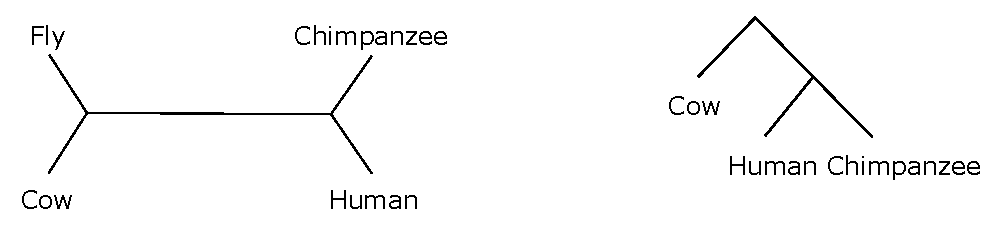
\includegraphics[width=0.9\textwidth]{Figure/outgroup.eps}
\caption{A phylogenetic tree relating four species: human, chimpanzee, gorilla and orangutan. }
\label{fig:outgroup}
\end{figure}

Fig.~\ref{fig:outgroup} shows an example phylogenetic tree among four species: human, chimpanzee, gorilla and orangutan. This evolutionary tree depicts that human and chimpanzee share a common ancestor. As such, we consider humans to be more closely related to chimpanzees than they are to gorillas and orangutans.
%\end{comment}
%\subsubsection{Rooted and unrooted trees} 
In a rooted phylogenetic tree (left part of Fig.~\ref{fig:outgroup}), one vertex $r \in V$ is designated as the root of the tree whereas there is no such designated vertex in an unrooted tree (right part of Fig.~\ref{fig:outgroup}). True evolutionary histories are better represented by a rooted tree. However, identifying the root of an estimated phylogenetic tree is generally a difficult task.

\section{Phylogeny Estimation}

\section{Evaluation of Phylogeny Estimation methods}\label{sec:phyPerf}
The performance of a species tree estimation is evaluated by comparing its output tree to the ground truth (i.e., true species tree provided with the simulated dataset) using False Negative (FN) rate also known as the missing branch rate. FN rate actually expresses (in percentage) the fraction of edges that exist in the latter (i.e., in true tree) but are absent in the former (i.e., in the estimated one). Clearly, the smaller the
value of FN rate, the more desirable it is. Although there are two more common tree error measures (False Positive (FP rate) and Robinson-Foulds (RF) rate), all of them are identical when true and estimated trees are binary. In this thesis, we worked with binary trees only.

\section{Discordance between Gene tree and Species tree}\index{Gene tree discordance}
We now discuss the issue of discordance between a gene tree and species tree and the reasons behind it. A species tree represents the evolutionary history among a set of species via the process of speciation. On the contrary, a gene tree represents the evolution of a particular ``gene" within a group of species. When species are split by speciation, the gene copies within species are also split into separate lineages of descent.  Within each such lineage, the gene trees continue branching and descending through time. Thus, the gene trees are contained within the branches of the species trees~\cite{maddison1997gene}.
However, when gene copies are sampled from various species, the gene tree relating these copies might disagree with the species phylogeny. Fig.~\ref{fig:discordance} shows an example of discordance between a species tree and a gene tree. Here, species $B$ and $C$ are ``sister" species. However, in the gene lineage, $C$ is closer to $D$ than $B$. This discord can arise from the horizontal transfer, incomplete lineage sorting, and gene duplication and extinction~\cite{maddison1997gene}. 

\begin{figure}[!tb]
	\centering
	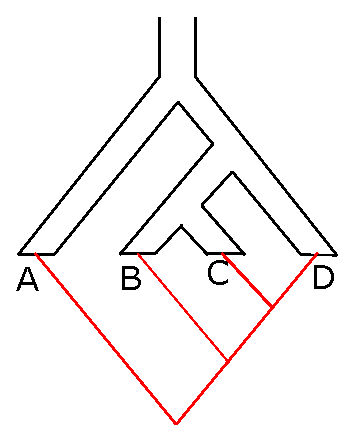
\includegraphics[width=0.33\textwidth]{Figure/discordance.eps}
	\caption{Gene tree-species tree discordance. A species tree (given in block diagram) and a gene tree (given in line diagram) on the same set $\{A,B,C,D\}$ of taxa with different topologies.}
	\label{fig:discordance}
\end{figure}



\subsection{Incomplete Lineage Sorting}\index{Incomplete lineage sorting (ILS)}

%Incomplete lineage sorting (ILS) refers to the failure of two gene lineages to coalesce at their speciation point. Also known as deep coalescence, this process is best understood under the multi-species coalescent (MSC) model~\cite{degnan2006discordance, degnan2005gene}. This model explains the evolutionary process by going backward in time and connecting gene lineages to a common ancestor through a process of ``coalescence" of lineage pairs. This is explained with an example in the Appendix.
%\section{Incomplete Lineage Sorting}%\index{Incomplete lineage sorting (ILS)}

Incomplete lineage sorting (ILS) refers to the failure of two gene lineages to coalesce at their speciation point. Also known as deep coalescence, this process is best understood under the coalescent model~\cite{degnan2006discordance, degnan2005gene}. This model explains evolutionary process by going backwards in time and connecting gene lineages to a common ancestor through a process of ``coalescence" of lineage pairs. In this model, each species is treated as a population of individuals, having a pair of alleles for each gene. The present day variants of a gene (known as alleles) are then traced back in time across successive generations by following the ancestral alleles in the previous generation from which this given alleles evolved. Eventually a point is reached where two alleles coalesce (i.e., they find a common ancestor). The multi-species coalescent (MSC) model is the extension of this general coalescent framework where multiple randomly mating populations corresponding to multiple species are present.
%, nei1987molecular, tajima1983evolutionary, takahata1989gene
\begin{figure}[!tb]
	\centering
	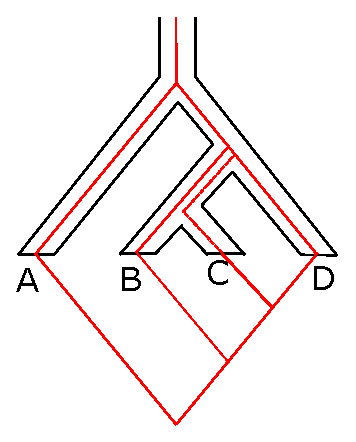
\includegraphics[width=0.33\textwidth]{Figure/ils.eps}
	\caption{Example of gene tree-species tree discordance due to incomplete lineage sorting. Going back in time, the gene copies within species $B$ and $C$ first meet at their corresponding speciation point, but fail to coalesce. Both the lineages (dashed and solid black lines) exist on deeper ancestral branch. The gene from $C$ first coalesces with the gene from species $D$, and subsequently with the gene from $B$.
	}
	\label{fig:ils}
\end{figure}
Under the MSC model, ILS can be a source of gene tree discordance, as the common ancestry of gene copies at a single locus can extend deeper than speciation events. The larger the effective population size and the shorter the branch length of the evolutionary tree, the greater the chance of ILS or deep coalescence to occur~\cite{maddison1997gene}.

Figure~\ref{fig:ils} shows an example of discordance due to ILS. The gene copies within species $B$ and $C$ first meet at their corresponding speciation point as we go back in time. The speciation point is the most recent common ancestor of species $B$ and $C$. However, the gene copies fail to coalesce here. Both of these copies go further back in time, resulting in two gene lineages on deeper ancestral branch. The extra lineage is shown by the dashed red lines in Figure~\ref{fig:ils}. Then the gene from $C$ first coalesces with the gene from species $D$, and subsequently with the gene from $B$.

\begin{comment}
\begin{figure}[!tb]
\centering
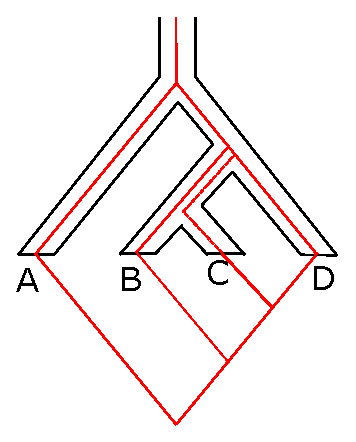
\includegraphics[width=0.33\textwidth]{Figure/ils.eps}
\caption{Example of gene tree-species tree discordance due to incomplete lineage sorting. }
\label{fig:ils}
\end{figure}
Under the MSC model, ILS can be a source of gene tree discordance. Figure~\ref{fig:ils} shows an example of discordance due to ILS. The gene copies within species $B$ and $C$ first meet at their corresponding speciation point as we go back in time. The speciation point is the most recent common ancestor of species $B$ and $C$. However, the gene copies fail to coalesce here. Both of these copies go further back in time, resulting in two gene lineages on a deeper ancestral branch. The extra lineage is shown by the dashed black lines in Figure~\ref{fig:ils}. Then the gene from $C$ first coalesces with the gene from species $D$, and subsequently with the gene from $B$.
\subsubsection{Quartet Score}
The quartet score~\cite{mirarab2014astral} measures the similarity between a candidate species tree $T$ and the input gene trees, and is computed as follows. Each input gene tree is decomposed into its induced set of quartet trees (i.e., unrooted trees formed by picking four leaves). The quartet support score of a given candidate species tree $T$ is the total, overall the input gene trees, of the number of induced quartet trees that $T$ agrees with. This score is maximized by ASTRAL to estimate the species tree. 

\subsubsection{Triplet Score}
The triplet score~\cite{islam2019stelar}, similar to quartet score, counts the number of induced triplet trees (i.e., rooted trees formed by picking three leaves) of the candidate species tree that agrees with the input gene trees. This criterion is maximized by STELAR. 

\subsubsection{Pseudo-likelihood}
It measures the likelihood of a candidate species tree given the triplet distribution of the input gene trees and maximized by MP-EST~\cite{mpest} as an estimator of the species tree.
\end{comment}

\subsection{Statistical consistency}\index{Statistical consistency}

A species tree reconstruction method is said to be statistically consistent under a particular model of evolution if the probability of returning the true species tree converges to one as the amount of data increases. Let the set of genes in a study be $\mathcal{G} = \{g_1, g_2, \dots, g_M\}$. Let $s_i$ be the number of sites in $g_i$ ($1 \leq i \leq M$). Then A species tree estimation method is statistically consistent if the estimated species tree converges to the true species tree as $M \rightarrow \infty$, $\underset{1 \leq i \leq M}{s_i} \rightarrow \infty$.


\subsection{Optimization criteria for species tree estimation}
Various criteria are statistically consistent estimators of the true species tree under the MSC model. Each of them measures how well a candidate species tree can summarize the input gene trees. Three examples are as follows:
\begin{itemize}
	\item Quartet score (maximized by ASTRAL~\cite{mirarab2014astral}): The quartet score of a given candidate species tree $T$ is the total, across all the input gene trees, of the number of induced quartet trees that $T$ agrees with. This score is maximized by ASTRAL to estimate the species tree.
	\item Triplet score (maximized by STELAR~\cite{islam2019stelar}): Similar to quartet score, it counts the number of induced triplet trees (i.e., rooted trees formed by picking three leaves) of the candidate species tree that agrees with the input gene trees.
	\item Pseudo-likelihood (maximized by MP-EST~\cite{mpest}): It measures the likelihood of a candidate species tree given the triplet distribution of the input gene trees.
\end{itemize}


\section{Multiple Sequence Alignment}
Multiple sequence alignment (MSA) task seeks to arrange three or more nucleotide/protein sequences to infer homology, considering various biological phenomena (i.e., evolutionary history, 3D structure etc.). The output is a matrix in which the input nucleotide/protein sequences are the rows and each column (i.e., site) has characters which are homologous which means all those letters descend from the same letter of a common ancestor). The aligned sequences reflect historical substitution, insertion and deletion of genetic materials which are represented as gaps. Accurately recovering these properties through MSA is necessary to accomplish a biological objective such as inferring the evolutionary history relating the sequences known as phylogenetic trees. While computing MSAs, various computational methods and criteria are used to make hypotheses about homology. But the goal of MSA is entirely biological. Figure~\ref{fig:msa_io} illustrates this problem using an example where four hypothetical protein sequences are to be aligned by placing ``necessary'' gaps. %In this work, we focus on the MSA tasks in the context of phylogeny estimation which usually functions in two steps. Firstly, the given sequences are aligned using an MSA tool, thereafter a phylogenetic tree is inferred on obtained alignment. The goodness of estimated phylogenetic trees largely rely on the properties of the corresponding alignment. Thus, choosing the ``most appropriate'' MSA method  is important in the phylogenetic context.

\begin{figure}[!htbp]
	\centering
	\includegraphics[width=0.8\textwidth]{cybernatics/Figure/msa_io}
	\caption{A hypothetical instance of MSA task with four protein sequences.} 
	\label{fig:msa_io}
\end{figure}

\graphicspath{{cybernatics/supp/}}

% Table generated by Excel2LaTeX from sheet 'acronym'
\begin{table}[htbp]
	\centering
	%\begin{adjustwidth}{-0.2cm}{}
	\scriptsize
	\caption{Alphabetic list of acronyms used in this study.}
	\begin{tabular}{|L{2cm}|L{13cm}|}
		\hline
		\multicolumn{1}{|c|}{Acronym} & \multicolumn{1}{c|}{Usage} \\
		\hline
		23S.E & A biological rRNA dataset  \\
		\hline
		23S.E.aa\_ag & A biological rRNA dataset  \\
		\hline
		BBXY0MN & MN$^{th}$ BAliBASE instance under RVXY group \\
		\hline
		Clustal $\Omega$ & A state-of-the-art MSA method \\
		\hline
		Clustal W & A state-of-the-art MSA method \\
		\hline
		FN rate & False negative rate, measures quality of a phylogenetic tree w.r.t. the reference tree \\
		\hline
		FSA   & A state-of-the-art MSA method \\
		\hline
		Gap   & No. of gaps, an objective function that measures goodness of an MSA \\
		\hline
		GapCon & Concentration of gaps, an objective function that measures goodness of an MSA \\
		\hline
		Kalign & A state-of-the-art MSA method \\
		\hline
		MAFFT & A state-of-the-art MSA method \\
		\hline
		ML & Maximum likelihood approach for inferring a phylogenetic tree from an MSA\\
		\hline
		MSA   & Multiple sequence alignment \\
		\hline
		MUSCLE & A state-of-the-art MSA method \\
		\hline
		NSGA-II & A multi-objective metaheuristics  \\
		\hline
		NSGA-III & A multi-objective metaheuristics which an improved version of NSGA-II to handle more than three objective functions  \\
		\hline
		PASTA & A state-of-the-art MSA method \\
		\hline
		PRANK & A state-of-the-art MSA method \\
		\hline
		ProbCons & A state-of-the-art MSA method \\
		\hline
		R0   & A random replicate of 100-taxon simulated dataset \\
		\hline
		R14   & A random replicate of 100-taxon simulated dataset \\
		\hline
		R19   & A random replicate of 100-taxon simulated dataset \\
		\hline
		R4   & A random replicate of 100-taxon simulated dataset \\
		\hline
		R9   & A random replicate of 100-taxon simulated dataset \\
		\hline
		RetAlign & A state-of-the-art MSA method \\
		\hline
		RV11  & One of the six groups of BAliBASE 3.0 benchmark \\
		\hline
		RV12  & One of the six groups of BAliBASE 3.0 benchmark \\
		\hline
		RV20  & One of the six groups of BAliBASE 3.0 benchmark \\
		\hline
		RV30  & One of the six groups of BAliBASE 3.0 benchmark \\
		\hline
		RV40  & One of the six groups of BAliBASE 3.0 benchmark \\
		\hline
		RV50  & One of the six groups of BAliBASE 3.0 benchmark \\
		\hline
		SimG  & Similarity based on gap columns, an objective function that measures goodness of an MSA \\
		\hline
		SimNG & similarity based on non-gap columns, an objective function that measures goodness of an MSA \\
		\hline
		SOP   & Sum of pairs, an objective function that measures goodness of an MSA without using the reference alignment\\
		\hline
		SP score & Sum-of-pair score, measures quality of an MSA w.r.t. the reference alignment  \\
		\hline
		T-Coffee & A state-of-the-art MSA methods \\
		\hline
		TC & No. of totally aligned columns, an objective function that measures goodness of an MSA without using the reference alignment \\
		\hline
		TC score & Total-column score, measures quality of an MSA w.r.t. the reference alignment  \\
		\hline
		wSOP  & Weighted sum of pairs, an objective function that measures goodness of an MSA \\
		\hline
	\end{tabular}%
	\label{tab:acronyms}%
	%\end{adjustwidth}
\end{table}%

\section{Objective functions for MSA}
\label{sec:objective _function}
There are numerous objective functions defined for MSA in the literature. We identify the following widely used objective functions from the recent works and briefly discuss their feasibility in MSA:

\begin{itemize}
	
	\item \textbf{Maximize sum of pairs score}~\cite{seeluangsawat2005multiple, da2010alineaga}:  
	This is an extension of pairwise sequence alignment score. Pairwise score is calculated for each pair of aligned sequences. Then, we calculate the total score by summing pairwise scores of all possible pairs. In Figure \ref{fig:pairwise}, the pairwise score is calculated by considering the elements of the same columns of two aligned sequences with the scoring or substitution matrix $\delta$. There are some standard substitution matrices for biological sequences at~\url{ftp://ftp.ncbi.nih.gov/blast/matrices/}.
	
	
	\begin{figure}[!htbp]
		\begin{adjustwidth}{-0.2cm}{}
			\centering
			\begin{subfigure}[b]{0.5\columnwidth}
				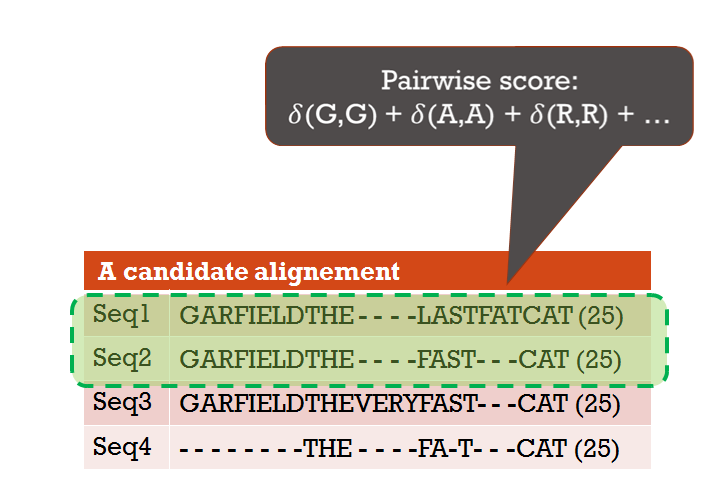
\includegraphics[width=\columnwidth]{Figure/pairwise}
				\caption{Pairwise score of two aligned sequences.}
				\label{fig:pairwise}
			\end{subfigure}	
			\begin{subfigure}[b]{0.5\columnwidth}
				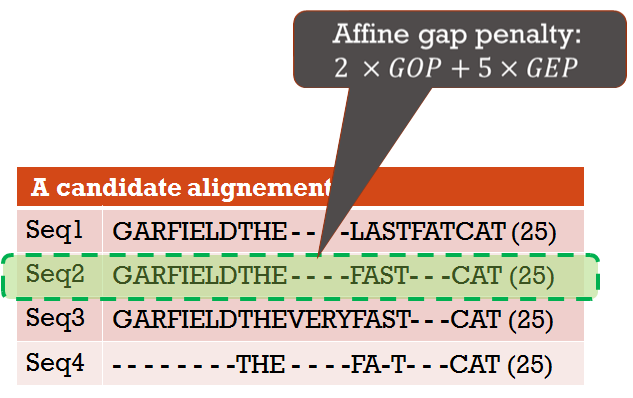
\includegraphics[width=\columnwidth]{Figure/agp}
				\caption{Affine gap penalty of an aligned sequence.}
				\label{fig:agp}
			\end{subfigure}
			\begin{subfigure}[b]{0.5\columnwidth}
				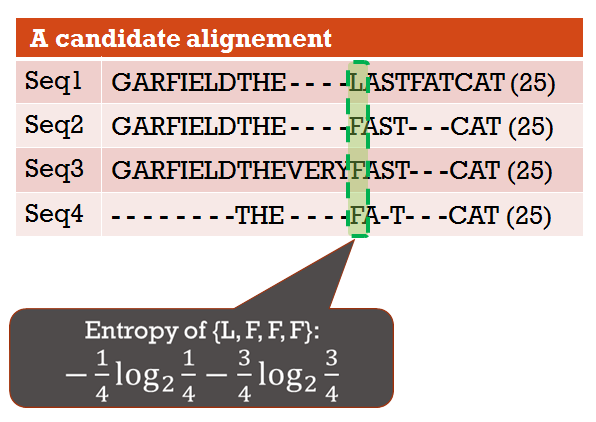
\includegraphics[width=\columnwidth]{Figure/entropy_score}
				\caption{Entropy of a column of alignment.}
				\label{fig:entropy}
			\end{subfigure}
		\end{adjustwidth}
		\caption{Three objective functions for MSA. The example alignment is adopted from~\citep{rubio2016hybrid}.}
		\label{fig:msa_obj}
	\end{figure}
	
	\item \textbf{Minimize entropy}~\cite{soto2014multi}: 
	Entropy is a measurement of dissimilarity in the same columns of different aligned sequences. When all the columns contain same element, the entropy is minimum \(0\). Again, the entropy is maximum \(1\) when every element is different. Total entropy is calculated by summing up entropy values of all columns. Figure \ref{fig:entropy} demonstrates the calculation of entropy for a single column. The problem with this function is that, while calculating entropy researchers treat gap as a separate character without proper justification.
	
	\item \textbf{Minimize affine gap penalty}~\cite{seeluangsawat2005multiple, kaya2014multiple, zhu2016novel, rani2016multiple}: 
	Affine gap penalty assigns different penalty for opening a gap ($GapOpeningPenalty, GOP$) and extending a gap ($GapExtension\-Penaly, GEP$) while computing gap penalty for a particular sequence. Then finally, summation of gap penalties of all sequences is to be minimized. An example is demonstrated in Figure \ref{fig:agp} showing the calculation of gap penalty of one sequence. Here two ideas (i.e. percentage of gap and concentration of gap) are combined without explanation. Also researchers face trouble to fix the value of two penalties.
	
	\item \textbf{Maximize weighted sum of pairs score with affine gap penalties}~\cite{rubio2016hybrid, rubio2016bee}:  
	Here two objectives are combined in the form: weighted sum of pairs score - affine gap penalty. To calculate weighted sum of pairs score, score of each pair of characters are multiplied by the sequence weight between that the corresponding two sequences. This weight is computed using the Levenshtein distance between two non-aligned sequences. Levenshtein distance is the is the minimum number of insertions, deletions or substitutions needed to convert one sequence into the other. 
	
	\item \textbf{Maximize number of totally aligned columns}~\cite{ortuno2013optimizing, da2010alineaga, rubio2016hybrid, rubio2016bee, ortuno2013optimizing, zambrano2017comparing}:
	Maximizing the number of totally aligned columns is the most simple used objective. But for input data comprising large number of taxa, its value is confined to a few values.
	
	\item \textbf{Minimize percentage of gaps}~\cite{abbasi2015local, ortuno2013optimizing, zambrano2017comparing}:
	High percentage of gaps means the sequences had to be significantly modified to align with each other. This is used as a minimizing objective function to find a better candidate solution. It can be also considered as percentage of non-gaps.
	
	\item \textbf{Maximize similarity}~\cite{kaya2014multiple, rani2016multiple}:
	%Similarity performs a measure of structural similarity among all sequences defining an individual. 
	For each column of MSA, similarity considers the ratio of the dominant character. This ratio is averaged over all columns. The closer the value of similarity is to one, the larger the probability that the candidate alignment will be discovered as the best possible alignment. Here we find similar problem as with entropy. Researchers discard gap while calculating ratio of characters in a column without sound reasoning. 
	
\end{itemize}

%\section{Multi-objective optimization}
\section{Multi-objective metaheuristics}
\label{sec:mop}
While optimizing multiple objective functions simultaneously, a multi-objective metaheuristics determines a set of solutions (instead of a single solution) which represents the best-possible compromise of all objectives. A solution is said to dominate another one if and only if it is equal to that solution in all objectives and also better than that in at least one objective. A solution is said to be Pareto optimal if no other solutions can dominate it. The set of all Pareto optimal solutions is called Pareto set and the image of pareto set in the objective space is known as Pareto front. However, practically a multi-objective metaheuristics aims to approximate the Pareto front as precisely as possible with a finite number of solutions.

%\subsection{Evolutionary algorithms}
Among metaheuristics, multi-objective evolutionary algorithms (MOEAs) are well-suited to solve multi-objective optimization problems~\cite{yang2013grid}. MOEAs deal with a set of possible solutions (known as population) at once which allows finding several members of the Pareto front in a single run of the algorithm. Moreover, they are  black-box optimization methods which do not need particular assumptions like continuity or differentiability of the decision space. 

%So the goal of a multi-objective metaheuristics is to output a set of solutions instead of a single solution., evolutionary algorithms (EAs) are population-based, They are well suited for multi-objective optimization. 

\begin{algorithm}[!htb]
	\caption{A General structure of MOEA}
	\begin{algorithmic}[1]\label{alg:MaOEA}
		\STATE{Randomly generate the initial population $ P_0 $}
		\STATE{Evaluate the objective functions of each individual in $ P_0 $}
		\STATE{$t \leftarrow 0$}
		\WHILE{$t <$ maximum value of $t$} 
		\STATE{Generate offspring population $ Q_t $ by applying \textit{Crossover} and \textit{Mutation} on $ P_t $}
		\STATE{Evaluate the objective functions of each individual in $ Q_t $}
		\STATE{Produce generation $ P_{t+1} $ from $ P_t $ and $ Q_t $ using \textit{Ranking scheme}}
		\STATE{$t \leftarrow t + 1$ }
		\ENDWHILE
	\end{algorithmic}
\end{algorithm}

A general structure of MOEAs is summarized in Algorithm \ref{alg:MaOEA}. Here the \textit{Crossover} and \textit{Mutation} are popularly known as genetic operators. They generate offspring (new solutions) from parents (existing solutions). These are problem-specific and designed based on the actual problem to be solved. \textit{Ranking scheme} is used to choose appropriate solutions to form the next generation. This is problem-independent concept and provided by the developers of a specific algorithm. In this study, we considered the three widely used MOEAs for multi-objective optimization. We briefly describe them as follows.

\begin{enumerate}[label=(\alph*)]
	
	\item NSGA-II~\citep{deb2002fast} follows the classical structure of a generational genetic algorithm. At first, it applies the typical genetic operators (selection, crossover, and mutation) on the current population to fill an auxiliary population. Then it builds the next-generation by incorporating the best individuals from both the current and auxiliary populations according to a Pareto ranking and the crowding distance operator. Perhaps it is the most commonly used algorithm for solving optimization problems having two or three objective functions. 
	
	\item NSGA-III~\citep{deb2014evolutionary} is designed to handle a large number of objective functions. The skeleton of NSGA-III remains similar to its predecessor NSGA-II with notable changes in its selection mechanism. At each generation, it produces an offspring population from the current population by applying genetic operators. These two populations are merged to form a new population using the selection mechanism. NSGA-III continues to use Pareto dominance as the primary selection criterion to promote convergence. But it substitutes the crowding distance operator in NSGA-II with a clustering operator aided by a set of well-distributed reference points as the secondary selection criterion to maintain diversity. NSGA-III has been shown to perform reasonably.
	%NSGAIII has been shown to perform reasonably on handling a large number of objective functions~\cite{deb2014evolutionary}.
	
	\item MOEA/D~\citep{zhang2007moea} is a representative decomposition based MOEA. Unlike Pareto dominance based methods (e.g., NSGA-II, NSGA-III), It decomposes the original problem into many single-objective subproblems using an aggregation function and a series of weight vectors defining the relative importance of different objectives. %We use the Das and Dennis's procedure~\cite{das1998normal} for generating uniform weight vectors, which are evenly distributed along the 7-dimensional unit hyper-plane. 
	Then it deals with these subproblems in a collaborative manner. Neighborhood relations among these subproblems are defined based on the similarity between their weight vectors. 
	%When optimizing a subproblem, the local information from its neighboring subproblems is shared. 
	Each subproblem maintains an individual which could be the best individual found so far for it. The algorithm generates a new individual for each subproblem by performing genetic operators on some of its neighboring individuals. The current individual of both the considered subproblem and its neighbors will be updated if the new individual is better than their current one. %The procedure of MOEA/D for TNDP is presented in Algorithm~\ref{alg:moead}.	(i.e., the individuals of its neighboring subproblems) that combines all objectives
	For MSA, we adopt the MOEA/D configuration used by~\citep{zhu2015novel}.  
\end{enumerate} 



%\subsection{Our multi-objective metaheuristic framework}
%\label{sec:mof}
% Table generated by Excel2LaTeX from sheet 'multi-pc'

\begin{comment}
\subsubsection{Solution Initialization}
Instead of initializing solutions randomly, which is the usual practice in metaheuristics, we seed the initial population with alignments generated by nine state-of-the-art MSA tools. These tools are listed in Table~\ref{tab:msa_tools}. We create the required number of initial solutions by randomly mixing and modifying those nine alignments. 
%Among these tools PASTA is the most recently developed. Due to its simultaneous estimation of alignment and phylogenetic tree, it is expected to be the most robust.

\begin{table*}[htbp]
\small
\centering
\caption{List of state-of-the-art MSA tools that we used initialize the metaheuristics.}
\begin{tabular}{|l|l||l|l|}
\hline
\multicolumn{2}{|c||}{For nucleotide sequences} & \multicolumn{2}{c|}{For protein sequences} \\
\hline
\multicolumn{1}{|c|}{Tool} & \multicolumn{1}{c||}{Version} & \multicolumn{1}{c|}{Tool} & \multicolumn{1}{c|}{Version} \\
\hline
FSA~\citep{bradley2009fast} & 1.15.9 & FSA   & 1.15.9 \\
\hline
PASTA~\citep{mirarab2015pasta} & 1.7.8 & PASTA & 1.7.8 \\
\hline
T-Coffee~\citep{notredame2000t} & 11.00 & T-Coffee & 11.00 \\
\hline
MAFFT~\citep{katoh2002mafft} & 7.31  & MAFFT & 7.245 \\
\hline
Clustal W~\citep{thompson1994clustal} & 2.1   & Clustal W & 2.1 \\
\hline
Clustal $ \Omega $~\citep{sievers2011fast} & 1.2.4 & RetAlign~\citep{szabo2010reticular} & 1.0 \\
\hline
MUSCLE~\citep{edgar2004muscle} & 3.8.31 & MUSCLE & 3.8.31 \\
\hline
PRANK~\citep{loytynoja2005algorithm} & 0.170427 & ProbCons~\citep{do2005probcons} & 1.12 \\
\hline
Kalign~\citep{lassmann2008kalign2} & 2.03  & Kalign & 2.04 \\
\hline
\end{tabular}%
\label{tab:msa_tools}%
\end{table*}%

\subsubsection{Genetic Operator}
Both of our metaheuristics used the same genetic operator (i.e. mutation and crossover), which were used by~\citealp{ortuno2013optimizing}. \citealp{zambrano2017multi} illustrated their functions. Here we provide a short description of these operators. 

The mutation operator is termed as closed gap shifting, where consecutive gaps are randomly chosen and shifted to another random position in a sequence. This shifting may result columns having only gaps which are then removed. Thus this mutation tries to reduce the number of gaps in the MSA.

The crossover operator is the single-point crossover over alignments proposed by~\citealp{da2010alineaga}. The operator randomly selects a column from one parent to split it into two blocks (let us refer to them P1a and P1b). The same selected positions are located in the other parent (which are not necessarily in the same column) and is tailored so that the right piece can be joined to the left piece of the first parent and vice versa (P2a and P2b). Finally, the selected blocks are exchanged between these two parents to create two new individuals with the combination of the blocks: [P1a + P2b] and [P1a + P1b]. After that, any empty space that appears at the junction point is filled with gaps.
%\subsubsection{Multi-objective evolutionary algorithm}
%\subsubsection{Parameter Configuration}
\end{comment}

\begin{comment}


\section{Evaluation of estimated alignments}
\label{sec:msa_eval}
We evaluate estimated alignments with respect to reference alignment using two well-known alignment quality scores called TC score and SP score. These two scores are defined below:
\begin{itemize}
	\item TC score is the ratio of the number of correctly aligned columns in the estimated alignment to the total number of aligned columns in the reference alignment. This is also known as column score.
	
	\item SP score is the ratio of the number of aligned pairs in the estimated alignment to the total number of aligned pairs in the reference alignment.
	
	%\item Pairs score is the mean of SP-score and Modeler. SP-Score is the ratio of the number of aligned pairs to the total number of aligned pairs in the reference alignment. And Modeler is very similar to the SP-score where we take the ratio of the number of aligned pairs to the total number of aligned pairs in the estimated alignment  	
\end{itemize}
For both the measures, higher value implies better score.

\section{Phylogenetic tree estimation}
\label{sec:tree_estimation}
For each of the generated alignment we estimate the phylogenetic tree using Maximum Likelihood (ML) method which is the standard way of estimating phylogenetic tree from sequence data~\cite{liu2011raxml}. FastTree\citep{price2010fasttree} and RAxML~\citep{stamatakis2014raxml} are the most widely used software for this purpose. FastTree can produce output very quickly with little (and in some cases no) degradation in tree accuracy, as compared to RAxML~\cite{liu2011raxml}. In this study we had to estimate a large number of phylogenetic trees. So we choose FastTree over RAxML.
%We used a popular tool named FastTree-2 developed by \citep{price2010fasttree}. %It is publicly available at \url{http://www.microbesonline.org/fasttree/}.

\section{Evaluation of phylogenetic tree}
\label{sec:tree_eval}
We evaluate the quality of each estimated ML tree with respect to the true phylogenetic tree using a widely used measure known as the False Negative (FN) rate. FN rate is the percentage of edges present in the true tree but missing in the estimated tree. So a small value of FN rate is desirable. Although there are two more common tree error measures (False Positive (FP rate) and and Robinson-Foulds (RF) rate), all of them are identical when true and estimated trees are binary~\citep{warnow2017computational}. In this study we worked with binary trees only. %as a quality measure, 

\section{Evaluation of objective functions}
\label{sec:obj_eval}
In the context of phylogeny estimation, a desired objective function for MSA should lead to such alignments which can produce highly accurate (having small FN rate) ML trees. Considering this fact, we try to evaluate the effectiveness of an objective function by studying how its values are associated with the corresponding FN rates. The objective function that frequently exhibits positive correlation with FN rate is predicted to be a good optimization criteria. To accomplish this, we fit multiple linear regression model to calculate the degree of association (i.e., regression coefficient) between an objective and FN rate. Then we apply t-test, with null hypothesis that there is no association, to check the significance of individual regression coefficients. It should be noted that, such regression results does not necessarily indicate the strength of an objective as an optimization criterion. However, such results can definitely be utilized as the starting point for experimentation for further validation.

\end{comment} 



\graphicspath{{cybernatics/}}

\chapter{Multi-objective Formulation of MSA for Phylogeny Inference} \label{ch:cybernatics}
 Multiple sequence alignment (MSA) is a preliminary task for estimating phylogenies. It is used for homology inference among the sequences of a set of species. Generally, MSA task is handled as a single-objective optimization process.
The alignments computed under one criterion may be different from the alignments generated by other criteria, inferring discordant homologies and thus leading to different hypothesized evolutionary histories relating the sequences. The multi-objective (MO) formulation of MSA has recently been advocated by several researchers, to address this issue. An MO approach independently optimizes multiple (often conflicting) objective functions at the same time and outputs a set of competitive alignments. However, no conceptual or experimental rational from a real-world application perspective has been reported so far for any MO formulation of MSA. This chapter work investigates the impact of MO formulation in the context of an important scientific problem, namely, phylogeny estimation. Employing popular evolutionary MO algorithms, we show that (a) trees inferred based on alignments produced by the existing MSA methods used in practice are substantially worse in quality than the trees inferred based on the alignments output by an MO algorithm and (b) even high quality alignments (according to popular measures available in the literature) may fail to achieve acceptable accuracy in generating phylogenetic trees.      
Thus, we essentially ask the following natural question: ``Can a phylogeny-aware (i.e., application-aware) metric guide in selecting appropriate MO formulations to ensure better phylogeny estimation?" Here we report a carefully designed extensive experimental study that positively answers this question. 


\section{Introduction}
\label{sec:introducntion}
%Multiple sequence alignment (MSA) task seeks to arrange three or more nucleotide/protein sequences to infer homology, considering various biological phenomena (i.e., evolutionary history, 3D structure etc.). The output is a matrix in which the input nucleotide/protein sequences are the rows and each column (i.e., site) has characters which are homologous which means all those letters descend from the same letter of a common ancestor). The aligned sequences reflect historical substitution, insertion and deletion of genetic materials which are represented as gaps. Accurately recovering these properties through MSA is necessary to accomplish a biological objective such as inferring the evolutionary history relating the sequences known as phylogenetic trees. While computing MSAs, various computational methods and criteria are used to make hypotheses about homology. But the goal of MSA is entirely biological. Figure~\ref{fig:msa_io} illustrates this problem using an example where four hypothetical protein sequences are to be aligned by placing ``necessary'' gaps. 
%
%
%\begin{figure}[!htbp]
%	\centering
%\includegraphics[width=0.6\textwidth]{Figure/msa_io}
%\caption{A hypothetical instance of MSA task.} 
%		\label{fig:msa_io}
%\end{figure}
In this thesis, we focus on the MSA tasks in the context of phylogeny estimation which usually functions in two steps. Firstly, the given sequences are aligned using an MSA tool, thereafter a phylogenetic tree is inferred on obtained alignment. The goodness of estimated phylogenetic trees largely rely on the properties of the corresponding alignment. Thus, choosing the ``most appropriate'' MSA method  is important in the phylogenetic context.

\subsection{Can an application-aware measure guide towards better
phylogeny estimation?}
Previously several researchers (\citep{redelings2005joint, ashkenazy2018multiple}) attempted to improve the phylogeny estimation focusing on MSA computation. While they also agree with our core idea that the nature of MSA computation may influence the outputs (in a domain specific manner) and thereby provided proof of concept. We differ from them by adopting the multi-objective (MO) optimization.
We are motivated from the fact that the alignment generated by optimizing one objective function may be different from the alignments estimated under other objectives. Consequently, this may infer discordant homologies thereby leading to different and often conflicting evolutionary histories relating to the species under consideration. This issue can be addressed by an MO approach that generates a set of alternative alignments by simultaneously optimizing multiple (often conflicting) objectives. But, we are confronted with the challenge of choosing suitable measures/metries to optimize from among a variety of objective functions in literature.
So, we ask the obvious question whether the generic metrics, widely used for assessing the alignment quality, will accurately represent the level of acceptance in the context of a specific application domain, i.e., in our case, phylogeny estimation.
This question has indeed received some discussions, albeit shallow and incomplete, in several studies (\citep{mirarab2015pasta, liu2009rapid}). However, we are not aware of any systematic investigation in the literature to this end. 



This paper, systematically and with scientific rigour, investigates whether a domain-specific performance measure (unlike general-purpose alignment quality measures) can direct us better to find proper MO formulations or tools for MSA when the goal is to infer phylogeny. We suggest a multivariate linear regression based methodology to assess the potential utility of a MO formulation of MSA. Then, following our methodology, we obtained two bi-objective formulations that are capable of yielding better phylogenetic trees than several existing MSA tools.
We perform extensive experimentation with simulated as well as biological datasets and analyze their performance based on quality measures of alignment as well as phylogenetic tree. 
To the best of our knowledge, this is the first work on devising an application-aware MO formulation for tackling MSA. We presented some preliminary results in~\cite{nayeem2019phylogeny}.



\section{Related Works}
\label{sec:literature}
Here we present a concise review of the preceding works relevant to the theme of this chapter. We concentrate on existing MSA methods along with multi-objective (MO) metaheuristics. For a more comprehensive review, readers can be referred to~\citep{warnow2017computational}.

There exists many methods/tools for computing MSAs in the literature. These methods can be loosely classified into three groups, namely, progressive, consistency-based and iterative methods. Also, many tools combine more than one methods. Progressive method computes the alignment in a ``bottom-up'' fashion by aligning pairs of sequences with the help of a guide tree. It is the basis of numerous MSA methods, including, but not limited to, RetAlign~\citep{szabo2010reticular}, Clustal $\Omega$~\citep{sievers2011fast}, PRANK~\citep{loytynoja2005algorithm}, FSA~\citep{bradley2009fast},  Kalign~\citep{lassmann2008kalign2}, etc. 



A consistency-based method builds a collection of pairwise alignments to aid the generation of an overall accurate alignment. T-Coffee~\citep{notredame2000t}, ProbCons~\citep{do2005probcons}, ProbAlign~\citep{roshan2006probalign} etc. are the representatives of this category. And to attain reliable alignments, the iterative methods attempt to correct the impact of mistakes done at the initial phases by repeating certain critical steps. MAFFT~\citep{katoh2002mafft}, MUSCLE~\citep{edgar2004muscle}, MUMMALS~\citep{pei2006mummals}, ProbCons etc. are some examples of such techniques. Also, we find some ``meta-methods'' in this category, such as, SAT\'e~\citep{liu2009rapid} and PASTA~\citep{mirarab2015pasta}. A tool belonging to this category  co-estimates alignments and phylogenetic trees exploiting existing tools. These are quite popular and widely used in practice. To achieve scalability, they employ a divide-and-conquer approach. The widely accepted way of evaluating the operation of an MSA method is to compare and evaluate the output alignment produced thereby against the reference alignment. Probably the most popular measures used for this purpose are the so called sum-of-pair score (i.e., SP score) and total-column score (i.e., TC score)~\citep{warnow2017computational}. They will be defined shortly in a subsequent section.


The MSA datasets of the current post-genomic era have raised several unprecedented challenges to the scientists. Generally, a default parameter setting is suggested for each MSA method to align any data with reasonable correctness. However, the default configuration cannot assure the best performance across all types of datasets~\citep{rubio2018characteristic}. As an example, a parameter in ProbCons may be cited which controls how many times the refinement passes are done iteratively: while the default value is set to 100, this can vary between zero to 1000. By tuning parameters, better results may be achieved for a particular dataset. Nevertheless, a method cannot beat others across different instances despite having its best parameter setting. 

So we observe the appearance of new methods that combine the strength of different existing tools~\citep{thompson2011comprehensive}. Metaheuristics are one of such methods which can exploit the outputs of different methods to generate superior solutions. The success of such a metaheuristic technique relies on the choice of appropriate optimization objective that is able to help selecting better solutions from among the alternatives and thereby guide the search process towards optimal solutions of MSA. And it is sensible to consider multiple objectives at once as any single one solely cannot effectively address the challenges posed by various datasets. We find that MO techniques are being used effectively to address various real-wold problems in several different domains~\cite{8955943, 9098079, 8984353, 8842602}.
Thus tackling MSA with MO approach is worth investigating.


Recently we notice several works (\citep{da2010alineaga, ortuno2013optimizing, soto2014multi, abbasi2015local, rubio2016hybrid,zambrano2017comparing, rubio2018characteristic}) on the MO formulation for MSA – suggesting upto four objectives to identify and measure the various features of alignment. Maximizing the sum of pairs score may be regarded as the most well-known objective function.
Perhaps the most well-known objective function is the maximization of the sum of pairs score. It evaluates every pair of aligned sequences with the help of a substitution matrix that is expected to represent the dataset traits. Another common  objective to maximize is the totally conserved columns which counts the columns having the same character across all rows. But we know that such columns do not necessarily indicate homology.
Besides, several studies consider minimizing the number of gaps to keep the resultant alignment compact. Also various forms of gap penalties are minimized that adopts a penalization scheme based on gap pattern. Furthermore, entropy and similarity are two minimization objectives which evaluate each column of an alignment. They try to quantify how homogeneous are the letters contain in the same column. It should be noted that, the reference alignment is not allowed to use in the calculation of any objective function. 

We find some unresolved issues in existing studies that advocated the MO formulation of MSA. Firstly, insufficient conceptual or experimental justification for selecting a specific objective to optimize. Next, lack of concrete reasoning for the employment of the two widely accepted performance measures: SP score and TC score. It seems rather reasonable on the contrary that the measures to evaluate the performance should have  reflected the true intent of the MSA task: 
if the purpose is phylogeny inference, then, the success should be evaluated based on a measure that can reliably express the `goodness' and `utility' of the constructed phylogenetic tree. Finally, the dataset used in experimentation, particularly the number of species used therein, is relatively small (i.e., below 50 species).


In this chapter, our context is phylogeny estimation and we aim to address the above mentioned limitations of MO optimization for MSA in that context. In particular, we propose a new method that leverages multivariate linear regression for selecting application-aware MO formulations. We notice several prior efforts (e.g.,~\citep{lu2012classification, zhou2005study}) on regression-assisted optimization approaches. However, unlike ours, those works focused on constructing a surrogate model, by applying regression techniques, for computationally expensive fitness evaluation.


  \section{Methods}
\label{sec:methods}
Because we deal with numerous objective functions, exisitng MSA methods and datasets, a reader is exposed to an over-preponderance of acronyms and short-cut notations. Therefore, for the sake of ease in exposition and understanding, Table~\ref{tab:acronyms} of the supplementary file alphabetically lists all the acronyms used in this paper along with their intended usage.

\begin{figure}[!htbp]
	\centering

	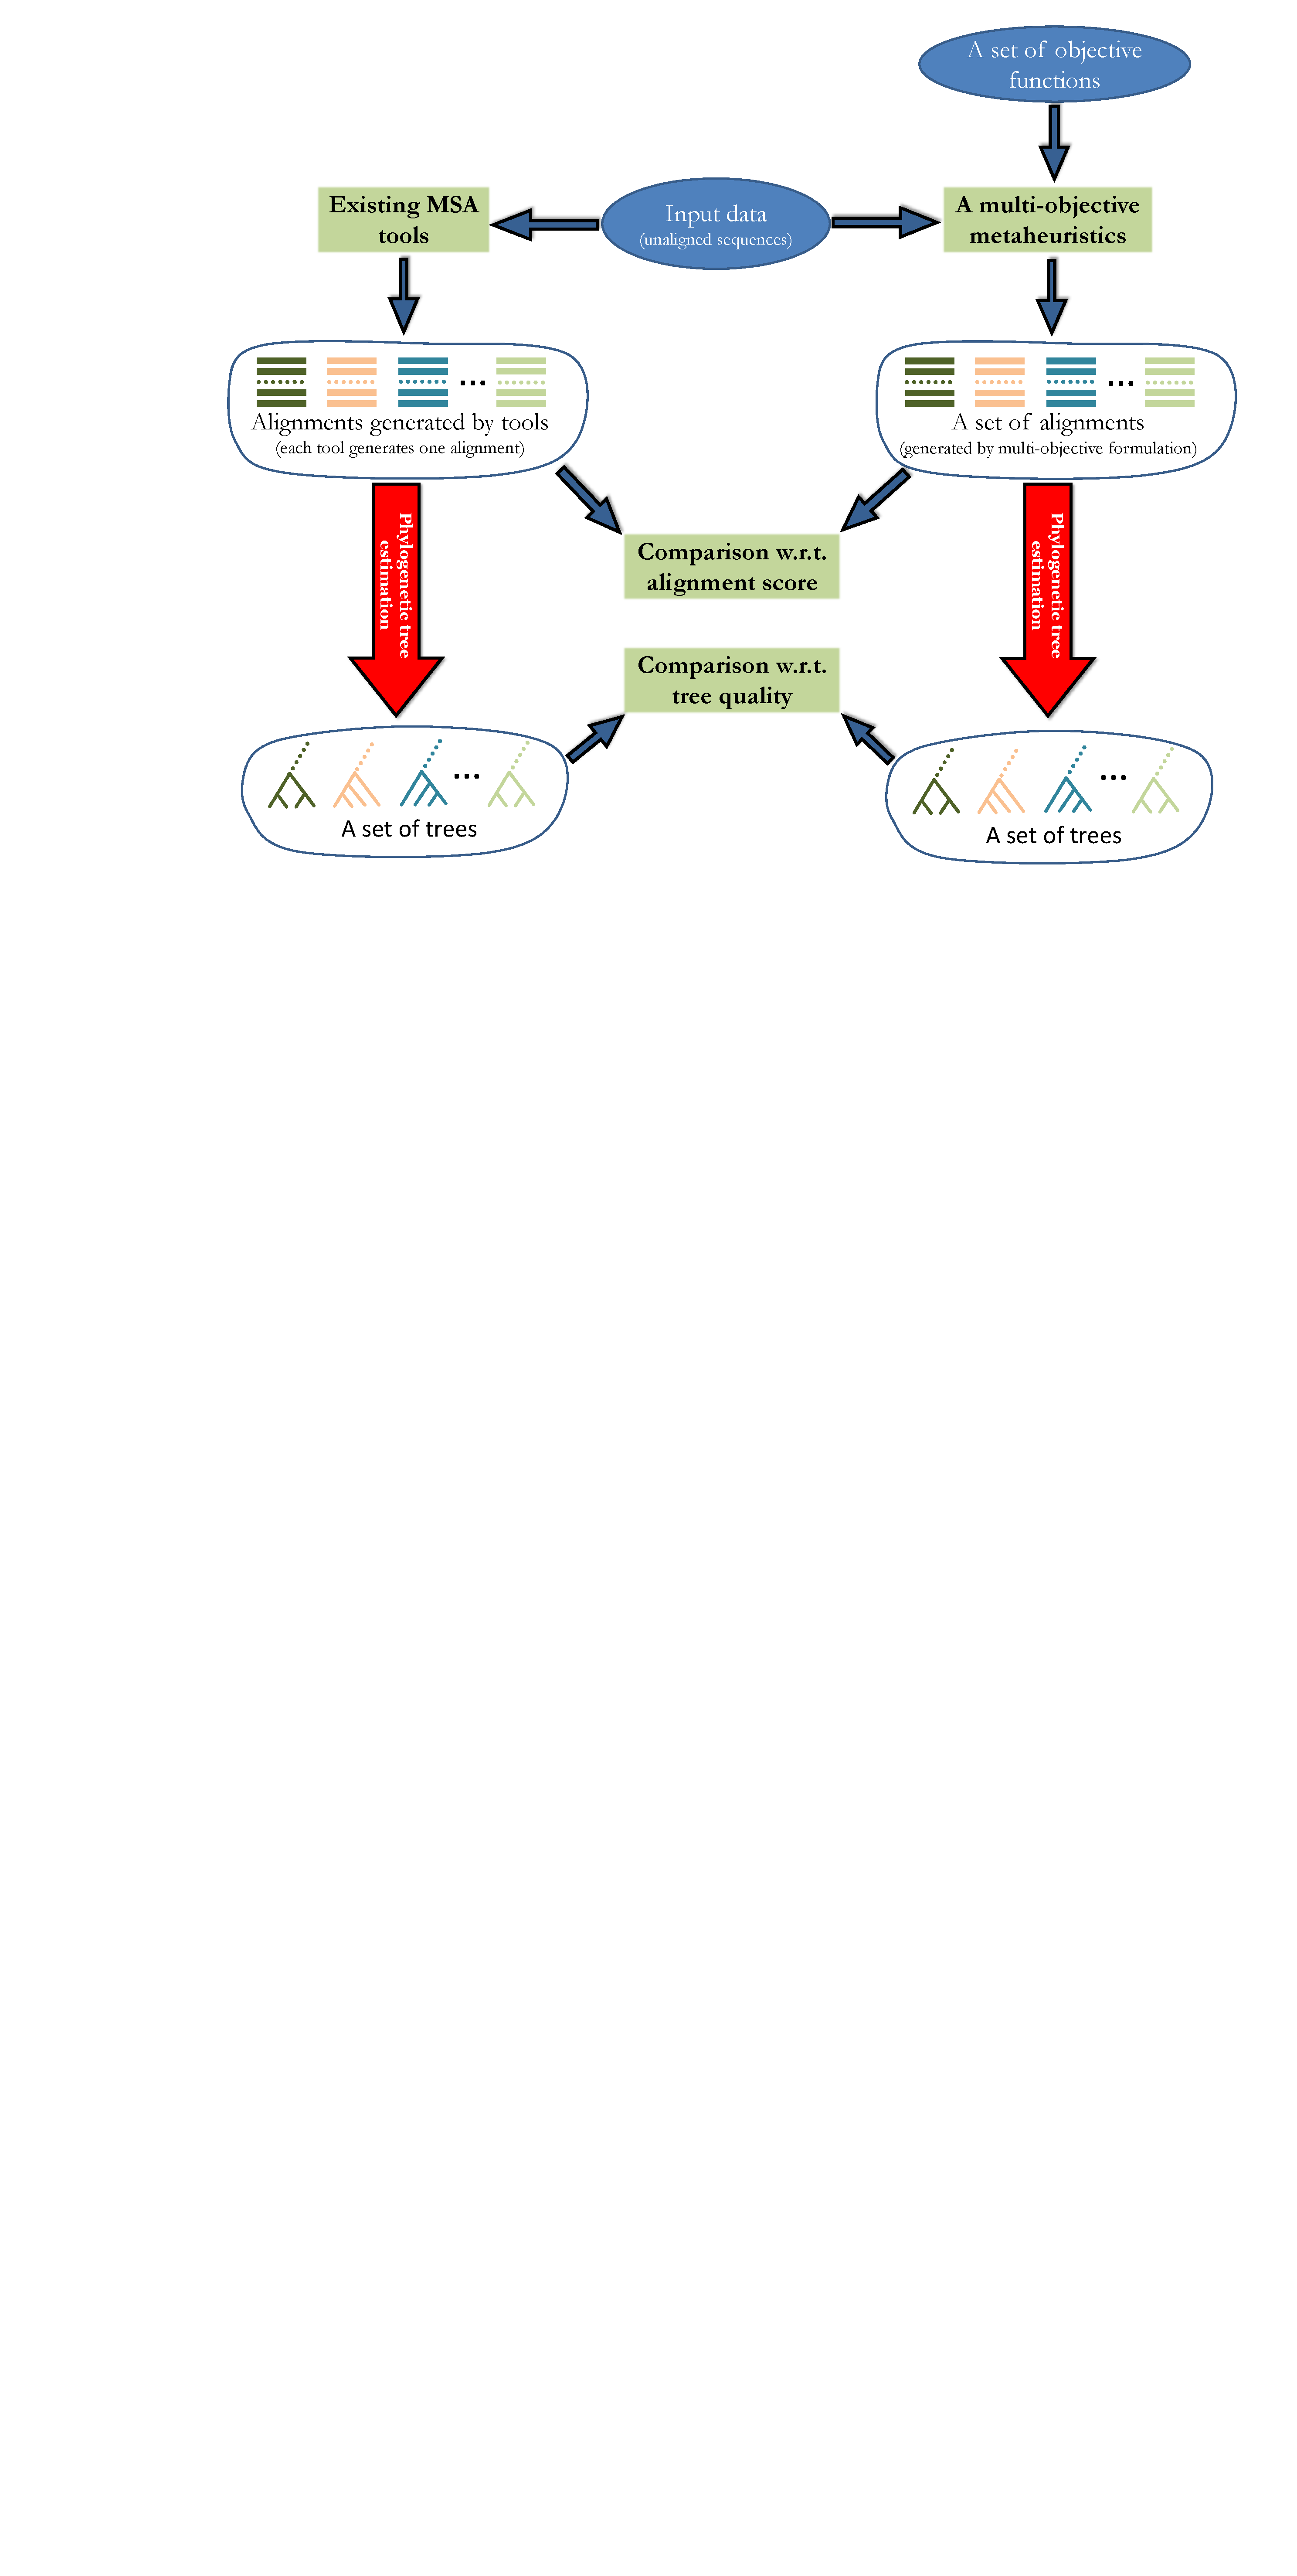
\includegraphics[width=0.8\textwidth]{Figure/pipeline}
	\caption[Our methodology for finding the impact of a multi-objective formulation of MSA on phylogenetic tree estimation.]{Our methodology for finding the impact of a multi-objective formulation (i.e., a set of objective functions) of MSA on phylogenetic tree estimation. For each dataset (i.e., unaligned sequences), we run a multi-objective metaheuristic. It simultaneously optimizes the given objective functions and outputs a set of alignments which represents the best-possible compromise among all objective functions. We also run several existing MSA tools on that dataset and each tool generates one alignment. We evaluate the quality of each generated alignments with respect to the reference alignments using widely used scores. Also, we estimate phylogenetic trees for all alignments and evaluate each tree with respect to the reference. Then we compare the alignments and the corresponding phylogenetic trees generated by the multi-objective formulation with the ones generated by the existing tools based on alignment score as well as tree quality. We also observe the association between alignment scores and tree quality values to examine whether it is appropriate to use alignment score in the context of phylogeny estimation.}
	\label{fig:pipeline}

\end{figure}

\subsection{Experiment settings}
\label{sec:exp_settings}
We summarize our experimental methodology (also illustrated in Figure~\ref{fig:pipeline}) in six steps as follows.
\begin{itemize}
	\item \underline{Step 1:} We identify and choose two bi-objective formulations, effective for phylogeny estimation, by adopting a systematic method incorporating multivariate linear regression analysis with the help of a simulated dataset. \item \underline{Step 2:} We optimize each bi-objective formulation selected in Step 1 by
	 running an appropriate MO metaheuristics on biological datasets. Each run outputs some competitive alignments. 
	\item \underline{Step 3:} Several existing MSA methods are also executed on all these datasets. Each method generates one alignment per dataset.
\item \underline{Step 4:} Based on two measures (i.e., SP and TC scores), that are very popular in the literature, we assess the goodness of all estimated alignments. \item \underline{Step 5:} Employing a standard approach, we infer the phylogenetic tree from every generated alignment. For each of the estimated trees, we assess the goodness thereof in terms of a well-known metric, namely, FN (false negative) Rate~\citep{warnow2017computational}.
	\item \underline{Step 6:} At last, we carefully compare the alignments along with their respective phylogenetic trees generated by the MO approach against those obtained from existing MSA tools. \end{itemize}
\subsection{Objective functions}
\label{sec:formulation}
Most of the real-life optimization problems actually aim to achieve multiple objectives, where objectives are (usually) in conflict with one another. An MO formulation enables us to optimize each objective independently. We select the following three formulations, for this thesis, considering their simplicity and effectiveness. \begin{itemize}
	\item \textit{\{SOP, TC\} formulation~\citep{da2010alineaga}:} Here, the sum of pairs score (i.e., SOP) and the totally aligned columns (i.e., TC) are maximized. 

	\item \textit{\{Gap, SOP\} formulation~\citep{abbasi2015local}:} Here, SOP is maximized and the number of gaps (i.e., Gap) is minimized.
	
	\item \textit{\{wSOP, TC\} formulation~\citep{rubio2016hybrid}:} Here, wSOP, i.e., the weighted sum of pairs with affine gap penalties and TC are maximized.
\end{itemize}

These objective functions with examples have been discussed in the supplementary file (please check Section~\ref{sec:objective _function}). Here  four new objective functions are proposed in the context of an MSA, which quantify different aspects thereof. We deliberately do not combine multiple aspects of an MSA into a single objective, unlike the approach taken predominantly in the literature. We introduce these four new objective functions as follows: 

\begin{itemize}
	\item \textbf{Minimizing entropy (Entropy)}: Contrary to the usual definition, we consider only non-gap columns for the calculation of entropy.
	
	\item \textbf{Maximizing similarity based on gap containing columns (SimG)}: Here, similarity is calculated only for the columns containing one or more gaps. 
	
	\item \textbf{Maximizing similarity based on non-gap columns (SimNG)}: Here, similarity is calculated only for the columns containing no gap.	
	\item \textbf{Maximizing concentration of gaps (GapCon)}: For each sequence, we count the consecutive gaps and take the mean of these counts. Finally, we average the resultant means for all sequences and use that as the Concentration of gaps.
	
\end{itemize}
At this point a brief discussion on the motivation behind proposing the fourth objective is order. Affine gap penalty~\citep{rani2016multiple} is a widely used objective function that combines (using weighted sum) two aspects of an aligned sequence, namely, the concentration and the number of gaps. Thus, one would need to tune the weight values based on the dataset. To avoid this we decouple the two components/aspects. Notably, the number of gaps (i.e., Gap) has already been considered by us as an objective function. 


From onward, the objectives discussed above are denoted by the acronyms listed in Table~\ref{tab:abbr} . 
\begin{table}[!htbp]
	\centering
\caption{Acronyms used for the optimization objectives.}
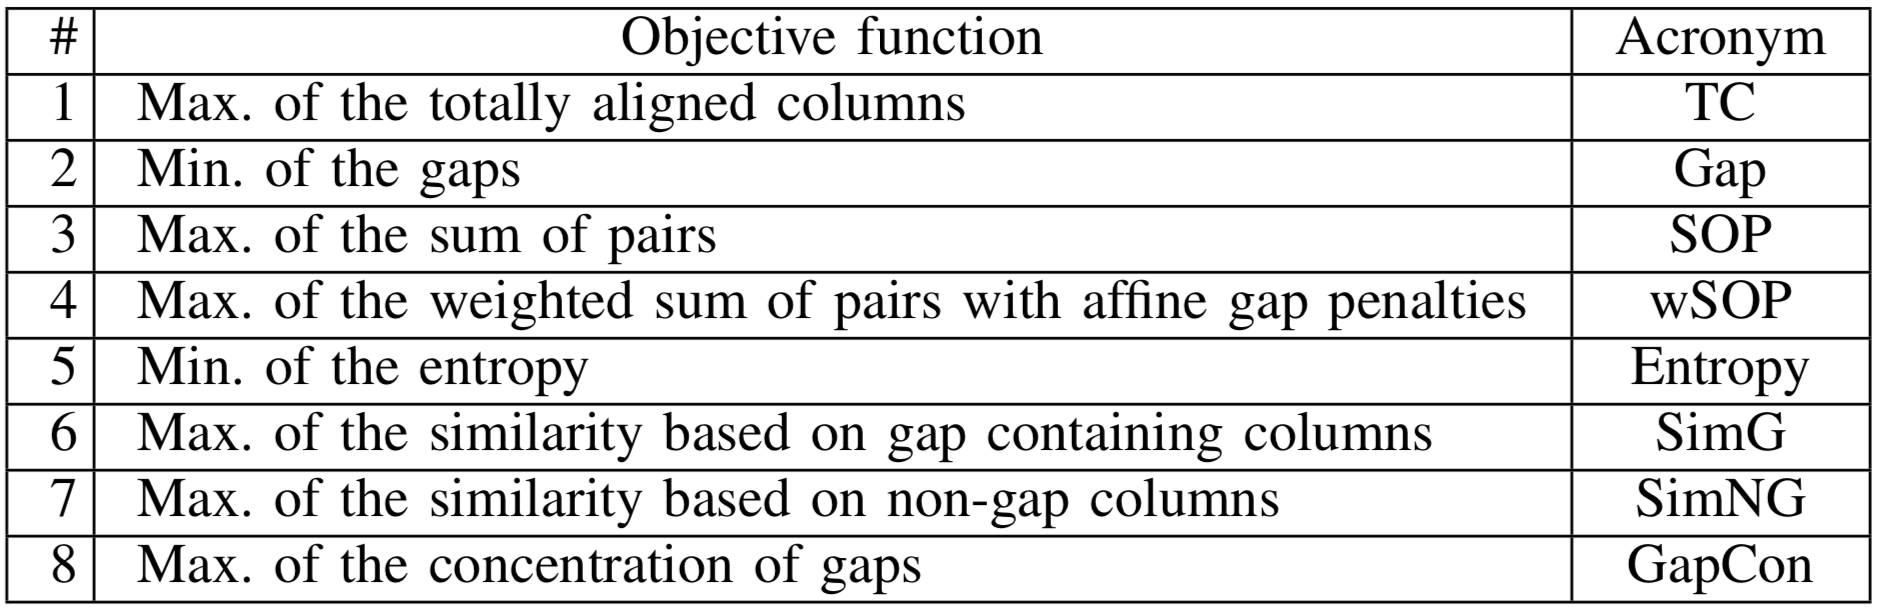
\includegraphics[width=0.8\columnwidth]{Figure/objective_acronym}
	\label{tab:abbr}
\end{table}

To evaluate SOP and wSOP, a substitution matrix is needed which depends on dataset characteristics. We have employed NUC4.4 and BLOSUM62 (available at ftp://ftp.ncbi.nih.gov/blast/matrices) for nucleotide and protein sequences, respectively. Informatively, all four objective functions we have proposed above are nonparametric.\subsection{MO metaheuristics}
We utilize three well-known MO metaheuristics: NSGA-II~\citep{deb2002fast}, NSGA-III~\citep{deb2014evolutionary} and MOEA/D~\citep{zhang2007moea}. They belong to the class of MO evolutionary algorithms. They start from a set of candidate solutions (termed as population) and then mimics concepts of natural evolution (such as mutation, crossover, selection, etc.) to evolve the population towards the optimal solutions. Unlike single-objective optimization methods, they output a lot of solutions (i.e., members of the final population) which is a compromise among all objectives in the best possible way. Three studies (\citep{zambrano2017m2align, ortuno2013optimizing, zambrano2017comparing}) demonstrated the superiority of NSGA-II to compute MSAs. NSGA-II can effectively tackle problems with upto three objectives whereas NSGA-III is developed in a particular way to handle more than three objectives. Keeping these in minds, we apply them according to Table~\ref{tab:variants}. We run MOEA/D, studied by~\cite{zhu2015novel} for MSA, with one formulation to compare its performance against NSGA-II.
These methods along with important parameters thereof are described in Section~\ref{sec:mop} (of the supplementary file). Besides, a short description of their vital components as follows. 
\begin{itemize}
	\item We used the encoding scheme proposed by~\cite{rubio2016hybrid} which stores each sequence as $[(b_1, e_1),$ $(b_2, e_2), ..., (b_n, e_n)]$, where $(b_i, e_i)$ represents the begin and end position of a group of consecutive gaps in the sequence. \cite{zambrano2017m2align} studied the benefit of such encoding over the traditional binary representation.
	
	\item As mutation operator, we used closed gap shifting~\cite{ortuno2013optimizing}, which randomly chooses consecutive gaps from a sequence and shifts to another random position. This shifting may result in columns having only gaps which are then removed. Thus, in effect, it tries to remove gaps from the MSA. 
	
	\item The crossover operator~\citealp{da2010alineaga} acts as a single-point crossover on two parent alignments (let us refer to them as $ P1 $ and $ P2 $). It picks a random column from P1 to break it into two segments: $ P1^L $ and $ P1^R $. The selected column elements are located in P2 (which are not necessarily belongs to the same column) and used to cut P2 into two segments: $ P2^L $ and $ P2^R $. Then, the generated segments are interchanged between these two parents to create two offspring alignments: [$P1^L + P2^R$] and [$P2^L + P1^R$]. At the end, gaps are used to fill the empty cells (if any) appeared at the junction.
\end{itemize}

We implemented the above two metaheuristics using jMetalMSA~\citep{zambrano2017multi} which is a Java metaheuristic framework for MSA. The important parameters with corresponding values are listed in Table~\ref{tab:parameters}. We adopt the same mutation and crossover operator, along with the associated parameter values, used by~\cite{ortuno2013optimizing}.  

\begin{comment}
We provide a short description of these operators below. 
%publicly available at~\url{https://github.com/jMetal/jMetalMSA}. 

\begin{itemize}

\item The mutation operator is termed as closed gap shifting, where consecutive gaps are randomly chosen and shifted to another random position in a sequence. This shifting may result columns having only gaps which are then removed. Thus this mutation tries to reduce the number of gaps in the MSA. 

\item The crossover operator is the single-point crossover over alignments proposed by~\citealp{da2010alineaga}. The operator randomly selects a column from one parent to split it into two blocks (let us refer to them P1a and P1b). The same selected positions are located in the other parent (which are not necessarily in the same column) and is tailored so that the right piece can be joined to the left piece of the first parent and vice versa (P2a and P2b). Finally, the selected blocks are exchanged between these two parents to create two new individuals with the combination of the blocks: [P1a + P2b] and [P1a + P1b]. After that, any empty space that appears at the junction point is filled with gaps.
%NSGAIII has been shown to perform reasonably on handling a large number of objective functions~\cite{deb2014evolutionary}.	
\end{itemize}
\end{comment}

% Table generated by Excel2LaTeX from sheet 'param'
\begin{table}[!htbp]
	\centering
	\small
	\caption{Major parameters of our algorithms.}
	\begin{tabular}{|c|c|c|} %|c|C{3cm}|C{3.2cm}|
		\hline
		Algo. & \multicolumn{1}{c|}{Parameter} & Value \\
		\hline
		\multirow{5}{*}{All} & Max. generations & 500 \\
		
		\cline{2-3}          & Mutation  & Closed gap shifting \\
		\cline{2-3}          & Mutation rate & 0.2 \\
		\cline{2-3}          & Crossover  & Single-point crossover \\
		\cline{2-3}          & Crossover rate & 0.8 \\ %, $C_r$
		\hline
		\multirow{2}{*}{NSGA-II} & Population size & 100 \\ %, $\overline{N}$
		\cline{2-3}          & No. of runs & 20 \\
		\hline
		\multirow{3}{*}{NSGA-III} & No. of reference points & 120 \\
		\cline{2-3}          & Population size & 120 (78) \\ %, $N$
		\cline{2-3}          & No. of runs & 25 (40) \\
		\hline
		\multirow{2}{*}{MOEA/D} & Population size & 100 \\ %, $\overline{N}$
		\cline{2-3}          & No. of runs & 20 \\
		\cline{2-3}          & Neighborhood size & 10 \\
		\cline{2-3}          & Aggregation function & Tchebycheff approach \\
		\hline
	\end{tabular}%
	\label{tab:parameters}%
\end{table}%

\begin{table}[!htbp]
\centering
	\caption{Selected multi-objective (MO) metaheuristics.}
	\begin{tabular}{|c|l|} \hline
		Algorithm & Objective set to optimize \\
		\hline
		\multicolumn{1}{|c|}{\multirow{2}{*}{NSGA-II}} & \{wSOP, TC\}, 
		\{SOP, TC\},          \\
		& \{Gap, SOP\},
		\{SimG, SimNG\} \\
		\hline
		\multicolumn{1}{|c|}{\multirow{2}{*}{NSGA-III}} & \{wSOP, Gap, TC, SOP\} \\
		& \{SimNG, SimG, GapCon, Entropy, TC, Gap\} \\
		\hline
		\multicolumn{1}{|c|}{\multirow{1}{*}{MOEA/D}} & \{SimNG, SimG\}\\
		\hline
	\end{tabular}\label{tab:variants}\end{table}These algorithms have been implemented using an open-source framework, jMetalMSA (\url{https://github.com/jmetal/jmetalmsa}). We have made our source code available at \url{https://github.com/ali-nayeem/MSA}.\subsection{State-of-the-art MSA tools}
 We use nine representative MSA tools (listed in Table~\ref{tab:msa_tools}) in our experimental study. Each of them is invoked with the default parameter settings. Moreover, we randomly generate the initial population of our chosen metaheuristics by mixing and modifying the alignments generated by these tools. \begin{table}[htbp]
\centering
	\caption{ Existing MSA tools used for experimentation.}
	\begin{tabular}{|l|l||l|l|}
		\hline
		\multicolumn{2}{|c||}{For nucleotide sequences} & \multicolumn{2}{c|}{For protein sequences} \\
		\hline
		\multicolumn{1}{|c|}{Tool} & \multicolumn{1}{c||}{Version} & \multicolumn{1}{c|}{Tool} & \multicolumn{1}{c|}{Version} \\
		\hline
		FSA~\citep{bradley2009fast} & 1.15.9 & FSA   & 1.15.9 \\
		\hline
		PASTA~\citep{mirarab2015pasta} & 1.7.8 & PASTA & 1.7.8 \\
		\hline
		T-Coffee~\citep{notredame2000t} & 11.00 & T-Coffee & 11.00 \\
		\hline
		MAFFT~\citep{katoh2002mafft} & 7.31  & MAFFT & 7.245 \\
		\hline
		Clustal W~\citep{thompson1994clustal} & 2.1   & Clustal W & 2.1 \\
		\hline
		Clustal $ \Omega $~\citep{sievers2011fast} & 1.2.4 & RetAlign~\citep{szabo2010reticular} & 1.0 \\
		\hline
		MUSCLE~\citep{edgar2004muscle} & 3.8.31 & MUSCLE & 3.8.31 \\
		\hline
		PRANK~\citep{loytynoja2005algorithm} & 0.170427 & ProbCons~\citep{do2005probcons} & 1.12 \\
		\hline
		Kalign~\citep{lassmann2008kalign2} & 2.03  & Kalign & 2.04 \\
		\hline
	\end{tabular}\label{tab:msa_tools}\end{table}\subsection{Evaluation of estimated alignments}
\label{sec:msa_eval}
We evaluate estimated alignments using two widely known alignment quality measures: SP and TC scores. They compare the estimated alignment (output) to the reference alignment (reference) in two different ways: the former expresses the ratio of aligned columns recovered in the output with respect to the aligned columns present in the reference, whereas the latter shows the ratio of aligned pairs. 
A higher value implies better score for both of them.\subsection{Estimating Phylogenetic trees}
\label{sec:tree_estimation}
For each generated alignment, we generate the phylogenetic tree. To do so, we use a the standard way of estimating phylogenetic trees from sequence data, i.e., the Maximum Likelihood  method~\cite{liu2011raxml}. FastTree\citep{price2010fasttree} and RAxML~\citep{stamatakis2014raxml} are the most widely used software for this purpose. FastTree can produce output very quickly with negligible difference in tree accuracy compared to RAxML~\cite{liu2011raxml}. In this thesis we had to estimate numerous phylogenetic trees. So we prefer FastTree over RAxML.\subsection{Evaluating phylogenetic trees}
\label{sec:tree_eval}
We assess and evaluate each of the estimated phylogenetic trees based on the FN Rate against the true phylogenetic tree. 
FN rate actually expresses (in percentage) the fraction of edges that exist in the latter (i.e., in true tree) but are absent in the former (i.e., in the estimated one). Clearly, the smaller the value of FN rate, the more desirable it is. Although there are two more common tree error measures (False Positive (FP rate) and and Robinson-Foulds (RF) rate), all of them are identical when true and estimated trees are binary~\citep{warnow2017computational}. In this thesis we worked with binary trees only.\subsection{Evaluation of an objective function}
\label{sec:obj_eval}
An MSA objective function should be considered desirable in the context of phylogeny inference only if alignments generated using such objective functions lead to highly accurate phylogenetic trees (i.e., the generate trees exhibit low FN rates).     
Therefore, in an attempt to assess the effectiveness of an objective function we examine how the values thereof are associated with the values of respective FN rates. An objective function is predicted to be a good optimization criteria in our context only if it frequently exhibits positive correlation with FN rate of the trees estimated using the alignments generated by the MO algorithm (leveraging that objective function) for MSA.   
Therefore, in our approach, multivariate linear regression has been employed to estimate the above-mentioned correlation (i.e., regression coefficient) followed by an application of $t$-test (to check the significance of individual regression coefficients) with the null hypothesis that there is no association. While the above regression result may not conclusively indicate the suitability of an objective as an optimization criterion, the chosen objective functions through this methodology can definitely be utilized as potential candidates for further (empirical) validation.



 \section{Results}
\label{sec:results}
This section reports the results of our comprehensive experiments using our methodology and nine existing MSA tools listed in Table \ref{tab:msa_tools}. We start with describing our datasets. In what follows, the (best) results  of an existing MSA method/tool will indicate the results of the nine tools listed in Table \ref{tab:msa_tools}.


\subsection{Datasets}
To conduct our study, we used a simulated dataset (100-taxon simulated dataset~\citep{liu2009rapid}) as well as two biological datasets (biological rRNA datasets~\citep{liu2009rapid} and the BAliBASE 3.0 benchmark~\citep{thompson2005balibase}). The true phylogenetic tree provided with the simulated dataset enables us to analyze whether a MO formulation is potentially application-aware and subsequently we choose two such formulations (Section~\ref{sec:selection_msa_formulation}) which resemble the training period of a supervised learning method to some extent. Afterwards, we evaluate the efficacy of the chosen formulations using biological datasets with respect to the MSA tools listed in Table \ref{tab:msa_tools}.  


From the 100-taxon simulated dataset, we picked five random replicates. And among the biological datasets, we chose two challenging ribosomal RNA datasets along with 27 random BAliBASE instances. We describe these datasets in detail in the supplementary file (Section~\ref{sec:dataset_stat}). 

%\subsection{Dataset statistics}
%\label{sec:dataset_stat}
% Table generated by Excel2LaTeX from sheet 'Sheet1'
\subsubsection{100-taxon simulated dataset}
We used five randomly selected replicates (R0, R4, R9, R14, R19) of simulated nucleotide dataset from the study of~\citealp{liu2009rapid}. It is publicly available at \url{https://sites.google.com/eng.ucsd.edu/datasets/sate-i}. Table~\ref{tab:sim_stat} gives the reference alignment statistics for this dataset.

\begin{table}[htbp]
	\centering
	\caption{Reference alignments for 100-taxon simulated dataset.}
	\begin{tabular}{|l|r|}
		\hline
		\multicolumn{1}{|c|}{Feature} & \multicolumn{1}{c|}{Value} \\
		\hline
		Number of taxa & 100 \\
		\hline
		Number of sites & 1698.2 \\
		\hline
		Percent indels & 40.4 \\
		\hline
		Avg. gap length & 3.1 \\
		\hline
	\end{tabular}%
	\label{tab:sim_stat}%
\end{table}%


\subsubsection{Biological rRNA datasets}
We analyzed two biological ribosomal RNA datasets, 23S.E and 23S.E.aa\_ag, from~\citealp{liu2009rapid} which are challenging for phylogeny estimation methods. Each of these datasets is given with a highly reliable, curated reference alignment from Gutell Lab. The statistics of the reference alignments of these datasets are presented in Table~\ref{tab:bio_stat}. Reference trees for these datasets were generated from the reference alignments by running RAxML~\citep{stamatakis2014raxml} with bootstrapping, and retaining only the highly supported edges. We evaluated generated alignments with respect to the reference alignment using the tool FastSP \citep{mirarab2011fastsp}.
% Table generated by Excel2LaTeX from sheet 'Sheet2'
\begin{table}[htbp]
	\small
	\centering
	\caption{Reference alignments for two biological rRNA datasets.}
	\begin{tabular}{|l|r|r|}
		\hline
		\multicolumn{1}{|c|}{Feature} & \multicolumn{1}{c|}{23S.E.aa\_ag} & \multicolumn{1}{c|}{23S.E} \\
		\hline
		Number of taxa & 144   & 117 \\
		\hline
		Number of sites & 8,619 & 9,079 \\
		\hline
		Percent indels & 61.1  & 59.7 \\
		\hline
		Avg. gap length & 13.5  & 12.6 \\
		\hline
	\end{tabular}%
	\label{tab:bio_stat}%
\end{table}%

\subsubsection{BAliBASE datasets}\label{subsec:balibase_stat}
BAliBASE 3.0 \citep{thompson2005balibase} is the most widely used benchmark alignment databases of protein families. It provides manually refined reference alignments of high quality based on 3D structural superposition. These datasets are organized into six groups according to their families and similarities: RV11 (very divergent sequences, residue identity below 20\% ), RV12 (medium to divergent sequences, 20\%-40\% residue identity), RV20 (families with one or more highly divergent sequences), RV30 (divergent subfamilies), RV40 (sequences with large terminal N/C extensions), and RV50 (sequences with large internal insertions). In this chapter, we selected four to five representative datasets from each group as reported in Table~\ref{tab:balibase}. We generated reference trees for these datasets by running RAxML~\citep{stamatakis2014raxml} with bootstrapping. We evaluated estimated alignments with respect to the core blocks (regions for which reliable alignments are known to exist) using the program bali\_score available at~\url{http://www.lbgi.fr/balibase/BalibaseDownload/}.

% Table generated by Excel2LaTeX from sheet 'Sheet2'
\begin{table}[htbp]
	\small
	\centering
	\caption{ BAliBASE datasets selected for this chapter.}
	\begin{tabular}{|l|l|}
		\hline
		\multicolumn{1}{|c|}{Group} & \multicolumn{1}{c|}{Datasets selected} \\
		\hline
		RV11  & BB11005, BB11018, BB11020, BB11033 \\
		\hline
		RV12  & BB12001, BB12013, BB12022, BB12035, BB12044 \\
		\hline
		RV20  & BB20001, BB20010, BB20022, BB20033, BB20041 \\
		\hline
		RV30  & BB30002, BB30008, BB30015, BB30022 \\
		\hline
		RV40  & BB40001, BB40013, BB40025, BB40038, BB40048 \\ %
		\hline
		RV50  & BB50001, BB50005, BB50010, BB50016 \\
		\hline
	\end{tabular}%
	\label{tab:balibase}%
\end{table}%

\subsection{Selection of appropriate MO formulations}
\label{sec:selection_msa_formulation}
As we stated above, our simulated dataset is used to find out potentially ``application-aware'' MO formulation(s). Through extensive experimentation, We first choose a bi-objective formulation from among three popular MO formulations found in the literature (see Section \ref{sec:methods}). Subsequently, we propose a new promising bi-objective formulation from among four objectives proposed in this chapter (see Section \ref{sec:methods}). In each case, we follow a systematic approach based on two criteria: (1) the selected two objectives should be conflicting to each other, (2) the selected objectives should exhibit a relatively good association with the FN rate. Note that, criterion (1) makes the employment of an MO algorithm more attractive as a compromise between two conflicting objectives increases the diversity of generated solutions. 
\begin{comment}
\begin{figure*}[!htbp]    
\begin{adjustwidth}{-1cm}{-1cm}
\centering
\begin{subfigure}{0.35\textwidth}
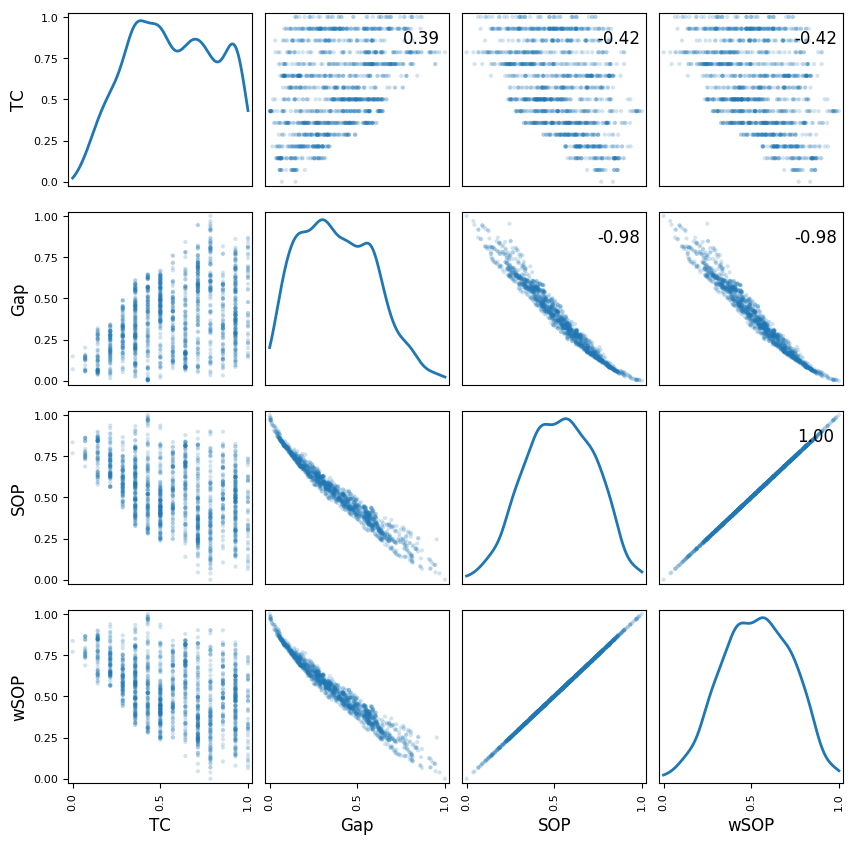
\includegraphics[width=\columnwidth]{Figure/NumGaps_SOP_TC_wSOP/precomputedInit/R0/fig/scatter_mattrix}
\caption{R0}
\end{subfigure}    
\begin{subfigure}{0.35\textwidth}
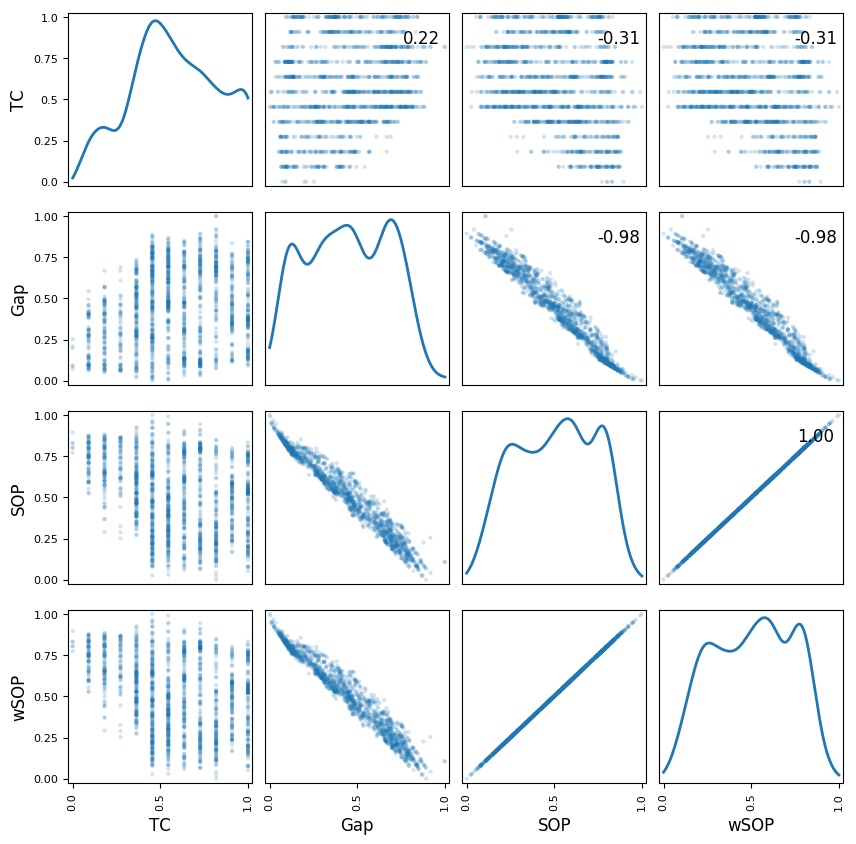
\includegraphics[width=\columnwidth]{Figure/NumGaps_SOP_TC_wSOP/precomputedInit/R4/fig/scatter_mattrix}
\caption{R4}
\end{subfigure}
\begin{subfigure}{0.35\textwidth}
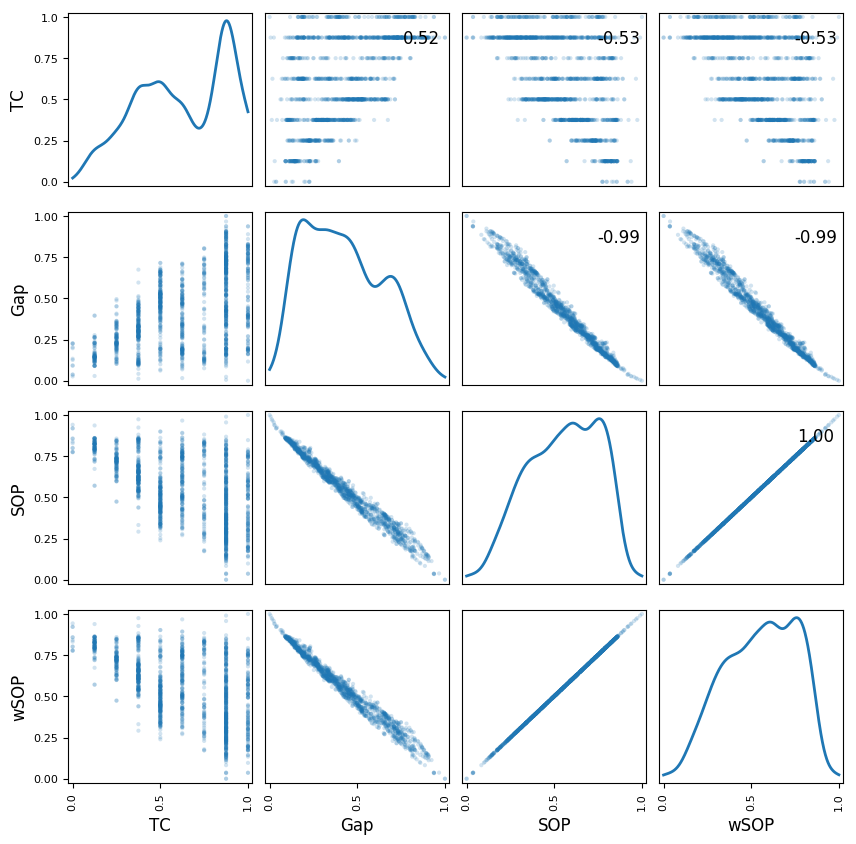
\includegraphics[width=\columnwidth]{Figure/NumGaps_SOP_TC_wSOP/precomputedInit/R9/fig/scatter_mattrix}
\caption{R9}
\end{subfigure}
\begin{subfigure}{0.35\textwidth}
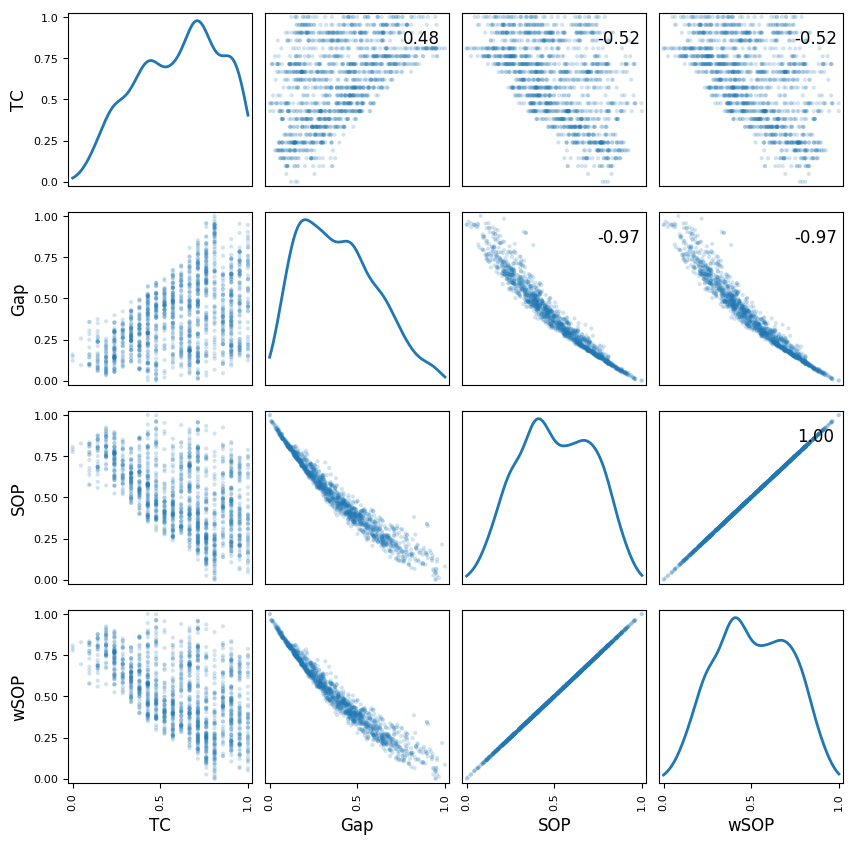
\includegraphics[width=\columnwidth]{Figure/NumGaps_SOP_TC_wSOP/precomputedInit/R14/fig/scatter_mattrix}
\caption{R14}
\end{subfigure}
\begin{subfigure}{0.35\textwidth}
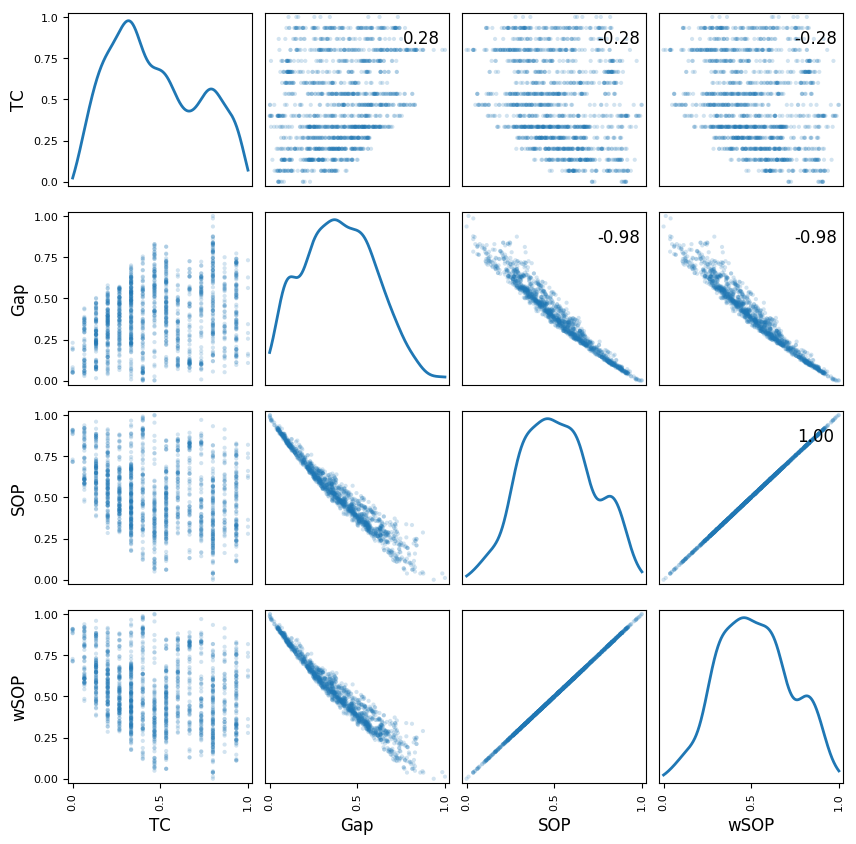
\includegraphics[width=\columnwidth]{Figure/NumGaps_SOP_TC_wSOP/precomputedInit/R19/fig/scatter_mattrix}
\caption{R19}
\end{subfigure}
\caption{\underline{100-taxon simulated dataset:} Scatter-plot matrices depicting the pairwise relationship of all objective functions on five randomly selected replicates. We turn each objective function into minimization form and then normalize using min-max technique. In each matrix, the diagonal cells show the distribution of objective values (estimated using KDE) while the non-diagonal cells show the correlation between pairs of objective functions. Each upper-diagonal cell contains the value of correlation coefficient $r$ of the corresponding pair of objective functions.}
\label{fig:nature_obj}
\end{adjustwidth}
\end{figure*}

\begin{figure*}[!htbp]
\centering
\small
\begin{adjustwidth}{-1cm}{-1cm}
\begin{tabular}{l||C{0.24\textwidth}|C{0.24\textwidth}|C{0.24\textwidth}|C{0.24\textwidth} }
& TC & Gap & SOP & wSOP\\\hline\hline
\rotatebox[origin=c]{-90}{R0} & 
\raisebox{-.5\height}{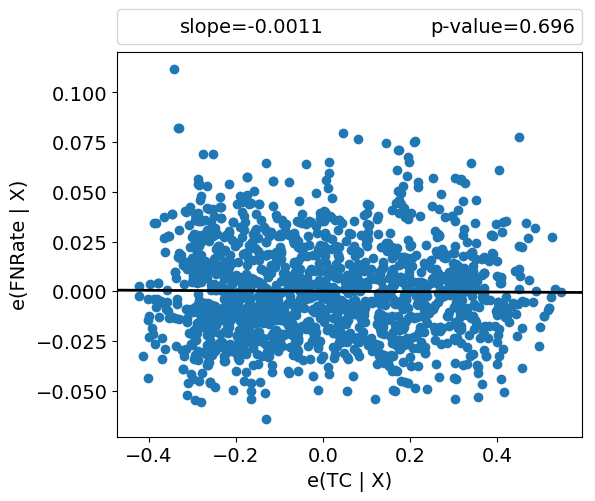
\includegraphics[width=0.25\textwidth]{Figure/NumGaps_SOP_TC_wSOP/precomputedInit/R0/fig/tc_partial_regression}} &
\raisebox{-.5\height}{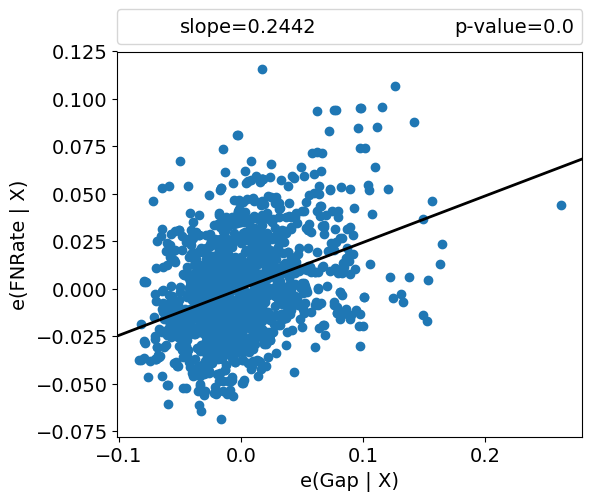
\includegraphics[width=0.25\textwidth]{Figure/NumGaps_SOP_TC_wSOP/precomputedInit/R0/fig/gap_partial_regression}} & 
\raisebox{-.5\height}{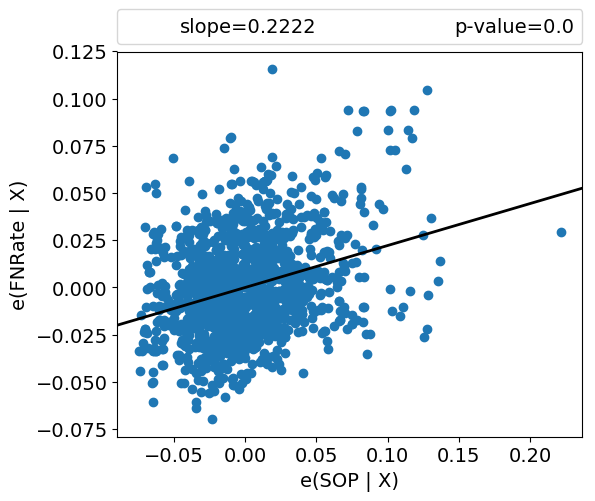
\includegraphics[width=0.25\textwidth]{Figure/NumGaps_SOP_TC_wSOP/precomputedInit/R0/fig/sop_partial_regression}} & 
\raisebox{-.5\height}{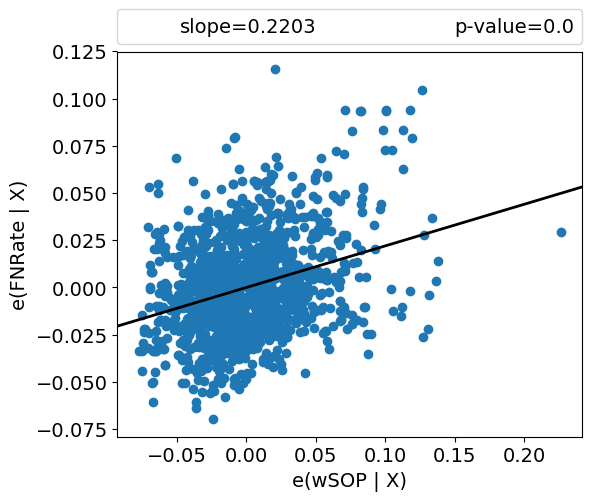
\includegraphics[width=0.25\textwidth]{Figure/NumGaps_SOP_TC_wSOP/precomputedInit/R0/fig/wsop_partial_regression}}     
\\\hline
\rotatebox[origin=c]{-90}{R4} &
\raisebox{-.5\height}{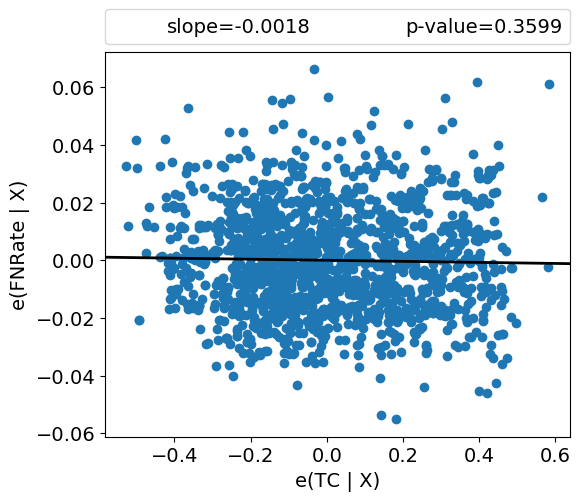
\includegraphics[width=0.25\textwidth]{Figure/NumGaps_SOP_TC_wSOP/precomputedInit/R4/fig/tc_partial_regression}} &
\raisebox{-.5\height}{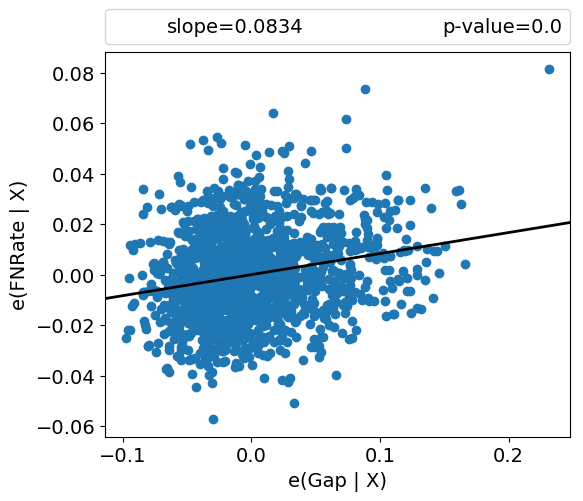
\includegraphics[width=0.25\textwidth]{Figure/NumGaps_SOP_TC_wSOP/precomputedInit/R4/fig/gap_partial_regression}} & 
\raisebox{-.5\height}{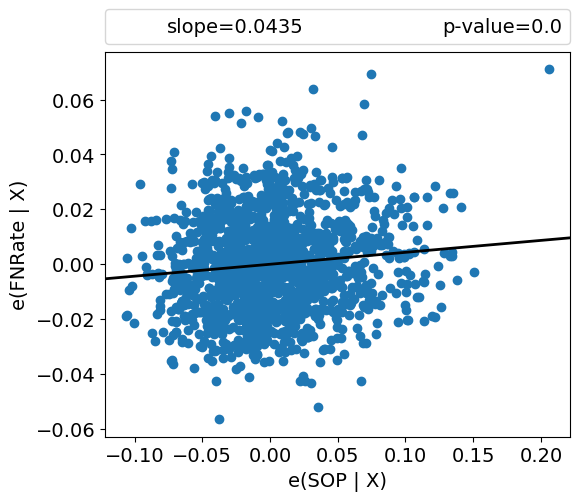
\includegraphics[width=0.25\textwidth]{Figure/NumGaps_SOP_TC_wSOP/precomputedInit/R4/fig/sop_partial_regression}} & 
\raisebox{-.5\height}{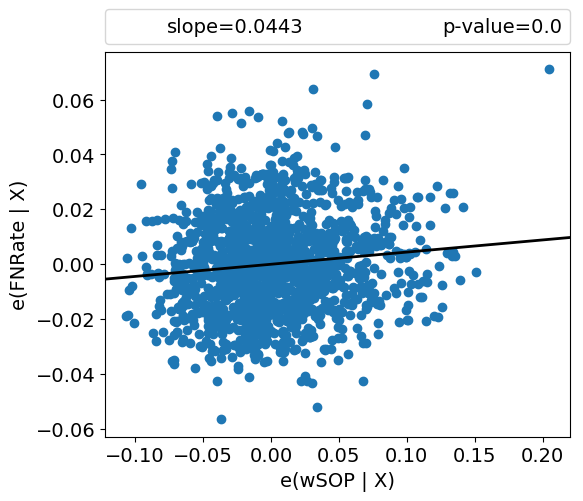
\includegraphics[width=0.25\textwidth]{Figure/NumGaps_SOP_TC_wSOP/precomputedInit/R4/fig/wsop_partial_regression}}
\\\hline
\rotatebox[origin=c]{-90}{R9} &
\raisebox{-.5\height}{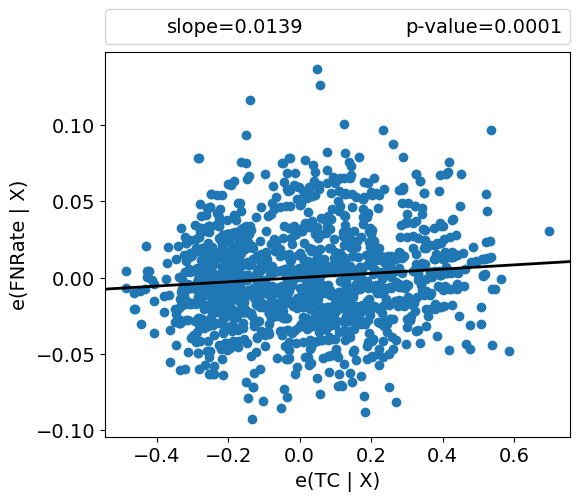
\includegraphics[width=0.25\textwidth]{Figure/NumGaps_SOP_TC_wSOP/precomputedInit/R9/fig/tc_partial_regression}} &
\raisebox{-.5\height}{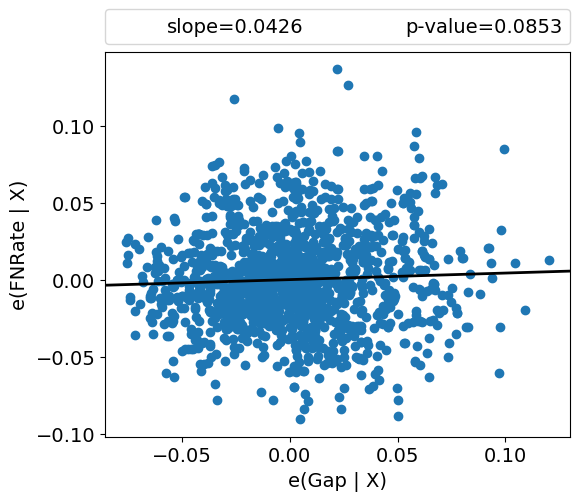
\includegraphics[width=0.25\textwidth]{Figure/NumGaps_SOP_TC_wSOP/precomputedInit/R9/fig/gap_partial_regression}} & 
\raisebox{-.5\height}{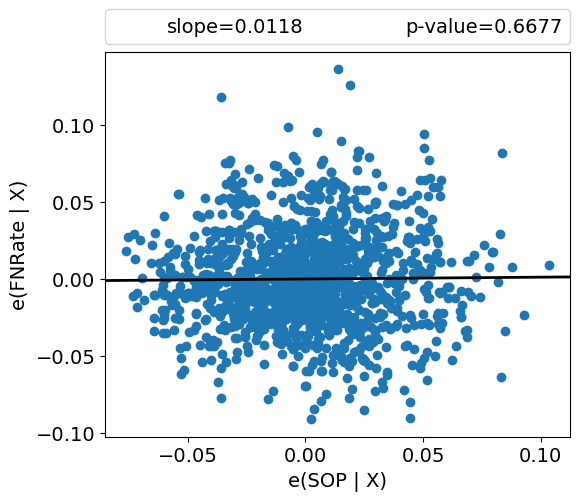
\includegraphics[width=0.25\textwidth]{Figure/NumGaps_SOP_TC_wSOP/precomputedInit/R9/fig/sop_partial_regression}} & 
\raisebox{-.5\height}{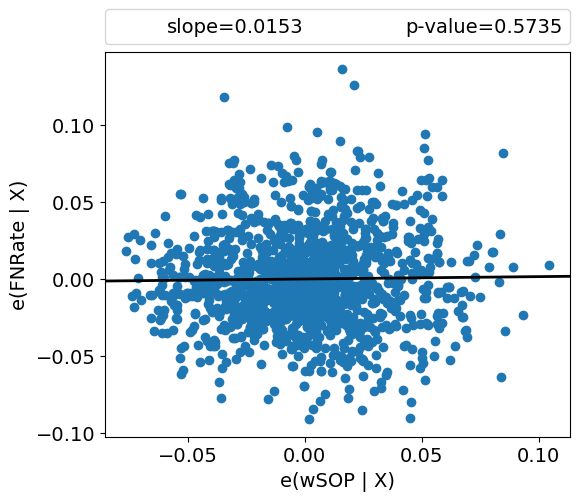
\includegraphics[width=0.25\textwidth]{Figure/NumGaps_SOP_TC_wSOP/precomputedInit/R9/fig/wsop_partial_regression}}
\\\hline
\rotatebox[origin=c]{-90}{R14} &
\raisebox{-.5\height}{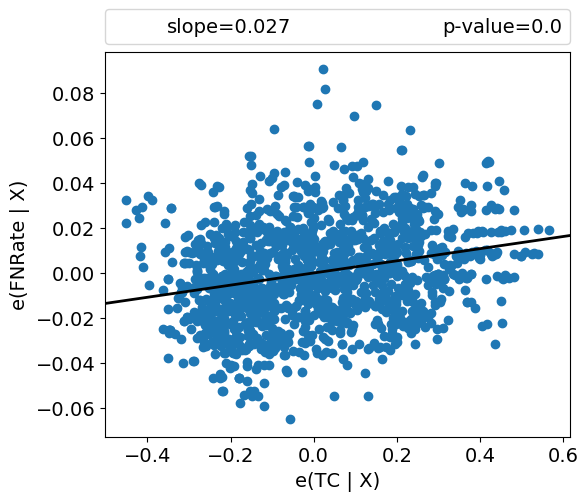
\includegraphics[width=0.25\textwidth]{Figure/NumGaps_SOP_TC_wSOP/precomputedInit/R14/fig/tc_partial_regression}} &
\raisebox{-.5\height}{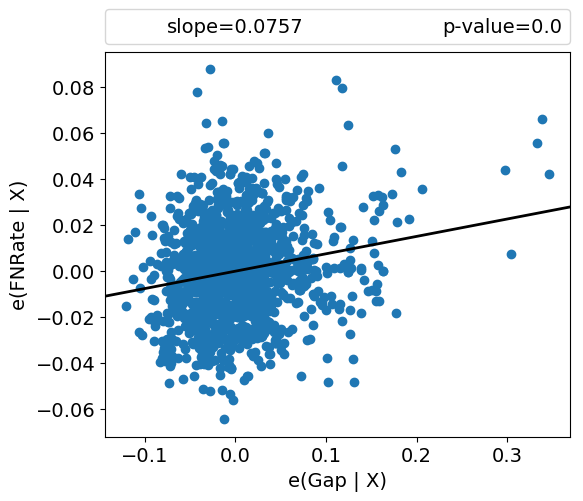
\includegraphics[width=0.25\textwidth]{Figure/NumGaps_SOP_TC_wSOP/precomputedInit/R14/fig/gap_partial_regression}} & 
\raisebox{-.5\height}{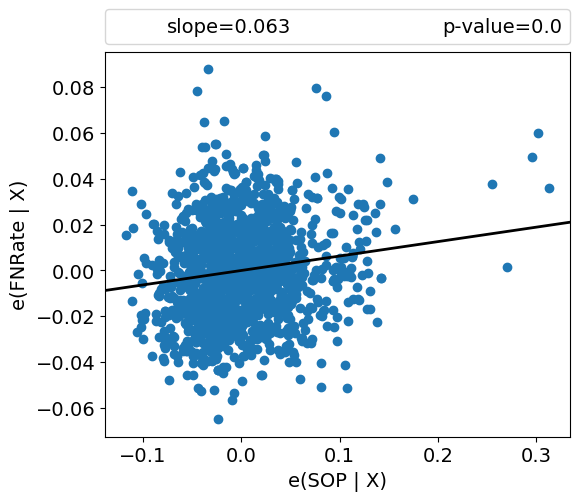
\includegraphics[width=0.25\textwidth]{Figure/NumGaps_SOP_TC_wSOP/precomputedInit/R14/fig/sop_partial_regression}} & 
\raisebox{-.5\height}{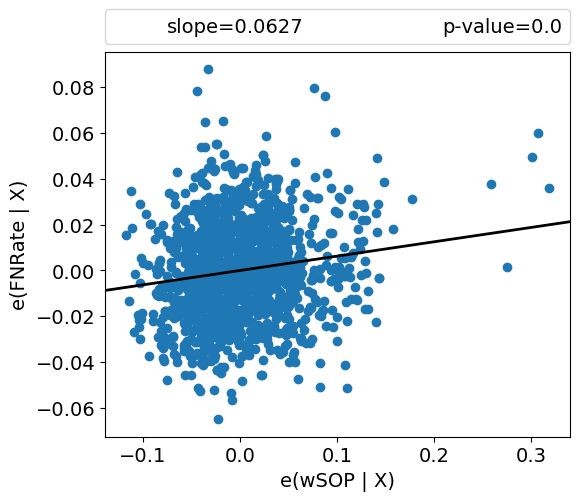
\includegraphics[width=0.25\textwidth]{Figure/NumGaps_SOP_TC_wSOP/precomputedInit/R14/fig/wsop_partial_regression}}
\\\hline
\rotatebox[origin=c]{-90}{R19} &
\raisebox{-.5\height}{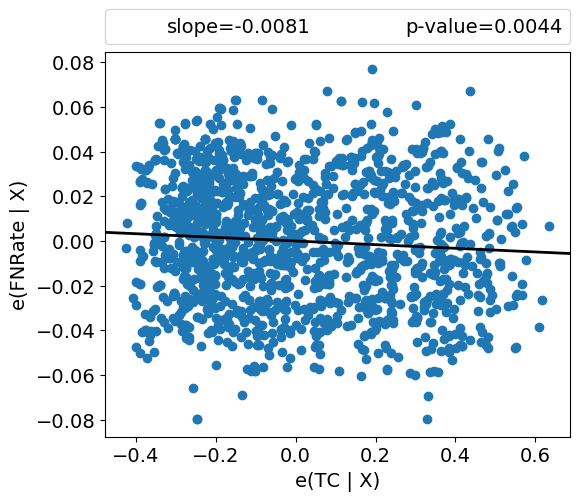
\includegraphics[width=0.25\textwidth]{Figure/NumGaps_SOP_TC_wSOP/precomputedInit/R19/fig/tc_partial_regression}} &
\raisebox{-.5\height}{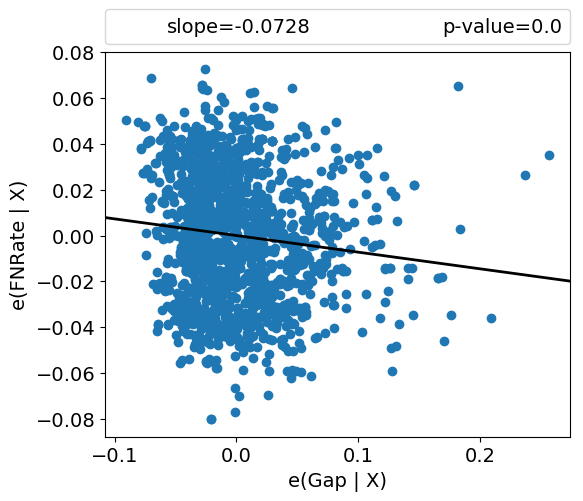
\includegraphics[width=0.25\textwidth]{Figure/NumGaps_SOP_TC_wSOP/precomputedInit/R19/fig/gap_partial_regression}} & 
\raisebox{-.5\height}{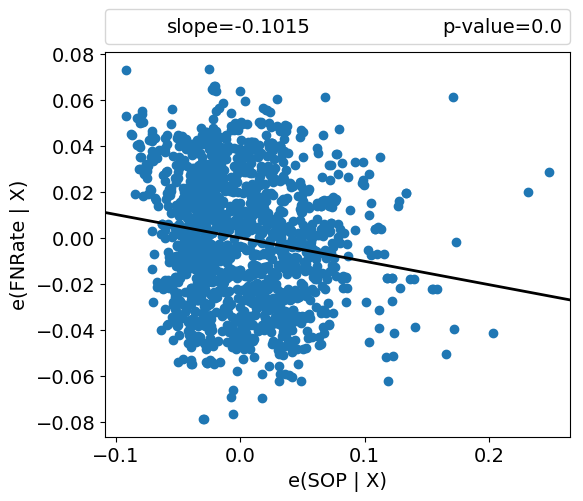
\includegraphics[width=0.25\textwidth]{Figure/NumGaps_SOP_TC_wSOP/precomputedInit/R19/fig/sop_partial_regression}} & 
\raisebox{-.5\height}{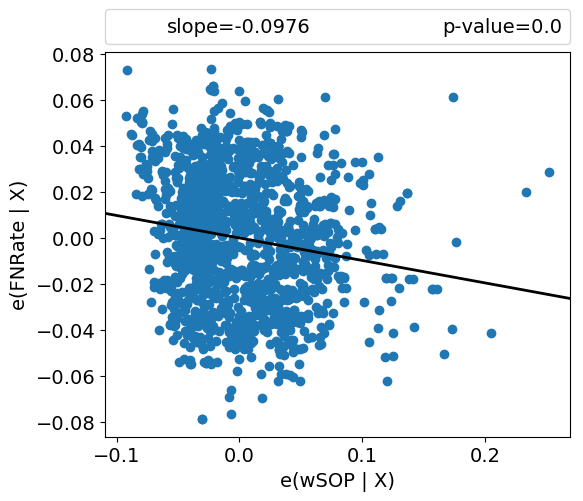
\includegraphics[width=0.25\textwidth]{Figure/NumGaps_SOP_TC_wSOP/precomputedInit/R19/fig/wsop_partial_regression}}
\\\hline
\end{tabular}
\caption{\underline{100-taxon simulated dataset:} Multiple linear regression model for identifying the association among FN rate and three objective functions (TC, Gap and SOP/wSOP) fitted to five randomly selected replicates. There is one figure for each possible combination (replicate, objective function). Each partial regression plot shows the association between an objective function and FN rate while holding the remaining two objectives constant. In a plot for an objective function $ OF $, the horizontal axis, $e(OF|X)$, denotes the residuals from regressing $OF$ against the remaining objective functions and the vertical axis, $e(FNRate|X)$, denotes the residuals from regressing FN rate against all the objective functions except $ OF $.} 
\label{fig:mul_lin_reg}
\end{adjustwidth}
\end{figure*}

\begin{figure*}[!htbp]
\centering
\begin{adjustwidth}{-1cm}{-1cm}
\begin{subfigure}{0.22\textwidth}
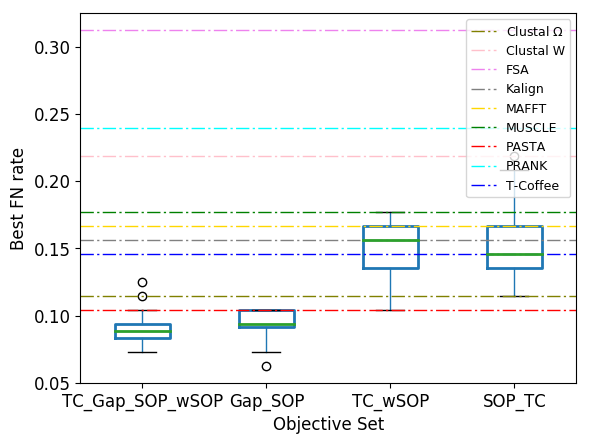
\includegraphics[width=\columnwidth]{Figure/summary/precomputedInit/R0/objset_fnrate_rank}
\caption{R0}
\end{subfigure}    
\begin{subfigure}{0.22\textwidth}
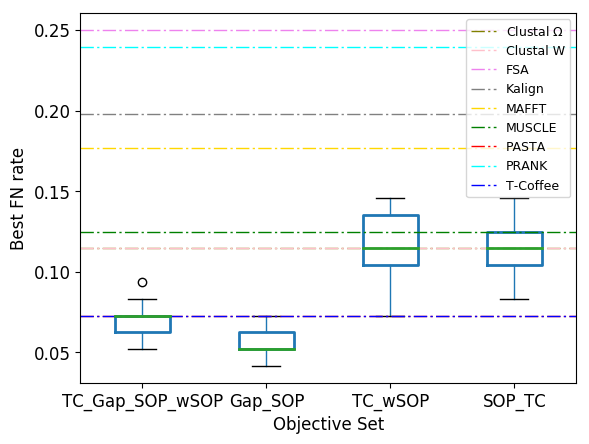
\includegraphics[width=\columnwidth]{Figure/summary/precomputedInit/R4/objset_fnrate_rank}
\caption{R4}
\end{subfigure}
\begin{subfigure}{0.22\textwidth}
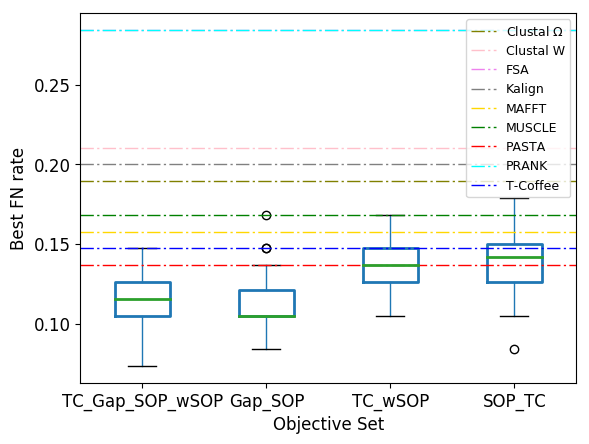
\includegraphics[width=\columnwidth]{Figure/summary/precomputedInit/R9/objset_fnrate_rank}
\caption{R9}
\end{subfigure}
\begin{subfigure}{0.22\textwidth}
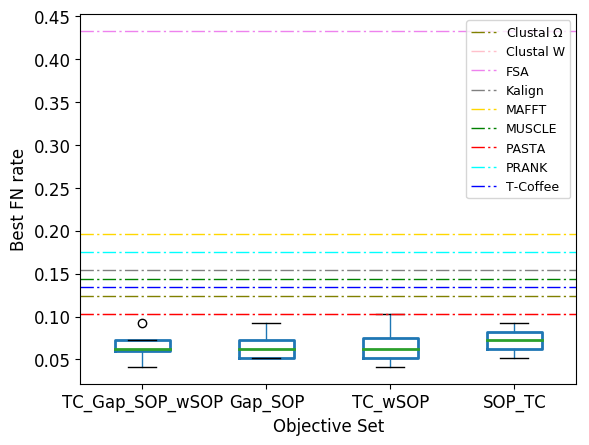
\includegraphics[width=\columnwidth]{Figure/summary/precomputedInit/R14/objset_fnrate_rank}
\caption{R14}
\end{subfigure}
\begin{subfigure}{0.22\textwidth}
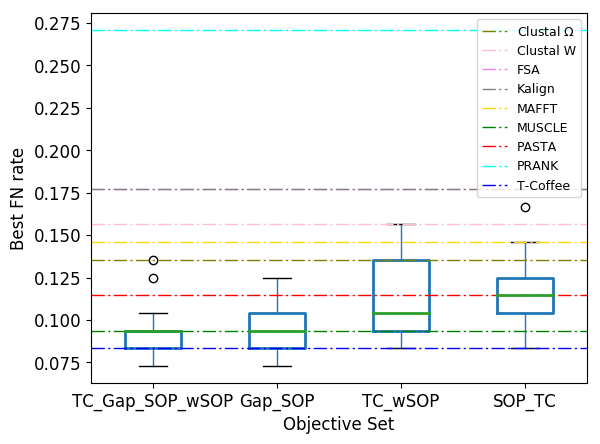
\includegraphics[width=\columnwidth]{Figure/summary/precomputedInit/R19/objset_fnrate_rank}
\caption{R19}
\end{subfigure}
\caption{\underline{100-taxon simulated dataset:} Comparison among objective sets based on the distribution of the collection of the best FN rates from each run. The performance of the state-of-the-art tools are shown using horizontal lines.}
\label{fig:rank_best_fn_rate}
\end{adjustwidth}
\end{figure*}
\end{comment}

\subsubsection{Selecting from three chosen formulations from the literature}
\label{sec:existing_msa_formulation}
To reduce computational burden we carefully study the MO formulations from the literature and pre-select three from among those to focus our research thereon. So we select one from among the three formulations from Table~\ref{tab:abbr} of Section~\ref{sec:methods}. 
Five replicates, namely, R0, R4, R9, R14 and R19, are selected randomly for this experimentation. 



To conduct multivariate linear regression analysis, we need a large pool of diverse alignments. So we run NSGA-III~\citep{deb2014evolutionary} to optimize all objectives (i.e., \{Gap, SOP, wSOP, TC\}) independently for 25 times and combine unique solutions output by each run. Figure~\ref{fig:nature_obj} in the supplementary file presents a $ 4\times4 $ scatter-plot matrix showing the pairwise relationship among all the objectives from this collection. Here we derive the following two important observations.
\begin{enumerate}
	
	\item SOP is entirely correlated with wSOP across all replicates. So optimizing both of them is redundant. Moreover, this high level of correlation causes multicollinearity, a serious trouble in regression analysis~\citep{montgomery2012introduction}. Hence, in the regression model, we will not consider this pair of objectives simultaneously.  
	
	\item Clearly SOP is conflicting with Gap in all cases. So by optimizing them together, many diverse solutions can be generated due to a compromise between these two objectives~\citep{kalyanmoy2001multi}. Such a diverse collection is expected to contain desirable alignment across a variety of datasets.
	
\end{enumerate}

We see inter-dependency among the objective values. Therefore, to avoid getting any spurious result, we want to estimate the correlation between a particular objective function and FN rate keeping the rest of the objectives constant~\citep{montgomery2012introduction}. We accomplish this with the help of the regression model as follows:
\begin{equation}
\small
\begin{split}
\text{FN rate} = \beta_0 + \beta_1 \times \text{TC}+ \beta_2 \times \text{Gap} + 
\beta_3 \times \text{SOP (or wSOP)} + \epsilon \label{eq:multi_lin_reg}
\end{split}
\end{equation}
Here $\epsilon$ is a Gaussian error component with zero mean and some fixed standard deviation. And each coefficient except $\beta_0$ (i.e., the intercept) shows the expected variation in the False Negative rate (i.e., FN rate) per unit variation in the respective objective, rest of the objectives remaining constant. That is why, $\beta_1, \beta_2$ and $\beta_3$ are termed as partial regression coefficients.  
We learn the values of these coefficients (i.e., slopes) using the least-squares method (illustrated using Figure~\ref{fig:mul_lin_reg} in the supplementary file) based on the data (i.e, objective values and FN rates) obtained from the alignments produced by the optimizing of \{Gap, SOP, wSOP, TC\} by NSGA-III. Also, we test the significance of association by applying $t$-test on individual coefficient  $\beta_i$ (with null hypothesis $\beta_i=0$). These regression results allow us to derive two interesting points as follows.
\begin{enumerate}
	\item Gap, SOP and wSOP exhibit better correlation with FN rate (having p-value $<$ 0.05 indicating 95\% confidence) compared to other objective functions in most of the replicates (R0, R4 and R14). So, they are expected to lead towards alignments that can yield better phylogenetic trees.
	\item No objective shows any considerable association in case of R4 and R19 which indicates that an objective might not perform equally across different datasets. 
\end{enumerate}
Next we would like to assess the performance of these MO formulations in terms of FN rate. So for each bi-objective formulation, we independently run NSGA-II~\citep{deb2002fast} 20 times and infer phylogenetic trees for all generated alignments. We have presented the variation of best FN rates collected from each run in a figure in the supplementary file (Figure~\ref{fig:rank_best_fn_rate}). In what follows, We discuss some key observations:
\begin{enumerate}
	\item Naturally giving more objectives to an MO metaheuristics increase its probability of finding the best solution. So we see that the unified formulation \{TC, Gap, SOP, wSOP\} often shows superior performance over the bi-objective formulations. However, in this chapter, we have preferred smaller MO formulations to reduce the overall complexity.
\item \{Gap, SOP\} achieves better FN rates compared to other bi-objective formulations. And its performance is very close to \{TC, Gap, SOP, wSOP\}. This finding conforms the outcome of our regression analysis pointed before.
	\item Both \{Gap, SOP\} and \{TC, Gap, SOP, wSOP\} can consistently outperform the state of the art tools in terms of FN rate.
\end{enumerate}
Based on our experimental results presented above, we can rate \{Gap, SOP\} as the most appropriate among our pre-selected formulations from literature. 


\subsubsection{Selecting a new formulation}
\label{sec:new_msa_formulation}
From the results discussed so far, one may assume that an objective is more desirable if it exhibits a better correlation with the corresponding FN rate.  
So, we try to form a new objective set as follows. As detailed in Section~\ref{sec:formulation}), firstly, we propose four new objective functions, namely, Entropy, SimG, SimNG and GapCon, each of which, quantifies one particular aspect of MSA. We now run NSGA-III in order to optimize the combined objective set, \{Entropy, TC, Gap, SimG, SimNG, GapCon\} (i.e., we include TC and Gap as well), for 40 times thereby generating numerous diverse alignments.
We then employ multivariate linear regression to analyze and assess the correlations between our proposed objective functions and corresponding FN rates (please check Figure~\ref{fig:new_nature_obj} in the supplementary file for a visualization). In what follows we present our key observations in this regard.
\begin{itemize}
	\item Entropy is strongly correlated with SimG which poses an issue in our multiple regression analysis. Therefore, these two objectives should not remain together in our in our regression model; nor should they be combined in the MO formulation.
	
	\item We witness a conflicting relationship between SimG and SimNG. Therefore, through a simultaneous optimization of these two objectives, a MO metaheuristic can expect to generate a (large) number of alignments that are diverse.
\end{itemize}

Now we use the following model to express as well as capture the relationship between the proposed objective functions and the corresponding FN rates:
\begin{equation}
\small
\begin{split}
\text{FN rate} = \beta_0 + \beta_1 \times \text{SimNG}+ \beta_2 \times \text{GapCon} + 
\beta_3 \times \text{SimG (or Entropy)} + \epsilon \label{eq:new_multi_lin_reg}
\end{split}
\end{equation}
Now, the regression coefficients are estimated by fitting the model of Equation \ref{eq:new_multi_lin_reg} to the data (i.e., objective values and FN rates) obtained from a diverse collection of alignments generated by optimizing \{Entropy, TC, Gap, SimG, SimNG, GapCon\}, i.e., the combined objective set. In the sequel, we notice that, both SimG and SimNG exhibit a positive correlation with FN rate. Hence, the objective set \{SimG, SimNG\} is chosen. In the supplementary file, we have presented a visualization using partial regression plots (Figure~\ref{fig:new_mul_lin_reg}).


\subsubsection{Selection mechanism}%{Selection of appropriate multi-objective formulations}
\textit{(The following should be read in conjunction with the description presented in Section~\ref{sec:selection_msa_formulation} of the main text)} 

We visualize the interrelations among the objective values of the solutions, obtained by running NSGA-III to optimizes the objective set \{Gap, SOP, wSOP, TC\} on five randomly selected replicates (R0, R4, R9, R14, R19) of 100-taxon simulated dataset, using a $ 4\times4 $ scatter-plot matrix~\cite{kalyanmoy2001multi} as shown in Figure~\ref{fig:nature_obj}. Here each diagonal cell of a matrix depicts the distribution of the values of an objective function estimated using kernel density estimation which is a non-parametric way to estimate the probability density function of a random variable. And the non-diagonal cells show the correlation between each pair of objective functions. As our evolutionary algorithms tries to minimize all objective functions, we treat the maximization objective values by multiplying with -1. In the sequel, we normalize all the objective values using min-max technique and as such the maximization objectives are turned into minimization ones.

We estimate the coefficients of multiple linear regression model associating FN rate with each of the objective function from \{Gap, SOP, wSOP, TC\} using least-squares method and illustrate them using partial regression plots~\citep{montgomery2012introduction} in Figure~\ref{fig:mul_lin_reg}. We apply $t$-test on individual regression coefficient (i.e., slope) $\beta_i$ (with null hypothesis $\beta_i=0$) to test the significance of that association. The test results (slope, $p$-value) are incorporated in the figure.

We measure the strength of each objective set based on the FN rate achieved by the members of generated solution set. To accomplish this, For each set of objective functions, we run NSGA-II~\citep{deb2002fast} for 20 times following the standard practice of operations research (OR) literature (due to the stochastic nature of metaheuristics). Each run generates a set of solutions that represents the trade-offs in satisfying all objectives. Afterwards, we inferred ML tree for each of the generated alignment. We collected the best FN rates from each of the 20 solution sets and describe the distribution of these FN rates using boxplots which are shown in Figure~\ref{fig:rank_best_fn_rate}. In these boxplots we also incorporate the FN rates achieved by the state-of-the-art tools for comparison using horizontal lines.

\begin{figure*}[!htbp]	
	\begin{adjustwidth}{-1cm}{-1cm}
		\centering
		\begin{subfigure}{0.35\textwidth}
			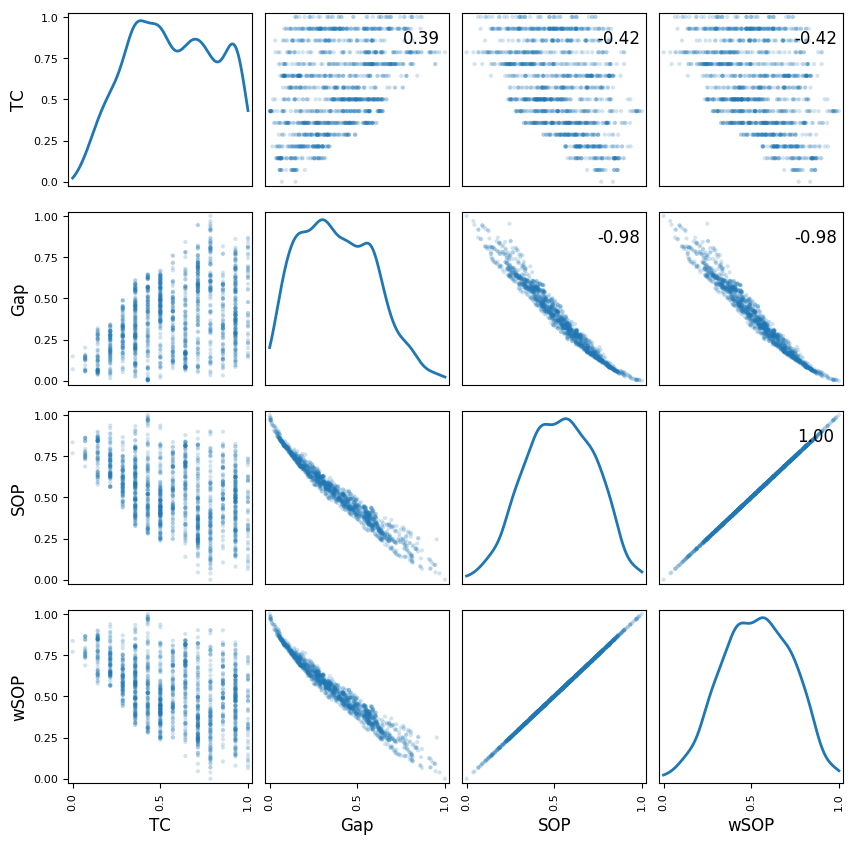
\includegraphics[width=\columnwidth]{Figure/NumGaps_SOP_TC_wSOP/precomputedInit/R0/fig/scatter_mattrix}
			\caption{R0}
			%\label{fig:con_pr09}
		\end{subfigure}	
		\begin{subfigure}{0.35\textwidth}
			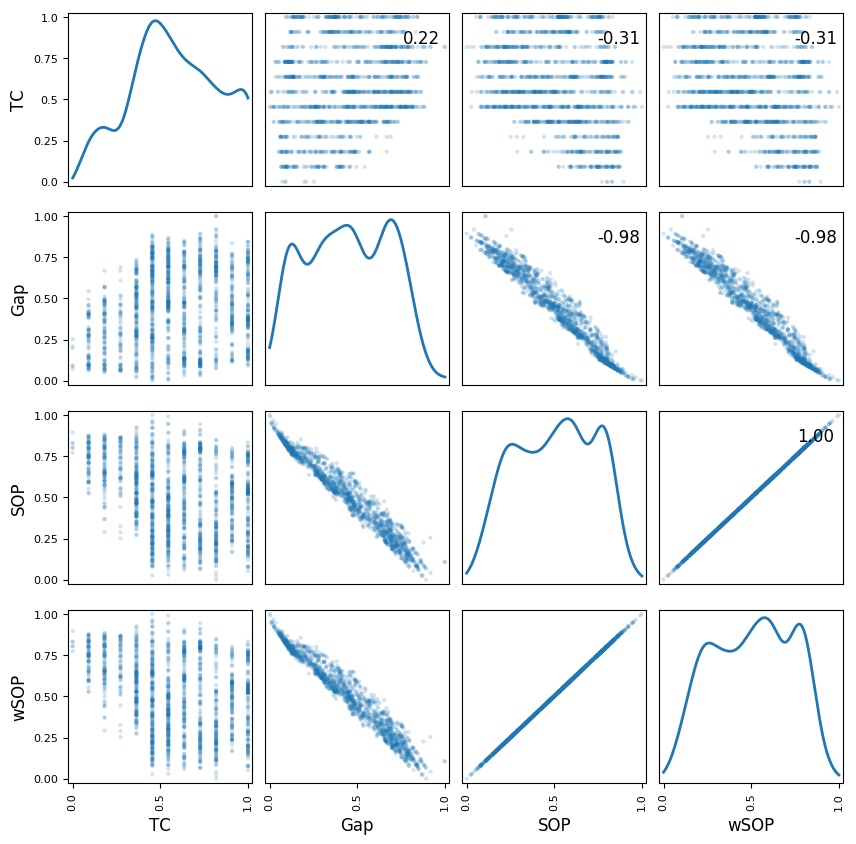
\includegraphics[width=\columnwidth]{Figure/NumGaps_SOP_TC_wSOP/precomputedInit/R4/fig/scatter_mattrix}
			\caption{R4}
			%\label{fig:con_pr09}
		\end{subfigure}
		\begin{subfigure}{0.35\textwidth}
			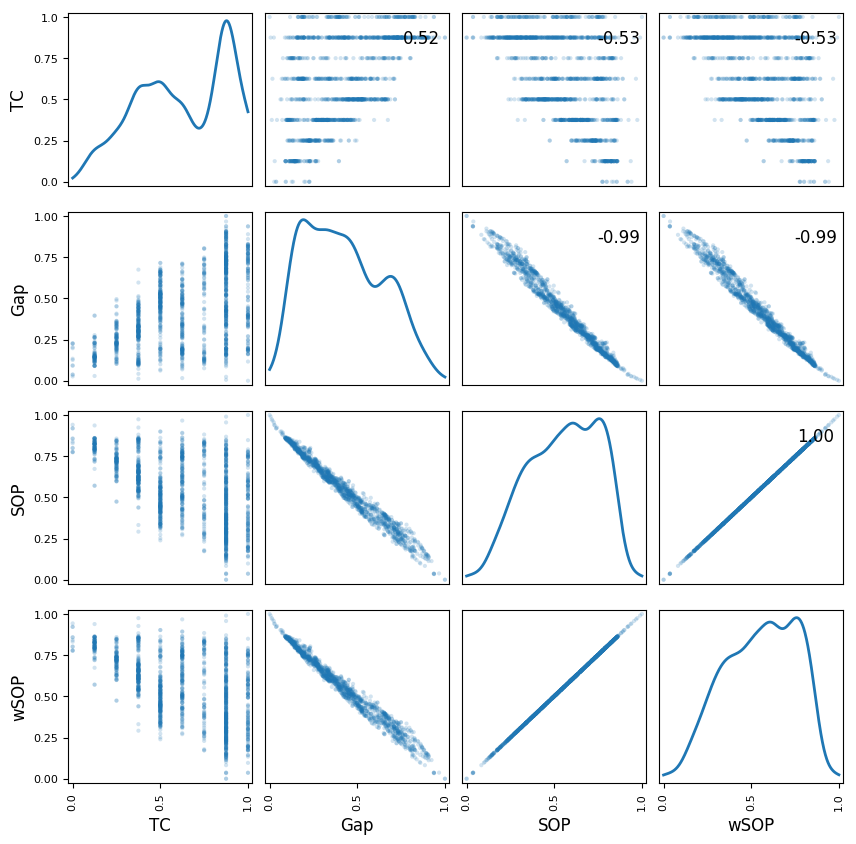
\includegraphics[width=\columnwidth]{Figure/NumGaps_SOP_TC_wSOP/precomputedInit/R9/fig/scatter_mattrix}
			\caption{R9}
			%\label{fig:con_pr09}
		\end{subfigure}
		\begin{subfigure}{0.35\textwidth}
			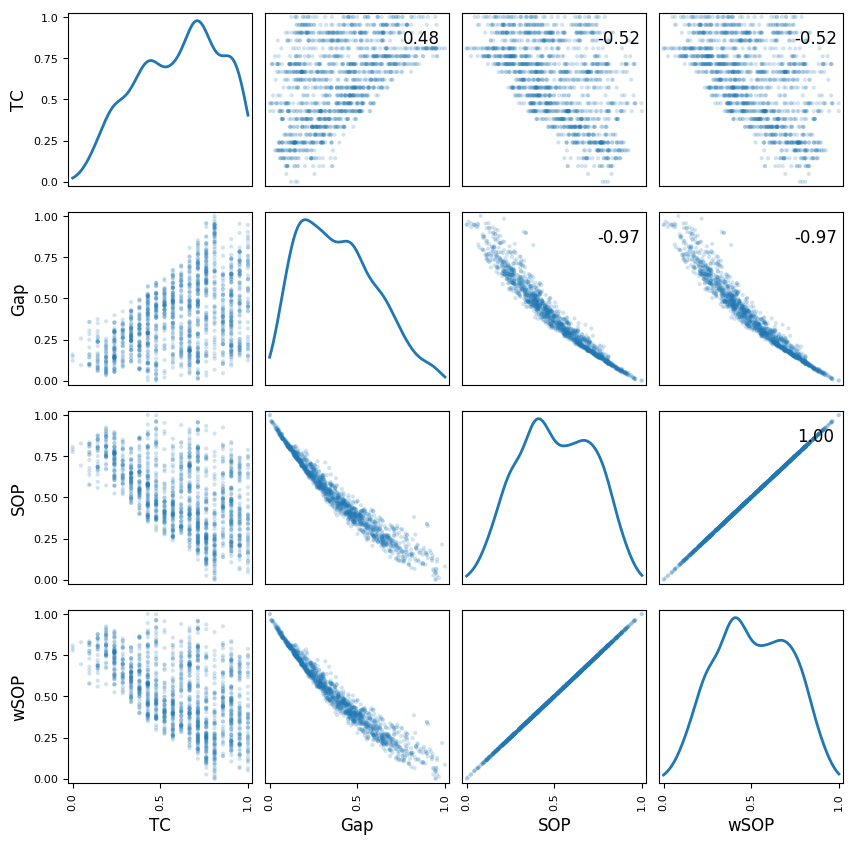
\includegraphics[width=\columnwidth]{Figure/NumGaps_SOP_TC_wSOP/precomputedInit/R14/fig/scatter_mattrix}
			\caption{R14}
			%\label{fig:con_pr09}
		\end{subfigure}
		\begin{subfigure}{0.35\textwidth}
			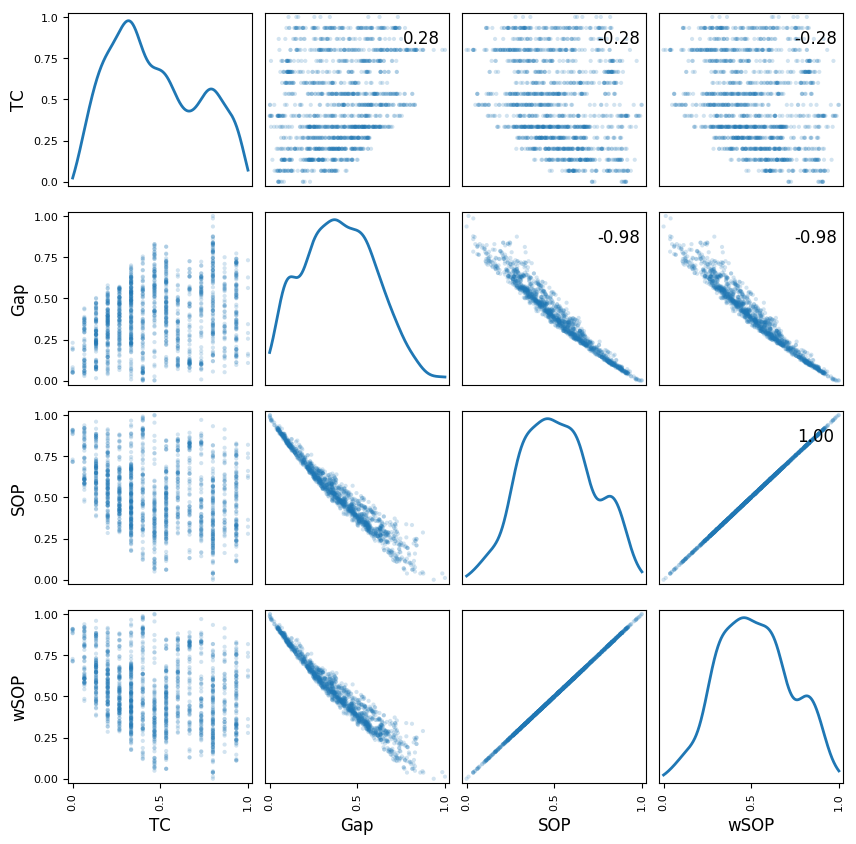
\includegraphics[width=\columnwidth]{Figure/NumGaps_SOP_TC_wSOP/precomputedInit/R19/fig/scatter_mattrix}
			\caption{R19}
			%\label{fig:con_pr09}
		\end{subfigure}
		\caption[Scatter-plot matrices for four objective functions on 100-taxon simulated dataset]{\underline{100-taxon simulated dataset:} Scatter-plot matrices depicting the pairwise relationship of all objective functions on five randomly selected replicates. We turn each objective function into minimization form and then normalize using min-max technique. In each matrix, the diagonal cells show the distribution of objective values (estimated using kernel density estimation which is a non-parametric way to estimate the probability density function of a random variable) while the non-diagonal cells show the correlation between pairs of objective functions. Each upper-diagonal cell contains the value of correlation coefficient $r$ of the corresponding pair of objective functions.}
		\label{fig:nature_obj}
	\end{adjustwidth}
\end{figure*}

\begin{figure*}[!htbp]
	\centering
	\small
	\begin{adjustwidth}{-1cm}{-1cm}
		\begin{tabular}{l||C{0.24\textwidth}|C{0.24\textwidth}|C{0.24\textwidth}|C{0.24\textwidth} }
			& TC & Gap & SOP & wSOP\\\hline\hline
			\rotatebox[origin=c]{-90}{R0} & 
			\raisebox{-.5\height}{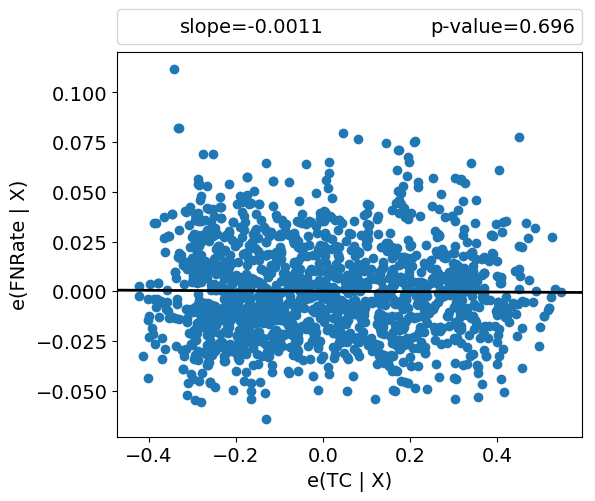
\includegraphics[width=0.22\textwidth]{Figure/NumGaps_SOP_TC_wSOP/precomputedInit/R0/fig/tc_partial_regression}} &
			\raisebox{-.5\height}{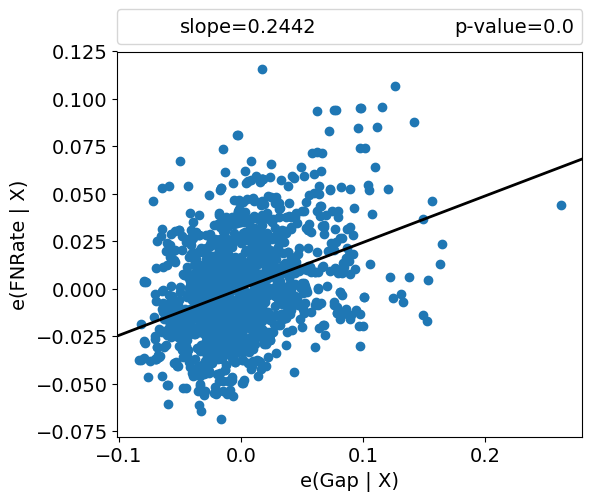
\includegraphics[width=0.22\textwidth]{Figure/NumGaps_SOP_TC_wSOP/precomputedInit/R0/fig/gap_partial_regression}} & 
			\raisebox{-.5\height}{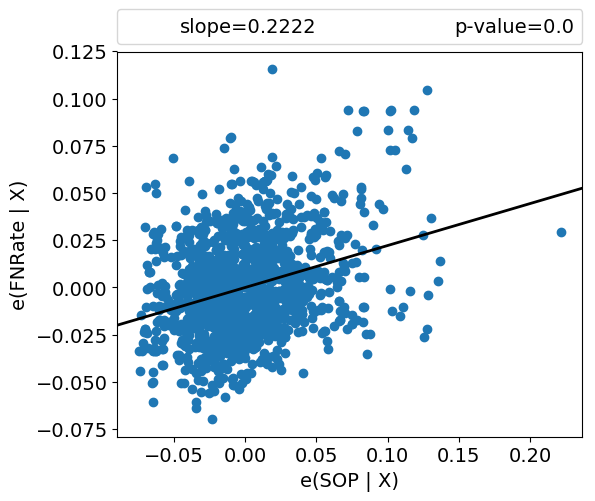
\includegraphics[width=0.22\textwidth]{Figure/NumGaps_SOP_TC_wSOP/precomputedInit/R0/fig/sop_partial_regression}} & 
			\raisebox{-.5\height}{\includegraphics[width=0.22\textwidth]{Figure/NumGaps_SOP_TC_wSOP/precomputedInit/R0/fig/wsop_partial_regression}} 	
			\\\hline
			\rotatebox[origin=c]{-90}{R4} &
			\raisebox{-.5\height}{\includegraphics[width=0.22\textwidth]{Figure/NumGaps_SOP_TC_wSOP/precomputedInit/R4/fig/tc_partial_regression}} &
			\raisebox{-.5\height}{\includegraphics[width=0.22\textwidth]{Figure/NumGaps_SOP_TC_wSOP/precomputedInit/R4/fig/gap_partial_regression}} & 
			\raisebox{-.5\height}{\includegraphics[width=0.22\textwidth]{Figure/NumGaps_SOP_TC_wSOP/precomputedInit/R4/fig/sop_partial_regression}} & 
			\raisebox{-.5\height}{\includegraphics[width=0.22\textwidth]{Figure/NumGaps_SOP_TC_wSOP/precomputedInit/R4/fig/wsop_partial_regression}}
			\\\hline
			\rotatebox[origin=c]{-90}{R9} &
			\raisebox{-.5\height}{\includegraphics[width=0.22\textwidth]{Figure/NumGaps_SOP_TC_wSOP/precomputedInit/R9/fig/tc_partial_regression}} &
			\raisebox{-.5\height}{\includegraphics[width=0.22\textwidth]{Figure/NumGaps_SOP_TC_wSOP/precomputedInit/R9/fig/gap_partial_regression}} & 
			\raisebox{-.5\height}{\includegraphics[width=0.22\textwidth]{Figure/NumGaps_SOP_TC_wSOP/precomputedInit/R9/fig/sop_partial_regression}} & 
			\raisebox{-.5\height}{\includegraphics[width=0.22\textwidth]{Figure/NumGaps_SOP_TC_wSOP/precomputedInit/R9/fig/wsop_partial_regression}}
			\\\hline
			\rotatebox[origin=c]{-90}{R14} &
			\raisebox{-.5\height}{\includegraphics[width=0.22\textwidth]{Figure/NumGaps_SOP_TC_wSOP/precomputedInit/R14/fig/tc_partial_regression}} &
			\raisebox{-.5\height}{\includegraphics[width=0.22\textwidth]{Figure/NumGaps_SOP_TC_wSOP/precomputedInit/R14/fig/gap_partial_regression}} & 
			\raisebox{-.5\height}{\includegraphics[width=0.22\textwidth]{Figure/NumGaps_SOP_TC_wSOP/precomputedInit/R14/fig/sop_partial_regression}} & 
			\raisebox{-.5\height}{\includegraphics[width=0.22\textwidth]{Figure/NumGaps_SOP_TC_wSOP/precomputedInit/R14/fig/wsop_partial_regression}}
			\\\hline
			\rotatebox[origin=c]{-90}{R19} &
			\raisebox{-.5\height}{\includegraphics[width=0.22\textwidth]{Figure/NumGaps_SOP_TC_wSOP/precomputedInit/R19/fig/tc_partial_regression}} &
			\raisebox{-.5\height}{\includegraphics[width=0.22\textwidth]{Figure/NumGaps_SOP_TC_wSOP/precomputedInit/R19/fig/gap_partial_regression}} & 
			\raisebox{-.5\height}{\includegraphics[width=0.22\textwidth]{Figure/NumGaps_SOP_TC_wSOP/precomputedInit/R19/fig/sop_partial_regression}} & 
			\raisebox{-.5\height}{\includegraphics[width=0.22\textwidth]{Figure/NumGaps_SOP_TC_wSOP/precomputedInit/R19/fig/wsop_partial_regression}}
			\\\hline
		\end{tabular}
		\caption[Multiple linear regression model with objective functions from literature for 100-taxon simulated dataset]{\underline{100-taxon simulated dataset:} Multiple linear regression model for identifying the association among FN rate and three objective functions (TC, Gap and SOP/wSOP) fitted to five randomly selected replicates. There is one figure for each possible combination (replicate, objective function). Each partial regression plot shows the association between an objective function and FN rate while holding the remaining two objectives constant. In a plot for an objective function $ OF $, the horizontal axis, $e(OF|X)$, denotes the residuals from regressing $OF$ against the remaining objective functions and the vertical axis, $e(FNRate|X)$, denotes the residuals from regressing FN rate against all the objective functions except $ OF $.} 
		\label{fig:mul_lin_reg}
	\end{adjustwidth}
\end{figure*}

\begin{figure*}[!htbp]
	\centering
	%\begin{adjustwidth}{-1cm}{-1cm}
	\begin{subfigure}{0.32\textwidth}
		\includegraphics[width=\textwidth]{Figure/summary/precomputedInit/R0/objset_fnrate_rank}
		\caption{R0}
		%\label{fig:con_pr09}
	\end{subfigure}	
	\begin{subfigure}{0.32\textwidth}
		\includegraphics[width=\columnwidth]{Figure/summary/precomputedInit/R4/objset_fnrate_rank}
		\caption{R4}
		%\label{fig:con_pr09}
	\end{subfigure}
	\begin{subfigure}{0.32\textwidth}
		\includegraphics[width=\columnwidth]{Figure/summary/precomputedInit/R9/objset_fnrate_rank}
		\caption{R9}
		%\label{fig:con_pr09}
	\end{subfigure}
	
	\begin{subfigure}{0.32\textwidth}
		\includegraphics[width=\columnwidth]{Figure/summary/precomputedInit/R14/objset_fnrate_rank}
		\caption{R14}
		%\label{fig:con_pr09}
	\end{subfigure}
	\begin{subfigure}{0.32\textwidth}
		\includegraphics[width=\columnwidth]{Figure/summary/precomputedInit/R19/objset_fnrate_rank}
		\caption{R19}
		%\label{fig:con_pr09}
	\end{subfigure}
	\caption{\underline{100-taxon simulated dataset:} Comparison among objective sets based on the distribution of the collection of the best FN rates from each run. The performance of the state-of-the-art tools are shown using horizontal lines.}
	\label{fig:rank_best_fn_rate}
	%	\end{adjustwidth}
\end{figure*}


\begin{figure*}[!htbp]	
	\begin{adjustwidth}{-1cm}{-1cm}
		\centering
		\begin{subfigure}{0.35\textwidth}
			\includegraphics[width=\columnwidth]{Figure/6-obj-old/R0/fig/scatter_mattrix}
			\caption{R0}
			%\label{fig:con_pr09}
		\end{subfigure}	
		\begin{subfigure}{0.35\textwidth}
			\includegraphics[width=\columnwidth]{Figure/6-obj-old/R4/fig/scatter_mattrix}
			\caption{R4}
			%\label{fig:con_pr09}
		\end{subfigure}
		\begin{subfigure}{0.35\textwidth}
			\includegraphics[width=\columnwidth]{Figure/6-obj-old/R9/fig/scatter_mattrix}
			\caption{R9}
			%\label{fig:con_pr09}
		\end{subfigure}
		\begin{subfigure}{0.35\textwidth}
			\includegraphics[width=\columnwidth]{Figure/6-obj-old/R14/fig/scatter_mattrix}
			\caption{R14}
			%\label{fig:con_pr09}
		\end{subfigure}
		\begin{subfigure}{0.35\textwidth}
			\includegraphics[width=\columnwidth]{Figure/6-obj-old/R19/fig/scatter_mattrix}
			\caption{R19}
			%\label{fig:con_pr09}
		\end{subfigure}
		\caption[Scatter-plot matrices for six objective functions on 100-taxon simulated dataset]{\underline{100-taxon simulated dataset:} Scatter-plot matrices depicting the pairwise relationship of all objective functions on five randomly selected replicates. We turn each objective function into minimization form and then normalize using min-max technique. In each matrix, the diagonal cells show the distribution of objective values (estimated using kernel density estimation which is a non-parametric way to estimate the probability density function of a random variable) while the non-diagonal cells show the correlation between pairs of objective functions. Each upper-diagonal cell contains the value of correlation coefficient $r$ of the corresponding pair of objective functions.}
		\label{fig:new_nature_obj}
	\end{adjustwidth}
\end{figure*}
\begin{figure*}[!htbp]
	\centering
	\small
	\begin{adjustwidth}{-1cm}{-1cm}
		\begin{tabular}{l||C{0.24\textwidth}|C{0.24\textwidth}|C{0.24\textwidth}|C{0.24\textwidth} }
			& Entropy & GapCon & SimG & SimNG\\\hline\hline
			\rotatebox[origin=c]{-90}{R0} & 
			\raisebox{-.5\height}{\includegraphics[width=0.22\textwidth]{Figure/6-obj-old/precomputedInit/R0/fig/Entropy_partial_regression}} &
			\raisebox{-.5\height}{\includegraphics[width=0.22\textwidth]{Figure/6-obj-old/precomputedInit/R0/fig/GapCon_partial_regression}} & 
			\raisebox{-.5\height}{\includegraphics[width=0.22\textwidth]{Figure/6-obj-old/precomputedInit/R0/fig/SimG_partial_regression}} & 
			\raisebox{-.5\height}{\includegraphics[width=0.22\textwidth]{Figure/6-obj-old/precomputedInit/R0/fig/SimNG_partial_regression}} 	
			\\\hline
			\rotatebox[origin=c]{-90}{R4} &
			\raisebox{-.5\height}{\includegraphics[width=0.22\textwidth]{Figure/6-obj-old/precomputedInit/R4/fig/Entropy_partial_regression}} &
			\raisebox{-.5\height}{\includegraphics[width=0.22\textwidth]{Figure/6-obj-old/precomputedInit/R4/fig/GapCon_partial_regression}} & 
			\raisebox{-.5\height}{\includegraphics[width=0.22\textwidth]{Figure/6-obj-old/precomputedInit/R4/fig/SimG_partial_regression}} & 
			\raisebox{-.5\height}{\includegraphics[width=0.22\textwidth]{Figure/6-obj-old/precomputedInit/R4/fig/SimNG_partial_regression}}
			\\\hline
			\rotatebox[origin=c]{-90}{R9} &
			\raisebox{-.5\height}{\includegraphics[width=0.22\textwidth]{Figure/6-obj-old/precomputedInit/R9/fig/Entropy_partial_regression}} &
			\raisebox{-.5\height}{\includegraphics[width=0.22\textwidth]{Figure/6-obj-old/precomputedInit/R9/fig/GapCon_partial_regression}} & 
			\raisebox{-.5\height}{\includegraphics[width=0.22\textwidth]{Figure/6-obj-old/precomputedInit/R9/fig/SimG_partial_regression}} & 
			\raisebox{-.5\height}{\includegraphics[width=0.22\textwidth]{Figure/6-obj-old/precomputedInit/R9/fig/SimNG_partial_regression}}
			\\\hline
			\rotatebox[origin=c]{-90}{R14} &
			\raisebox{-.5\height}{\includegraphics[width=0.22\textwidth]{Figure/6-obj-old/precomputedInit/R14/fig/Entropy_partial_regression}} &
			\raisebox{-.5\height}{\includegraphics[width=0.22\textwidth]{Figure/6-obj-old/precomputedInit/R14/fig/GapCon_partial_regression}} & 
			\raisebox{-.5\height}{\includegraphics[width=0.22\textwidth]{Figure/6-obj-old/precomputedInit/R14/fig/SimG_partial_regression}} & 
			\raisebox{-.5\height}{\includegraphics[width=0.22\textwidth]{Figure/6-obj-old/precomputedInit/R14/fig/SimNG_partial_regression}}
			\\\hline
			\rotatebox[origin=c]{-90}{R19} &
			\raisebox{-.5\height}{\includegraphics[width=0.22\textwidth]{Figure/6-obj-old/precomputedInit/R19/fig/Entropy_partial_regression}} &
			\raisebox{-.5\height}{\includegraphics[width=0.22\textwidth]{Figure/6-obj-old/precomputedInit/R19/fig/GapCon_partial_regression}} & 
			\raisebox{-.5\height}{\includegraphics[width=0.22\textwidth]{Figure/6-obj-old/precomputedInit/R19/fig/SimG_partial_regression}} & 
			\raisebox{-.5\height}{\includegraphics[width=0.22\textwidth]{Figure/6-obj-old/precomputedInit/R19/fig/SimNG_partial_regression}}
			\\\hline
		\end{tabular}	
		\caption[Multiple linear regression model with our prorposed objective functions for 100-taxon simulated dataset]{\underline{100-taxon simulated dataset:} Multiple linear regression model for identifying the association among FN rate and three objective functions (SimNG, GapCon and SimG/Entropy) fitted to five randomly selected replicates. There is one figure for each possible combination (replicate, objective function). Each partial regression plot shows the association between an objective function and FN rate while holding the remaining two objectives constant.  In a plot for an objective function $ OF $, the horizontal axis, $e(OF|X)$, denotes the residuals from regressing $OF$ against the remaining objective functions and the vertical axis, $e(FNRate|X)$, denotes the residuals from regressing FN rate against all the objective functions except $ OF $.}
		\label{fig:new_mul_lin_reg}
	\end{adjustwidth}
\end{figure*}

\subsection{Evaluation of selected MO formulations}\label{sec:eval_formulation}Now we examine the efficacy of our chosen formulations (i.e., \{SimG, SimNG\} and \{Gap, SOP\}) based on two biological rRNA datasets and 27 BAliBASE instances. To accomplish this we conduct several repeated runs of NSGA-II on these datasets. Then we examine the generated alignments based on the alignment quality as well as based on the resultant phylogenetic trees.

\subsubsection{Results achieved on biological rRNA datasets}
\begin{figure*}[!htbp]
	\centering
	\begin{adjustwidth}{-0.5cm}{-0.5cm}
		\begin{subfigure}[b]{0.25\textwidth}
			\includegraphics[width=\columnwidth]{Figure/summary/precomputedInit/23S.E/fnrate_density_single_run}
			\caption{23S.E}
\end{subfigure}    
		\begin{subfigure}[b]{0.25\textwidth}
			\includegraphics[width=\columnwidth]{Figure/summary/precomputedInit/23S.E.aa_ag/fnrate_density_single_run}
			\caption{23S.E.aa\_ag}
\end{subfigure}
		\begin{subfigure}[b]{0.25\textwidth}
			\includegraphics[width=\columnwidth]{Figure/summary/precomputedInit/23S.E/objset_fnrate_rank}
			\caption{23S.E}
\end{subfigure}    
		\begin{subfigure}[b]{0.25\textwidth}
			\includegraphics[width=\columnwidth]{Figure/summary/precomputedInit/23S.E.aa_ag/objset_fnrate_rank}
			\caption{23S.E.aa\_ag}
\end{subfigure}
\begin{subfigure}{0.25\textwidth}
			\includegraphics[width=\columnwidth]{Figure/summary/precomputedInit/23S.E/tc_density_single_run}
			\caption{23S.E}
\end{subfigure}    
		\begin{subfigure}{0.25\textwidth}
			\includegraphics[width=\columnwidth]{Figure/summary/precomputedInit/23S.E.aa_ag/tc_density_single_run}
			\caption{23S.E.aa\_ag}
\end{subfigure}
		\begin{subfigure}{0.25\textwidth}
			\includegraphics[width=\columnwidth]{Figure/summary/precomputedInit/23S.E/objset_tc_rank}
			\caption{23S.E}
\end{subfigure}    
		\begin{subfigure}{0.25\textwidth}
			\includegraphics[width=\columnwidth]{Figure/summary/precomputedInit/23S.E.aa_ag/objset_tc_rank}
			\caption{23S.E.aa\_ag}
\end{subfigure}
\begin{subfigure}{0.25\textwidth}
			\includegraphics[width=\columnwidth]{Figure/summary/precomputedInit/23S.E/pairs_density_single_run}
			\caption{23S.E}
\end{subfigure}    
		\begin{subfigure}{0.25\textwidth}
			\includegraphics[width=\columnwidth]{Figure/summary/precomputedInit/23S.E.aa_ag/pairs_density_single_run}
			\caption{23S.E.aa\_ag}
\end{subfigure}
		\begin{subfigure}{0.25\textwidth}
			\includegraphics[width=\columnwidth]{Figure/summary/precomputedInit/23S.E/objset_pairs_rank}
			\caption{23S.E}
\end{subfigure}    
		\begin{subfigure}{0.25\textwidth}
			\includegraphics[width=\columnwidth]{Figure/summary/precomputedInit/23S.E.aa_ag/objset_pairs_rank}
			\caption{23S.E.aa\_ag}
\end{subfigure}
\begin{subfigure}{0.26\textwidth}
			\includegraphics[width=\columnwidth]{Figure/summary/precomputedInit/23S.E/fnrate_vs_tc}
			\caption{23S.E}
\end{subfigure}    
		\begin{subfigure}{0.26\textwidth}
			\includegraphics[width=\columnwidth]{Figure/summary/precomputedInit/23S.E.aa_ag/fnrate_vs_tc}
			\caption{23S.E.aa\_ag}
\end{subfigure}
		\begin{subfigure}{0.26\textwidth}
			\includegraphics[width=\columnwidth]{Figure/summary/precomputedInit/23S.E/fnrate_vs_sp}
			\caption{23S.E}
\end{subfigure}    
		\begin{subfigure}{0.26\textwidth}
			\includegraphics[width=\columnwidth]{Figure/summary/precomputedInit/23S.E.aa_ag/fnrate_vs_sp}
			\caption{23S.E.aa\_ag}
\end{subfigure}
	
	\caption[Results on biological rRNA datasets]{\underline{Results on biological rRNA datasets:} \textbf{Panel 1 (Top Panel):} part (a) and part (b) show the FN rates yielded from 100 final population members averaged across 10 independent executions of NSGA-II. Before averaging, we sort the 100 FN rates obtained per run. Next we calculate the average of the best FN rates acquired from 10 executions. We repeat this for the second best FN rates and so on.
		part (c) and part (d) show the variation of the best FN rates obtained across 10 runs using boxplots.  \textbf{Panel 2 (Panel 3):} part (e) and part (f) (part (i) and part (j)) show the 100 TC scores (SP scores) averaged across 10 executions. 
part (g) and part (h) (part (k) and part (l)) show the variations of the best TC (SP) scores collected from 10 executions.
\textbf{Panel 4 (Bottom panel):} part (m) and part (n) show the relationship between TC score and FN rate for various alignments. part (o) and part (p) show the relationship between SP score and FN rate. In each panel, the score achieved by nine MSA methods are shown using horizontal dashed lines.
	}
	\label{fig:fn_rate_tc_sp_bio}
\end{adjustwidth}
\end{figure*}
We have run NSGA-II (10 independent runs) optimizing our two selected objective sets on two datasets (23S.E \& 23S.E.aa\_ag). 
We report the performance comparison of the MO formulations against the nine state of the art tools in terms of FN rate in Figure~\ref{fig:fn_rate_tc_sp_bio} (top panel). Here, part (a) and part (b) show the FN rate obtained from 100 alignments (i.e., members of the final population) averaged across 10 runs. To get these averaged FN rates, we sort the FN rates 100 solutions generated per run in ascending order. Next we calculate the average of the lowest FN rates acquired from all of these runs. We repeat this for the second lowest ones and so on. These figures (part (a) and (b)) demonstrate a promising aspect of MO approach that for each data it can generate a substantial number of solutions that are superior than the outputs of state-of-the-art tools. However, a practitioner would be interested in the best solutions. Therefore, we summarize the best FN rate over 10 runs in part (c) and (d). For both datasets, we see that, among the nine tools, FSA performed the best, followed by PRANK in 23.S.E dataset and PASTA in 23S.E.aa\_ag dataset. The two MO formulations yielded improved FN rates compared to FSA in 23S.E.aa\_ag dataset (part (b) and part (d)). In fact, on average, the optimization of \{Gap, SOP\} produces around 10\% (40\%) solutions that are superior to FSA (PASTA) as illustrated in part (b). On the contrary, the set \{SimG, SimNG\}, while produces around 40\% solutions that are better than PASTA on average, is able to produce very few solutions that are better than FSA. As can be noticed from Part (d), \{Gap, SOP\} is able to consistently outperform the best tool (i.e., FSA) and in almost 40\% of the total runs, \{SimG, SimNG\} also outperforms FSA . Now we focus on the results for 23S.E dataset (part (a) and (c)).  In this case, both \{Gap, SOP\} and \{SimG, SimNG\} remain below the best (FSA) but above the second best (PRANK) tool by generating around 5\% solutions better than the latter.


We similarly analyze SP and TC scores and illustrate the results in Figure~\ref{fig:fn_rate_tc_sp_bio}. Evidently, the alignments generated by MO formulations, according to the two popular above-mentioned measures, could not outperform the best performing tool, PASTA.
Panel 4 of Figure~\ref{fig:fn_rate_tc_sp_bio} clearly illustrates the discrepancy between TC (SP) score and FN rate; please check part (m) and part (n) (part (o) and part (p)).
To summarize, the MSA methods exhibiting superiority than our MO formulations with respect to the widely accepted measures cannot attain better phylogenetic trees than our MO formulations (Panel 4 of Figure~\ref{fig:fn_rate_tc_sp_bio}). To elaborate, our objective sets have generated several alignments with lower (i.e., worse) TC scores than PASTA, which is the best performer among the nine state of the art tools according to TC score.  
Contrastingly however, these alignments have produced better phylogenetic trees (i.e., trees having better FN rates) than those tools. Moreover we witness discordance between FN rate and TC score from among the tools: while PASTA is the best performer in terms of the latter, it is in fact behind FSA in terms of the former. Similarly, a quick check of the comparison between SP score and FN rate illustrated in part (o) and part (p) of Panel 4 reveals that there are several alignments generated by the MO formulations with worse SP score than PASTA; however, trees produced by these alignments achieve better FN rates than that tool.   

\begin{table}[!h]
\centering
	\caption{Comparison of 100 solutions generated by one execution of NSGA-II with exis MSA ting nine MSA methods in terms of FN rate.} \includegraphics[width=0.8\columnwidth]{Figure/comparison_gap_sop}
	\label{tab:balibase_good_solutions}
\end{table}




\begin{figure*}[!htbp]
	\begin{adjustwidth}{-1cm}{-1cm}
		\centering
		\begin{subfigure}[b]{0.26\textwidth}
			\includegraphics[width=\columnwidth]{Figure/summary/precomputedInit/Balibase/BB11005_fnrate_density_single_run}
			\caption{BB11005}
\end{subfigure}    
		\begin{subfigure}[b]{0.26\textwidth}
			\includegraphics[width=\columnwidth]{Figure/summary/precomputedInit/Balibase/BB11018_fnrate_density_single_run}
			\caption{BB11018}
\end{subfigure}
		\begin{subfigure}[b]{0.26\textwidth}
			\includegraphics[width=\columnwidth]{Figure/summary/precomputedInit/Balibase/BB11020_fnrate_density_single_run}
			\caption{BB11020}
\end{subfigure}
		\begin{subfigure}[b]{0.26\textwidth}
			\includegraphics[width=\columnwidth]{Figure/summary/precomputedInit/Balibase/BB11033_fnrate_density_single_run}
			\caption{BB11033}
\end{subfigure}
\begin{subfigure}{0.26\textwidth}
			\includegraphics[width=\columnwidth]{Figure/summary/precomputedInit/Balibase/BB11005_objset_fnrate_rank}
			\caption{BB11005}
\end{subfigure}    
		\begin{subfigure}{0.26\textwidth}
			\includegraphics[width=\columnwidth]{Figure/summary/precomputedInit/Balibase/BB11018_objset_fnrate_rank}
			\caption{BB11018}
\end{subfigure}
		\begin{subfigure}{0.26\textwidth}
			\includegraphics[width=\columnwidth]{Figure/summary/precomputedInit/Balibase/BB11020_objset_fnrate_rank}
			\caption{BB11020}
\end{subfigure}
\begin{subfigure}{0.26\textwidth}
			\includegraphics[width=\columnwidth]{Figure/summary/precomputedInit/Balibase/BB11033_objset_fnrate_rank}
			\caption{BB11033}
\end{subfigure}
		
\begin{subfigure}{0.26\textwidth}
			\includegraphics[width=\columnwidth]{Figure/summary/precomputedInit/Balibase/BB11005_fnrate_vs_tc_2}
			\caption{BB11005}
\end{subfigure}    
		\begin{subfigure}{0.26\textwidth}
			\includegraphics[width=\columnwidth]{Figure/summary/precomputedInit/Balibase/BB11018_fnrate_vs_tc_2}
			\caption{BB11018}
\end{subfigure}
		\begin{subfigure}{0.26\textwidth}
			\includegraphics[width=\columnwidth]{Figure/summary/precomputedInit/Balibase/BB11020_fnrate_vs_tc_2}
			\caption{BB11020}
\end{subfigure}
		\begin{subfigure}{0.26\textwidth}
			\includegraphics[width=\columnwidth]{Figure/summary/precomputedInit/Balibase/BB11033_fnrate_vs_tc_2}
			\caption{BB11033}
\end{subfigure}    
		\begin{subfigure}{0.26\textwidth}
			\includegraphics[width=\columnwidth]{Figure/summary/precomputedInit/Balibase/BB11005_fnrate_vs_sp_2}
			\caption{BB11005}
\end{subfigure}    
		\begin{subfigure}{0.26\textwidth}
			\includegraphics[width=\columnwidth]{Figure/summary/precomputedInit/Balibase/BB11018_fnrate_vs_sp_2}
			\caption{BB11018}
\end{subfigure}
		\begin{subfigure}{0.26\textwidth}
			\includegraphics[width=\columnwidth]{Figure/summary/precomputedInit/Balibase/BB11020_fnrate_vs_sp_2}
			\caption{BB11020}
\end{subfigure}
		\begin{subfigure}{0.26\textwidth}
			\includegraphics[width=\columnwidth]{Figure/summary/precomputedInit/Balibase/BB11033_fnrate_vs_sp_2}
			\caption{BB11033}
\end{subfigure}
	
	\caption[Results on RV11 based on tree quality]{ \underline{Results on RV11 based on tree quality:} \textbf{Panel 1 (Top panel):} part (a) - (d) show the averaged 100 (i.e., population size) FN rates obtained across 20 repeated executions of NSGA-II. 
\textbf{Panel 2:} part (e) - (h) show the variation of best FN rates accumulated from 20 repeated executions using boxplots. 
	\textbf{Panel 3 (Panel 4):} part (i) - (l) (part (m) - (p)) show the relationship between TC score (SP score) and FN rate obtained from various alignments. In each panel, FN rates attained by the existing MSA tools are shown using horizontal dashed lines.}
	\label{fig:rv11_fn_rate_tc_sp}
\end{adjustwidth}
\end{figure*}


\begin{figure*}[!htbp]
	\begin{adjustwidth}{-1cm}{-1cm}
		\centering
		\begin{subfigure}[b]{0.26\textwidth}
			\includegraphics[width=\columnwidth]{Figure/summary/precomputedInit/Balibase/BB11005_tc_density_single_run_2}
			\caption{BB11005}
\end{subfigure}    
		\begin{subfigure}[b]{0.26\textwidth}
			\includegraphics[width=\columnwidth]{Figure/summary/precomputedInit/Balibase/BB11018_tc_density_single_run_2}
			\caption{BB11018}
\end{subfigure}
		\begin{subfigure}[b]{0.26\textwidth}
			\includegraphics[width=\columnwidth]{Figure/summary/precomputedInit/Balibase/BB11020_tc_density_single_run_2}
			\caption{BB11020}
\end{subfigure}
\begin{subfigure}[b]{0.26\textwidth}
			\includegraphics[width=\columnwidth]{Figure/summary/precomputedInit/Balibase/BB11033_tc_density_single_run_2}
			\caption{BB11033}
\end{subfigure}
		\begin{subfigure}{0.26\textwidth}
			\includegraphics[width=\columnwidth]{Figure/summary/precomputedInit/Balibase/BB11005_objset_tc_rank_2}
			\caption{BB11005}
\end{subfigure}    
		\begin{subfigure}{0.26\textwidth}
			\includegraphics[width=\columnwidth]{Figure/summary/precomputedInit/Balibase/BB11018_objset_tc_rank_2}
			\caption{BB11018}
\end{subfigure}
		\begin{subfigure}{0.26\textwidth}
			\includegraphics[width=\columnwidth]{Figure/summary/precomputedInit/Balibase/BB11020_objset_tc_rank_2}
			\caption{BB11020}
\end{subfigure}
\begin{subfigure}{0.26\textwidth}
			\includegraphics[width=\columnwidth]{Figure/summary/precomputedInit/Balibase/BB11033_objset_tc_rank_2}
			\caption{BB11033}
\end{subfigure}
		
\begin{subfigure}{0.26\textwidth}
			\includegraphics[width=\columnwidth]{Figure/summary/precomputedInit/Balibase/BB11005_pairs_density_single_run_2}
			\caption{BB11005}
\end{subfigure}    
		\begin{subfigure}{0.26\textwidth}
			\includegraphics[width=\columnwidth]{Figure/summary/precomputedInit/Balibase/BB11018_pairs_density_single_run_2}
			\caption{BB11018}
\end{subfigure}
		\begin{subfigure}{0.26\textwidth}
			\includegraphics[width=\columnwidth]{Figure/summary/precomputedInit/Balibase/BB11020_pairs_density_single_run_2}
			\caption{BB11020}
\end{subfigure}
\begin{subfigure}{0.26\textwidth}
			\includegraphics[width=\columnwidth]{Figure/summary/precomputedInit/Balibase/BB11033_pairs_density_single_run_2}
			\caption{BB11033}
\end{subfigure}
		\begin{subfigure}{0.26\textwidth}
			\includegraphics[width=\columnwidth]{Figure/summary/precomputedInit/Balibase/BB11005_objset_pairs_rank_2}
			\caption{BB11005}
\end{subfigure}    
		\begin{subfigure}{0.26\textwidth}
			\includegraphics[width=\columnwidth]{Figure/summary/precomputedInit/Balibase/BB11018_objset_pairs_rank_2}
			\caption{BB11018}
\end{subfigure}
		\begin{subfigure}{0.26\textwidth}
			\includegraphics[width=\columnwidth]{Figure/summary/precomputedInit/Balibase/BB11020_objset_pairs_rank_2}
			\caption{BB11020}
\end{subfigure}
\begin{subfigure}{0.26\textwidth}
			\includegraphics[width=\columnwidth]{Figure/summary/precomputedInit/Balibase/BB11033_objset_pairs_rank_2}
			\caption{BB11033}
\end{subfigure}
	\end{adjustwidth}
	\caption[Results on RV11 based on alignment quality]{\underline{Results on RV11 based on alignment quality:} \textbf{Panel 1 (Panel 3)}: part (a) - (d) (part (i) - (l)) shows the averaged 100 TC scores (SP scores) obtained across 20 repeated executions of NSGA-II. 
\textbf{Panel 2 (Panel 4)}: part (e) - (h) (part (m) - (p)) shows the variation of best TC scores (SP scores) accumulated from 20 20 repeated executions using boxplots. In each panel, the score attained by existing MSA tools are shown  using horizontal dashed lines.}
	\label{fig:rv11_tc_sp}
	
\end{figure*}

\begin{figure*}[!h]
	\begin{adjustwidth}{-1cm}{-1cm}
		\centering
		\begin{subfigure}[b]{0.25\textwidth}
			\includegraphics[width=\columnwidth]{Figure/tree/BB20010_true_tree}
			\caption{True tree}
\end{subfigure}    
		\begin{subfigure}[b]{0.25\textwidth}
			\includegraphics[width=\columnwidth]{Figure/tree/BB20010_simg_tree}
			\caption{NSGA-II$_{\text{\{SimG, SimNG\}}}$}
\end{subfigure}
		\begin{subfigure}[b]{0.25\textwidth}
			\includegraphics[width=\columnwidth]{Figure/tree/BB20010_gap_tree}
			\caption{NSGA-II$_{\text{\{Gap, SOP\}}}$}
\end{subfigure}
		\begin{subfigure}[b]{0.25\textwidth}
			\includegraphics[width=\columnwidth]{Figure/tree/BB20010_fsa_tree}
			\caption{FSA}
\end{subfigure}
	\end{adjustwidth}
	\caption{ True phylogenetic tree along with the best estimated trees yielded by the two selected MO formulations and FSA method for BB20010.}
	\label{fig:bb20010_trees}
\end{figure*}
\subsubsection{Results on BAliBASE datasets}
We performed 20 repeated runs of NSGA-II on 27 random instances of BAliBASE 3.0. Once again we analyze obtained solutions in terms of the quality measures of alignments and phylogenetic trees and observe that the better alignments according to popular alignment measures, do not necessarily yield better phylogenetic trees.
Due to space constraints, we present our core observations on four instances (BB11018, BB11005, BB11033 \& BB11020 ) under RV11 group in Figures \ref{fig:rv11_fn_rate_tc_sp} and \ref{fig:rv11_tc_sp}. We obtained similar results for the remaining groups (RV12 to RV50) (please see Section~\ref{sec:result_balibase} in the supplementary file). Figure \ref{fig:rv11_fn_rate_tc_sp}) summarizes our findings based on FN rate. If we check the Top panel (part (a) - (h)), we find that, throughout all the instances, the solutions generated by the two objective sets are either better or at least equivalent when compared to the solutions generated by the best tool.  
For BB11020, the objective set \{SimG, SimNG\} achieves 12\% FN rate as opposed to 50\%, achieved by the best tool- clearly, a huge improvement. In terms of TC score however, the two objective sets have been able to outperform all the tools only for BB11020 (part (a) - part (h) of Figure \ref{fig:rv11_tc_sp}), which is conflicting with our findings in terms of the FN rate. So again we witness the discrepancy between TC score and FN rate illustrated in part (i) - part (l) of Figure~\ref{fig:rv11_fn_rate_tc_sp}. On the other hand, Figure \ref{fig:rv11_tc_sp} depicts the results based on SP and TC scores. If we observe its Panel 1 (part (i) - (p)), we see similar disagreement between SP score and FN rate depicted in part (m) - part (p) of Figure~\ref{fig:rv11_fn_rate_tc_sp}. It is clearly evident from these figures that the best TC and/or SP scores may not necessarily imply the best FN rates. This phenomenon is also observed quite consistently across rest of the instances. This finding may be of vital importance for researchers and practitioners, who leverage MSA methods in phylogenetic applications, 

\begin{table*}[!h]
	\scriptsize
	\centering
	\caption{Friedman test and Holm's post-hoc procedure. \underline{Friedman's rank (Column 2):} Average rank (lower rank indicates better) of the MSA approaches. \underline{Holm's adjusted $p$-values (Columns 3, 4 and 5):} Significance of difference between the metaheuristics and the MSA methods.}
	\begin{tabular}{|l|r||c|c|c|}
		\hline
		\multicolumn{1}{|c|}{1} & \multicolumn{1}{c||}{2} & 3     & 4     & 5 \\
		\hline
		\multicolumn{1}{|c|}{\multirow{2}{*}{Method}} & \multirow{2}{*}{Friedman's Rank*} & \multicolumn{3}{c|}{Holm's adjusted $p$-value} \\
		\cline{3-5}      &  & \multicolumn{1}{l|}{NSGA-II$_{\text{\{SimG, SimNG\}}}$} & \multicolumn{1}{l|}{MOEA/D$_{\text{\{SimG, SimNG\}}}$} & \multicolumn{1}{l|}{NSGA-II$_{\text{\{Gap, SOP\}}}$} \\
		\hline
		NSGA-II$_{\text{\{SimG, SimNG\}}}$ & 2.4630 & -     & \multicolumn{1}{r|}{1.00000} & \multicolumn{1}{r|}{1.00000} \\
		\hline
		MOEA/D$_{\text{\{SimG, SimNG\}}}$ & 3.1852 & \multicolumn{1}{r|}{1.00000} & -     &  \multicolumn{1}{r|}{1.00000} \\
		\hline
		NSGA-II$_{\text{\{Gap, SOP\}}}$ & 3.4444 & \multicolumn{1}{r|}{1.00000} &    \multicolumn{1}{r|}{1.00000}   & - \\
		\hline
		ProbCons & 6.6667 & \multicolumn{1}{r|}{0.00086} & \multicolumn{1}{r|}{0.01593} & \multicolumn{1}{r|}{0.04100} \\
		\hline
		Clustal $\Omega$ & 7.2222 & \multicolumn{1}{r|}{0.00007} & \multicolumn{1}{r|}{0.00171} & \multicolumn{1}{r|}{0.00497} \\
		\hline
		MAFFT & 7.3148 & \multicolumn{1}{r|}{0.00004} & \multicolumn{1}{r|}{0.00118} & \multicolumn{1}{r|}{0.00344} \\
		\hline
		Kalign & 7.5556 & \multicolumn{1}{r|}{0.00001} & \multicolumn{1}{r|}{0.00041} & \multicolumn{1}{r|}{0.00126} \\
		\hline
		PASTA & 7.7222 & \multicolumn{1}{r|}{0.00001} & \multicolumn{1}{r|}{0.00019} & \multicolumn{1}{r|}{0.00063} \\
		\hline
		FSA   & 7.8333 & \multicolumn{1}{r|}{0.00000} & \multicolumn{1}{r|}{0.00012} & \multicolumn{1}{r|}{0.00039} \\
		\hline
		MUSCLE & 8.0370 & \multicolumn{1}{r|}{0.00000} & \multicolumn{1}{r|}{0.00004} & \multicolumn{1}{r|}{0.00015} \\
		\hline
		Clustal W & 8.2037 & \multicolumn{1}{r|}{0.00000} & \multicolumn{1}{r|}{0.00002} & \multicolumn{1}{r|}{0.00007} \\
		\hline
		RetAlign & 8.3519 & \multicolumn{1}{r|}{0.00000} & \multicolumn{1}{r|}{0.00001} & \multicolumn{1}{r|}{0.00003} \\
		\hline
		\hline
		*Statistic & 14.3760 & \multicolumn{3}{c|}{\multirow{2}{*}{N/A}} \\
		\cline{1-2}    *$p$-value & 0.0000 & \multicolumn{3}{c|}{} \\
		\hline
	\end{tabular}\label{tab:friedman_holm}\end{table*}



Table~\ref{tab:balibase_good_solutions} shows a comparison of the averaged 100 FN rates yielded through a single execution of NSGA-II by optimizing the formulation, \{Gap, SOP\} against the existing MSA methods in terms of FN rate for the BAliBASE datasets. It shows that, on most of the cases, the MO approach can yield better phylogenetic trees than all MSA methods. As an illustration, for BB20010 we show the true tree and the most accurate estimated trees yielded by the two selected MO formulations and FSA (performed best among the nine MSA methods) in Figure~\ref{fig:bb20010_trees}. We further conducted a comparative analysis between NSGA-II and MOEA/D while optimizing \{SimG, SimNG\}. However, due to space constraints, the results are reported in Table~\ref{tab:balibase_good_solutions_simg_simng} and ~\ref{tab:superior_solutions} of the supplementary file.




\subsubsection{Statistical tests}
Here we assess whether the observed improvements in terms of FN rate attained by the MO formulations over the nine  MSA tools are statistically significant.
We apply an appropriate statistical significance test on 27 BAliBASE instances. So we gather paired data using the FN rate attained for each of the (MSA method, instance) pairs. In case of our metaheuristics, the average of the best (i.e., lowest) FN rates obtained from 20 repeated executions is taken. Since our data do not comply with the assumption of homoscedasticity and normality, following the suggestion of~\cite{derrac2011practical}, we have applied, with 95\% confidence level, a series of nonparametric tests.  


We first perform a (nonparametric) test due to Friedman (popularly known as the Friedman Test). Thus we are able to rank (lower rank implies better) all the methods as reported in Column 2 of Table~\ref{tab:friedman_holm}. We notice that the MO approaches are clearly ahead of the existing MSA tools. Next, we follow Holm's post-hoc procedure and report the adjusted $p$-value that indicates the significance of the difference in the FN rate between two methods thereby complementing the Friedman test rankings. The adjusted $p$-values are presented Columns 3 to 5 of the same table. 
These values show that the observed difference (i.e., improved FN rates) between a MO approach and each of the nine MSA tools are statistically significant (adjusted $p$-value $\le$ 0.05).

\begin{table}[htbp]
	\centering
	\caption{Overall performance (worst: 0, best: 10) of our proposed methodology across six subgroups of BAliBASE datasets.}
	\begin{tabular}{|c|r|}
		\hline
		Group & \multicolumn{1}{l|}{Avg. Score} \\
		\hline
		RV11  & 4.25 \\
		\hline
		RV12  & 8.4 \\
		\hline
		RV20  & 3.4 \\
		\hline
		RV30  & 5.25 \\
		\hline
		RV40  & 8 \\
		\hline
		RV50  & 6 \\
		\hline
	\end{tabular}%
	\label{tab:insight_group}%
\end{table}%

\subsection{Biological Perspective}\label{sec:discussion}
% Table generated by Excel2LaTeX from sheet 'Sheet1'
Here we attempt to characterize the overall performance of our proposed methodology using a biological perspective. To accomplish this, using the values reported in Table~\ref{tab:superior_solutions}, we systematically score the overall performance (worst: 0, best: 10) of our approach on a particular dataset. Then we categorize 27 biological instances of BAliBASE benchmark into different groups based on following biological criteria further analyze the performance of our approach.
\begin{itemize}
	\item \underline{Family and similarity:} BAliBASE datasets are divided into six subgroups according to this criterion as we discussed in Section~\ref{subsec:balibase_stat}. Table~\ref{tab:insight_group} reports the average score of our approach on each group. From these data, we can observe that, while our approach works
	reasonably well across 
	all groups, it works best on RV12 (medium to divergent sequences, 20\%-40\% residue identity) and RV40 (sequences with large terminal N/C extensions) compared to other groups.
	
	%\item For R19, where we saw an unusual regression result, the objective sets perform worse compared to other replicates.
	\item \underline{Evolutionary distance:} A simple measure of evolutionary distance between two aligned sequences is p-distance. For an MSA of $N$ sequences, we get $N \choose 2$ p-distances. We use average p-distance and variance thereof to classify the 27 instances into three clusters (see Figure~\ref{fig:balibase_cluster}) and report the average score of our method per cluster in Table~\ref{tab:cluster}. This somewhat suggests that, on Cluster 2, our approach fares slightly better.
	
	
	
	%	\begin{itemize}
	%		\item{Average of p-distances:} A higher value of this measure means that most of the species with the alignment are distantly related. Usually such a dataset is harder to analyze (with regards to alignment and phylogeny construction) compared to the ones with relatively lower average p-distance. Table~\ref{tab:insight_avg} shows the performance from this perspective. It does not provide us a specific trend.
	%		
	%		\item{Variance of p-distances:} This shows us how the distances between different pair of species within the alignment vary. We do not observe a significant pattern here (Table~\ref{tab:insight_variance}) as well. 
	%
	%	\end{itemize}
\end{itemize} 

\begin{figure}[!htbp] 
	\centering
	%\begin{adjustwidth}{-0.2cm}{-0.2cm}
	\includegraphics[width=0.7\textwidth]{Figure/balibase_cluster}
	%\vspace{-0.6cm}
	\caption{Classification of BAliBASE datasets into three clusters based on p-distances.} 
	\label{fig:balibase_cluster}
	%\end{adjustwidth}
\end{figure}

\begin{table}[htbp]
	\centering
	\caption{Overall performance (worst: 0, best: 10) of our proposed methodology on BAliBASE datasets across three clusters based on p-distances.}
	\begin{tabular}{|c|r|}
		\hline
		Group & \multicolumn{1}{l|}{Avg. Score} \\
		\hline
		Cluster 1 & 5.8 \\
		\hline
		Cluster 2 & 6.41 \\
		\hline
		Cluster 3 & 4.25 \\
		\hline
	\end{tabular}%
	\label{tab:cluster}%
\end{table}%


%% Table generated by Excel2LaTeX from sheet 'Sheet1'
%\begin{table}[htbp]
%	\centering
%	\caption{Overall performance (worst: 0, best: 10) of our proposed methodology on BAliBASE datasets across four equispaced ranges of average p-distances.}
%	\begin{tabular}{|c|r|}
%		\hline
%		Average p-distance & \multicolumn{1}{l|}{Performance} \\
%		\hline
%		0.5327 - 0.6129 & 5.75 \\
%		\hline
%		0.6129 - 0.6932 & 7.71 \\
%		\hline
%		0.6932 - 0.7734 & 5.70 \\
%		\hline
%		0.7734 - 0.8537 & 4.50 \\
%		\hline
%	\end{tabular}%
%	\label{tab:insight_avg}%
%\end{table}%
%
%
%% Table generated by Excel2LaTeX from sheet 'Sheet1'
%\begin{table}[htbp]
%	\centering
%	\caption{Overall performance (worst: 0, best: 10) of our proposed methodology on BAliBASE datasets across four equispaced ranges of variance of p-distances.}
%	\begin{tabular}{|c|r|}
%		\hline
%		Variance of p-distance & \multicolumn{1}{l|}{Performance} \\
%		\hline
%		0.0009 - 0.0105 & 6.33 \\
%		\hline
%		0.0105 - 0.0200 & 5.89 \\
%		\hline
%		0.0200 - 0.0296 & 5.20 \\
%		\hline
%		0.0296 - 0.0391 & 6.00 \\
%		\hline
%	\end{tabular}%
%	\label{tab:insight_variance}%
%\end{table}%

\subsection{Runtime}\label{sec:run}
As we are dealing with an offline optimization problem, the runtime is not a major concern in this chapter. Our multi-objective metaheuristics make an effort to generate improved MSAs for phylogeny estimation by evolving a set of candidate solutions. So depending on the size of the set of candidate solutions, our approach may exhibit higher running time than the state-of-the-art MSA tools; in fact, in our experiments, our approach does require a higher running time. Nonetheless, to put everything into context, here we report runtimes of our multi-objective approaches as well as MAFFT~\citep{katoh2002mafft} that can generate a competitive alignment within a very reasonable time~\citep{ashkenazy2018multiple}, keeping in mind that the former approach leverages some altered versions of the alignments output by the latter tools. Figure~\ref{fig:runtime_comp} summarizes the average runtimes for each group of BAliBASE datasets. It helps us to identify the differences in runtimes between a two objectives approach and a four objectives one, which would be informative to practitioners and method developers. From this figure, we see that the runtimes of the multi-objective approaches are at least 10 times higher than that of MAFFT. Overall, the set of nonparametric objectives \{SimG, SimNG\} exhibits the lowest runtime among the multi-objective approaches. In several cases (such as, RV12, RV20, RV30, RV40), \{SimG, SimNG\} runs more than 1.5 times faster than \{Gap, SOP\}. The calculation of Gap takes a longer period compared to other objectives due to the additional effort of reading the substitution table values continuously. The evaluation of objective functions have been shown in the literature~\citep{zambrano2017m2align} to be the main computational bottleneck for computing MSAs by multi-objective metaheuristics. Therefore, the inclusion of Gap as an objective can heavily affect the overall running time of any algorithm. Moreover, by comparing the runtimes of \{SimG, SimNG\} and \{Gap, SOP, SimG, SimNG\}, we find that the runtimes of multi-objective metaheuristics increase linearly in the number of objectives. And the increase in runtime of the four objectives approach is mostly due to Gap. This can encourage more research effort in this direction as adding appropriate objective would definitely increase the accuracy of a multi-objective approach.

Informatively, we ran the multi-objective metaheuristics on a server with Intel(R) Xeon(R) CPU E5-4617 @ 2.90GHz processor and 64GB of RAM. In Table~\ref{tab:time} (also see Figure \ref{fig:runtime_comp}), we give a rough estimate of the total computational time that we invested to derive our results.



\begin{figure}[!htbp] 
	\centering
	%\begin{adjustwidth}{-0.2cm}{-0.2cm}
	\includegraphics[width=0.5\textwidth]{Figure/balibase_runtime_comparison}
	%\vspace{-0.6cm}
	\caption{Average runtimes of multi-objective approaches and MAFFT for each group of BAliBASE datasets.} 
	\label{fig:runtime_comp}
	%\end{adjustwidth}
\end{figure}


%\subsection{Computational time}
\begin{table}[htbp]
	\small
	\centering
	\caption{Computational time invested to study the impact of multi-objective formualtion of MSA.}
	\begin{tabular}{|l|l|}
		\hline 
		\multicolumn{1}{|c|}{Dataset} & \multicolumn{1}{c|}{Total time (hours)} \\ 
		\hline 
		100-taxon simulated dataset &  1269.38\\ 
		\hline 
		Biological rRNA dataset &  311.64\\ 
		\hline 
		BAliBASE dataset &  45.88\\ 
		\hline 
	\end{tabular} 
	\label{tab:time}%
\end{table}%



\section{Discussion}
\label{sec:discussion}
In this chapter, we introduced a phylogeny-aware multi-objective optimization approach to compute MSA with an ultimate goal to infer the phylogenetic tree from the resultant alignments. To optimize MSA, we proposed two simple objective functions in addition to the existing ones. We judged the potential capability of each objective function to yield better trees by employing domain knowledge as well as by applying statistical approaches. We employed multiple linear regression to measure the degree of association between the individual objective functions and the quality of inferred phylogenetic tree (i.e., FN rate). Thus, we provide empirical justification to choose two multi-objective formulations to move forward. Afterwards, we performed extensive experimentation with both simulated and biological datasets to demonstrate the benefit of our approach. We showed that the simultaneous optimization of a set of phylogeny-aware objective functions can lead to phylogenetic trees with improved accuracy than that of the state-of-the-art MSA tools. From this finding, we would like to hypothesize that, the use of domain specific measures can aid an MSA methods in other application domain as well.

Standard criteria (SP-score, TC-score, etc.) for assessing alignment quality are usually based on shared homology pairs (SP score) or identical columns (TC score), and do not explicitly consider a particular application domain. Mistakes in alignments that are not important with respect to an application domain may not impact the ultimate accuracy of that particular inference. For example, not all sites are significant with respect to protein structure and function prediction, and hence multiple alignments with different accuracy may lead to the same predictions~\citep{warnow2013large}. Similarly, in the context of phylogeny estimation, alignments with substantially different SP scores may lead to trees with the same accuracy~\citep{liu2009rapid}. In this chapter, we systematically investigate the impact of evaluation criteria of an alignment on phylogenetic tree inference problem. Our results suggest that it could be possible to develop improved MSA methods for phylogenetic analysis by carefully choosing appropriate objective functions. Moreover, in almost all existing studies on MSA, we find the researchers evaluating the effectiveness of MSA methods using some generic alignment quality measures (i.e., TC score, SP score). Contrastingly, our results revealed that optimizing those widely used measures do not necessarily lead us to the best phylogenetic tree. This finding could be an eye opener for the researchers who need to use MSA methods to address a particular application. 

Our findings and proposed multi-objective formulation can be particularly beneficial for iterative methods like SAT\'e and PASTA that iteratively co-estimate both alignment and tree. These methods obtain an initial alignment and a tree that guide each other to improved estimates in an iterative fashion. They make an effort to exploit the close association between the accuracy of an MSA and the corresponding tree in finding the output through multiple iterations from both directions. Therefore, carefully choosing an evaluation metric for an MSA with better correlation to the tree accuracy seems likely to improve the results of these co-estimation techniques. Thus, our methodology, if adopted, may potentially have a profound positive impact on the accuracy of these iterative co-estimation techniques.

This study will encourage the scientific community to investigate various application-aware measures for computing and evaluating MSAs. This will potentially prompt more experimental studies addressing specific application domains; and ultimately will propel our understanding of MSAs and their impact in various domains in computational biology, i.e, phylogeny estimation, protein structure and function prediction, orthology prediction etc. This study will also encourage the researchers to develop new scalable MSA tools by simultaneously optimizing multiple appropriate optimization criteria. Thus, we believe that this study will pioneer new models and optimization criteria for computing MSA -- laying a firm, broad foundation for application specific multi-objective formulation for estimating multiple sequence alignment.

We performed an extensive experimental study comprising 29 datasets of varying sizes and complexities, and our findings are consistent throughout all the datasets. Still, we acknowledge the possibility of facing few unforeseen circumstances as follows. There might be some datasets on which our approach might not exhibit satisfactory performance. %Besides, currently we did not pay any effort to improve the running time of our approach which is higher as compared to top MSA tools. However, sufficient speedup could be achieved by leveraging the modern computing architectures (computer cluster, GPU, etc.). 

Formulating phylogeny-aware multi-objective formulation (application specific evaluation criteria in general) cannot be developed entirely in one study; it should evolve in response to scientific findings and systematists' feedback. This requires active involvement of evolutionary biologists, computer scientists, systematists, and others -- leading to improved understandings of alignments and how they are related to various fields in comparative genomics.

 \section{Conclusion} \label{sec:discussion}
In this chapter we developed an application-oriented MO approach for computing MSAs for the purpose of phylogeny inference with the help of statistical techniques and domain knowledge. In addition to the existing objective functions for MSA, we introduced four simple ones. 
We applied multivariate linear regression in order to learn how an an individual objective function correlates with the FN rate, i.e., the fitness of the estimated phylogenetic tree. Thereby, we select two appropriate bi-objective formulations to move forward through empirical justification. Finally, by experimenting with simulated and biological datasets, we demonstrate that an application-aware MO formulation of MSA can guide us to improved phylogenetic trees compared to the existing MSA tools. This finding allow us to speculate that, domain-specific metrics can assist MSA methods for other application purposes also. 

This chapter focus on devising a methodology for selecting an effective MO formulation by utilizing an application-aware measure.  Our methodology is applicable to the problems where an application-specific measure can be developed based on the ground truth provided by a dataset. In the next chapter, we will hybridize a state-of-the-art MSA method, namely, PASTA,  with the decomposition-based MO strategy to develop a robust framework for alignment-based phylogeny estimation. 

%Moreover, at present, we applied our methodology using the most common objective functions. We will include more existing objectives to highlight our findings.

%In the future, we will employ recently developed MO algorithms (e.g.,~\cite{8981871, 9047876, 9097242}) to find out which one can give us the best performance.  
%We conducted a comprehensive experimental study based on twenty nine datasets having various complexities and sizes, and our results and findings are conformable across all the datasets. Nevertheless, our methodology may be unable to perform satisfactorily on some MSA instances. 
%At present, we did not make any attempt in improving the runtime of our MO approach which admittedly is computationally expensive than the popular MSA methods. But it is possible to achieve enough speedup by utilizing advanced computing architectures as well as efficient implementation of core operations~\cite{8255834, 7738460}.  

% (please see Section~\ref{sec:run} of the supplementary file for some results and discussion)


%
%\makeatletter\input{subfig.sty}\makeatother
\graphicspath{{pmao/Figure/}}
\chapter{PASTA with many application-aware optimization criteria}
	




%\title[PASTA with many application-aware optimization criteria]{PASTA with many application-aware optimization criteria for alignment based phylogeny inference}


Multiple sequence alignment (MSA) is a prerequisite for several analyses in bioinformatics such as phylogeny estimation, protein structure prediction, etc. PASTA (Practical Alignments using SAT\'e and TrAnsitivity) is a state-of-the-art method for computing MSAs, well-known for its accuracy and scalability. It iteratively co-estimates both MSA and maximum likelihood (ML) phylogenetic tree. It attempts to exploit the close association between the accuracy of an MSA and the corresponding tree in finding the output through multiple iterations from both directions. Currently, PASTA uses the ML score as its optimization criterion which is a good score in phylogeny estimation but cannot be proven as a necessary and sufficient criterion to produce an accurate phylogenetic tree. Therefore the integration of multiple application-aware objectives, carefully chosen considering better association to the tree accuracy, into PASTA may potentially have a profound positive impact on its performance. This paper employed four application-aware objectives alongside ML score to develop a multi-objective (MO) framework, namely, PMAO, that leverages PASTA to generate a bunch of high-quality solutions that are considered equivalent in the context of conflicting objectives under consideration. We analyzed this tree-space based on the tree generated by PASTA by experimenting on a popular biological benchmark and found that the tree-space contains significantly better trees than PASTA. 
To help the domain expert further in choosing the most appropriate tree from the PMAO output (containing a relatively large set of high-quality solutions), we incorporated a machine learning approach within the PMAO framework that is capable of generating a smaller set of high-quality solutions. Additionally, we attempted to obtain a single high-quality solution without using any external evidence and found that summarizing the few solutions detected through machine learning can serve this purpose to some extent. 

%\boxedtext{
%\begin{itemize} 
%\item We develop the PMAO framework, based on PASTA, by incorporating many application-aware objective functions through principles of multi-objective optimization, to generate a bunch of high-quality phylogenetic trees.
%\item We innovatively employ supervised machine learning within the PMAO framework to generate a smaller number of top solutions to assist the domain expert in choosing the final solution through visual inspection.
%\item We experiment with summarizing the PMAO outputs using greedy consensus and quartet consistency to obtain a single high-quality solution without using any external evidence.
%\end{itemize}}
%
%\maketitle

\section{Introduction}
\label{sec:intro}
Multiple sequence alignment (MSA) aims to arrange more than two biological sequences such that each site in the resultant alignment holds homologous characters. The gaps placed in an aligned sequence seek to reflect the historical insertion/deletion events as closely as possible. MSA is used as an essential step in several biological studies, such as prediction of structure/function of newly discovered proteins, estimation of phylogeny among a group of species, etc. This paper addresses the MSA task in the context of phylogeny estimation from sequence data, which usually comprises two phases, namely, (A) the computation of an MSA, and subsequently (B) the inference of a tree therefrom. The characteristics of the MSA obtained in Phase A dramatically influences the accuracy of Phase B. Thus an MSA tool that is aware of its intended usage (i.e., phylogeny estimation in our case) is expected to yield output of higher quality~\cite{nayeem2020multiobjective, nayeem2019phylogeny}.  

A huge number of MSA methods are available in the literature. We can broadly divide those into three categories: progressive, consistency-based, and iterative. This division is not exclusive as many tools also use a combination of these techniques. Among them the most flexible are the iterative methods (e.g., SAT\'e~\cite{liu2009rapid}, SAT\'e-II~\cite{liu2012sate}, PASTA~\cite{mirarab2015pasta}). They can fix errors made in the earlier stages of computation by repeating some steps until an optimization criterion or objective function, quantifying the quality of the (re)alignment, converges. Due to such an advantage, progressive (e.g., MUSCLE~\cite{edgar2004muscle}, MAFFT~\cite{katoh2002mafft}, etc.) and consistency-based (e.g., T-COFFEE~\cite{notredame2000t}, ProbCons~\cite{do2005probcons}, etc) methods also employ a iterative refinement phase at the end of their pipelines. Notably, various objectives (e.g., sum-of-pairs measure and its weighted variants, consistency score, etc.) have been used in the literature for iterative improvement of MSAs. 

The efficacy of using several different objective functions to compare candidate MSAs persuaded researchers (\cite{da2010alineaga, ortuno2013optimizing, soto2014multi, abbasi2015local, rubio2016hybrid,zambrano2017comparing, rubio2018characteristic, benitez2020sequoya}) to employ multi-objective (MO) optimization. We were motivated to explore such an approach due to the fact that the alignment optimized under one objective may be different from the alignments generated under other objectives, inferring discordant homologies relating to the sequences under consideration. MO optimization can address this issue by
optimizing multiple conflicting objectives simultaneously to
generate a set of alternative alignments. Also, as no single objective is biologically guaranteed to lead to the most accurate solution, the argument of combining alternative criteria seems reasonable. However, such an approach needs to be backed by the choice of appropriate objective functions and performance measures that are not addressed in the existing MO literature on MSA~\cite{nayeem2020multiobjective}.  


Traditionally, the MSA methods are benchmarked based on two alignment quality metrics: SP-score and TC-score~\cite{warnow2017computational}. These measures compare the estimated alignment to the reference alignment (i.e., the ground truth). In ~\cite{nayeem2020multiobjective, nayeem2019phylogeny}, the authors argued with experimental evidence that such generic measures might not be adequate to choose the best MSA method to perform a specific biological task (e.g., protein structure prediction, phylogeny estimation, etc.). Instead, they proposed applying a domain-specific measure that can potentially capture to what extent the output can serve the actual purpose. Taking phylogeny estimation as the intended application, they demonstrated the advantages of using tree quality for performance evaluation instead of traditional measures. They developed a systematic method to identify application-aware objective functions based on their correlation to the tree quality. It was subsequently shown, through extensive experiments, that optimizing those objectives by MO techniques can yield high-quality phylogenetic trees.



PASTA is a state-of-the-art MSA method that exhibits better accuracy and scalability than other methods. It iteratively co-estimates both an MSA and the corresponding phylogenetic tree till the maximum likelihood (ML) score of the newly computed (MSA, tree) pair improves. By default, the first iteration constructs an ML tree from an initial alignment as the guide tree. Each iteration consists of six steps as follows. As the 1st step, it decomposes the set of unaligned sequences into disjoint subsets by applying \textit{mincluster} technique~\cite{balaban2019treecluster} on the guide tree. The 2nd step computes a spanning tree on the subsets of sequences. Next each subsets are aligned in the 3rd step to generate \textit{type-1 sub-alignments}. The 4th step aligns each pair of \textit{type-1 sub-alignments} on each edge of the spanning tree obtaining \textit{type-2 sub-alignments} which are merged using transitivity to produce the final MSA in the 5th step. In the 6th step, an ML tree is inferred from the final MSA as the guide tree for the next iteration. PASTA is also termed as a `meta-method' as it leverages other methods (e.g., MAFFT, FastTree-2, OPAL~\cite{wheeler2007multiple}, etc.) in its internal steps. 

PASTA, extended from SAT\'e-II, can be seen as an application-oriented aligner 
as it makes an effort to exploit the close association between the
accuracy of an MSA and the corresponding tree in finding the output through multiple iterations from both directions. 
This feature further motivates us to incorporate more application-aware objectives within the internal steps of PASTA, expecting that this would further improve the efficacy thereof. This paper makes the following contribution in this direction. 

\begin{itemize}
	\item We develop a decomposition-based MO framework, namely, PMAO (PASTA with Many\footnote{ MO literature refers more than three objectives are as \textit{many}\cite{li2015many} due to the added complexities to handle them} Application-aware Objectives), by extending PASTA to incorporate five application-aware objectives. The PMAO framework can lead to a tree-space containing significantly better trees than PASTA. 

	\item Due to the inherent nature of MO optimization algorithms employed therein, PMAO outputs a bunch of high-quality trees (i.e., non-dominated Pareto-optimal solutions). As part of the PMAO framework, we develop a machine learning approach to identify a few solutions containing at least one high-quality tree. This feature can assist the domain expert in choosing the final solution through visual inspection. To the best of our knowledge, this is a unique approach to filter a large set of Pareto-optimal solutions that could be useful in other MO optimization tasks as well. 
	
	\item We further attempted to obtain a single high-quality solution without using any external evidence by summarizing the few solutions detected by machine learning using greedy consensus and quartet consistency. The results suggest that summarizing can serve this purpose to some extent.
	


\end{itemize}
 \section{Methods}
\label{sec:method}



\begin{figure*}[!htbp]\begin{adjustwidth}{-1.1cm}{}
		\centering
		\begin{subfigure}[b]{0.4\textwidth}
			\includegraphics[width=\textwidth]{PMAO}
			\caption{Input-output}
	   \end{subfigure}		
%		\begin{subfigure}[b]{0.35\textwidth}
%			\includegraphics[width=\textwidth]{pmao-flow}
%			\caption{A high-level workflow for one weight vector}	
%			\label{fig:PMAO:flow}	
%		\end{subfigure}
		\begin{subfigure}[b]{0.5\textwidth}
		\includegraphics[width=\textwidth]{30-weight}
		\caption{30 well-spaced 5D weight vectors}
		\label{fig:weight}
		\end{subfigure}
	\end{adjustwidth}
	\caption{An overview of our PMAO framework.}
	\label{fig:PMAO}
\end{figure*}

\begin{figure}[!htbp]
	\centering
	\includegraphics[width=0.9\textwidth]{pmao-flow}
	\caption{A high-level workflow of PMAO framework for one weight vector.}
	\label{fig:PMAO:flow}
\end{figure}

\subsection{Application-aware objective functions}
Alongside the ML score, we incorporate the following four simple objective functions, identified by~\cite{nayeem2020multiobjective} based on their better correlation to the tree accuracy, in our PAMO framework. Several pairs of these objectives may have conflicting relationship~\cite{nayeem2020multiobjective}.
\begin{enumerate}
	\item Maximize similarity for columns containing gaps (SIMG): For each column of the MSA having at least one gap, it calculates the ratio of the most frequent characters. Then all those ratios are added to get the SIMG score.
	\item Maximize similarity for columns containing no gaps (SIMNG): This is similar to SIMG except that it considers those columns of the MSA that do not have any gap.
	\item Maximize sum-of-pairs (SOP): For each pair of aligned sequences in the MSA, it takes the sum of substitution score for the two aligned characters across all columns using a substitution matrix. The addition of all pairwise scores gives the SOP score. In this paper, we use the BLOSUM62 matrix for protein sequences.
	\item Minimize the number of gaps (GAP): The summation of the number of gap characters in each aligned sequence. For the sake of uniformity, we convert this score into a maximization criterion.
\end{enumerate}


\subsection{PMAO framework}
\subsubsection{MO principles}
The goal of an MO algorithm is to generate a set of solutions, popularly known as the Pareto-optimal solutions in the MO literature, which represent the best compromise among the (conflicting) objectives.
Among the several classes of MO algorithms (e.g., pareto-based, decomposition-based, indicator-based, etc.), decomposition-based strategies are found effective to face the difficulties in handling `many' (i.e., more than three) objectives~\cite{li2015many}. These algorithms decompose the task of generating several alternative solutions into many single-objective problems with the help of a set of well-distributed weight vectors, popularly known as reference directions. Each weight vector aggregates the different objective scores into a single value that eventually leads to one member of the final solution set.

\subsubsection{Simplified workflow}
We develop a decomposition-based MO framework, namely, PASTA with many application-aware objectives (PMAO) (Figure~\ref{fig:PMAO}) by driving the search process of PASTA with a total of five objectives directed by a 5D weight vector. Figure~\ref{fig:PMAO:flow} depicts a high-level workflow for one weight vector, where the steps inspired by the MO approach are marked as green. This workflow is executed for all weight vectors to get alternative solutions and can be performed independently in parallel. As will be evident later, PMAO treats a solution better than the other based on the weighted-sum of five objective values instead of using ML score alone. Also, note that PMAO keeps track of whether an improved solution is generated at the previous iteration through a boolean variable \textit{stocDecom}. It impacts the divide-and-conquer strategy within PASTA by enabling the stochastic decomposition, which will be discussed soon. PMAO uses the default behavior of PASTA unless mentioned otherwise.

\subsubsection{Weight vectors}
Although working with a higher number of weight vectors increase the chance of getting better solutions in the solution set, we choose to work with 30 weight vectors to reduce the computational burden as well as to demonstrate the synergy between PASTA and an MO approach since 30 is quite a low number to tackle 5 objectives alone by an MO algorithm~\cite{deb2014evolutionary}. We calculate 30 well-spaced points on a 5D unit simplex using the method suggested by~\cite{ref_dirs_energy} as our weight vectors. Each of the 30 vertical bars in Figure~\ref{fig:weight} depicts one weight vector. 

\begin{algorithm}[!htbp]%\scriptsize
	\textbf{Input:} $tree$: to be bisected; $maxSize$: max. allowable leaves in a tree; $stocDecom$: triggers the stochastic decomposition
\begin{algorithmic}[1]
		\caption{min-cluster-size-bisect}
		\label{algo:min-bisect}
		\State{$nodeLeaves \gets$  empty dictionary}
		\For{each node $b$ in post-order-traverse($tree$)}
		\For{each child $c$ of node $b$}
		\State $nodeLeaves[ch] \gets $ \Call{leaf-count}{$ch$}
		\EndFor
		\If{ \Call{leaf-count}{$b$} $> maxSize$}
		\If{$stocDecom = False$}
		\State $selected \gets$ the node $x$ with the maximum $nodeLeaves[x]$ value
		\Else
		\State $selected \gets $ fitness proportionate selection where selection probability of a node $x \propto nodeLeaves[x]$ \Comment{stocastic decompostion} \label{algo:min-bisect:stoc}
		\EndIf
		\EndIf
		\State $t1 \gets $ the subtree of $tree$ rooted at $selected$
		\State remove $selected$ from its parent in $tree$
		\EndFor
		\State \textbf{return} $tree, t1$
		\Statex

		\Function{leaf-count}{$node$, $tree$}
		\State $ count $ $\gets$ no. of leaves in the subtree of $tree$ rooted at $node$
		\State \textbf{return} $ count $
		\EndFunction
	\end{algorithmic}
\end{algorithm}

\subsubsection{Stochastic decomposition}\label{subsec:stocastic}
We also enhance PASTA's divide-and-conquer method in the context of MO principles due to its huge impact on the accuracy of the generated (MSA, tree) pair~\cite{liu2012sate}. The heart of this strategy is a decomposition method that divides the leaves (i.e., unaligned sequences) of the guide tree into disjoint subsets. Since version 1.8.0, PASTA has been using \textit{mincluster} decomposition~\cite{balaban2019treecluster} which minimizes the number of resultant subsets given the maximum allowable members in a subset (\textit{maxSize} parameter in Algorithm~\ref{algo:min-bisect}). The default value of this parameter is set to half of the total leaf count. \textit{mincluster} strategy is implemented by repeatedly calling a method, namely, \textit{min-cluster-size-bisect}, to bisect a given tree. Scanning the nodes of the input tree in a post-order manner, it removes the subtree with the maximum number of leaves not exceeding the \textit{maxSize}. We embed some randomness in this method to (i) help PASTA to escape local optima and to (ii) increase the diversity of the solution set generated by PMAO. Line~\ref{algo:min-bisect:stoc} of Algorithm~\ref{algo:min-bisect} enforce the idea of stochastic decomposition, which randomly picks a subtree with the selection probability proportional to the number of leaves under that subtree.

\begin{algorithm}[!htbp]%\scriptsize
	\textbf{Input:} $SIMG, SIMNG, SOP, GAP, ML$: scores to be normalized
\begin{algorithmic}[1]
		\caption{rough-normalization}
		\label{algo:normalize}
		\State $GAP \gets 1.0/GAP$ \Comment{convert into a maximiation score}
		\State $ML \gets -1.0/ML$ \Comment{shift the value range to positive zone}
		\State $ obj \gets [SIMG, SIMNG, SOP, GAP, ML]$
		\State $max \gets$ the maximum value in $obj$
		\State $max \gets$ cast $max$ as integer
		\State $d \gets$ the no. of digits in $max$
		\State $ base \gets 10^{d+1}$
		\State add $base$ to all values in $obj$
		\For{$i \gets$ 0 to 4}
		\State $obj[i] \gets $ \Call{softsign}{$obj[i]$}
		\EndFor
		\State \textbf{return} $obj$
		\Statex

		\Function{softsign}{$x$} \label{algo:normalize:softsign}
		\State \textbf{return} $ \frac{x}{1 + |x|} $
		\EndFunction
	\end{algorithmic}
\end{algorithm}

\begin{figure}[!htbp]\includegraphics[width=0.8\textwidth]{sigmoid}
	\centering
	\caption{Some sigmoid functions. Image taken from WIKIPEDIA.}
	\label{fig:sigmoid}
\end{figure}

\subsubsection{Normalization}
Each of the five objective functions is measured using different scales, and their ranges differ to a great extent. So without normalization, their weighted-sum may be unexpectedly biased towards the objectives whose range extends far right, on the real number line, to the others. To add further complication, we do not have enough information regarding those objective values' distribution (e.g., min, max, avg, etc.). So we design a \textit{rough-normalization} method outlined in Algorithm~\ref{algo:normalize} which is called before the aggregation. Here we first transform the objective values to have the equal number of integer digits by adding an offset. Then we apply the softsign function (line~\ref{algo:normalize:softsign}) on each transformed value to make them close to 1.0. We choose the softsign function, over other sigmoid functions (Figure~\ref{fig:sigmoid}), as it converges polynomially (rather than exponentially) which helps to reduce further the risk of the aggregation being unjustly biased towards some objectives. 


\subsection{Domain-specific performance measure}
As we consider phylogeny estimation as the application domain of MSA, we assess the performance of PMAO solely based on the ML trees from its solution set. Therefore, we evaluate the quality of each ML tree with respect to the true phylogenetic tree
using a widely used measure known as the False Negative (FN) rate. FN rate is the percentage of edges present in the true tree but missing in the estimated tree. So a smaller value of the FN rate is desirable. Although there are two more common tree error measures: False Positive rate and Robinson-Foulds rate, all of them are identical when the true and estimated trees are binary~\cite{warnow2017computational} trees, which is the case in this paper.


\subsection{Datasets}
We conduct our experiments on the BAliBASE 3.0 benchmark~\cite{thompson2005balibase} which is the most widely used alignment database of protein families. It provides manually refined reference alignments of high quality based on 3D structural superposition. It has 218 datasets which are organized into six groups according to their families and similarities: RV11 (very divergent sequences, residue identity below 20\%), RV12 (medium to divergent sequences, 20\%-40\% residue identity), RV20 (families with one or more highly divergent sequences), RV30 (divergent subfamilies), RV40 (sequences with large terminal N/C extensions), and RV50 (sequences with large internal insertions). To compare among different variants of PASTA and PMAO, we randomly sample 51 datasets in a stratified way within six groups. We divide them into set A and set B (listed by Table~\ref{tab:balibase}) for ease of presentation. Notably, in this paper we primarily focused on improving the accuracy of PASTA and hence designed our experiments accordingly. We did not experiment scalability by working on larger datasets as PASTA is considered as a highly scalable tool.

\begin{table}[!htbp]
	\centering
	\small
	\caption{ Datasets selected randomly from BAliBASE 3.0 benchmark.}
	%\begin{adjustwidth}{-0.5cm}{}
	\begin{tabular}{|l|L{6.5cm}|L{6.5cm}|}
		\hline
		\multicolumn{1}{|c|}{Group} & Set A & Set B \\
		\hline
		RV11  & BB11005, BB11018, BB11020, BB11033 & BB11007, BB11019, BB11034, BB11038 \\
		\hline
		RV12  & BB12001, BB12013, BB12022, BB12035, BB12044 & BB12005, BB12026, BB12029,  BB12037\\
		\hline
		RV20  & BB20001, BB20010, BB20022, BB20033, BB20041 & BB20002, BB20012, BB20030, BB20037\\
		\hline
		RV30  & BB30002, BB30008, BB30015, BB30022 & BB30003 BB30011, BB30021, BB30026\\
		\hline
		RV40  & BB40001, BB40013, BB40025, BB40038, BB40048 & BB40006, BB40009, BB40019, BB40033 \\ \hline
		RV50  & BB50001, BB50005, BB50010, BB50016 &  BB50006 BB50002, BB50009, BB50014 \\
		\hline
	\end{tabular}\label{tab:balibase}
	%\end{adjustwidth}
\end{table}

As we adopt the FN rate as our domain-specific performance measure, following the strategy of~\cite{mirarab2015pasta} we generate a reference tree for each dataset by inferring an ML tree from the reference alignments using RAxML~\cite{stamatakis2014raxml} with bootstrapping and retaining only the highly supported edges.

 \section{Results and discussion}
\label{sec:experiment}

\subsection{Impact of stochastic decomposition}
To assess the impact of the underlying stochastic decomposition method on PMAO, we create four variants of PMAO and PASTA (Table~\ref{tab:variants}). In particular, we vary the number of iterations and consider both \textit{mincluster} based (i.e., the default for PASTA) and stochastic decomposition. Increasing the iteration potentially intensifies the effect of the stochastic decomposition in PMAO framework. In Tables~\ref{tab:pmao-variants-a},  \ref{tab:pmao-variants-b}, we report the best FN rates among the 30 solutions generated by PMAO variants for datasets under set A and B, respectively; lower (i.e., better) FN rate values are marked with a darker shade.
We observe that the PMAO-3I-S and PMAO-8I-S columns contain more darker shades than PMAO-3I-D and PMAO-8I-D columns, which indicates the positive impact of stochastic decomposition on the performance of PMAO framework. To contrast among these variants, we apply the Friedman Aligned Ranks test~\cite{hodges2012rank} followed by complementary Holm’s post-hoc procedure~\cite{holm1979simple} on Tables~\ref{tab:pmao-variants-a},  \ref{tab:pmao-variants-b}, as recommended by~\cite{derrac2011practical, rodriguez-fdez2015stac} using 95\% confidence level. The results the summarized in Table~\ref{tab:test-pmao-variants}. The lower ranks of stochastic variants and significant difference between PMAO-3I-D and PMAO-8I-S suggest the effectiveness of stochastic decomposition. Note that PASTA uses three iterations by default, and most of its improvement is achieved in the first iteration. So, increasing iteration is not expected to improve PASTA output significantly. Moreover, stochastic decomposition makes sense in the context of MO principles as discussed earlier in Section~\ref{subsec:stocastic}. We have verified this by conducting similar analyses (Supplementary Tables~\ref{tab:pasta-variants-a}, \ref{tab:pasta-variants-b},  \ref{tab:test-pasta-variants}) based on four PASTA variants. The PASTA-3I-S variant does not get ample opportunity to leverage the stochastic decomposition due to its single execution.
In contrast, the PMAO-3I-S variant executes that 30 times on different search spaces defined by the weight vectors. We find no significant difference between any pair of PASTA variants as expected (Supplementary Table~\ref{tab:test-pasta-variants}), and PASTA-8I-D seems to be the best variant (more darker shades). In the subsequent sections, we use the PMAO-8I-S and the PASTA-8I-D variants for a fair comparison.


\begin{table}[!htbp]
  \centering
  \caption{PMAO and PASTA variants based on iteration count and guide tree decomposition strategy.}
    \begin{tabular}{c|l|r|l}
    \multicolumn{1}{l|}{Method} & Variant & \multicolumn{1}{l|}{Iteration} & Tree decomposition\\
    \hline
    \multirow{4}{*}{PMAO} & PMAO-3I-D  & 3     & Default (\textit{mincluster}) \\
	\cline{2-4}          & 	PMAO-8I-D  & 8     & Default (\textit{mincluster}) \\
	\cline{2-4}          & PMAO-3I-S  & 3     & Stochastic \\
	\cline{2-4}          & PMAO-8I-S  & 8     & Stochastic\\
	\hline \hline
	    \multirow{4}{*}{PASTA} & PMAO-3I-D  & 3     & Default (\textit{mincluster}) \\
	\cline{2-4}          & PASTA-8I-D  & 8     & Default (\textit{mincluster}) \\
	\cline{2-4}          & PASTA-3I-S  & 3     & Stochastic \\
	\cline{2-4}          & PASTA-8I-S  & 8     & Stochastic\\
    \hline
    \end{tabular}\label{tab:variants}\end{table}


\begin{table}[!htbp]
\begin{adjustwidth}{-0.6cm}{}
	\centering
	\scriptsize
	\caption{Best FN rate achieved by the four variants of PMAO for each dataset in set A. On each row, the lower (better) FN rates are marked with darker shade.}
	\begin{tabular}{|l|r|r|r|r|}
		\hline
		\multirow{2}{*}{Dataset} & \multicolumn{4}{c|}{Best FN rates achieved by PMAO variants} \\
		\cline{2-5}          & PMAO-3I-D & PMAO-8I-D & PMAO-3I-S & PMAO-8I-S \\
		\hline
		BB11005 & \cellcolor[rgb]{ .988,  1,  .992}0.18 & \cellcolor[rgb]{ .384,  .745,  .478}0.09 & \cellcolor[rgb]{ .384,  .745,  .478}0.09 & \cellcolor[rgb]{ .384,  .745,  .478}0.09 \\
		\hline
		BB11018 & \cellcolor[rgb]{ .988,  1,  .992}0.27 & \cellcolor[rgb]{ .384,  .745,  .478}0.18 & \cellcolor[rgb]{ .384,  .745,  .478}0.18 & \cellcolor[rgb]{ .384,  .745,  .478}0.18 \\
		\hline
		BB11033 & \cellcolor[rgb]{ .988,  1,  .992}0.38 & \cellcolor[rgb]{ .988,  1,  .992}0.38 & \cellcolor[rgb]{ .988,  1,  .992}0.38 & \cellcolor[rgb]{ .988,  1,  .992}0.38 \\
		\hline
		BB11020 & \cellcolor[rgb]{ .988,  1,  .992}0.33 & \cellcolor[rgb]{ .988,  1,  .992}0.33 & \cellcolor[rgb]{ .988,  1,  .992}0.33 & \cellcolor[rgb]{ .988,  1,  .992}0.33 \\
		\hline
		BB12001 & \cellcolor[rgb]{ .988,  1,  .992}0.13 & \cellcolor[rgb]{ .988,  1,  .992}0.13 & \cellcolor[rgb]{ .988,  1,  .992}0.13 & \cellcolor[rgb]{ .988,  1,  .992}0.13 \\
		\hline
		BB12013 & \cellcolor[rgb]{ .384,  .745,  .478}0.00 & \cellcolor[rgb]{ .988,  1,  .992}0.20 & \cellcolor[rgb]{ .384,  .745,  .478}0.00 & \cellcolor[rgb]{ .988,  1,  .992}0.20 \\
		\hline
		BB12022 & \cellcolor[rgb]{ .988,  1,  .992}0.00 & \cellcolor[rgb]{ .988,  1,  .992}0.00 & \cellcolor[rgb]{ .988,  1,  .992}0.00 & \cellcolor[rgb]{ .988,  1,  .992}0.00 \\
		\hline
		BB12035 & \cellcolor[rgb]{ .988,  1,  .992}0.04 & \cellcolor[rgb]{ .384,  .745,  .478}0.00 & \cellcolor[rgb]{ .988,  1,  .992}0.04 & \cellcolor[rgb]{ .988,  1,  .992}0.04 \\
		\hline
		BB12044 & \cellcolor[rgb]{ .988,  1,  .992}0.38 & \cellcolor[rgb]{ .988,  1,  .992}0.38 & \cellcolor[rgb]{ .988,  1,  .992}0.38 & \cellcolor[rgb]{ .988,  1,  .992}0.38 \\
		\hline
		BB20001 & \cellcolor[rgb]{ .384,  .745,  .478}0.23 & \cellcolor[rgb]{ .988,  1,  .992}0.46 & \cellcolor[rgb]{ .384,  .745,  .478}0.23 & \cellcolor[rgb]{ .384,  .745,  .478}0.23 \\
		\hline
		BB20010 & \cellcolor[rgb]{ .988,  1,  .992}0.31 & \cellcolor[rgb]{ .988,  1,  .992}0.31 & \cellcolor[rgb]{ .384,  .745,  .478}0.08 & \cellcolor[rgb]{ .384,  .745,  .478}0.08 \\
		\hline
		BB20022 & \cellcolor[rgb]{ .988,  1,  .992}0.11 & \cellcolor[rgb]{ .988,  1,  .992}0.11 & \cellcolor[rgb]{ .988,  1,  .992}0.11 & \cellcolor[rgb]{ .384,  .745,  .478}0.09 \\
		\hline
		BB20033 & \cellcolor[rgb]{ .988,  1,  .992}0.36 & \cellcolor[rgb]{ .988,  1,  .992}0.36 & \cellcolor[rgb]{ .988,  1,  .992}0.36 & \cellcolor[rgb]{ .384,  .745,  .478}0.24 \\
		\hline
		BB20041 & \cellcolor[rgb]{ .988,  1,  .992}0.33 & \cellcolor[rgb]{ .584,  .827,  .647}0.29 & \cellcolor[rgb]{ .384,  .745,  .478}0.27 & \cellcolor[rgb]{ .988,  1,  .992}0.33 \\
		\hline
		BB30002 & \cellcolor[rgb]{ .988,  1,  .992}0.32 & \cellcolor[rgb]{ .988,  1,  .992}0.32 & \cellcolor[rgb]{ .384,  .745,  .478}0.14 & \cellcolor[rgb]{ .502,  .792,  .58}0.18 \\
		\hline
		BB30008 & \cellcolor[rgb]{ .533,  .808,  .604}0.24 & \cellcolor[rgb]{ .988,  1,  .992}0.33 & \cellcolor[rgb]{ .835,  .933,  .863}0.30 & \cellcolor[rgb]{ .384,  .745,  .478}0.21 \\
		\hline
		BB30015 & \cellcolor[rgb]{ .988,  1,  .992}0.17 & \cellcolor[rgb]{ .988,  1,  .992}0.17 & \cellcolor[rgb]{ .988,  1,  .992}0.17 & \cellcolor[rgb]{ .988,  1,  .992}0.17 \\
		\hline
		BB30022 & \cellcolor[rgb]{ .682,  .871,  .733}0.48 & \cellcolor[rgb]{ .682,  .871,  .733}0.48 & \cellcolor[rgb]{ .988,  1,  .992}0.49 & \cellcolor[rgb]{ .384,  .745,  .478}0.46 \\
		\hline
		BB40001 & \cellcolor[rgb]{ .988,  1,  .992}0.48 & \cellcolor[rgb]{ .784,  .914,  .82}0.44 & \cellcolor[rgb]{ .988,  1,  .992}0.48 & \cellcolor[rgb]{ .384,  .745,  .478}0.36 \\
		\hline
		BB40013 & \cellcolor[rgb]{ .988,  1,  .992}0.31 & \cellcolor[rgb]{ .988,  1,  .992}0.31 & \cellcolor[rgb]{ .988,  1,  .992}0.31 & \cellcolor[rgb]{ .384,  .745,  .478}0.25 \\
		\hline
		BB40025 & \cellcolor[rgb]{ .988,  1,  .992}0.00 & \cellcolor[rgb]{ .988,  1,  .992}0.00 & \cellcolor[rgb]{ .988,  1,  .992}0.00 & \cellcolor[rgb]{ .988,  1,  .992}0.00 \\
		\hline
		BB40038 & \cellcolor[rgb]{ .988,  1,  .992}0.10 & \cellcolor[rgb]{ .988,  1,  .992}0.10 & \cellcolor[rgb]{ .988,  1,  .992}0.10 & \cellcolor[rgb]{ .988,  1,  .992}0.10 \\
		\hline
		BB40048 & \cellcolor[rgb]{ .988,  1,  .992}0.29 & \cellcolor[rgb]{ .988,  1,  .992}0.29 & \cellcolor[rgb]{ .384,  .745,  .478}0.21 & \cellcolor[rgb]{ .988,  1,  .992}0.29 \\
		\hline
		BB50001 & \cellcolor[rgb]{ .988,  1,  .992}0.29 & \cellcolor[rgb]{ .988,  1,  .992}0.29 & \cellcolor[rgb]{ .988,  1,  .992}0.29 & \cellcolor[rgb]{ .988,  1,  .992}0.29 \\
		\hline
		BB50005 & \cellcolor[rgb]{ .686,  .871,  .733}0.25 & \cellcolor[rgb]{ .988,  1,  .992}0.38 & \cellcolor[rgb]{ .384,  .745,  .478}0.13 & \cellcolor[rgb]{ .686,  .871,  .733}0.25 \\
		\hline
		BB50010 & \cellcolor[rgb]{ .988,  1,  .992}0.07 & \cellcolor[rgb]{ .384,  .745,  .478}0.00 & \cellcolor[rgb]{ .384,  .745,  .478}0.00 & \cellcolor[rgb]{ .384,  .745,  .478}0.00 \\
		\hline
		BB50016 & \cellcolor[rgb]{ .682,  .871,  .733}0.13 & \cellcolor[rgb]{ .988,  1,  .992}0.20 & \cellcolor[rgb]{ .384,  .745,  .478}0.07 & \cellcolor[rgb]{ .384,  .745,  .478}0.07 \\
		\hline
	\end{tabular}\label{tab:pmao-variants-a}\end{adjustwidth}
\end{table}

\begin{table}[!htbp]
\centering
\scriptsize
\caption{Best FN rate achieved by the four variants of PMAO for each dataset in set B. On each row, the lower (better) FN rates are marked with darker shade.}
	\begin{tabular}{|l|r|r|r|r|}
		\hline
		\multirow{2}{*}{Dataset} & \multicolumn{4}{c|}{Best FN rates achieved by PMAO variants} \\
		\cline{2-5}          & \multicolumn{1}{l|}{PMAO-3I-D} & \multicolumn{1}{l|}{PMAO-8I-D} & \multicolumn{1}{l|}{PMAO-3I-S} & \multicolumn{1}{l|}{PMAO-8I-S} \\
		\hline
		BB11007 & \cellcolor[rgb]{ .384,  .745,  .478}0.33 & \cellcolor[rgb]{ .384,  .745,  .478}0.33 & \cellcolor[rgb]{ .988,  1,  .992}0.50 & \cellcolor[rgb]{ .384,  .745,  .478}0.33 \\
		\hline
		BB11034 & \cellcolor[rgb]{ .988,  1,  .992}0.20 & \cellcolor[rgb]{ .384,  .745,  .478}0.00 & \cellcolor[rgb]{ .988,  1,  .992}0.20 & \cellcolor[rgb]{ .988,  1,  .992}0.20 \\
		\hline
		BB11038 & \cellcolor[rgb]{ .384,  .745,  .478}0.00 & \cellcolor[rgb]{ .384,  .745,  .478}0.00 & \cellcolor[rgb]{ .988,  1,  .992}0.40 & \cellcolor[rgb]{ .384,  .745,  .478}0.00 \\
		\hline
		BB11019 & \cellcolor[rgb]{ .988,  1,  .992}0.14 & \cellcolor[rgb]{ .988,  1,  .992}0.14 & \cellcolor[rgb]{ .988,  1,  .992}0.14 & \cellcolor[rgb]{ .988,  1,  .992}0.14 \\
		\hline
		BB12005 & \cellcolor[rgb]{ .988,  1,  .992}0.33 & \cellcolor[rgb]{ .988,  1,  .992}0.33 & \cellcolor[rgb]{ .988,  1,  .992}0.33 & \cellcolor[rgb]{ .988,  1,  .992}0.33 \\
		\hline
		BB12029 & \cellcolor[rgb]{ .988,  1,  .992}0.44 & \cellcolor[rgb]{ .988,  1,  .992}0.44 & \cellcolor[rgb]{ .384,  .745,  .478}0.33 & \cellcolor[rgb]{ .384,  .745,  .478}0.33 \\
		\hline
		BB12026 & \cellcolor[rgb]{ .384,  .745,  .478}0.27 & \cellcolor[rgb]{ .384,  .745,  .478}0.27 & \cellcolor[rgb]{ .384,  .745,  .478}0.27 & \cellcolor[rgb]{ .988,  1,  .992}0.33 \\
		\hline
		BB12037 & \cellcolor[rgb]{ .988,  1,  .992}0.10 & \cellcolor[rgb]{ .988,  1,  .992}0.10 & \cellcolor[rgb]{ .988,  1,  .992}0.10 & \cellcolor[rgb]{ .988,  1,  .992}0.10 \\
		\hline
		BB20002 & \cellcolor[rgb]{ .686,  .871,  .733}0.53 & \cellcolor[rgb]{ .384,  .745,  .478}0.47 & \cellcolor[rgb]{ .988,  1,  .992}0.59 & \cellcolor[rgb]{ .686,  .871,  .733}0.53 \\
		\hline
		BB20012 & \cellcolor[rgb]{ .988,  1,  .992}0.29 & \cellcolor[rgb]{ .745,  .894,  .784}0.21 & \cellcolor[rgb]{ .745,  .894,  .784}0.21 & \cellcolor[rgb]{ .384,  .745,  .478}0.08 \\
		\hline
		BB20030 & \cellcolor[rgb]{ .988,  1,  .992}0.64 & \cellcolor[rgb]{ .384,  .745,  .478}0.50 & \cellcolor[rgb]{ .988,  1,  .992}0.64 & \cellcolor[rgb]{ .988,  1,  .992}0.64 \\
		\hline
		BB20037 & \cellcolor[rgb]{ .988,  1,  .992}0.13 & \cellcolor[rgb]{ .988,  1,  .992}0.13 & \cellcolor[rgb]{ .988,  1,  .992}0.13 & \cellcolor[rgb]{ .988,  1,  .992}0.13 \\
		\hline
		BB30003 & \cellcolor[rgb]{ .988,  1,  .992}0.27 & \cellcolor[rgb]{ .384,  .745,  .478}0.25 & \cellcolor[rgb]{ .682,  .871,  .733}0.26 & \cellcolor[rgb]{ .682,  .871,  .733}0.26 \\
		\hline
		BB30021 & \cellcolor[rgb]{ .729,  .89,  .769}0.30 & \cellcolor[rgb]{ .816,  .925,  .843}0.31 & \cellcolor[rgb]{ .384,  .745,  .478}0.27 & \cellcolor[rgb]{ .988,  1,  .992}0.32 \\
		\hline
		BB30026 & \cellcolor[rgb]{ .384,  .745,  .478}0.15 & \cellcolor[rgb]{ .384,  .745,  .478}0.15 & \cellcolor[rgb]{ .988,  1,  .992}0.17 & \cellcolor[rgb]{ .384,  .745,  .478}0.15 \\
		\hline
		BB30011 & \cellcolor[rgb]{ .988,  1,  .992}0.32 & \cellcolor[rgb]{ .384,  .745,  .478}0.31 & \cellcolor[rgb]{ .384,  .745,  .478}0.31 & \cellcolor[rgb]{ .384,  .745,  .478}0.31 \\
		\hline
		BB40009 & \cellcolor[rgb]{ .988,  1,  .992}0.13 & \cellcolor[rgb]{ .988,  1,  .992}0.13 & \cellcolor[rgb]{ .988,  1,  .992}0.13 & \cellcolor[rgb]{ .988,  1,  .992}0.13 \\
		\hline
		BB40019 & \cellcolor[rgb]{ .988,  1,  .992}0.29 & \cellcolor[rgb]{ .988,  1,  .992}0.29 & \cellcolor[rgb]{ .384,  .745,  .478}0.14 & \cellcolor[rgb]{ .988,  1,  .992}0.29 \\
		\hline
		BB40033 & \cellcolor[rgb]{ .988,  1,  .992}0.06 & \cellcolor[rgb]{ .988,  1,  .992}0.06 & \cellcolor[rgb]{ .988,  1,  .992}0.06 & \cellcolor[rgb]{ .988,  1,  .992}0.06 \\
		\hline
		BB40006 & \cellcolor[rgb]{ .988,  1,  .992}0.00 & \cellcolor[rgb]{ .988,  1,  .992}0.00 & \cellcolor[rgb]{ .988,  1,  .992}0.00 & \cellcolor[rgb]{ .988,  1,  .992}0.00 \\
		\hline
		BB50002 & \cellcolor[rgb]{ .384,  .745,  .478}0.40 & \cellcolor[rgb]{ .988,  1,  .992}0.50 & \cellcolor[rgb]{ .988,  1,  .992}0.50 & \cellcolor[rgb]{ .384,  .745,  .478}0.40 \\
		\hline
		BB50009 & \cellcolor[rgb]{ .988,  1,  .992}0.08 & \cellcolor[rgb]{ .988,  1,  .992}0.08 & \cellcolor[rgb]{ .988,  1,  .992}0.08 & \cellcolor[rgb]{ .988,  1,  .992}0.08 \\
		\hline
		BB50014 & \cellcolor[rgb]{ .988,  1,  .992}0.41 & \cellcolor[rgb]{ .988,  1,  .992}0.41 & \cellcolor[rgb]{ .988,  1,  .992}0.41 & \cellcolor[rgb]{ .384,  .745,  .478}0.26 \\
		\hline
		BB50006 & \cellcolor[rgb]{ .988,  1,  .992}0.16 & \cellcolor[rgb]{ .988,  1,  .992}0.16 & \cellcolor[rgb]{ .988,  1,  .992}0.16 & \cellcolor[rgb]{ .384,  .745,  .478}0.12 \\
		\hline
	\end{tabular}\label{tab:pmao-variants-b}\end{table}

\begin{table}[!htbp]
	\centering
	\small
	\caption{\underline{Friedman Aligned Ranks test (Column 2):} Friedman Aligned ranks (lower is better) of the four variants of PMAO based on Table~\ref{tab:pmao-variants-a},  \ref{tab:pmao-variants-b}. We also show the computed statistics and corresponding $ p $-value.
		\underline{Holm's post-hoc procedure (Columns 3 - 6):} Comparison among the PMAO variants using the Holm's post-hoc procedures. Each entry shows the adjusted $p$-value which indicates the significance of the difference in performance between two methods.}
	\begin{tabular}{|l|r||c|c|c|c|}
		\hline
		\multicolumn{1}{|c|}{1} & \multicolumn{1}{c||}{2} & \multicolumn{1}{c|}{3} & \multicolumn{1}{c|}{4} & \multicolumn{1}{c|}{5} & 6 \\
		\hline
		\multirow{2}{*}{\makecell{PMAO\\ variants}} & \multirow{2}{*}{\makecell{Friedman\\Aligned rank*}} & \multicolumn{4}{c|}{Holm's adjusted $p$-value} \\
		\cline{3-6}          &       & 8I-S & 3I-S & 8I-D & 3I-D \\
		\hline
		8I-S & 82.3137 & \multicolumn{1}{c|}{-} & \multicolumn{1}{r|}{0.4032} & \multicolumn{1}{r|}{0.1431} & \multicolumn{1}{r|}{\cellcolor[rgb]{ .384,  .745,  .478}0.0077} \\
		\hline
		3I-S & 99.8137 & \multicolumn{1}{r|}{0.4032} & \multicolumn{1}{c|}{-} & \multicolumn{1}{r|}{0.6038} & \multicolumn{1}{r|}{0.3387} \\
		\hline
		8I-D & 107.9020 & \multicolumn{1}{r|}{0.1431} & \multicolumn{1}{r|}{0.6038} & \multicolumn{1}{c|}{-} & \multicolumn{1}{r|}{0.6038} \\
		\hline
		3I-D & 119.9706 & \multicolumn{1}{r|}{\cellcolor[rgb]{ .384,  .745,  .478}0.0077} & \multicolumn{1}{r|}{0.3387} & \multicolumn{1}{r|}{0.6038} & - \\
		\hline
		*Statistic & 9.0393 & \multicolumn{4}{c|}{\multirow{2}{*}{N/A}} \\
		\cline{1-2}    *$p$-value & 0.0288 & \multicolumn{4}{c|}{} \\
		\hline
	\end{tabular}\label{tab:test-pmao-variants}\end{table}

\subsection{Comparison between PASTA and PMAO}
We compare the solutions generated by PMAO (8I-S variant) with the output of PASTA (8I-D variant) in terms of FN rate. In particular, we report the PASTA FN rate alongside the best FN rate achieved by PMAO in Table~\ref{tab:pmao-pasta-a} and \ref{tab:pmao-pasta-b} where the better values are marked with darker shades. Furthermore, to give an overall picture of the tree-space generated by the PMAO framework, we include the average FN rate and count of those PMAO solutions equivalent to or better than PASTA. Except for BB12035, in every case, PMAO has at least one solution better than or equivalent to PASTA. Note that there are several solutions better than PASTA in the tree-space comprising 30 solutions and in 39 cases out of 51, more than 10 solutions are better than PASTA. We find that the best FN rates of PMAO are clearly ahead of PASTA's FN rate. In several cases the improvement is more than 50\% (e.g., BB11020, Bb20001, BB20010, BB40028, BB50016, BB11038, BB12037, BB20012, BB40033, BB50009, etc.). These results demonstrate the advantages of PMAO over PASTA.

We present similar results considering all BAliBASE 3.0 datasets in Supplementary Table~\ref{tab:pmao-pasta-all} wherein more than 10 solutions are better than PASTA in 174 cases out of 218, and in 47 cases, the improvement of FN rate is more than 50\%.
\begin{table}[!htbp]
	\centering
	\scriptsize
\caption{Comparison of the 30 solutions generated by PMAO with respect to PASTA in terms of FN rate on set A datasets. For PMAO, we show the best FN rate along with the average FN rate
		and count of its solutions better or equivalent to PASTA. The better values are marked with darker shade.}
	\begin{tabular}{|l|r|r|r||r|}
		\hline
		\multirow{2}{*}{Dataset} & \multirow{2}{*}{\makecell{PASTA\\FN rate}} & \multicolumn{3}{c|}{\makecell{PMAO solutions better \\or equivalent to PASTA}} \\
		\cline{3-5}          &       & \multicolumn{1}{l|}{Best FN} & \multicolumn{1}{l|}{Avg FN} & \multicolumn{1}{l|}{Count} \\
		\hline
		BB11005 & \cellcolor[rgb]{ .988,  .988,  1}0.55 & \cellcolor[rgb]{ .388,  .745,  .482}0.09 & \cellcolor[rgb]{ .753,  .894,  .8}0.37 & \cellcolor[rgb]{ .976,  .451,  .459}28 \\
		\hline
		BB11018 & \cellcolor[rgb]{ .988,  .988,  1}0.27 & \cellcolor[rgb]{ .388,  .745,  .482}0.18 & \cellcolor[rgb]{ .784,  .906,  .824}0.24 & \cellcolor[rgb]{ .988,  .875,  .886}6 \\
		\hline
		BB11033 & \cellcolor[rgb]{ .988,  .988,  1}0.38 & \cellcolor[rgb]{ .988,  .988,  1}0.38 & \cellcolor[rgb]{ .988,  .988,  1}0.38 & \cellcolor[rgb]{ .988,  .894,  .906}5 \\
		\hline
		BB11020 & \cellcolor[rgb]{ .988,  .988,  1}0.83 & \cellcolor[rgb]{ .388,  .745,  .482}0.33 & \cellcolor[rgb]{ .733,  .882,  .78}0.62 & \cellcolor[rgb]{ .973,  .412,  .42}30 \\
		\hline
		BB12001 & \cellcolor[rgb]{ .988,  .988,  1}0.25 & \cellcolor[rgb]{ .388,  .745,  .482}0.13 & \cellcolor[rgb]{ .906,  .953,  .929}0.23 & \cellcolor[rgb]{ .98,  .702,  .71}15 \\
		\hline
		BB12013 & \cellcolor[rgb]{ .988,  .988,  1}0.20 & \cellcolor[rgb]{ .988,  .988,  1}0.20 & \cellcolor[rgb]{ .988,  .988,  1}0.20 & \cellcolor[rgb]{ .973,  .412,  .42}30 \\
		\hline
		BB12022 & \cellcolor[rgb]{ .988,  .988,  1}0.00 & \cellcolor[rgb]{ .988,  .988,  1}0.00 & \cellcolor[rgb]{ .988,  .988,  1}0.00 & \cellcolor[rgb]{ .976,  .51,  .518}25 \\
		\hline
		BB12035 & \cellcolor[rgb]{ .388,  .745,  .482}0.00  &   0.04    &   -    & \cellcolor[rgb]{ .988,  .988,  1}0 \\
		\hline
		BB12044 & \cellcolor[rgb]{ .988,  .988,  1}0.50 & \cellcolor[rgb]{ .388,  .745,  .482}0.38 & \cellcolor[rgb]{ .706,  .875,  .757}0.44 & \cellcolor[rgb]{ .973,  .412,  .42}30 \\
		\hline
		BB20001 & \cellcolor[rgb]{ .988,  .988,  1}0.54 & \cellcolor[rgb]{ .388,  .745,  .482}0.23 & \cellcolor[rgb]{ .843,  .929,  .875}0.46 & \cellcolor[rgb]{ .976,  .51,  .518}25 \\
		\hline
		BB20010 & \cellcolor[rgb]{ .988,  .988,  1}0.35 & \cellcolor[rgb]{ .388,  .745,  .482}0.08 & \cellcolor[rgb]{ .871,  .941,  .898}0.29 & \cellcolor[rgb]{ .976,  .549,  .557}23 \\
		\hline
		BB20022 & \cellcolor[rgb]{ .988,  .988,  1}0.11 & \cellcolor[rgb]{ .388,  .745,  .482}0.09 & \cellcolor[rgb]{ .925,  .961,  .945}0.11 & \cellcolor[rgb]{ .984,  .796,  .808}10 \\
		\hline
		BB20033 & \cellcolor[rgb]{ .988,  .988,  1}0.36 & \cellcolor[rgb]{ .388,  .745,  .482}0.24 & \cellcolor[rgb]{ .784,  .906,  .824}0.32 & \cellcolor[rgb]{ .984,  .816,  .827}9 \\
		\hline
		BB20041 & \cellcolor[rgb]{ .988,  .988,  1}0.38 & \cellcolor[rgb]{ .388,  .745,  .482}0.33 & \cellcolor[rgb]{ .8,  .91,  .835}0.36 & \cellcolor[rgb]{ .984,  .835,  .847}8 \\
		\hline
		BB30002 & \cellcolor[rgb]{ .988,  .988,  1}0.32 & \cellcolor[rgb]{ .388,  .745,  .482}0.18 & \cellcolor[rgb]{ .847,  .929,  .878}0.29 & \cellcolor[rgb]{ .98,  .702,  .71}15 \\
		\hline
		BB30008 & \cellcolor[rgb]{ .988,  .988,  1}0.33 & \cellcolor[rgb]{ .388,  .745,  .482}0.21 & \cellcolor[rgb]{ .878,  .941,  .906}0.31 & \cellcolor[rgb]{ .984,  .722,  .729}14 \\
		\hline
		BB30015 & \cellcolor[rgb]{ .988,  .988,  1}0.17 & \cellcolor[rgb]{ .988,  .988,  1}0.17 & \cellcolor[rgb]{ .988,  .988,  1}0.17 & \cellcolor[rgb]{ .984,  .761,  .769}12 \\
		\hline
		BB30022 & \cellcolor[rgb]{ .988,  .988,  1}0.51 & \cellcolor[rgb]{ .388,  .745,  .482}0.46 & \cellcolor[rgb]{ .902,  .953,  .925}0.50 & \cellcolor[rgb]{ .98,  .663,  .675}17 \\
		\hline
		BB40001 & \cellcolor[rgb]{ .988,  .988,  1}0.48 & \cellcolor[rgb]{ .388,  .745,  .482}0.36 & \cellcolor[rgb]{ .745,  .89,  .792}0.43 & \cellcolor[rgb]{ .984,  .796,  .808}10 \\
		\hline
		BB40013 & \cellcolor[rgb]{ .988,  .988,  1}0.38 & \cellcolor[rgb]{ .388,  .745,  .482}0.25 & \cellcolor[rgb]{ .753,  .89,  .796}0.33 & \cellcolor[rgb]{ .98,  .682,  .694}16 \\
		\hline
		BB40025 & \cellcolor[rgb]{ .988,  .988,  1}0.00 & \cellcolor[rgb]{ .988,  .988,  1}0.00 & \cellcolor[rgb]{ .988,  .988,  1}0.00 & \cellcolor[rgb]{ .98,  .569,  .576}22 \\
		\hline
		BB40038 & \cellcolor[rgb]{ .988,  .988,  1}0.25 & \cellcolor[rgb]{ .388,  .745,  .482}0.10 & \cellcolor[rgb]{ .788,  .906,  .827}0.20 & \cellcolor[rgb]{ .98,  .624,  .635}19 \\
		\hline
		BB40048 & \cellcolor[rgb]{ .988,  .988,  1}0.43 & \cellcolor[rgb]{ .388,  .745,  .482}0.29 & \cellcolor[rgb]{ .447,  .769,  .533}0.30 & \cellcolor[rgb]{ .973,  .412,  .42}30 \\
		\hline
		BB50001 & \cellcolor[rgb]{ .988,  .988,  1}0.29 & \cellcolor[rgb]{ .988,  .988,  1}0.29 & \cellcolor[rgb]{ .988,  .988,  1}0.29 & \cellcolor[rgb]{ .98,  .663,  .675}17 \\
		\hline
		BB50005 & \cellcolor[rgb]{ .988,  .988,  1}0.38 & \cellcolor[rgb]{ .388,  .745,  .482}0.25 & \cellcolor[rgb]{ .827,  .922,  .859}0.34 & \cellcolor[rgb]{ .973,  .412,  .42}30 \\
		\hline
		BB50010 & \cellcolor[rgb]{ .988,  .988,  1}0.00 & \cellcolor[rgb]{ .988,  .988,  1}0.00 & \cellcolor[rgb]{ .988,  .988,  1}0.00 & \cellcolor[rgb]{ .988,  .855,  .867}7 \\
		\hline
		BB50016 & \cellcolor[rgb]{ .988,  .988,  1}0.47 & \cellcolor[rgb]{ .388,  .745,  .482}0.07 & \cellcolor[rgb]{ .584,  .824,  .651}0.20 & \cellcolor[rgb]{ .976,  .451,  .459}28 \\
		\hline
	\end{tabular}\label{tab:pmao-pasta-a}\end{table}

\begin{table}[!htbp]
	\centering
	\scriptsize
	\caption{Comparison of the 30 solutions generated by PMAO with respect to PASTA in terms of FN rate on set B datasets. For PMAO, we show the best FN rate along with the average FN rate and count of its solutions better or equivalent to PASTA. The better values are marked with darker shade.}
	\begin{tabular}{|l|r|r|r||r|}
		\hline
		\multirow{2}{*}{Dataset} & \multirow{2}{*}{\makecell{PASTA\\FN rate}} & \multicolumn{3}{c|}{\makecell{PMAO solutions better \\or equivalent to PASTA}} \\
		\cline{3-5}          &       & \multicolumn{1}{l|}{Best FN} & \multicolumn{1}{l|}{Avg FN} & \multicolumn{1}{l|}{Count} \\
		\hline
		BB11007 & \cellcolor[rgb]{ .988,  1,  .992}0.50 & \cellcolor[rgb]{ .384,  .745,  .478}0.33 & \cellcolor[rgb]{ .906,  .965,  .922}0.48 & \cellcolor[rgb]{ .984,  .714,  .722}15 \\
		\hline
		BB11034 & \cellcolor[rgb]{ .988,  1,  .992}0.40 & \cellcolor[rgb]{ .384,  .745,  .478}0.20 & \cellcolor[rgb]{ .753,  .898,  .792}0.32 & \cellcolor[rgb]{ .98,  .651,  .663}18 \\
		\hline
		BB11038 & \cellcolor[rgb]{ .988,  1,  .992}0.40 & \cellcolor[rgb]{ .384,  .745,  .478}0.00 & \cellcolor[rgb]{ .937,  .976,  .949}0.37 & \cellcolor[rgb]{ .984,  .773,  .78}12 \\
		\hline
		BB11019 & \cellcolor[rgb]{ .988,  1,  .992}0.29 & \cellcolor[rgb]{ .384,  .745,  .478}0.14 & \cellcolor[rgb]{ .918,  .969,  .933}0.27 & \cellcolor[rgb]{ .976,  .475,  .482}27 \\
		\hline
		BB12005 & \cellcolor[rgb]{ .988,  1,  .992}0.33 & \cellcolor[rgb]{ .988,  1,  .992}0.33 & \cellcolor[rgb]{ .988,  1,  .992}0.33 & \cellcolor[rgb]{ .976,  .455,  .463}28 \\
		\hline
		BB12029 & \cellcolor[rgb]{ .988,  1,  .992}0.44 & \cellcolor[rgb]{ .384,  .745,  .478}0.33 & \cellcolor[rgb]{ .863,  .945,  .882}0.42 & \cellcolor[rgb]{ .976,  .435,  .443}29 \\
		\hline
		BB12026 & \cellcolor[rgb]{ .988,  1,  .992}0.53 & \cellcolor[rgb]{ .384,  .745,  .478}0.33 & \cellcolor[rgb]{ .816,  .925,  .847}0.48 & \cellcolor[rgb]{ .984,  .753,  .761}13 \\
		\hline
		BB12037 & \cellcolor[rgb]{ .988,  1,  .992}0.40 & \cellcolor[rgb]{ .384,  .745,  .478}0.10 & \cellcolor[rgb]{ .859,  .945,  .882}0.34 & \cellcolor[rgb]{ .988,  .851,  .863}8 \\
		\hline
		BB20002 & \cellcolor[rgb]{ .988,  1,  .992}0.65 & \cellcolor[rgb]{ .384,  .745,  .478}0.53 & \cellcolor[rgb]{ .835,  .933,  .863}0.62 & \cellcolor[rgb]{ .984,  .812,  .824}10 \\
		\hline
		BB20012 & \cellcolor[rgb]{ .988,  1,  .992}0.29 & \cellcolor[rgb]{ .384,  .745,  .478}0.08 & \cellcolor[rgb]{ .851,  .941,  .875}0.25 & \cellcolor[rgb]{ .976,  .494,  .502}26 \\
		\hline
		BB20030 & \cellcolor[rgb]{ .988,  1,  .992}0.64 & \cellcolor[rgb]{ .988,  1,  .992}0.64 & \cellcolor[rgb]{ .988,  1,  .992}0.64 & \cellcolor[rgb]{ .988,  .871,  .882}7 \\
		\hline
		BB20037 & \cellcolor[rgb]{ .988,  1,  .992}0.13 & \cellcolor[rgb]{ .988,  1,  .992}0.13 & \cellcolor[rgb]{ .988,  1,  .992}0.13 & \cellcolor[rgb]{ .988,  .988,  1}1 \\
		\hline
		BB30003 & \cellcolor[rgb]{ .988,  1,  .992}0.30 & \cellcolor[rgb]{ .384,  .745,  .478}0.26 & \cellcolor[rgb]{ .773,  .906,  .808}0.29 & \cellcolor[rgb]{ .98,  .573,  .58}22 \\
		\hline
		BB30021 & \cellcolor[rgb]{ .988,  1,  .992}0.36 & \cellcolor[rgb]{ .384,  .745,  .478}0.32 & \cellcolor[rgb]{ .663,  .863,  .714}0.34 & \cellcolor[rgb]{ .98,  .69,  .702}16 \\
		\hline
		BB30026 & \cellcolor[rgb]{ .988,  1,  .992}0.19 & \cellcolor[rgb]{ .384,  .745,  .478}0.15 & \cellcolor[rgb]{ .741,  .894,  .78}0.18 & \cellcolor[rgb]{ .984,  .831,  .843}9 \\
		\hline
		BB30011 & \cellcolor[rgb]{ .988,  1,  .992}0.35 & \cellcolor[rgb]{ .384,  .745,  .478}0.31 & \cellcolor[rgb]{ .894,  .957,  .91}0.35 & \cellcolor[rgb]{ .973,  .412,  .42}30 \\
		\hline
		BB40009 & \cellcolor[rgb]{ .988,  1,  .992}0.19 & \cellcolor[rgb]{ .384,  .745,  .478}0.13 & \cellcolor[rgb]{ .945,  .98,  .957}0.18 & \cellcolor[rgb]{ .984,  .714,  .722}15 \\
		\hline
		BB40019 & \cellcolor[rgb]{ .988,  1,  .992}0.43 & \cellcolor[rgb]{ .384,  .745,  .478}0.29 & \cellcolor[rgb]{ .725,  .886,  .769}0.37 & \cellcolor[rgb]{ .973,  .412,  .42}30 \\
		\hline
		BB40033 & \cellcolor[rgb]{ .988,  1,  .992}0.13 & \cellcolor[rgb]{ .384,  .745,  .478}0.06 & \cellcolor[rgb]{ .706,  .878,  .753}0.10 & \cellcolor[rgb]{ .976,  .455,  .463}28 \\
		\hline
		BB40006 & \cellcolor[rgb]{ .988,  1,  .992}0.00 & \cellcolor[rgb]{ .988,  1,  .992}0.00 & \cellcolor[rgb]{ .988,  1,  .992}0.00 & \cellcolor[rgb]{ .988,  .871,  .882}7 \\
		\hline
		BB50002 & \cellcolor[rgb]{ .988,  1,  .992}0.50 & \cellcolor[rgb]{ .384,  .745,  .478}0.40 & \cellcolor[rgb]{ .941,  .98,  .953}0.49 & \cellcolor[rgb]{ .984,  .733,  .741}14 \\
		\hline
		BB50009 & \cellcolor[rgb]{ .988,  1,  .992}0.24 & \cellcolor[rgb]{ .384,  .745,  .478}0.08 & \cellcolor[rgb]{ .788,  .914,  .82}0.19 & \cellcolor[rgb]{ .98,  .631,  .643}19 \\
		\hline
		BB50014 & \cellcolor[rgb]{ .988,  1,  .992}0.41 & \cellcolor[rgb]{ .384,  .745,  .478}0.26 & \cellcolor[rgb]{ .835,  .933,  .863}0.37 & \cellcolor[rgb]{ .984,  .812,  .824}10 \\
		\hline
		BB50006 & \cellcolor[rgb]{ .988,  1,  .992}0.21 & \cellcolor[rgb]{ .384,  .745,  .478}0.12 & \cellcolor[rgb]{ .725,  .886,  .769}0.17 & \cellcolor[rgb]{ .988,  .89,  .902}6 \\
		\hline
	\end{tabular}\label{tab:pmao-pasta-b}\end{table}

\subsubsection{Domain-specific measures and multiple objectives}
To illustrate a particular advantage of PMAO over PASTA, we plot the (ML score, FN rate) values of PASTA output and 30 solutions in the tree-space generated by PMAO in Figure~\ref{fig:ml-fn} for 10 arbitrary datasets. Such plot for all datasets of set A and set B are available in Supplementary Figures~\ref{fig:ml-fn-a}, \ref{fig:ml-fn-b}. We find several cases where a PMAO solution has a better ML score than PASTA but with a worse FN rate.  On the other hand, the best FN rate might correspond to an ML score much lower than PASTA. Similar observations can be shown for other objectives as well. These results illustrate the phenomena that, depending solely on a single optimization criterion (e.g., ML score by PASTA) may severely affect the accuracy. PMAO reduces such risk by employing many objectives.

\begin{figure*}[!htbp]
	\begin{adjustwidth}{-1.0cm}{}
		\centering
		\def\names{{BB11018},{BB12001},{BB20010},{BB20041},{BB30002},{BB30008},{BB40001},{BB40048},{BB50005},{BB50016}}
		\foreach \name in \names {%
			\begin{subfigure}{0.25\textwidth} \includegraphics[width=\textwidth]{\name-fn-ml} \caption{\name}\end{subfigure}
		}
	\end{adjustwidth}
	\caption{Visualization of PASTA output and the 30 solutions generated by PMAO on 10 arbitrary datasets. The x-axis and y-axis represent ML score and FN rate respectively.}
	\label{fig:ml-fn}
\end{figure*}

\subsubsection{Contribution of MO strategy}
Now we examine the flexibility of decomposition-based MO strategy within the PMAO framework to address diverse characteristics varying across datasets. The weight vectors that resulted in better than or equivalent solutions than that of PASTA in four arbitrary datasets are illustrated in Figures~\ref{fig:good-weight}. Here each bar represents a weight vector along with its achieved FN rate.  Note that the weight vectors yielding the best FN rates vary across the datasets suggesting that the underlying MO mechanism is somewhat self-adapting itself according to the inherent characteristics of the dataset. This is all the more evident when the number of weight vectors is increased (please refer to Supplementary Table~\ref{tab:pmao-100}). Additionally, observe that nearly all weight vectors consist of two or more non-zero values indicating the contribution of multiple objectives in the overall optimization process. These justify our motivation for employing the MO approach incorporating multiple weight vectors, which ensures the robustness of PMAO framework to varying traits of the datasets. Similar plots for all datasets of set A and set B are available in Supplementary Figures~\ref{fig:good-weight-a}, \ref{fig:good-weight-b}.

\begin{figure}[!htbp]
	\begin{adjustwidth}{-0.6cm}{}
		\centering
		\def\names{{BB12001},{BB20041},{BB30008},{BB40001}}
		\foreach \name in \names {%
			\begin{subfigure}{0.25\textwidth} \includegraphics[width=\textwidth]{\name-good-weight} \caption{\name}\end{subfigure}
		}
	\end{adjustwidth}
	\caption{Visualization of weight vectors which lead PMAO to generate better or equivalent solutions to PASTA on four arbitrary datasets. The y-axis portrays the weight values and the x-axis marks the achieved FN rate. The weight vectors are sorted in ascending order based on the achieved FN rate. }
	\label{fig:good-weight}
\end{figure}


\subsection{Machine learning based detection of few wight vectors}
One awkward issue is that the MO optimization approaches usually provide a bunch of good quality solutions that are considered equivalent in the context of conflicting objectives under consideration. In MO terms, these are non-dominated solutions. However, from a practical point of view, it is often necessary to choose one of these as the final solution. While picking randomly could be an approach, but as experimental evidence suggests, if is unlikely that all solutions output by our PMAO framework for a particular input would be of the highest quality. So it is interesting to develop an approach that would help us choose the best one or at least a few top solutions from the output of PMAO. Such an approach would be of independent interest for other MO optimization scenarios as well.

With the above backdrop, now we address whether it is possible to detect a few input weight vectors for PMAO, based on the features of the unaligned input sequences, such that the resultant smaller tree-space contains at least one high-quality tree. It can significantly reduce PAMO's computational cost as well as allow the domain expert to select the final solution with a manageable effort. We design a supervised regression-based pipeline to detect five promising weight vectors comprising the following steps to pursue this goal.
\begin{itemize}
	\item Step 1: Prepare training data to learn a regression model of the form, $FN\_rate = f(X)$, based on achieved FN rates by running PMAO with 30 input weight vectors on each dataset of set A. Here each 15D feature vector $X$ consists of the input 5D weight vector for PMAO plus 10 features (used by~\cite{rubio2018characteristic}) extracted from the unaligned protein sequences. More details can be found in Appendix~\ref{appendix:train_xgboost} of the Supplementary file.
	\item Step 2: Fit an XGBoost regressor~\cite{chen2016xgboost}, a popular gradient tree boosting system, to the training data prepared in Step 1. For details please see Appendix~\ref{appendix:train_xgboost} in the Supplementary file.
\item Step 3: Calculate 100 well-spaced 5D weight vectors (Supplementary Figure~\ref{fig:100-weights}) using the method of~\cite{ref_dirs_energy}. Then prepare a ($100 \times 15$) test data, for each dataset under set B, by appending 10 extracted features as mentioned in Step 1 (\cite{rubio2018characteristic}) to each of the 100 weight vectors. This step uses 100 weight vectors rather than 30, as they offer a wider range of promising weight vectors as suggested by Supplementary Table~\ref{tab:pmao-100}.
	\item Step 4: Predict the FN rate for each test feature vector formed in Step 4 using the model obtained in Step 2.
	\item Step 5: For each dataset in set B, select the five test feature vectors having the most minor five predicted FN rates and output their respective weight vectors.
\end{itemize}

The five weight vectors detected in this way on four arbitrary datasets in set B are visualized in Figure~\ref{fig:some-good-weight-ml}. Supplementary Figure~\ref{fig:good-weight-ml} shows such weight vectors for all datasets. As a baseline, we randomly picked five weight vectors for each dataset under set B, from the 30 weight vectors of Figure~\ref{fig:weight}. Thus we created two variants (Table~\ref{tab:variants-weight}) by feeding into PMAO two different sets of five weight vectors to generate a tree-space containing five solutions rather than 30. We show the best and average FN rate achieved by these two variants, along with PASTA's FN rate, on each dataset under set B in Table~\ref{tab:pmao-5pw-b}. We find that the best FN rate columns of PMAO-5DW and PMAO-5RW contain more darker shaded cells than PASTA. But the two average FN columns contain less darker shaded cells than PASTA, indicating some lower quality solutions in the tree-space comprising five solutions. We conduct the Friedman Aligned Ranks test followed by Holm's post-hoc procedure to contrast PASTA and best FN rates of PMAO-5DW and PMAO-5RW with a 95\% confidence level. Table~\ref{tab:test-ml-weights} summarized the test results, which shows that PMAO-5DW and PMAO-5RW achieve lower ranks than PASTA, with PMAO-5DW being the star performer. Superimposing the PMAO-5DW best FN rates on Supplementary Figure~\ref{fig:good-weight-b} reveals that, with five weight vectors detected by the regression model, we almost always capture the best or second best or third best of the overall PMAO best among its 30 solutions.
Although the random scheme (PMAO-5RW) also performs satisfactorily in this experiment, the significant difference between PMAO-5DW and PASTA, but not between PMAO-5RW and PASTA, highlights the potential of PMAO-5DW over PMAO-5RW. This finding answers our question affirmatively that a carefully designed machine learning approach can help us work with a few input weight vectors.

\begin{figure}[!htbp]\begin{adjustwidth}{-0.6cm}{}
		\centering
			\def\names{{BB11007},{BB20012},{BB30026},{BB50009}}
		\foreach \name in \names {%
			\begin{subfigure}{0.25\textwidth} \includegraphics[width=\textwidth]{\name-good-weight} \caption{\name}\end{subfigure}
		}
	\end{adjustwidth}
	\caption{Visualization of five input weight vectors detected by our supervised regression based pipeline on four arbitrary datasets in set B. The y-axis portrays the weight values and the x-axis marks the achieved FN rate. The weight vectors are sorted in ascending order based on the achieved FN rate. }
	\label{fig:some-good-weight-ml}
\end{figure}

\begin{table}[!htbp]
	%\small
	\centering
	\caption{PMAO variants based on selection of five input weight vectors.}
	\begin{tabular}{l|L{7cm}}
		Variant &  How to select the five input weight vectors for PMAO\\
		\hline
		PMAO-5DW  &  Detected from 100 well-spaced vectors based on lower FN rates predicted by a XGBoost regressor\\
		\hline
		PMAO-5RW  &  Randomly sampled from 30 well-spaced weight vectors \\
	\end{tabular}\label{tab:variants-weight}\end{table}


\begin{table}[!htbp]
	\centering
	\small
	\caption{Comparison of the five solutions generated by two PMAO variants with respect to PASTA based on FN rate on datasets under set B. For PMAO, we show the best and average FN rate of the five solutions. The better values are marked with darker shade.}
	\begin{tabular}{|l|r|r|r|r|r|}
		\hline
		\multirow{2}{*}{Dataset} & \multirow{2}{*}{\makecell{PASTA\\FN rate}} & \multicolumn{2}{c|}{\makecell{PMO-5DW\\FN rate}} & \multicolumn{2}{c|}{\makecell{PMO-5RW\\FN rate}} \\
		\cline{3-6}          &       & Best & Avg & Best & Avg \\
		\hline
		BB11007 & \cellcolor[rgb]{ .686,  .871,  .733}0.50 & \cellcolor[rgb]{ .686,  .871,  .733}0.50 & \cellcolor[rgb]{ .988,  1,  .992}0.67 & \cellcolor[rgb]{ .384,  .745,  .478}0.33 & \cellcolor[rgb]{ .804,  .922,  .835}0.57 \\
		\hline
		BB11034 & \cellcolor[rgb]{ .635,  .851,  .69}0.40 & \cellcolor[rgb]{ .384,  .745,  .478}0.20 & \cellcolor[rgb]{ .584,  .827,  .647}0.36 & \cellcolor[rgb]{ .384,  .745,  .478}0.20 & \cellcolor[rgb]{ .988,  1,  .992}0.68 \\
		\hline
		BB11038 & \cellcolor[rgb]{ .384,  .745,  .478}0.40 & \cellcolor[rgb]{ .384,  .745,  .478}0.40 & \cellcolor[rgb]{ .988,  1,  .992}0.64 & \cellcolor[rgb]{ .384,  .745,  .478}0.40 & \cellcolor[rgb]{ .686,  .871,  .733}0.52 \\
		\hline
		BB11019 & \cellcolor[rgb]{ .384,  .745,  .478}0.29 & \cellcolor[rgb]{ .384,  .745,  .478}0.29 & \cellcolor[rgb]{ .384,  .745,  .478}0.29 & \cellcolor[rgb]{ .384,  .745,  .478}0.29 & \cellcolor[rgb]{ .988,  1,  .992}0.31 \\
		\hline
		BB12005 & \cellcolor[rgb]{ .384,  .745,  .478}0.33 & \cellcolor[rgb]{ .384,  .745,  .478}0.33 & \cellcolor[rgb]{ .988,  1,  .992}0.37 & \cellcolor[rgb]{ .384,  .745,  .478}0.33 & \cellcolor[rgb]{ .988,  1,  .992}0.37 \\
		\hline
		BB12029 & \cellcolor[rgb]{ .988,  1,  .992}0.44 & \cellcolor[rgb]{ .384,  .745,  .478}0.33 & \cellcolor[rgb]{ .745,  .894,  .784}0.40 & \cellcolor[rgb]{ .988,  1,  .992}0.44 & \cellcolor[rgb]{ .988,  1,  .992}0.44 \\
		\hline
		BB12026 & \cellcolor[rgb]{ .682,  .871,  .733}0.53 & \cellcolor[rgb]{ .384,  .745,  .478}0.47 & \cellcolor[rgb]{ .682,  .871,  .733}0.53 & \cellcolor[rgb]{ .682,  .871,  .733}0.53 & \cellcolor[rgb]{ .988,  1,  .992}0.60 \\
		\hline
		BB12037 & \cellcolor[rgb]{ .384,  .745,  .478}0.40 & \cellcolor[rgb]{ .914,  .969,  .929}0.70 & \cellcolor[rgb]{ .988,  1,  .992}0.74 & \cellcolor[rgb]{ .384,  .745,  .478}0.40 & \cellcolor[rgb]{ .737,  .894,  .78}0.60 \\
		\hline
		BB20002 & \cellcolor[rgb]{ .549,  .816,  .62}0.65 & \cellcolor[rgb]{ .384,  .745,  .478}0.59 & \cellcolor[rgb]{ .651,  .855,  .706}0.68 & \cellcolor[rgb]{ .384,  .745,  .478}0.59 & \cellcolor[rgb]{ .988,  1,  .992}0.80 \\
		\hline
		BB20012 & \cellcolor[rgb]{ .988,  1,  .992}0.29 & \cellcolor[rgb]{ .384,  .745,  .478}0.17 & \cellcolor[rgb]{ .784,  .914,  .82}0.25 & \cellcolor[rgb]{ .584,  .827,  .647}0.21 & \cellcolor[rgb]{ .824,  .929,  .855}0.26 \\
		\hline
		BB20030 & \cellcolor[rgb]{ .384,  .745,  .478}0.64 & \cellcolor[rgb]{ .384,  .745,  .478}0.64 & \cellcolor[rgb]{ .988,  1,  .992}0.69 & \cellcolor[rgb]{ .384,  .745,  .478}0.64 & \cellcolor[rgb]{ .933,  .976,  .945}0.68 \\
		\hline
		BB20037 & \cellcolor[rgb]{ .384,  .745,  .478}0.13 & \cellcolor[rgb]{ .549,  .816,  .62}0.16 & \cellcolor[rgb]{ .8,  .922,  .831}0.21 & \cellcolor[rgb]{ .886,  .957,  .906}0.23 & \cellcolor[rgb]{ .988,  1,  .992}0.25 \\
		\hline
		BB30003 & \cellcolor[rgb]{ .988,  1,  .992}0.30 & \cellcolor[rgb]{ .384,  .745,  .478}0.28 & \cellcolor[rgb]{ .706,  .878,  .749}0.29 & \cellcolor[rgb]{ .584,  .827,  .647}0.29 & \cellcolor[rgb]{ .945,  .98,  .957}0.30 \\
		\hline
		BB30021 & \cellcolor[rgb]{ .941,  .98,  .953}0.36 & \cellcolor[rgb]{ .384,  .745,  .478}0.32 & \cellcolor[rgb]{ .988,  1,  .992}0.36 & \cellcolor[rgb]{ .384,  .745,  .478}0.32 & \cellcolor[rgb]{ .784,  .914,  .82}0.35 \\
		\hline
		BB30026 & \cellcolor[rgb]{ .859,  .945,  .882}0.19 & \cellcolor[rgb]{ .384,  .745,  .478}0.15 & \cellcolor[rgb]{ .922,  .973,  .937}0.20 & \cellcolor[rgb]{ .702,  .878,  .745}0.18 & \cellcolor[rgb]{ .988,  1,  .992}0.20 \\
		\hline
		BB30011 & \cellcolor[rgb]{ .988,  1,  .992}0.35 & \cellcolor[rgb]{ .384,  .745,  .478}0.32 & \cellcolor[rgb]{ .804,  .922,  .835}0.35 & \cellcolor[rgb]{ .988,  1,  .992}0.35 & \cellcolor[rgb]{ .988,  1,  .992}0.35 \\
		\hline
		BB40009 & \cellcolor[rgb]{ .384,  .745,  .478}0.19 & \cellcolor[rgb]{ .384,  .745,  .478}0.19 & \cellcolor[rgb]{ .533,  .808,  .604}0.20 & \cellcolor[rgb]{ .384,  .745,  .478}0.19 & \cellcolor[rgb]{ .988,  1,  .992}0.24 \\
		\hline
		BB40019 & \cellcolor[rgb]{ .988,  1,  .992}0.43 & \cellcolor[rgb]{ .384,  .745,  .478}0.29 & \cellcolor[rgb]{ .745,  .898,  .784}0.37 & \cellcolor[rgb]{ .384,  .745,  .478}0.29 & \cellcolor[rgb]{ .624,  .847,  .682}0.34 \\
		\hline
		BB40033 & \cellcolor[rgb]{ .988,  1,  .992}0.13 & \cellcolor[rgb]{ .384,  .745,  .478}0.06 & \cellcolor[rgb]{ .867,  .949,  .886}0.11 & \cellcolor[rgb]{ .384,  .745,  .478}0.06 & \cellcolor[rgb]{ .867,  .949,  .886}0.11 \\
		\hline
		BB40006 & \cellcolor[rgb]{ .384,  .745,  .478}0.00 & \cellcolor[rgb]{ .384,  .745,  .478}0.00 & \cellcolor[rgb]{ .886,  .957,  .906}0.09 & \cellcolor[rgb]{ .886,  .957,  .906}0.09 & \cellcolor[rgb]{ .988,  1,  .992}0.11 \\
		\hline
		BB50002 & \cellcolor[rgb]{ .718,  .886,  .761}0.50 & \cellcolor[rgb]{ .384,  .745,  .478}0.40 & \cellcolor[rgb]{ .851,  .941,  .875}0.54 & \cellcolor[rgb]{ .718,  .886,  .761}0.50 & \cellcolor[rgb]{ .988,  1,  .992}0.58 \\
		\hline
		BB50009 & \cellcolor[rgb]{ .988,  1,  .992}0.24 & \cellcolor[rgb]{ .835,  .933,  .863}0.20 & \cellcolor[rgb]{ .957,  .984,  .965}0.23 & \cellcolor[rgb]{ .384,  .745,  .478}0.08 & \cellcolor[rgb]{ .835,  .933,  .863}0.20 \\
		\hline
		BB50014 & \cellcolor[rgb]{ .384,  .745,  .478}0.41 & \cellcolor[rgb]{ .384,  .745,  .478}0.41 & \cellcolor[rgb]{ .867,  .949,  .886}0.44 & \cellcolor[rgb]{ .988,  1,  .992}0.44 & \cellcolor[rgb]{ .988,  1,  .992}0.44 \\
		\hline
		BB50006 & \cellcolor[rgb]{ .749,  .898,  .788}0.21 & \cellcolor[rgb]{ .384,  .745,  .478}0.14 & \cellcolor[rgb]{ .839,  .937,  .867}0.23 & \cellcolor[rgb]{ .655,  .859,  .71}0.19 & \cellcolor[rgb]{ .988,  1,  .992}0.26 \\
		\hline
	\end{tabular}\label{tab:pmao-5pw-b}\end{table}

\begin{table}[!htbp]
	\centering
	\small
	\caption{\underline{Friedman Aligned Ranks test (Column 2):} Friedman Aligned ranks (lower is better) of PASTA and the two PMAO variants based on the best FN rates reported in Table~\ref{tab:pmao-5pw-b}. We also show the computed statistics and corresponding $ p $-value.
	\underline{Holm's post-hoc procedure (Columns 3 - 5):} Comparison among PASTA and two PMAO variants using the Holm's post-hoc procedures. Each entry shows the adjusted $p$-value which indicates the significance of the difference in performance between two methods.}
	%\begin{adjustwidth}{-0.3cm}{}
	\begin{tabular}{|l|r||ccc|}
		\hline
		\multicolumn{1}{|c|}{1} & \multicolumn{1}{c||}{2} & \multicolumn{1}{c|}{3} & \multicolumn{1}{c|}{4} & 5 \\
		\hline
		\multirow{2}{*}{\makecell{Method}} & \multirow{2}{*}{\makecell{Friedman\\Aligned Rank*}} & \multicolumn{3}{c|}{Holm's adjusted $p$-value} \\
		\cline{3-5}          &       & \multicolumn{1}{l|}{PMAO-5DW} & \multicolumn{1}{l|}{PMAO-5RW} & \multicolumn{1}{l|}{PASTA} \\
		\hline
		PMAO-5DW & 27.0000 & \multicolumn{1}{c|}{-} & \multicolumn{1}{r|}{0.1972} & \multicolumn{1}{r|}{\cellcolor[rgb]{ .384,  .745,  .478}0.0018} \\
		\hline
		PMAO-5RW & 34.7917 & \multicolumn{1}{r|}{0.1972} & \multicolumn{1}{c|}{-} & \multicolumn{1}{r|}{0.0650} \\
		\hline
		PASTA & 47.7083 & \multicolumn{1}{r|}{\cellcolor[rgb]{ .384,  .745,  .478}0.0018} & \multicolumn{1}{r|}{0.0650} & - \\
		\hline
		*Statistic & 8.5117 & \multicolumn{3}{c|}{\multirow{2}{*}{N/A}} \\
		\cline{1-2}    *$p$-value & 0.0142 & \multicolumn{3}{c|}{} \\
		\hline
	\end{tabular}\label{tab:test-ml-weights}
%\end{adjustwidth}
\end{table}

\subsubsection{Obtain one solution from PMAO-5DW}
In pursuit of a single high-quality solution, we proceed even further. We employ the following two schemes to obtain a single high-quality solution by summarizing the five solutions generated by PMAO-5DW.
\begin{enumerate}
\item GRED: Summarize the five candidate trees using greedy consensus method of PAUP* (Phylogenetic Analysis Using PAUP)\footnote{https://paup.phylosolutions.com/}.
	\item AST: Summarize the five candidate trees based on quartet consistency using ASTRAL~\cite{zhang2018astral}, one of the most accurate and widely used coalescent-based methods to infer species trees.
\end{enumerate}
We compare the FN rates of the aforementioned summarizing schemes with PASTA on all BAliBASE 3.0 datasets, except set A to eliminate any bias due to their involvement in training the regression model, in Supplementary Table~\ref{tab:obtain-single-ml}. Then we apply the Friedman Aligned Ranks test followed by Holm's post-hoc procedure on these data and report the results in Table~\ref{tab:test-summary}. We observe that GRED and AST schemes exhibit significantly better performance than PASTA, with GRED being the top performer. However, these schemes are not always able to obtain the best FN rates of PMAO-5DW, and thus we see that PASTA performs better than GRED and AST (Supplementary Table~\ref{tab:obtain-single-ml}) in 37 cases out of 191. This suggests that, although promising, further refinement of this approach or application of other strategies may be in order.

\begin{table}[htbp]
 \centering
  \small
  \caption{\underline{Friedman Aligned Ranks test (Column 2):} Friedman Aligned ranks (lower is better) of PASTA and two schemes for summarizing five solutions generated by PMAO-5DW based on FN rates reported in Supplementary Table~\ref{tab:obtain-single-ml}. We also show the computed statistics and corresponding $ p $-value.
	\underline{Holm's post-hoc procedure (Columns 3 - 5):} Comparison among PASTA and two summarizing schemes using the Holm's post-hoc procedures. Each entry shows the adjusted $p$-value which indicates the significance of the difference in performance between two methods.}
    \begin{tabular}{|l|r|ccc|}
    \hline
    \multicolumn{1}{|c|}{1} & \multicolumn{1}{c|}{2} & \multicolumn{1}{c|}{3} & \multicolumn{1}{c|}{4} & 5 \\
    \hline
	\multirow{2}{*}{\makecell{Methods}} & \multirow{2}{*}{\makecell{Friedman\\Aligned rank*}} & \multicolumn{3}{c|}{Holm's adjusted $p$-value} \\
\cline{3-5}          &       & \multicolumn{1}{l|}{GRED} & \multicolumn{1}{l|}{AST} & \multicolumn{1}{l|}{PASTA} \\
    \hline
    GRED  & 263.9922 & \multicolumn{1}{c|}{-} & \multicolumn{1}{r|}{0.5982} & \multicolumn{1}{r|}{\cellcolor[rgb]{ 0,  .69,  .314}0.0012} \\
    \hline
    AST   & 272.9189 & \multicolumn{1}{r|}{0.5982} & \multicolumn{1}{c|}{-} & \multicolumn{1}{r|}{\cellcolor[rgb]{ 0,  .69,  .314}0.0051} \\
    \hline
    PASTA & 324.0890 & \multicolumn{1}{r|}{\cellcolor[rgb]{ 0,  .69,  .314}0.0012} & \multicolumn{1}{r|}{\cellcolor[rgb]{ 0,  .69,  .314}0.0051} & - \\
    \hline
    *Statistic & 10.7149 & \multicolumn{3}{c|}{\multirow{2}{*}{N/A}} \\
\cline{1-2}    *$p$-value & 0.0047 & \multicolumn{3}{c|}{} \\
    \hline
    \end{tabular}\label{tab:test-summary}\end{table} 

\section{Conclusion}
This paper focused on inferring better phylogenetic trees from MSAs by incorporating many application-aware objective functions through decomposition-based MO principles. In this direction, we developed the PMAO framework, which is based on PASTA, one of the most celebrated algorithms/tools in this regard. We evaluated the PMAO framework and examined its capability to yield high-quality tress by experimenting on the widely used BAliBASE 3.0 benchmark. The PMAO framework, like other MO algorithms, outputs a good number of alternative solutions that are equivalent (usually referred to as the non-dominated solutions) in the context of the conflicting objectives considered in the MO framework. Some of these solutions may however be of relatively lower quality from the application perspective. To this end, we innovatively employ machine learning to help PMAO generate only five solutions encompassing at least one top quality solution. Furthermore, summarizing those five solutions to obtain a single one can offer better accuracy over PASTA in most of the cases, although not as good as the overall PMAO best. In the future, we endeavor to enhance the summarizing approach and apply other strategies of leveraging the alternative MSAs/trees to single out the overall PMAO best solution.
Notably, in this work we primarily focused on improving the accuracy of PASTA and hence designed our experiments accordingly. We did not experiment scalability as PASTA is considered as a highly scalable tool.

We believe this work will further encourage researchers to investigate various application-aware measures for computing and evaluating MSAs. Such effort will potentially prompt more experimental studies addressing specific application domains and ultimately will propel our understanding of MSAs and their impact in various domains in bioinformatics, i.e., phylogeny estimation, protein structure, and function prediction, orthology prediction, etc. Consequently, we expect to see new scalable MSA tools by simultaneously optimizing multiple appropriate optimization criteria.
 

%\bibliographystyle{plain}
%\bibliography{mybibfile}





\graphicspath{{mammle/}}

\chapter{MAMMLE: phylogeny estimation based on \underline{m}ultiobjective \underline{a}pplication-aware \underline{M}USCLE and \underline{m}aximum \underline{l}ikelihood \underline{e}nsemble} \label{ch:mammle}

%\begin{abstract}

In the previous chapter, we developed the PMAO framework by embedding four application-aware objectives into PASTA to generate high-quality phylogenetic tree.
%Phylogenetic trees are often inferred from a multiple sequence alignment (MSA) where the tree accuracy is heavily impacted by the nature of estimated alignment. 
MUSCLE is a general-purpose MSA tool widely used for its high throughput and accuracy. Carefully equipping MUSCLE with multiple application-aware objectives positively impacts its capability to yield better trees. In this chapter, we introduce MAMMLE, a framework for inferring better phylogenetic trees from unaligned sequences by hybridizing MUSCLE with multiobjective optimization strategy and leveraging multiple Maximum Likelihood hypotheses. MAMMLE may offer a significant improvement (upto 27\% in our experiments) in tree accuracy over MUSCLE.
We provide the Linux and Mac OS X implementation of MAMMLE as an Open Source tool at \url{https://github.com/ali-nayeem/mammle}

%\section{Contact:} \href{ali\_nayeem@cse.buet.ac.bd}{ali\_nayeem@cse.buet.ac.bd}
%\end{abstract}
%\vspace{-7 mm}
\section{Introduction}
Maximum likelihood (ML) is a statistical method for inferring high quality phylogenetic trees. ML trees are estimated on multiple sequence alignments (MSA). The characteristics of the estimated MSA dramatically influences the tree accuracy. Besides phylogeny estimation, MSA has other important biological applications, such as, prediction of structure/function of new proteins, identification of conserved regions, etc. Thus an MSA tool that is aware of its intended usage (i.e., phylogeny estimation in our case) is expected to yield output of higher quality as opposed to general-purpose MSA tools (\cite{nayeem2020multiobjective}).  

MUSCLE (\cite{edgar2004muscle}) is one of the most widely-used MSA methods cited by around ten new papers every day (\cite{muscle-web}). It performs progressive alignment and then iteratively refines the estimated MSA based on the popular SP (sum-of-pairs) score as the objective function. \cite{nayeem2020multiobjective} developed a systematic method to identify application-aware MSA objective functions based on their correlation to the tree accuracy. It was subsequently shown, through extensive experiments, that optimizing those objectives by multiobjective (MO) techniques can yield high-quality ML trees. An MO approach treats all objectives (usually conflicting) equally and generates a set of non-dominated Pareto-optimal solutions that are equivalent in the context of conflicting objectives. 

Here, we present MAMMLE, a framework through which we infuse the concept of MO application-awareness into MUSCLE by incorporating four application-aware objectives from \cite{nayeem2020multiobjective} within the iterative refinement phase thereof through an MO strategy. MAMMLE generates multiple alternative alignments and for each of them an ML tree is inferred. We take these multiple hypotheses into our advantage and develop an ensemble approach for producing a better phylogenetic tree. We present our overall approach for phylogeny estimation from unaligned sequences as a flexible framework whose components can potentially be modified, replaced or further refined by bioinformatics researchers and practitioners.

\begin{figure}[!htbp]
	\centering
	\includegraphics[width=0.8\textwidth]{Figure/workflow.pdf}
	\caption{Simplified workflow of MAMMLE framework.}
	\label{fig:workflow}
\end{figure}
%\vspace{-12 mm}

\section{Methods}
The phylogenetic reconstruction pipeline of MAMMLE is illustrate in Figure~\ref{fig:workflow}. The components open to modification are marked with a blue shade. It starts by feeding the unaligned sequences to the system, which simultaneously optimizes four application-aware objectives with the help of $N$ well-distributed 4D weight vectors given as input and generate $N$ (in this article $N=30$) alternative alignments (please refer to Section~\ref{sec:ma-muscle} for details). %We choose to work with MUSCLE due to its simplicity and efficacy. %Although we use MUSCLE in this article due to its simplicity and efficacy, it can be replaced by other iterative MSA methods. 
Next, MAMMLE infers a ML tree from each of the $N$ alignments using FastTree (\cite{price2010fasttree}). We prefer FastTree over other ML methods due to its speed. Finally, MAMMLE summarizes the $N$ ML trees using a simple greedy consensus method of PAUP* (Phylogenetic Analysis Using PAUP) available at \url{https://paup.phylosolutions.com}. Any tree summarizing approach can be employed here. Note that MAMMLE relieves the user from parameter tuning through its well-spaced weight vectors and thus we used default parameter settings of MUSCLE and FastTree. 

%\vspace{-4 mm}


\subsection{Multiobjective Application-aware MUSCLE} \label{sec:ma-muscle}

\subsubsection{Application-aware objective functions}
To design multiobjective application-aware MUSCLE, we embed the following four simple objective functions, identified by~\cite{nayeem2020multiobjective} based on their better correlation to the tree accuracy, within the iterative refine phase of MUSCLE. Several pairs of these objectives may have conflicting relationship~\cite{nayeem2020multiobjective}.  
\begin{enumerate}
	\item Maximize similarity for columns containing gaps (SIMG): For each column of the MSA having at least one gap, it calculates the ratio of the most frequent characters. Then all those ratios are added to get the SIMG score.
	\item Maximize similarity for columns containing no gaps (SIMNG): This is similar to SIMG except that it considers those columns of the MSA that do not have any gap.
	\item Maximize sum-of-pairs (SP): For each pair of aligned sequences in the MSA, it takes the sum of substitution score for the two aligned characters across all columns using a substitution matrix. The addition of all pairwise scores gives the SOP score. In this chapter, we use the BLOSUM62 matrix for protein sequences.
	\item Minimize the number of gaps (GAP): The summation of the number of gap characters in each aligned sequence. For the sake of uniformity, we convert this score into a maximization criterion.
\end{enumerate}


\subsubsection{Multiobjective principles}
The goal of an multiobjective (MO) algorithm is to generate a set of solutions, popularly known as the Pareto-optimal solutions in the MO literature, which represent the best compromise among the (conflicting) objectives. 
%In the MO literature, these solutions are popularly said to constitute the Pareto front of the solution space. 
Among the several classes of MO algorithms (e.g., pareto-based, decomposition-based, indicator-based, etc.), decomposition-based strategies are found effective to face the difficulties in handling `many' (i.e., more than three) objectives~\cite{li2015many}. These algorithms decompose the task of generating several alternative solutions into many single-objective problems with the help of a set of well-distributed weight vectors, popularly known as reference directions. Each weight vector aggregates the different objective scores into a single value that eventually leads to one member of the final solution set.

\begin{figure}[!htbp]
	\centering
	\includegraphics[width=0.7\textwidth]{Figure/ma-muscle}
	\caption{High-level workflow of multiobjective application-aware MUSCLE for a single weight vector. Steps (3.4 to 3.6) added/modified on the original MUSCLE are marked with red color. This figure is modification of the original image taken from~\cite{edgar2004muscle}.}
	\label{fig:ma-muscle}
\end{figure}

\subsubsection{Simplified workflow}
We drive the iterative search process of MUSCLE with a total of four objectives directed by a 4D weight vector. Figure~\ref{fig:ma-muscle} depicts a high-level workflow for one weight vector, where the steps (3.4 to 3.6) inspired by the MO approach are marked as red. This workflow is executed for all weight vectors to get alternative solutions and can be performed independently in parallel. %As will be evident later, PMAO treats a solution better than the other based on the weighted-sum of four objective values instead of using ML score alone. 
Also note that, unlike original MUSCLE, we update the guide tree (step 3.6) each time a better MSA is obtained to intensify the effect of MO principles.

\subsubsection{Weight vectors}
Although working with a higher number of weight vectors increase the chance of getting better solutions in the solution set, we choose to work with 30 weight vectors to reduce the computational burden as well as to demonstrate the synergy between MUSCLE and an MO approach since 30 is quite a low number to tackle four objectives alone by an MO algorithm~\cite{deb2014evolutionary}. We calculate 30 well-spaced points on a 4D unit simplex using the method suggested by~\cite{ref_dirs_energy} as our weight vectors. Each of the 30 vertical bars in Figure~\ref{fig:30-weights} depicts one weight vector. %The workflow of


\begin{figure}[!htbp]%
	%\begin{adjustwidth}{-1.3cm}{}
	\centering
	\includegraphics[width=0.6\textwidth]{Figure/30-4D-weight}
	\caption{30 well-spaced 4D weight vectors. Each vertical bar depicts one weight vector.}
	\label{fig:30-weights}
	%\end{adjustwidth}
\end{figure}




\subsection{Tree Accuracy Measure} 
We evaluate the accuracy of each estimated phylogenetic tree with respect to the reference phylogenetic tree using a widely used measure known as the False Negative (FN) rate. FN rate is the percentage of edges present in the true tree but missing in the estimated tree. So a small value of FN rate is desirable. Although there are two more common tree error measures (False Positive (FP rate) and and Robinson-Foulds (RF) rate), all of them are identical when true and estimated trees are binary~\citep{warnow2017computational}. In this thesis we worked with binary trees only. %as a quality measure, 

%% Table generated by Excel2LaTeX from sheet 'small latex table'
%\begin{table}[htbp]
%	\centering
%	\caption{Selected values of XGBoost's important hyperparameters.}
%	\begin{tabular}{l|r}
%		Hyperparameter & \multicolumn{1}{l}{Value} \\
%		\hline
%		Number of trees & 200 \\
%		\hline
%		Maximum depth of a tree & 5 \\
%		\hline
%		Learning rate & 0.25 \\
%		\hline
%		Fraction of features used per tree & 0.5 \\
%	\end{tabular}%
%	\label{tab:hyperparameter}%
%\end{table}%

%\vspace{-12 mm}

\begin{figure}[!htbp]%
	\begin{adjustwidth}{-1.1cm}{}
		\centering
		\begin{subfigure}{0.30\textwidth} \includegraphics[width=\textwidth]{Figure/comparison} \caption{FN rate distribution} \label{fig:boxplot} \end{subfigure}
		\begin{subfigure}{0.30\textwidth} \includegraphics[width=\textwidth]{Figure/delta3} \caption{MAMMLE: FN rate improvement}\label{fig:scatter}\end{subfigure}
		\begin{subfigure}{0.40\textwidth} \includegraphics[width=\textwidth]{Figure/delta5} \caption{Individual FN rate: MUSCLE vs MAMMLE}\label{fig:scatter_fn}\end{subfigure}
		%		\subfloat[FN rate distribution]{\label{fig:boxplot}\includegraphics[width=0.25\textwidth]{comparison}}%
		%		\subfloat[MAMMLE: FN rate improvement]{\label{fig:scatter}\includegraphics[width=0.25\textwidth]{delta3}}
		%		
		%		\subfloat[Individual FN rate: MUSCLE vs MAMMLE]{\label{fig:scatter_fn}\includegraphics[width=0.35\textwidth]{delta5}}
	\end{adjustwidth}
	\caption{Close examination of MAMMLE vs MUSCLE.}
	\label{fig:mammle-result}
\end{figure}

\section{Results and discussion }
We compared MAMMLE with MUSCLE (with FastTree) on the most widely-used BAliBASE 3.0 benchmark (\cite{thompson2005balibase}) of protein families using the FN rate (percentage of true tree edges missing in the estimated tree) as the accuracy measure. Following \cite{mirarab2015pasta}, we avoid the instances with a lower number (i.e., below 11) of sequences and generate a reference tree for 147 considered instances by RAxML (\cite{stamatakis2014raxml}) bootstrap analysis on the reference alignment.

%\section{Dataset} 
% Table generated by Excel2LaTeX from sheet 'mammle'
\begin{table}[htbp]
	\centering
	\caption{Dividing 147 BAliBASE 3.0 instances into 7 size levels based on number of sequences and average sequence length.}
	\begin{tabular}{r|r|r}
		\multicolumn{1}{l|}{Instance size} & \multicolumn{1}{l|}{Max. (no. of seq. $\times$ avg. seq. len.)} & No. of instances\\
		\hline
		1     & 5040.9997 & 20 \\
		\hline
		2     & 6955.0004 & 22 \\
		\hline
		3     & 9816.0012 & 22 \\
		\hline
		4     & 12915 & 22 \\
		\hline
		5     & 19598.0013 & 20 \\
		\hline
		6     & 32777 & 20 \\
		\hline
		7     & 57848.9966 & 21\\
		\hline
	\end{tabular}%
	\label{tab:data-size}%
\end{table}%

Among the 147 instances, MAMMLE performs better in 74 cases and worse in 43 cases than MUSCLE (supplementary Table~\ref{tab:muscle-mammle-all} in Appendix~\ref{apendix:mammle}). We conduct the \textit{one-sided} (i.e., null hypothesis: median FN rate of MUSCLE is better than MAMMLE) Wilcoxon signed ranks test at 95\% confidence level where the null hypothesis is rejected with $p$-value=0.001. To get more insight, we divide the 147 instances into 7 levels of instance size, considering their number of sequences and average sequence length as shown in Table~\ref{tab:data-size}, each level having 20-22 instances. Figure~\ref{fig:boxplot} depicts the FN rate distribution of MAMMLE and MUSCLE across different instance sizes. We see that MAMMLE helps to get better accuracy in all levels except 4 and 6. Notably, variance of both MAMMLE and MUSCLE reduces as the instance size increases; this can be attributed to the fact that ML approach performs better as the data size increases. 

To complement Figure~\ref{fig:boxplot}, we visualize the improvement achieved by MAMMLE by plotting the individual FN rates and MUSCLE FN rate $-$ MAMMLE FN rate for the instances of each level in Figure~\ref{fig:scatter_fn} (scatterplot) and Figure~\ref{fig:scatter} (\textit{stripplot}; adjusts the position of points having similar FN rate for the ease of perception) respectively. Points below (above) the diagonal line (horizontal line at $\Delta$FN rate=0) in Figure~\ref{fig:scatter_fn} (Figure~\ref{fig:scatter}) represent the instances where MAMMLE outperforms MUSCLE. Evidently, the maximum improvement registered by MAMMLE is around 27\% across different levels (Figure~\ref{fig:scatter}). Figure~\ref{fig:scatter_fn} offers further insights. MUSCLE performed worse mostly for the smaller instances (Levels 1-4), which are presumed to be difficult for the ML approach; and here MAMMLE outperforms MUSCLE. On the other hand, MUSCLE outperforms MAMMLE mostly for the larger instances where ML approach performs well anyway. Also, observe that MAMMLE outperforms MUSCLE mostly in the cases when MUSCLE FN rate $> 0.6$. 
%The instances where (MUSCLE FN rate $> 0.6$) are mostly of smaller levels (1-4) (i.e., difficult for the ML approach) and in those cases MAMMLE outperforms MUSCLE. 
%On the other hand, MUSCLE outperforms MAMMLE mostly on the cases where (MUSCLE FN rate $< 0.6$) and dominated by the larger instances. 

In summary, although, MAMMLE's improved cases are distributed across all levels and a wider range of FN rates, the improvement seems higher on the smaller instances, indicating that MAMMLE possesses the potential to yield better trees with limited data (e.g., to estimate gene tree on fewer/smaller gene sequences which is challenging for ML approach). 
However, the cases (45 out of 147) where MUSCLE is better (within 15\%) demands further research effort to enhance the current ensemble method (i.e., greedy consensus).

%Although, MAMMLE's improved cases are distributed across all size levels and a wider range of FN rate, the improvement seems higher on the smaller instances. All these indicate to a potential strength of MAMMLE to yield better trees with limited data (e.g., to estimate gene tree on fewer/smaller gene sequences challenging for ML approach). 
%However, the cases (45 out of 147) where MUSCLE is better (within 15\%) ask more research effort to enhance the current ensemble method (i.e., greedy consensus). 

\section{Conclusion}
In this chapter, we presented MAMMLE framework which offers an end-to-end approach for phylogeny estimation from unaligned sequences as a flexible framework whose components can potentially be modified, replaced, or further refined by bioinformatics researchers and practitioners. In the next chapter we move our focus to the estimation of the species tree from multi-locus data where different regions with the genome can evolve differently.


\graphicspath{{snoga/}}
\chapter{Evolutionary Multi-objective Optimization Improves Phylogenomic Analysis} \label{ch:snoga}



	Species tree estimation from multi-locus data is complicated as biological processes can result in different loci having different evolutionary histories. Incomplete lineage sorting (ILS), modeled by the multi-species coalescent (MSC), is considered to be a dominant cause for gene tree incongruence. Various optimization criteria (e.g., quartet score, pseudo-likelihood, etc.) are statistically consistent under the MSC model, meaning that they return the true species tree with high probability given sufficiently large numbers of accurate gene trees. However, the number of genes is limited and estimating highly accurate gene trees is difficult. Therefore, even the statistically consistent methods may fail to reconstruct highly accurate trees under practical model conditions with limited numbers of genes and in the presence of gene tree estimation error. In this paper, we present an evolutionary multi-objective optimization (EMO) algorithm (SNOGA), a modified version of the popular NSGAII, which combines various optimization criteria to find a suitable search space containing highly accurate species trees. Our experimental results on a collection of simulated datasets demonstrate that the EMO approach can lead us to a tree-space containing significantly better trees than the trees estimated by ASTRAL and MP-EST which are two of the most widely used methods. 

 \section{Introduction}
\label{sec:intro}
In biological studies, phylogeny refers to the evolutionary relationships/history among a set of entities such as species, genes, etc. The entities under consideration are generally referred to as taxa. Each such taxon is placed as a leaf in a phylogenetic tree and the tree topology represents the evolutionary history. The non-leaf (i.e. internal) nodes of the tree represent hypothetical ancestral taxa from which the present day taxa evolved. These ancestral taxa are believed to have existed in the past, but has become extinct. Notably, a tree $T$ is a connected acyclic graph with a set of vertices $V$ and a set of edges $E$. An edge $e = (u, v) \in E$ represents an evolutionary relationship between the two taxa represented by the vertices $u$ and $v$. Knowledge discovered through analyzing such trees has benefited several branches of science including but not limited to medicine, forensics, bio-geography, epidemiology~\cite{felix2015phylogenetics}. 
Fig.~\ref{fig:outgroup} shows a sample phylogenetic tree among four species: human, chimpanzee, gorilla and orangutan. This evolutionary tree depicts that human and chimpanzee share a common ancestor. As such, we consider humans to be more closely related to chimpanzees than they are to gorillas and orangutans.

\begin{figure}[!tb]
	\centering
	\includegraphics[width=0.5\textwidth]{Figure/outgroup.eps}
	\caption{A phylogenetic tree relating four species: human, chimpanzee, gorilla and orangutan. }
	\label{fig:outgroup}
\end{figure}




A species tree represents the evolutionary relationships of a group of organisms. On the other hand, the phylogeny specific to a particular region of the genome (known as locus or gene) is termed as a gene tree~\cite{maddison1997gene}. These concepts will be discussed shortly
in a subsequent section. In this study, we tackle the problem of inferring the species tree using evolutionary multi-objective optimization (EMO) approach. An EMO algorithm evolves a population (i.e., a set of candidate solutions) by simultaneously optimizing multiple criteria end eventually outputs a collection of candidate solutions. In this paper, we focus on finding a tree-space by an EMO algorithm containing highly accurate trees under practical model conditions with limited numbers of estimated gene trees. Our main contributions can be summarized as follows.

\begin{itemize}
	\item To the best of our knowledge, for the first
	time we address the task of species tree estimation as a multi-objective optimization problem (MOP) by simultaneously optimizing three objectives. 
	
	\item We adapt NSGAII, a popular Pareto domination based EMO algorithm, by integrating problem-specific operators for this task. More importantly, we design a specially customized algorithm, namely, SNOGA, by modifying NSGAII.
	
	\item We investigated whether a Pareto domination based EMO algorithm is appropriate for this task by examining the operations of NSGAII and SNOGA on a collection of challenging simulated datasets. This reveals 
	
	\item We assess the validity of our approach by comparing its performance with widely used existing methods. Our results suggest that the EMO approach can produce a tree-space that contains substantially more accurate trees than the trees estimated by optimizing the individual criterion.
\end{itemize}

The rest of the paper is organized as follows. Related works
are discussed in Section 2. Preliminaries and formulation
of the multi-objective species tree estimation problem are presented in Section 3. Section 4 introduces the chosen EMO algorithms. Experimental
results examining the proposed approach along with comparative analysis are provided in Section 5. Finally, Section 6 presents
conclusions and future extension of this study.





\section{Related Works}
A standard approach for species tree estimation uses multiple loci, then concatenates alignments for each locus
into a super-matrix based on the assumption that all genes have the same gene tree topology~\cite{huelsenbeck1996combining, de2007supermatrix}, which is then used to estimate a species phylogeny. When all the genes evolve down the same tree topology,  sequence-based statistical approaches such as maximum likelihood applied to the super-matrix are statistically consistent. 
However, gene trees may differ from each other, because genes duplicate, are lost or laterally transferred, or because alleles can coexist in populations spanning several speciation events~\cite{maddison1997gene}.
Therefore, concatenation (also known as combined analysis) can be statistically inconsistent~\cite{roch2015likelihood}, and can return incorrect trees with high confidence~\cite{kubatko-degnan-2007,edwards2007,leache-rannala,degiorgio2009}. Therefore, developing species tree estimation methods that take gene tree discordance into account has intrinsic value in phylogenomics.


\begin{figure}[!htbp]
		\centering    
		\includegraphics[width=0.4\textwidth]{Figure/summary_method}
	\caption{A visual illustration of summary method for inferring species tree.} \label{fig:summary_method}
\end{figure}

Among the newer methods, perhaps the most popular ones belong to a family called ``summary methods''~\cite{bayzid2013naive} that is illustrated in Fig.~\ref{fig:summary_method}. They take the gene trees estimated from the individual genes as input and then find a species tree that best summarizes the gene trees under various optimization criteria. 
Because incomplete lineage sorting is
expected to occur under many biologically realistic conditions (e.g., rapid radiations)~\cite{jarvis2014whole}, statistically consistent coalescent-based species tree methods have been developed and are increasingly popular. 
Examples of such methods include
MP-EST~\cite{mpest}, *BEAST~\cite{heled-drummond}, NJst~\cite{njst}, BUCKy~\cite{larget-bioinf2010}, GLASS~\cite{glass}, STEM~\cite{stem}, SNAPP~\cite{snapp}, SVDquartets~\cite{svdquartet}, STEAC~\cite{steac},
ASTRAL~\cite{mirarab2014astral}, ASTRID~\cite{vachaspati2015astrid}, and STELAR~\cite{islam2019stelar}. Each of them optimizes a particular criterion that has been shown to be statistically consistent. For instance, ASTRAL tries to find a species tree by maximizing the number of quartets in the gene trees that are consistent with it. The quartet score of the ASTRAL-estimated tree is expected to converge to the quartet score of the true tree given sufficiently large numbers of true gene trees. However, with a limited number of genes and in the presence of gene tree estimation error, existing methods may \textit{overshoot} the criterion they try to optimize, and thus may deviate from the true tree. We have observed that (please see Section~\ref{subsec:observation}), in most of the cases, quartet scores of the ASTRAL trees are more than the quartet scores of the true trees. Similarly, MP-EST, which maximizes a pseudo-likelihood measure, tends to overestimate the amount of ILS present in the gene trees~\cite{statistical-binning,bayzid2015weighted}. Moreover, the performance of various optimization criteria varies with varying model conditions~\cite{mirarab2014evaluating,chou2015comparative}.


Therefore, optimizing a particular optimization criterion, despite being statistically consistent, may not always produce highly accurate trees. This phenomenon motivates us to apply EMO techniques. 
Previously several researchers~\cite{villalobos2018memetic, santander2016performance, zambrano2016mo} successfully applied EMO approaches to infer phylogenetic trees from biological sequences. This is the first known study that aims to improve the accuracy of the species trees, estimated from a given set of gene trees, by multi-objective formulation. We reported some preliminary findings in~\cite{nayeem2020multi}.



\begin{comment}


\begin{itemize}
\item We pick three optimization scores from three different methods (ASTRAL, STELAR and MP-EST) to be simultaneously optimized by an EMO algorithm (Section~\ref{sec:problem}).  
\item We developed an NSGA-II~\cite{deb2002fast}, a popular EMO algorithm, based framework. Also, based on obtained observations, we designed a custom genetic algorithm whose final population contains a better species tree than that of the NSGA-II (Section~\ref{sec:method}). 
\item Finally based on three simulated datasets, we examine the operation of the two EMO algorithms and then compare their performance with three existing methods (Section~\ref{sec:experiment}). 
\end{itemize}
\end{comment}


 \section{Preliminaries and Problem Formulation}



\subsection{Problem Formulation}
\label{sec:problem}
Equipped with the basic concepts of phylogeny, below we formulate the task of inferring species tree as a multi-objective optimization problem (MOP).\\\\
\textbf{Input}
\begin{itemize}
	\item A set of $M$ rooted binary trees each having $N$-taxon (i.e., leaves)
\end{itemize}
\textbf{Output}
\begin{itemize}
	\item A species tree having $N$-taxon that best summarizes the input gene trees
\end{itemize}
\textbf{Objective} To estimate the species tree, we propose, for the first time, the simultaneously optimization of the following three criteria:
\begin{enumerate}[label=$F_\arabic*$)]
	\item  Maximize quartet score denoted as QT in this study
	\item  Maximize triplet score denoted as TP 
	\item  Maximize pseudo-likelihood denoted as PL    
\end{enumerate}


\begin{comment}
We are given a set of $M$ rooted binary trees as a collection gene trees each having $N$-taxon. We need to construct the species tree, a rooted binary tree with $N$-taxon, from these gene trees by simultaneously optimizing the following three objective functions:  
\begin{enumerate}[label=$F_\arabic*$)]        
\item Maximize QT 
\subitem {\scriptsize QT: number of consistent quartets (i.e., unrooted 4-taxon tree) between the species tree and the gene trees (used by ASTRAL\cite{mirarab2014astral})}
\item Maximize TP
\subitem {\scriptsize TP: number of consistent triplets (i.e., rooted 3-taxon tree) between the species tree and the gene trees (used by STELAR~\cite{islam2019stelar})}
\item Maximize PL 
\subitem {\scriptsize PL: pseudo-likelihood estimation of the species tree utilizing the underlying triplet distribution of the gene trees (used by MP-EST~\cite{mpest})}
\end{enumerate}
\end{comment}
To remain in line with the EMO literature and software frameworks, in what follows we have treated each objective as a minimization criterion. It should be noted that, although the FN rate reflects the true performance of an algorithm, it is not the fitness criterion of the EMO algorithm. Rather, the optimization continues based on the three objective values (QT, TP and PL).

Unlike classical MOPs, here our goal is not only to effectively sampling the Pareto front (PF) because of the following two issues:
\begin{enumerate}[label=$I_\arabic*$]
	\item \label{item:i1} Optimizing an objective beyond a certain limit can lead the resultant species tree to deviate (in terms of FN rate) from the true tree (please see Section~\ref{subsec:observation})
\item \label{item:i2} A solution that is badly dominated at an early generation can still potentially evolve into a highly accurate tree (in terms of FN rate) at a later generation (please see Section~\ref{subsec:issue2}; also reported in~\cite{qu2010multi})
\end{enumerate}



%
 \section{Algorithms}
\label{sec:method}
In this paper, we adapt NSGAII for species tree estimation by integrating problem-specific encoding, initialization, crossover and mutation. Moreover, we design a special purpose EMO algorithm, namely, SNOGA, by modifying NSGAII considering the issues mentioned in Section~\ref{sec:problem}. In this section, we discuss the design of our modified EMO algorithm (pseudo-code shown in Algorithm~\ref{alg:nossga}) along with its different components. In what follows, the following definition will be useful. 

\defn \label{def:domination_threshold}
{
	\small
	We call the worst value of a particular objective in the obtained PF of a certain generation as the \textbf{domination threshold} for that objective at that generation.
}

\subsection{NSGAII}
NSGAII (non-dominated sorting genetic algorithm)~\cite{deb2002fast} is a representative of Pareto non-domination based EMO algorithms and perhaps the most widely used algorithm for tackling MOPs with two or three objective functions. It follows the standard structure of a generational genetic algorithm. It starts each generation by applying the genetic operators (selection, crossover, and mutation) on the current population to generate an offspring population of the same size. Then it builds the next-generation by incorporating the best individuals from both the current and offspring populations by sorting according to a Pareto rank (i.e., non-dominated sorting ) and breaking ties (if necessary) using the concept of crowding distance. In this study, we experiment with NSGAII to analyze how a classical EMO algorithm responds to the particular issues of species tree estimation problem. 

\subsection{SNOGA}
One idea to resolve issue~\ref{item:i1}, could be to enforce a classical EMO algorithm being applied to maintain a population that contains some solutions having objective values slightly below the domination threshold (Definition~\ref{def:domination_threshold}). However, any such algorithm, in general, would continue optimizing one objective to a great extent even at the loss of some other objectives (resulting in issue~\ref{item:i1}) which may be detected through a change in sign of correlation coefficient (positive to negative)  between a pair of objectives as the generation changes. 
Therefore, we modify NSGAII to tackle issue~\ref{item:i1} in a better way than the original NSGAII in addition to resolving issue~\ref{item:i2}.  

\begin{equation}\label{eqn:nos}
SNO(x) = \sum_{i=1}^{3} \frac{F_i(x)-z_i^{min}}{z_i^{max}-z_i^{min}}
\end{equation}
Here $x$ is a candidate solution (i.e., species tree) and $z_i^{min}$ ($z_i^{max}$) is the minimum (maximum) value of $i^{th}$ objective $F_i$ observed so far during the search process.

To overcome issue~\ref{item:i2}, we avoid the concept of non-domination while selecting solutions to form the population for the next generation (line~\ref{line:next_pop1}-\ref{line:next_pop2} of Algorithm~\ref{alg:nossga}). Instead, we sort solutions (line~\ref{line:sort_nos} of Algorithm~\ref{alg:nossga}) based on the summation of normalized objective (SNO) values as defined by the $SNO()$ function in Equation~\ref{eqn:nos}. That is why, we refer to our algorithm as SNOGA, i.e, Summation of Normalized Objectives based Genetic Algorithm. We are inspired by~\cite{qu2010multi} where a similar strategy was utilized to design an EMO algorithm. Moreover, as an attempt to address issue~\ref{item:i1}, we will not allow the selection of individuals that may arise conflict (negative correlation coefficient) between any pair of objectives. We accomplish this by using the tournament selection~\cite{goldberg1991comparative} based on $SNO()$ (line~\ref{line:tournament_nos}) while forming the offspring population.
Because we expect that selection pressure based on $SNO()$ will prefer those solutions that achieve reasonably well values across all objective than those solutions which are optimized along one objective heavily at the cost of other objectives. This feature might help us to resolve or at least lessen issue~\ref{item:i1} compared to the original NSGAII algorithm (this is supported by results presented in Section~\ref{sec:experiment}). 

Additionally, we always randomly choose one from among multiple solutions having the same $SNO()$ value (line \ref{line:diversity}) to help maintain the diversity of solutions. Also, we attempt to preserve diversity by using NSGAII's crowding distance operator, albeit in a different way than NSGAII, by keeping some sparsely spaced (in the objective space) solutions having poor $SNO()$ values (line~\ref{line:crowding_s}-\ref{line:crowding_e}) in the population. In addition to doing tournament selection (as mentioned above), unlike NSGAII, we also use the random selection (line~\ref{line:random_selection}) to ensuring the participation of a few poor solutions (in terms of $SNO()$) in the offspring generating process. This increases the exploration capability of SNOGA to help escape local optima. Moreover, we expect this feature to aid in addressing issue~\ref{item:i2} as well.




\begin{algorithm}[!htbp]
\caption{SNOGA}
	\textbf{Input:} $m_g$ (max. generations), $p_s$ (population size), $c_r$ (crossover rate), $m_r$ (mutation rate), $t_s$ (tournament size)\\
	\textbf{Output:} $P$ (A list of $p_s$ candidate solutions i.e., species trees)
	\begin{algorithmic}[1]\label{alg:nossga}
		\State{$P \gets$ population\_initialization($p_s$)} \COMMENT{Sec.~\ref{subsec:init}}
		\STATE{For each solution in $ P $, evaluate the objective functions and $SNO()$ function} \COMMENT{using Eqn.\ref{eqn:nos}}
\STATE{$g \gets 0$} \COMMENT{generation counter}
		\WHILE{ $g < m_g$}
		\STATE{$Q \gets \emptyset$} \COMMENT{offspring population, an empty list that can hold $p_s$ solutions}
		\FOR{$i \leftarrow 1$ to $p_s$}    \STATE{$S_1 \gets$ tournament\_selection($P$, $t_s$)} \COMMENT{based on value of $SNO()$ function} \label{line:tournament_nos}
		\STATE{$S_2 \gets$ random\_selection($P$)} \label{line:random_selection}
		\STATE{$x \gets$ mutation(crossover($S_1, S_2, c_r$), $m_r$)}\COMMENT{Sec.~\ref{subsec:crossver}, \ref{subsec:mutation}}
		\STATE{$\!\!$Add $x$ to tail($Q$)}
\ENDFOR    
		\STATE{For each solution in $ Q $, evaluate the objective functions and $SNO()$ function }
		\STATE{$ R \gets P \cup Q$} \COMMENT{$R$ is a list holding $2p_s$ solutions}
\STATE{Sort the members of $ R $ in ascending order of $SNO()$ values} \COMMENT{ascending because all objectives are treated as minimization}\label{line:sort_nos} \label{line:nos}
		\STATE{$P \gets \emptyset$, Remove the solution from head($R$) and add it to tail($P$)} \label{line:next_pop1}
\FOR{$i \leftarrow 2$ to $p_s$}    \STATE{Remove the solution from head($R$) and store it in $x$}    \STATE{\textbf{if} $SNO$($x$) $\ne$ $SNO$(solution at tail($P$)), \textbf{then} Add $x$ to tail($P$) }    \label{line:diversity}
		
		\ENDFOR    \label{line:next_pop2}
\STATE{Sort the members of $ R $  in descending order of their crowding distance~\cite{deb2002fast} in $R$} \label{line:crowding_s}
		\STATE{Fill-up the remaining solutions for $P$ from the top of $R$}\label{line:crowding_e}
		\STATE{$g \gets g + 1$}
		\ENDWHILE
		\STATE{\textbf{return} $P$}
	\end{algorithmic}
\end{algorithm}

\subsection{Genetic Operators for NSGAII and SNOGA}
\subsubsection{Crossover}\label{subsec:crossver}
We use Prune-Delete-Graft (PDG)~\cite{villalobos2018memetic} as the crossover operator which generates one tree (i.e., offspring) from two parents. At first, it takes a random sub-tree from one of the parents. Then, it inserts the selected sub-tree in the other parent at a
randomly selected insertion point. Finally, it deletes duplicated species from the second tree and returns it as the output.

\subsubsection{Mutation} \label{subsec:mutation}
Our mutation operator applies one of the three widely used tree rearrangement strategies~\cite{felsenstein2004inferring}: (i) Nearest Neighbour
Interchange (NNI), (ii) Sub-tree Pruning and Re-grafting (SPR) and (iii) Tree Bisection and Reconnection (TBR). Each of them is selected randomly with equal probability. NNI exchanges sub-trees from an arbitrary internal branch to obtain a new tree. On the other hand, SPR picks a random sub-tree from a tree, removes it and then re-grafts it in a random position to generate a new tree. And TBR is a combination of SPR and NNI.

\subsubsection{Population Initialization}\label{subsec:init}
We generate the required number of solutions for the initial population by utilizing the given set of gene trees. To produce a single solution, we randomly pair two gene trees and apply our crossover operator on them with probability 1.0. 

\begin{comment}
\subsection{Implementation Notes}
We encode species tree using \textit{TreeTemplate} class provided by BIO++~\cite{gueguen2013bpp} which is a collection of C++ libraries for Bioinformatics. To implement NSGAII and SNOGA, we use a C++ framework for EMO, jMetalCpp~\cite{lopez2013jmetalcpp}. We reuse the implementation of PDG, NNI, SPR and TBR from~\cite{zambrano2016mo} after fixing some minor bugs therein. Furthermore, we evaluate each objective (QT/TP/PL) using a feature provided by each method (ASTRAL\footnote{\url{https://github.com/smirarab/ASTRAL/}}/STELAR\footnote{\url{https://islamazhar.github.io/STELAR/}}/MP-EST\footnote{\url{https://github.com/lliu1871/mp-est}}) to score an existing species tree. Thus for each candidate solution, we invoke the executable of a particular method to evaluate an objective. Our implementation is available at \url{https://github.com/ali-nayeem/MOP_GT2ST}.


\subsection{Objective Evaluation}
Each method (ASTRAL, STELAR or MP-EST) provides an option to score an existing species tree. We used this feature to enable to evaluate the objectives. Thus for each candidate species tree, we invoke the executable of a particular method (ASTRAL/STELAR/MP-EST) to evaluate an objective. \end{comment} 

\section{Experimental Studies}
\label{sec:experiment}
In this section, we examine the differences in the operation of NSGAII and SNOGA in terms of various aspects and evaluate their performance in comparison with three existing methods (ASTRAL, MP-EST and STELAR). ASTRAL and MP-EST are two of the most widely used and accurate summary methods~\cite{islam2019stelar}. 

\begin{table}[htbp]
	\centering
	\caption{Simulated datasets used in this study.}
	\begin{tabular}{|c|c|c|c|}
		\hline
		Dataset & \multicolumn{1}{l|}{No. of genes} & Replicates & \multicolumn{1}{l|}{Ref.} \\
		\hline
		10-taxon &   200    & R1 - R10 & \cite{bayzid2015weighted} \\
		\hline
		11-taxon &   50    & R1 - R10 & \cite{chung2011comparing} \\
		\hline
		15-taxon &   100    & R1 - R10 & \cite{statistical-binning} \\
		\hline
	\end{tabular}\label{tab:datasets}\end{table}

\begin{table*}[!htbp]
	\centering
	\small
	\caption{Parameters of our EMO algorithms.}
	\begin{tabular}{|c||c|c|} \hline
		Algo. & \multicolumn{1}{c|}{Parameter} & Value \\
		\hline
		\multirow{6}{*}{All} & Max. generations & 99 \\	
		\cline{2-3}          & Population size & 100 \\ \cline{2-3} & Max. fitness evaluation & 10000 \\	
		\cline{2-3}          &  Mutation & Randomly from \{NNI, SPR, TBR\}~\ref{subsec:mutation} \\
		\cline{2-3}          & Mutation rate & 1.0 \\
		\cline{2-3}          & Crossover  & PDG~\ref{subsec:crossver} \\
		\cline{2-3}          & Crossover rate & 0.3 \\ \cline{2-3}          & No. of repeated runs & 15 \\
		\hline \hline
		\multirow{1}{*}{NSGAII} & Selection & Binary tournament based on Pareto domination \\ \hline \hline
		\multirow{2}{*}{SNOGA} & Selection & Random,  tournament based on Eqn.\ref{eqn:nos} \\ \cline{2-3}          & Tournament size & 10 \\ \hline
	\end{tabular}\label{tab:parameters}\end{table*}\subsection{Experimental Setting}
\subsubsection{Implementation notes}
The implementation of our EMO algorithms are available at \url{https://github.com/ali-nayeem/MOP_GT2ST}. We encode species tree using \textit{TreeTemplate} class provided by BIO++~\cite{gueguen2013bpp} which is a collection of C++ libraries for Bioinformatics. To implement NSGAII and SNOGA, we use a C++ framework for EMO, jMetalCpp~\cite{lopez2013jmetalcpp}. We reuse the implementation of PDG, NNI, SPR and TBR from~\cite{zambrano2016mo} after fixing some minor bugs therein. Furthermore, currently we evaluate each objective (QT/TP/PL) using a feature provided by each method (ASTRAL\footnote{\url{https://github.com/smirarab/ASTRAL/}}/STELAR\footnote{\url{https://islamazhar.github.io/STELAR/}}/MP-EST\footnote{\url{https://github.com/lliu1871/mp-est}}) to score an existing species tree. Thus for each candidate solution, we invoke the executable of a particular method to evaluate an objective. Due to this external dependency, the runtime of our EMO algorithms increased a lot. We ran experiments using a machine with Intel \textsuperscript{\textregistered} Core\textsuperscript{TM} i7-3770 @ 3.40GHz and 8 GB of RAM under Ubuntu 16.04.


\subsubsection{Datasets}
We used three simulated datasets listed in Table~\ref{tab:datasets}. For each dataset, we include 10 replicates (R1 to R10). In this
context, a replicate means a randomly generated instance of the simulated dataset based on the
 given model condition. These datasets are relatively smaller which helps us to cope with our large runtime caused by the use of external tools for fitness evaluations.
We used False Negative (FN) rate~\cite{bayzid2013naive} to measure the accuracy of the estimated species tree. FN rate expresses the fraction of edges present in the true species tree (Provided with the dataset) but missing in the estimated tree. Thus the calculated FN rate of the solutions finally returned by an algorithm reflects the actual performance of that algorithm concerning the application (i.e., species tree estimation).

\subsubsection{Parameter setting}
The parameters of our EMO algorithms are listed in Table~\ref{tab:parameters}. We fix these parameters empirically. In our context, mutation is more useful than crossover as the later can produce an offspring that is very different from the parent. It should be noted that, we used maximum generations as 99 and repeated runs as 15 to cope with the large runtime resulting from the dependency on external tools. 
For comparison, we collected the trees estimated by ASTRAL, STELAR and MP-EST from~\cite{islam2019stelar}. They ran the exact version of ASTRAL and STELAR, which are guaranteed to return the globally optimal tree. And for MP-EST, they ran with 10 random starting points and selected the species tree with the best PL value.   




\begin{figure*}[!htbp]
\centering    
		\includegraphics[width=1\textwidth]{Figure/tool_ratio}
\caption{The issue of overshooting the optimization criterion beyond the true tree by existing methods. Each row shows the ratio of scores (QT/PL/TP), optimized by a particular method (ASTRAL/MP-EST/STELAR), of the true tree to that of the estimated tree by the same method.} \label{fig:tool_ratio}
\end{figure*}

\subsection{Overshooting of Optimization Criterion}
\label{subsec:observation}
At first, we present an important observation that essentially motivated us to tackle the problem of species tree estimation as a MOP. As we mentioned in Section~\ref{sec:intro}, existing methods may overshoot the criterion they try to optimize, and thus may deviate from the true tree. In Fig.~\ref{fig:tool_ratio}, we summarize our observations for three methods (ASTRAL, MP-EST and STELAR) on 10 replicates of our selected datasets. Here, the top row shows the ratio of quartet-scores (QT) of the true trees to quartet-scores (QT) of the ASTRAL-estimated trees. Likewise, the middle row shows the pseudo-likelihood (PL) ratio of the true trees and MP-EST estimated trees and the bottom row does the same with the triplet (TP) ratio of STELAR. As we treat each objective as a minimization task, ideally these ratios should be 1 (marked as a gray horizontal line in each plot). However, we find that in most of the cases the ratio is greater than 1 implying that the results have been over-optimized. 


\subsection{NSGAII vs. SNOGA}
Now we closely inspect the behavioral difference between NSGAII and SNOGA to find out how SNOGA addresses the two issues (mentioned in Section~\ref{sec:problem}) in comparison with NSGAII. To ensure a level playing field, we executed both algorithms with the same configuration as reported in Table~\ref{tab:parameters}. 

\begin{figure*}[!htbp]
\centering
\begin{subfigure}[b]{0.33\textwidth}
			\includegraphics[width=\textwidth]{Figure/10-taxon_NSGAII_corr_plot}
			\caption{NSGAII: 10-taxon}
\end{subfigure}\begin{subfigure}[b]{0.33\textwidth}
			\includegraphics[width=\textwidth]{Figure/11-taxon_NSGAII_corr_plot}
			\caption{NSGAII: 11-taxon}
\end{subfigure}\begin{subfigure}[b]{0.33\textwidth}
			\includegraphics[width=\textwidth]{Figure/15-taxon_NSGAII_corr_plot}
			\caption{NSGAII: 15-taxon}
\end{subfigure}    
		\begin{subfigure}[b]{0.33\textwidth}
			\includegraphics[width=\textwidth]{Figure/10-taxon_NOSSGA_corr_plot}
			\caption{SNOGA: 10-taxon}
\end{subfigure}\begin{subfigure}[b]{0.33\textwidth}
			\includegraphics[width=\textwidth]{Figure/11-taxon_NOSSGA_corr_plot}
			\caption{SNOGA: 11-taxon}
\end{subfigure}\begin{subfigure}[b]{0.33\textwidth}
			\includegraphics[width=\textwidth]{Figure/15-taxon_NOSSGA_corr_plot}
			\caption{SNOGA: 15-taxon}
\end{subfigure}
		\caption{Correlations between each pair of objectives against generations for NSGAII and SNOGA on three datasets.}
		\label{fig:gen_wise_correlation}
\end{figure*}

\subsubsection{Correlation between two objectives} We plot the correlation coefficients between each pair of objectives against different generations for NSGAII and SNOGA on three datasets in Fig.~\ref{fig:gen_wise_correlation}. Here the horizontal axis represents the generations and the vertical axis represents the correlation coefficients averaged over 15 runs and 10 replicates. We see that, contrary to NSGAII, SNOGA does not exhibit any negative correlation coefficient between any pair of objectives. These results suggest that SNOGA is able to prevent the optimization of one objective to a great extent even at the loss of some other objectives, thereby alleviating issue~\ref{item:i1} (mentioned in Section~\ref{sec:problem}) to some extent.

\begin{figure*}[!htbp]
	\centering
\begin{subfigure}[b]{0.33\textwidth}
			\includegraphics[width=\textwidth]{Figure/10-taxon_NSGAII_std_dev}
			\caption{NSGAII: 10-taxon}
\end{subfigure}\begin{subfigure}[b]{0.33\textwidth}
			\includegraphics[width=\textwidth]{Figure/11-taxon_NSGAII_std_dev}
			\caption{NSGAII: 11-taxon}
\end{subfigure}\begin{subfigure}[b]{0.33\textwidth}
			\includegraphics[width=\textwidth]{Figure/15-taxon_NSGAII_std_dev}
			\caption{NSGAII: 15-taxon}
\end{subfigure}
		\begin{subfigure}[b]{0.33\textwidth}
			\includegraphics[width=\textwidth]{Figure/10-taxon_NOSSGA_std_dev}
			\caption{SNOGA: 10-taxon}
\end{subfigure}\begin{subfigure}[b]{0.33\textwidth}
			\includegraphics[width=\textwidth]{Figure/11-taxon_NOSSGA_std_dev}
			\caption{SNOGA: 11-taxon}
\end{subfigure}\begin{subfigure}[b]{0.33\textwidth}
			\includegraphics[width=\textwidth]{Figure/15-taxon_NOSSGA_std_dev}
			\caption{SNOGA: 15-taxon}
\end{subfigure}
		\caption{Variation of standard deviation of three objectives and FN rates in the population with generations for NSGAII and SNOGA on three datasets.}
		\label{fig:gen_wise_std_dev}
\end{figure*}

\subsubsection{Diversity of objectives and FN rate}\label{subsubsec:diversity} Fig.~\ref{fig:gen_wise_std_dev} shows the variation of the standard deviation of three objective values (normalized using global maximum and minimum) of the population members and their respective FN rates in the population with generations for NSGAII and SNOGA on three datasets. Along the vertical axis, we plotted the standard deviation values averaged over 15 runs and 10 replicates. We find that SNOGA can maintain diversity throughout the generations presumably owing to the steps taken to mitigate issue~\ref{item:i2} which we discussed in Section~\ref{sec:method}. On the other hand, NSGAII loses diversity at an early stage.


\begin{figure*}[!h]
	\centering
\begin{subfigure}[b]{0.33\textwidth}
			\includegraphics[width=\textwidth]{Figure/10-taxon_NSGAII_minimum}
			\caption{NSGAII: 10-taxon}
\end{subfigure}\begin{subfigure}[b]{0.33\textwidth}
			\includegraphics[width=\textwidth]{Figure/11-taxon_NSGAII_minimum}
			\caption{NSGAII: 11-taxon}
\end{subfigure}\begin{subfigure}[b]{0.33\textwidth}
			\includegraphics[width=\textwidth]{Figure/15-taxon_NSGAII_minimum}
			\caption{NSGAII: 15-taxon}
\end{subfigure}
		\begin{subfigure}[b]{0.33\textwidth}
			\includegraphics[width=\textwidth]{Figure/10-taxon_NOSSGA_minimum}
			\caption{SNOGA: 10-taxon}
\end{subfigure}\begin{subfigure}[b]{0.33\textwidth}
			\includegraphics[width=\textwidth]{Figure/11-taxon_NOSSGA_minimum}
			\caption{SNOGA: 11-taxon}
\end{subfigure}\begin{subfigure}[b]{0.33\textwidth}
			\includegraphics[width=\textwidth]{Figure/15-taxon_NOSSGA_minimum}
			\caption{SNOGA: 15-taxon}
\end{subfigure}
		\caption{Variation of minimum of three objectives (individually) and FN rates in the population with generations for NSGAII and SNOGA on three datasets.	}
		\label{fig:gen_wise_min}
\end{figure*}

\subsubsection{Improvement of FN rate vs. individual objectives} Now we observe how the best (minimum) value of three objectives (individually) and FN rate (lower is better) in the population behave across generations for NSGAII and SNOGA as depicted in Fig.~\ref{fig:gen_wise_min}. The plotted values are averaged over 15 runs and 10 replicates. We mentioned earlier that FN rate reflects the true performance of an algorithm. However, the FN rate is not the fitness criterion of the optimization process. Rather, the optimization continues based on the three objective values (QT, TP and PL).
We see that, NSGAII allows one or more objectives to improve as much as possible which may cause the resultant species tree to deviate from the true tree (issue~\ref{item:i1}). As a result, the best FN rate of NSGAII starts to degrade after a particular generation despite continuous improvement of some objectives. For example, in Fig.~\ref{fig:gen_wise_min}(a), NSGAII achieves the best FN rate at around $ 30^{th} $ generation. Afterwards, the FN rate starts to degrade. However, QT and TP continue to improve until $ 50^{th} $ and $ 80^{th} $ generation respectively.
On the other hand, to avoid such deviation, SNOGA in effect, restricts the improvement of one or more objectives after certain number of generation. So its FN rate continues to improve. From these results, we can see that SNOGA is more effective than NSGAII in dealing with issue~\ref{item:i1}.


\subsubsection{Comparison based on hypervolume} We mentioned in Section~\ref{sec:problem} that the problem that we deal with in this paper is different from the traditional MOPs. Importantly, the definition of convergence for MOPs is not the same as the convergence within the context of this problem. To explore this issue, we compare NSGAII and SNOGA in terms of hypervolume (HV)~\cite{zitzler1999multiobjective} which is probably the most popular performance measure used for MOPs. HV captures both convergence and diversity of the PF, sampled by an EMO algorithm, in a single real-value. To calculate HV, we normalized each objective value using global maximum and minimum and then used $(1.1, 1.1, 1.1)^T$ as the reference point. For MOPs with all minimization objectives, a higher value of HV is desirable. In Fig.~\ref{fig:gen_wise_hv}, we plot the HV values for NSGAII and SNOGA which are averaged over 15 runs and 10 replicates. From these results, it is difficult to differentiate between these two algorithms. Both HV values get saturated at an early generation. Even, according to HV, SNOGA seems better than NSGAII more strikingly so for the larger dataset. The reason for worse value of NSGAII concerning HV could be attributed to the loss of diversity, as exhibited by it, at an early stage. 

\begin{figure*}[!htbp]
	\centering
\begin{subfigure}[b]{0.33\textwidth}
			\includegraphics[width=\textwidth]{Figure/10-taxon_hv}
			\caption{10-taxon}
\end{subfigure}\begin{subfigure}[b]{0.33\textwidth}
			\includegraphics[width=\textwidth]{Figure/11-taxon_hv}
			\caption{11-taxon}
\end{subfigure}\begin{subfigure}[b]{0.33\textwidth}
			\includegraphics[width=\textwidth]{Figure/15-taxon_hv}
			\caption{15-taxon}
\end{subfigure}
		\caption{Variation of HV with generations for NSGAII and SNOGA on three datasets.}
		\label{fig:gen_wise_hv}
\end{figure*}

\begin{figure*} [!htbp]
	\centering
\includegraphics[width=1\textwidth]{Figure/emo_boxplot}
\caption{Accuracy (i.e., FN rate) of the best estimated species trees extracted from the final population of NSGAII and SNOGA on each dataset having 10 replicate.} \label{fig:emo_compare}	
\end{figure*}


\npdecimalsign{.}
\nprounddigits{4}
\begin{table}[htbp]
	\scriptsize
	\centering
	\caption{Summary of FN rates achieved by NSGAII and SNOGA on 10 replicates of three datasets over 15 independent runs.}
	\begin{tabular}{|c|l|n{1}{1}|n{1}{1}||n{1}{1}|n{1}{1}|}
		\hline
		\multirow{2}{*}{Dataset} & \multicolumn{1}{c|}{\multirow{2}{*}{Rep.}} & \multicolumn{2}{c||}{NSGAII} & \multicolumn{2}{c|}{SNOGA} \\
		\cline{3-6}          &       & \multicolumn{1}{l|}{Average} & \multicolumn{1}{l||}{Std. Dev.} & \multicolumn{1}{l|}{Average} & \multicolumn{1}{l|}{Std. Dev.} \\
		\hline
		\multirow{10}{*}{10-taxon} & R1    & 0     & 0     & 0     & 0 \\
		\cline{2-6}          & R2    & 0.25  & 0     & 0.0583333 & 0.062360956 \\
		\cline{2-6}          & R3    & 0.25  & 0     & 0.0666667 & 0.062360956 \\
		\cline{2-6}          & R4    & 0.4916667 & 0.031180478 & 0.25  & 0 \\
		\cline{2-6}          & R5    & 0.25  & 0     & 0.05  & 0.061237244 \\
		\cline{2-6}          & R6    & 0.125 & 0     & 0.0083333 & 0.031180478 \\
		\cline{2-6}          & R7    & 0     & 0     & 0     & 0 \\
		\cline{2-6}          & R8    & 0.125 & 0     & 0.0166667 & 0.042491829 \\
		\cline{2-6}          & R9    & 0.125 & 0     & 0.0083333 & 0.031180478 \\
		\cline{2-6}          & R10   & 0.25  & 0     & 0.125 & 0 \\
		\hline \hline
		\multirow{10}{*}{11-taxon} & R1    & 0.125 & 0     & 0     & 0 \\
		\cline{2-6}          & R2    & 0     & 0     & 0     & 0 \\
		\cline{2-6}          & R3    & 0.0166667 & 0.042491829 & 0     & 0 \\
		\cline{2-6}          & R4    & 0     & 0     & 0     & 0 \\
		\cline{2-6}          & R5    & 0     & 0     & 0.0416667 & 0.058925565 \\
		\cline{2-6}          & R6    & 0     & 0     & 0     & 0 \\
		\cline{2-6}          & R7    & 0.025 & 0.05  & 0     & 0 \\
		\cline{2-6}          & R8    & 0.0666667 & 0.062360956 & 0     & 0 \\
		\cline{2-6}          & R9    & 0     & 0     & 0     & 0 \\
		\cline{2-6}          & R10   & 0     & 0     & 0     & 0 \\
		\hline \hline
		\multirow{10}{*}{15-taxon} & R1    & 0.2166667 & 0.073282811 & 0.1111111 & 0.0496904 \\
		\cline{2-6}          & R2    & 0.3166667 & 0.033333333 & 0.1944444 & 0.049690399 \\
		\cline{2-6}          & R3    & 0.3055556 & 0.03928371 & 0.2166667 & 0.040824829 \\
		\cline{2-6}          & R4    & 0.0222222 & 0.036851387 & 0.0555556 & 0.03928371 \\
		\cline{2-6}          & R5    & 0.3333333 & 0.030429031 & 0.3111111 & 0.056655772 \\
		\cline{2-6}          & R6    & 0.0444444 & 0.041573971 & 0.0666667 & 0.033333333 \\
		\cline{2-6}          & R7    & 0.2444444 & 0.020786985 & 0.1333333 & 0.050917508 \\
		\cline{2-6}          & R8    & 0.4611111 & 0.041573971 & 0.3777778 & 0.041573971 \\
		\cline{2-6}          & R9    & 0.2444444 & 0.020786985 & 0.0555556 & 0.0496904 \\
		\cline{2-6}          & R10   & 0.1666667 & 0     & 0.0666667 & 0.045133547 \\
		\hline
	\end{tabular}\label{tab:emo}\end{table}

\subsubsection{Comparison based on tree accuracy}\label{subsec:issue2} Next, we compare NSGAII and SNOGA in terms of the tree accuracy for 10 replicates of each dataset. We measure tree accuracy in terms of the FN rate. A lower value of the FN rate corresponds to higher accuracy. We visualize the FN rates of the best trees obtained from the final population of 15 independent runs using boxplots in Fig.~\ref{fig:emo_compare}. Also, we summarize these results in Table~\ref{tab:emo}. We observe that SNOGA can offer much better trees than NSGAII in most of the 30 instances, whereas NSGAII outperforms SNOGA only on three cases (11-taxon: R5; 15-taxon: R4, R6). In some situations, two algorithms perform equally. We performed a standard paired $ t $-test based on the average FN rates achieved by NSGAII and SNOGA  (reported in Table~\ref{tab:emo}; this data satisfies the condition of normality and homoscedasticity~\cite{sheskin2003handbook}) and found significant difference ($t$-statistic: 5.20080, $p$-value: 0.00001) between them.

\begin{figure*}[!h]
	\centering
\begin{subfigure}[b]{0.33\textwidth}
		\includegraphics[width=\textwidth]{Figure/11-taxon_R5_runx_nds_order}
		\caption{11-taxon: R5}
\end{subfigure}\begin{subfigure}[b]{0.33\textwidth}
		\includegraphics[width=\textwidth]{Figure/15-taxon_R4_run2_nds_order}
		\caption{15-taxon: R4}
\end{subfigure}\begin{subfigure}[b]{0.33\textwidth}
		\includegraphics[width=\textwidth]{Figure/15-taxon_R6_runx_nds_order}
		\caption{15-taxon: R6}
\end{subfigure}
	\begin{subfigure}[b]{0.33\textwidth}
		\includegraphics[width=\textwidth]{Figure/10-taxon_R5_run2_nds_order}
		\caption{10-taxon: R5}
\end{subfigure}\begin{subfigure}[b]{0.33\textwidth}
		\includegraphics[width=\textwidth]{Figure/15-taxon_R3_run1_nds_order}
		\caption{15-taxon: R3}
\end{subfigure}\begin{subfigure}[b]{0.33\textwidth}
		\includegraphics[width=\textwidth]{Figure/15-taxon_R8_run1_nds_order}
		\caption{15-taxon: R8}
\end{subfigure}
	\caption{State of the best solution (having the lowest FN rate) in the population with generations in terms of NDS order for NSGAII on six instances. }
	\label{fig:nsgaii_issue2}
\end{figure*}

Now we investigate why SNOGA is outperformed by NSGAII in three instances (11-taxon: R5; 15-taxon: R4, R6). To accomplish this, we examine the best solution according to the FN rate in the population across each generation in terms of its order in the population determined by the non-dominated sorting. We call this order as NDS order which is a real value between 0 and 1. For example, if the NDS order of the best solution (i.e., lowest FN rate) is 0, it means that solution is dominated by none in the current population. On the other hand, NDS order 0.8 means that the best solution is dominated by 80\% members of the current population. A larger value of NDS order indicates the higher likelihood of excluding that solution from the next generation which causes degradation in the FN rate. In other words, the NDS order of the best solution across different generations of NSGAII can offer an exhibition of issue~\ref{item:i2}. In Fig.~\ref{fig:nsgaii_issue2}, the top row exhibits the three cases where NSGAII outperformed SNOGA and the bottom row represents three arbitrary examples of other cases. We find that, in the top row, somehow the extent of issue~\ref{item:i2} is limited which is a possible reason for the superior performance of NSGAII in those cases. However, the bottom row reveals the usual scenario which is troublesome for any Pareto domination based algorithm like NSGAII. 

\subsection{2-objectives vs. 3-objectives}
Here we compare the performance of our 3-objectives formulation (i.e., {QT, TP, PL}) with that of the 2-objective formulations (i.e., {QT, TP}, {TP, PL} and {QT, PL}) in terms of FN rates averaged over 10 replicates. Fig.~\ref{fig:obj_wise_perf} shows the average FN rates with standard error bars for each dataset. We see that, for 10-taxon and 11-taxon datasets {QT, TP} and {QT, PL} can offer slightly better results than {QT, TP, PL}. This also shows QT to be a better estimator of the true species tree than the other two objectives. However, in the case of larger search space (i.e., 15-taxon dataset) {QT, TP, PL} starts to outperform others. This indicates that for larger datasets, including more objectives in the formulation increases the chance of achieving higher accuracy.

\begin{figure*}[!htbp]
	\centering
\begin{subfigure}[b]{0.33\textwidth}
		\includegraphics[width=\textwidth]{Figure/10-taxon_obj_wise_perf}
		\caption{10-taxon}
\end{subfigure}\begin{subfigure}[b]{0.33\textwidth}
		\includegraphics[width=\textwidth]{Figure/11-taxon_obj_wise_perf}
		\caption{11-taxon}
\end{subfigure}\begin{subfigure}[b]{0.33\textwidth}
		\includegraphics[width=\textwidth]{Figure/15-taxon_obj_wise_perf}
		\caption{15-taxon}
\end{subfigure}
	\caption{Variation of HV with generations for NSGAII and SNOGA on three datasets.}
	\label{fig:obj_wise_perf}
\end{figure*}


\begin{figure} [htbp]
\centering
	\includegraphics[width=0.7\textwidth]{Figure/all_dataset_compare}
	\caption{Performance comparison of ASTRAL, STELAR, MP-EST, NSGAII and SNOGA on three datasets. 
} \label{fig:compare_exisitng_methods}
\end{figure}
\subsection{Comparison with Existing Methods}
Finally, we evaluated the best trees offered by NSGAII and SNOGA in comparison with the output of ASTRAL, MP-EST and STELAR. On each dataset, we ran both NSGAII and SNOGA only for 99 generations (population size: 100, function evaluations: 10000). 
Fig.~\ref{fig:compare_exisitng_methods} shows the average FN rates with standard error bars over 10 replicates. We find that SNOGA offers the highest accuracy among all. On the 10-taxon dataset, SNOGA can achieve nearly 4X accuracy than ASTRAL. For the rest two datasets, the accuracy improvement is around 2X compared to ASTRAL. Interestingly, even the basic NSGAII exhibits more accuracy than the three existing methods. So the advantage of formulating this problem as a MOP is obvious. From actual application point of view, if we run the original NSGAII algorithm for a large number of generations its accuracy may fall for not resolving the issues mentioned in Section~\ref{sec:problem} properly which we saw earlier. Note that the FN rate is not the fitness criterion of the optimization process. Rather, the optimization continues based on the objective values.
So we can state that, owing to the characteristics designed considering the problem nature, SNOGA achieves at least 1.4X accuracy gain over the original NSGAII in all datasets. 





\begin{comment}
\begin{figure}[!htbp]
\centering
\begin{adjustwidth}{-1cm}{}
\begin{subfigure}[b]{0.55\textwidth}
\includegraphics[width=\textwidth]{Figure/10-taxon_10_replicates}
\caption{10-taxon}
\end{subfigure}\begin{subfigure}[b]{0.55\textwidth}
\includegraphics[width=\textwidth]{Figure/11-taxon_10_replicates}
\caption{11-taxon}
\end{subfigure}

\begin{subfigure}[b]{0.55\textwidth}
\includegraphics[width=\textwidth]{Figure/15-taxon_10_replicates}
\caption{15-taxon}
\end{subfigure}
\begin{subfigure}[b]{0.55\textwidth}
\includegraphics[width=\textwidth]{Figure/all_dataset_compare}
\caption{Summary}
\end{subfigure}

\caption{Comparison of ASTRAL, STELAR, MP-EST, NSGAII and SNOGA on 10 replicates of 3 datasets.}
\label{fig:datasets}
\end{adjustwidth}
\end{figure}



\begin{figure}[!htbp]
\centering
\begin{adjustwidth}{-1cm}{}
\begin{subfigure}[b]{0.48\textwidth}
\includegraphics[width=\textwidth]{Figure/10-taxon_NSGA-II_heatmap}
\caption{NSGAII: 10-taxon}
\end{subfigure}\begin{subfigure}[b]{0.4\textwidth}
\includegraphics[width=\textwidth]{Figure/11-taxon_NSGA-II_heatmap}
\caption{NSGAII: 11-taxon}
\end{subfigure}\begin{subfigure}[b]{0.4\textwidth}
\includegraphics[width=\textwidth]{Figure/15-taxon_NSGA-II_heatmap}
\caption{NSGAII: 15-taxon}
\end{subfigure}

\begin{subfigure}[b]{0.48\textwidth}
\includegraphics[width=\textwidth]{Figure/10-taxon_NOSSGA_heatmap}
\caption{SNOGA: 10-taxon}
\end{subfigure}\begin{subfigure}[b]{0.4\textwidth}
\includegraphics[width=\textwidth]{Figure/11-taxon_NOSSGA_heatmap}
\caption{SNOGA: 11-taxon}
\end{subfigure}\begin{subfigure}[b]{0.4\textwidth}
\includegraphics[width=\textwidth]{Figure/15-taxon_NOSSGA_heatmap}
\caption{SNOGA: 15-taxon}
\end{subfigure}
\caption{Correlation between each pair of objectives as the generation of an EMO progresses. For each dataset, we average the correlation coefficient over 15 runs and 10 replicates.}
\label{fig:gen_wise_correlation}
\end{adjustwidth}
\end{figure}
\subsection{Results on 10-taxon dataset}
\subsection{Results on 11-taxon dataset}
\subsection{Results on 15-taxon dataset}
\end{comment}

 \section{Conclusion} In this paper, we have introduced the problem of estimating species trees from a set of gene trees as an MOP. We have shown examples where the existing method, optimizing a single criterion, can overshoot the criterion and thus deviate from the true species tree. We have selected three objectives from three existing methods. Unlike traditional MOPs, optimizing an objective beyond a certain limit and discarding a dominated solution at an early generation can reduce the chance of generating better trees. Hence we cannot expect PF, sampled by a classical EMO algorithm, to contain highly accurate trees. Therefore, we have designed a specialized EMO algorithm, namely, SNOGA, which is a modification of NSGAII. We have analyzed the behavioral difference between SNOGA and NSGAII on a collection of challenging simulated datasets and found that the best trees offered by SNOGA are much better than the best trees generated by NSGAII. Our results suggest that a Pareto dominance based EMO algorithm may not be appropriate for effectively solving this problem. We also provided empirical justification for incorporating multiple objectives. Finally, we have shown that the tree-space generated by SNOGA contains highly accurate trees in comparison with widely used methods that optimize a single criterion. 



We are currently working to devise a systematic methodology to filter a limited number of better trees from the final population without the knowledge of the true tree provided with the simulated dataset. At present, our mutation selects one from NNI/SPR/TBR at random with equal probability. As a future improvement, we will improve it by adaptively adjusting the selection probabilities based on the success rate of an operator in the previous generation. Also, we are planning to embed domain knowledge inside NNI, SPR and TBR so that they can make informed (as opposed to random) rearrangement in the given tree. To enable SNOGA processing large datasets within a reasonable time, we will improve the efficiency of objective evaluations. Moreover, we are adapting a popular decomposition based EMO algorithm, namely, MOEA/D~\cite{zhang2007moea}, to effectively solve this problem. 




%\chapter{Conclusion}\label{ch:conclusion}
Please recall that, the overarching goal of this thesis is three-fold Firstly, we aim to investigate whether a domain-specific measure is useful in MSA computation and develop a systematic methodology to leverage such a measure (Aim A). Secondly, we want to advance the state of the art of phylogeny estimation and closely related problems like species tree estimations (Aim B), and thirdly, we want to achieve this advancement through leveraging the multi-objective optimization framework (Aim C). In our case, the domain principally is phylogeny estimation and hence we introduce the concept of ‘phylogeny-awareness’. In this concluding chapter, we begin by summarizing our major contributions, by grouping them under our three broad aims, to highlight the notable findings that can be considered as the main takeaway of our thesis. Then we discuss possible directions for future extension and some of our ongoing works inspired by the central theme of this thesis.

\section{Summary of Findings}
Here we summarize the major contributions of this thesis by grouping them under our three overarching aims to highlight the notable findings that can be considered as the main takeaway of our thesis. 

\subsection{Develop a systematic methodology to leverage a domain-specific measure in MSA computation (Aim A)}
We introduced a phylogeny-aware multi-objective optimization approach to compute MSA with an ultimate goal to infer the phylogenetic tree from the resultant alignments. We studied and short-listed several objective functions widely used in the literature to compute MSA based on their efficacy. Moreover, we proposed some novel objective functions and investigate the efficacy thereof. We judged the potential capability of each objective function to yield better trees by employing domain knowledge as well as by applying statistical approaches on simulated datasets with the help of NSGA-III. We employed multiple linear regression to measure the degree of association between the individual objective functions and the quality of inferred phylogenetic tree (i.e., FN rate). Thus, we provide empirical justification to choose two bi-objective formulations based on two criteria: (a) the selected two objectives should be conflicting with each other (b) the selected objectives should exhibit relatively better correlation with the FN rate. 

To demonstrate the benefit of our identified bi-objective formulations, we performed extensive experimentation with biological rRNA datasets and BAliBASE 3.0 benchmark by executing NSGA-II and MOEA/D. We evaluated the generated solutions using generic alignment accuracy measures (e.g., SP-score, TP-score) as well as FN rate. We compare these solutions with the outputs of the state-of-the-art MSA methods to demonstrate the performance of our bi-objective formulations. We showed that both the bi-objective phylogeny-aware formulations can lead to phylogenetic trees with improved accuracy than that of the state-of-the-art MSA tools. From this finding, we hypothesized that, the use of domain specific measures can aid an MSA methods in other application domain as well.

\subsection{Advance the state of the art of phylogeny estimation leveraging the MO framework (Aim B, C)}
We delved into inferring better phylogenetic trees from MSAs by incorporating many application-aware objective functions through decomposition-based MO principles. In this direction, we developed the PMAO framework, which is based on PASTA, one of the most celebrated algorithms/tools in this regard. We evaluated the PMAO framework and examined its capability to yield high-quality tress by experimenting on the widely-used BAliBASE 3.0 benchmark. The PMAO framework, like other multi-objective algorithms, outputs a good number of alternative solutions that are equivalent (usually referred to as the non-dominated solutions) in the context of the conflicting objectives considered in the MO framework. Some of these solutions may however be of relatively lower quality from the application perspective. To this end, we innovatively employed machine learning to help PMAO generate only five solutions encompassing at least one top quality solution. Furthermore, summarizing those five solutions to obtain a single one offered better accuracy over PASTA in most of the cases, although not as good as the overall PMAO best.

In the sequel, we presented MAMMLE, a framework through which we infuse the concept of MO application-awareness into MUSCLE by incorporating our identified four application-aware objectives within the iterative refinement phase thereof through an MO strategy. MAMMLE generates multiple alternative alignments and for each of them an ML tree is inferred. We took these multiple hypotheses into our advantage and developed an ensemble approach for producing a better phylogenetic tree. MAMMLE offered a significant improvement (upto 27\% in our experiments) in tree accuracy over MUSCLE. We implemented our overall approach for phylogeny estimation from unaligned sequences as a flexible framework whose components can potentially be modified, replaced or further refined by bioinformatics researchers and practitioners.

Finally, we formulated the task of species tree estimation by summarizing a set of given gene trees as MO optimization task by accumulating the optimization criterion of the state-of-the-art methods (e.g., ASTRAL, MP-EST, STELAR). To effective tackle the task, we presented an multi-objective optimization algorithm, namely, SNOGA. To design SNOGA, we modified the popular NSGA-II in a way that enables them to retain some dominated solutions, otherwise discarded, which potentially evolve into a highly accurate species tree at a later generation. Our experimental results on a collection of simulated datasets demonstrated that the multi-objective approach can lead us to a tree-space containing significantly better trees than the trees estimated by ASTRAL and MP-EST which are two of the most widely used methods. 


\section{Future Extensions}
We now discuss several ways of extending the research works presented in this thesis as follows.
\begin{itemize}
	\item In this thesis we relied on the MO optimization strategies relate to the most popular MO metaheuristics (e.g., NSGA-II, NSGA-III, MOEA/D). Principles introduced by the recently developed MO algorithms (e.g.,~\cite{8981871, 9047876, 9097242}) can be experimented to find out which one can give us the best performance.
	
	\item We focused on developing effective optimization approaches for phylogenetic analyses rather than improving the runtime. Howe ever it is possible to achieve enough speedup by utilizing advanced computing architectures (e.g., GPU, cluster, etc.) as well as efficient implementation of core MO operations (e.g., \cite{8255834, 7738460}). 
	
	\item The genetic operators (i.e., mutation and crossover) used in this thesis randomly modifies a solution. We can embed domain knowledge inside those operators so that they can make informed (as opposed to random) rearrangement in the provided solution.  
	
	\item The calculation of objective functions are computationally expensive. We can develop machine learning based meta-models or surrogate models to make a low-fidelity approximation of the objective functions. 
	 
	\item We employ simple ensemble methods summarizing methods (i.e., greedy consensus and quartet consistency) to get a single solution from our MO frameworks. Further research efforts can be invested to enhance the ensemble methods.

	\item Throughout this thesis, we used only maximum likelihood for estimating phylogenetic trees. Alternatively, phylogenetics could also be estimated using Bayesian methods to generate a distribution of trees which can aid in designing a novel ensemble approach to generate the single output tree. But this would heavily increase the overall runtime of the pipeline.
	
	\item In this thesis, we adopt the common assumption that the underlying evolutionary history follows a tree structure. However, several biological processes (i.e., horizontal gene transfer, recombination of lineages, etc) are best described when evolutionary relationship is represented as a network. As our MO framework naturally generates several hypotheses of the phylogeny, it is worth investigating the advantages of providing the final output as network-like complex evolutionary models.

	
%	\item To enable SNOGA processing large datasets within a reasonable time, we will improve the efficiency of objective evaluations. Moreover, we are adapting a popular decomposition based EMO algorithm, namely, MOEA/D~\cite{zhang2007moea}, to effectively solve this problem.
		
\end{itemize}

%\section{Ongoing Works Inspired by this Thesis}
\section{Application-aware MO Optimization in Other Domains}
This research work was originally driven by the core question whether an app-aware measure could be useful in a generic way that is in any branch of science and engineering. Thus in parallel to working in the domain of computation phy which constitutes the main scope of this thesis we also applied this core concept in other domain. 
As future reach direction in this context, we want to conclude this thesis by presenting some of the preliminary results of some ongoing works that steals from this thesis the newly introduced concept of application-awareness, thereby suggesting the universal appeal thereof.
 we are working on two real-world combinatorial optimization problems from two different domains but originated from the core motivation of this thesis. Although we consider them to be out of the scope of this thesis, still we would like to discuss them briefly along with some preliminary results to further demonstrate the usefulness of domain-specific measures along with MO strategies in practical problems. 

\subsection{Find Optimal Base Locations for the Rapid Response Vehicles Providing Emergency Medical Service}
In many cities around the world, local authorities or charity organizations maintain a limited number of rapid response vehicles (RRVs) each carrying a healthcare team to provide from door to door emergency medical service to the citizens on demand~\cite{roislien2018comparing, van2019improving, benabdouallah2017comparison}. An RRV is usually constrained by the rule that it cannot go to a location beyond a certain travel distance or time from its assigned base location. It is very important to find the optimal base locations for all RRVs that maximize the summation of incidents served by each RRV (let us call it the actual coverage) from large historical data. It is expected that the optimal base locations will also perform reasonably well on future incidents. Now calculating actual travel distance/time using map query to know whether an incident can be covered by an RRV makes any optimization algorithm computationally intractable. So usually a simple distance measure scheme (e.g., Euclidean, Manhattan, etc.) is adopted and the number of covered incidents based on that scheme (let us call it as the approximate coverage) is used the single objective function to be maximized. But such a strategy may result in base locations which are not desirable considering the actual coverage.

To tackle the aforementioned challenge we advocate the use of the actual coverage as a domain-specific measure and find multiple simple objective functions exhibiting significant association to the domain-specific measure. So far we have experimented with the following bi-objective formulation.

\begin{enumerate}[label=$F_\arabic*$)]
	\item Maximize the approximate coverage as mentioned above
	\item Minimize the sum of the distances (Euclidean/Manhattan) of all covered incidents from the closest candidate base locations
\end{enumerate}

This MO formulation gives us a limited number of Pareto non-dominated solutions for which it is feasible to compute the actual coverage using map query and select the best solution. We show our preliminary results in Figure~\ref{fig:rrv-results} where we compare the best solutions generated by several usual single-objective metaheuristics/heuristics against the best solution among the Pareto solutions generated by NSGAII for real historical data from England (4110 emergency incidents) varying the number of RRVs. We see that the best solution offered by a simple application-aware MO formulation helps to attain around 700 more actual coverage than the best single-objective approach.

\begin{figure}[!htbp]
	\centering	
	\includegraphics[width=0.8\textwidth]{Figure/rrv-results}
	\caption[Preliminary results on finding optimal base locations for RRVs]{Preliminary results on finding optimal base locations for RRVs. Here the x-axis shows different optimization methods and the y-axis shows the actual coverage calculated using real travel distance for the best solution generated by different approaches. OC-IC, HH-SR-IE, HH-SR-GD, HH-RPD-IE, HH-RPD-GD are different single-objective metaheuristics/heuristics. On the other hand, NSGAII optimizes the MO formulation detected using a domain-specific measure.}
	
	\label{fig:rrv-results}
	
\end{figure}

\subsection{Construct Efficient Bus Routes for Mass Evacuation }
Evacuation is one of the keys to saving human lives in times of natural and artificial calamities~\cite{alam2019development, alam2021shelter, alam2021dynamic}. Mass evacuation centrally arranged by the local authority through public buses has the potential to be a better alternative to ad-hoc evacuation in terms of minimizing the total evacuation time. Thus we get a fascinating optimization task to design an efficient set of bus routes that enable the evacuation of all inhabitants in the fewest possible time using the available buses. However, evacuation modeling is a complex task with a lot of uncertainty factors involved in the affected area. Given a candidate set of bus routes, usually, a micro-simulation tool is used to compute the total evacuation time (let us call it the actual evacuation time) which is very time-consuming and makes an optimization algorithm unrealistic. 

We are working to address the aforementioned challenge with the same spirit stemming from this thesis. To elaborate, we propose the use of the actual evacuation time as a domain-specific measure and find many simple application-orientated objectives. So far we have formulated the following five simple objective functions that have the potential to impact the actual evacuation time.

\begin{enumerate}[label=$F_\arabic*$)]
	\item Minimize the approximate evacuation time assuming there is no traffic congestion
	\item Minimize the sum of distances between a bus stop and its zone centroid
	\item Minimize the percentage of inhabitants that could not be evacuated
	\item Minimize the overlapping portion among different bus routes
	\item Minimize the sum of the length of all bus routes
\end{enumerate}

We have executed $\theta$-DEA~\cite{yuan2015new}, a popular MO metaheuristics for effectively tacking many objectives, on the 5-objective formulation and a 3-objective formulation to generate a limited number of Pareto solutions based on realistic data from a city of Canada (total 383 candidate bus stops, the city is divided into 56 zones) and then calculate the actual evacuation time using a simulator for each solution to see which ones can evacuate all the inhabitants with the minimum actual evacuation time. As a baseline, we also implement an ad-hoc heuristics that attempt to construct shorter bus routes one by one that can evacuate a larger portion of the total inhabitants until all inhabitants are evacuated. We run the heuristics a lot of times varying its parameters to generate a lot of solutions and finally calculate their actual evacuation time. actual We show a snapshot of our initial results in Figure~\ref{fig:halifax}. We notice that,  considering the lowest number of required routes (i.e., 24) application-aware MO formulation can save upto 3 hours of actual evacuation time.

\begin{figure}[!htbp]
	\centering
	
	\includegraphics[width=0.6\textwidth]{Figure/halifax}
	\caption[Preliminary results on designing efficient bus routes for mass evacuation.]{Preliminary results on designing efficient bus routes for mass evacuation. Here the x-axis shows different optimization methods and the y-axis shows the actual evacuation time calculated by a simulator for the best solution (i.e., can evacuate all inhabitants within the minimum actual evacuation time) generated by different approaches. MO(5obj) and MO(3obj) are obtained by running $\theta$-DEA algorithm on the 5-objective formulation and a 3-objective formulation respectively varying number of required routes. On the other hand, heuristic is an ad-hoc heuristics designed to construct shorter bus routes one by one that can evacuate a larger portion of the total inhabitants.}
	
	\label{fig:halifax}
\end{figure}
%
%
%\section{Future Direction}
%
%In this study, we focus on developing an effective optimization approach to solve TNDP. However we do not consider its efficiency. The \textit{effectiveness} of an optimization algorithm refers to the quality of the solutions found or its robustness in finding desired solutions. The \textit{efficiency} characterizes the runtime behavior of the optimization algorithm. Along with efficiency, some other issues need to be considered for enhancing our current contribution. They are described as follows:
%
%\begin{itemize}
%	\item 	As the size and complexity of problem instances increase, the running time of any population based algorithm for solving TNDP like ours become unacceptable. The computational bottleneck is the time required to evaluate the objective functions of a solution. In future we can implement parallel models of MaOEAs to distribute the computational workload among multiple execution units.
%	
%	\item In this study we generate a fixed set of well-distributed reference points to guide the search directions of MaOEAs. If we can devise a generic way to integrate transport planners' preference in terms of a small set of objective vectors, we can reduce search directions as well as running time substantially. 
%	 
%	\item Currently our framework generates a set of alternative solutions for transport planners. To assist transport planners in choosing the ultimate solution, we can integrate Multi Criteria Decision Making (MCDM) methods into our framework for reducing the number of alternative solutions to a manageable size.
%	
%	\item At present we follow the common assumption that travel time and waiting time are independent of congestion effect. We can investigate the ways to integrate this effect into our evaluation model.
%	
%	\item We can refine our theoretical model by consulting transport planners and determine the applicability of our MaOEAs to real-world problems. We can also investigate how our problem-solving techniques can be integrated into commercial software toolkits such as VISUM, Emme/3.
%\end{itemize}
%
%\begin{figure}[h]
%	\centering
%	\begin{subfigure}[b]{0.4 \textwidth}
%		\includegraphics[width=\linewidth]{Figure/visum.jpg}
%		\caption{VISUM} \label{fig:visum}
%	\end{subfigure}
%	\hspace*{0.6cm} % separation between the subfigures
%	\begin{subfigure}[b]{0.5\textwidth}
%		\includegraphics[width=\linewidth]{Figure/emme.jpg}
%		\caption{Emme/3} \label{fig:emme}
%	\end{subfigure}
%	\caption{Commercial transport planning softwares.} \label{fig:transport_software}
%\end{figure}

%\clearpage 
%\input{Appendix_A} 
\part*{Appendices}
%\addcontentsline{toc}{part}{Appendices}
\appendix
\graphicspath{{cybernatics/supp/}}

\chapter{Supplementary Matarials for Chapter 3} %for Multi-objective Formulation of MSA for Phylogeny Inference
%\linenumbers

% Table generated by Excel2LaTeX from sheet 'acronym'
\begin{table}[htbp]
	\centering
	%\begin{adjustwidth}{-0.2cm}{}
	\scriptsize
	\caption{Alphabetic list of acronyms used in this study.}
	\begin{tabular}{|L{2cm}|L{13cm}|}
		\hline
		\multicolumn{1}{|c|}{Acronym} & \multicolumn{1}{c|}{Usage} \\
		\hline
		23S.E & A biological rRNA dataset  \\
		\hline
		23S.E.aa\_ag & A biological rRNA dataset  \\
		\hline
		BBXY0MN & MN$^{th}$ BAliBASE instance under RVXY group \\
		\hline
		Clustal $\Omega$ & A state-of-the-art MSA method \\
		\hline
		Clustal W & A state-of-the-art MSA method \\
		\hline
		FN rate & False negative rate, measures quality of a phylogenetic tree w.r.t. the reference tree \\
		\hline
		FSA   & A state-of-the-art MSA method \\
		\hline
		Gap   & No. of gaps, an objective function that measures goodness of an MSA \\
		\hline
		GapCon & Concentration of gaps, an objective function that measures goodness of an MSA \\
		\hline
		Kalign & A state-of-the-art MSA method \\
		\hline
		MAFFT & A state-of-the-art MSA method \\
		\hline
		ML & Maximum likelihood approach for inferring a phylogenetic tree from an MSA\\
		\hline
		MSA   & Multiple sequence alignment \\
		\hline
		MUSCLE & A state-of-the-art MSA method \\
		\hline
		NSGA-II & A multi-objective metaheuristics  \\
		\hline
		NSGA-III & A multi-objective metaheuristics which an improved version of NSGA-II to handle more than three objective functions  \\
		\hline
		PASTA & A state-of-the-art MSA method \\
		\hline
		PRANK & A state-of-the-art MSA method \\
		\hline
		ProbCons & A state-of-the-art MSA method \\
		\hline
		R0   & A random replicate of 100-taxon simulated dataset \\
		\hline
		R14   & A random replicate of 100-taxon simulated dataset \\
		\hline
		R19   & A random replicate of 100-taxon simulated dataset \\
		\hline
		R4   & A random replicate of 100-taxon simulated dataset \\
		\hline
		R9   & A random replicate of 100-taxon simulated dataset \\
		\hline
		RetAlign & A state-of-the-art MSA method \\
		\hline
		RV11  & One of the six groups of BAliBASE 3.0 benchmark \\
		\hline
		RV12  & One of the six groups of BAliBASE 3.0 benchmark \\
		\hline
		RV20  & One of the six groups of BAliBASE 3.0 benchmark \\
		\hline
		RV30  & One of the six groups of BAliBASE 3.0 benchmark \\
		\hline
		RV40  & One of the six groups of BAliBASE 3.0 benchmark \\
		\hline
		RV50  & One of the six groups of BAliBASE 3.0 benchmark \\
		\hline
		SimG  & Similarity based on gap columns, an objective function that measures goodness of an MSA \\
		\hline
		SimNG & similarity based on non-gap columns, an objective function that measures goodness of an MSA \\
		\hline
		SOP   & Sum of pairs, an objective function that measures goodness of an MSA without using the reference alignment\\
		\hline
		SP score & Sum-of-pair score, measures quality of an MSA w.r.t. the reference alignment  \\
		\hline
		T-Coffee & A state-of-the-art MSA methods \\
		\hline
		TC & No. of totally aligned columns, an objective function that measures goodness of an MSA without using the reference alignment \\
		\hline
		TC score & Total-column score, measures quality of an MSA w.r.t. the reference alignment  \\
		\hline
		wSOP  & Weighted sum of pairs, an objective function that measures goodness of an MSA \\
		\hline
	\end{tabular}%
	\label{tab:acronyms}%
	%\end{adjustwidth}
\end{table}%

\section{Objective functions for MSA}
\label{sec:objective _function}
There are numerous objective functions defined for MSA in the literature. We identify the following widely used objective functions from the recent works and briefly discuss their feasibility in MSA:

\begin{itemize}
	
	\item \textbf{Maximize sum of pairs score}~\cite{seeluangsawat2005multiple, da2010alineaga}:  
	This is an extension of pairwise sequence alignment score. Pairwise score is calculated for each pair of aligned sequences. Then, we calculate the total score by summing pairwise scores of all possible pairs. In Figure \ref{fig:pairwise}, the pairwise score is calculated by considering the elements of the same columns of two aligned sequences with the scoring or substitution matrix $\delta$. There are some standard substitution matrices for biological sequences at~\url{ftp://ftp.ncbi.nih.gov/blast/matrices/}.
	
	
	\begin{figure}[!htbp]
		\begin{adjustwidth}{-0.2cm}{}
			\centering
			\begin{subfigure}[b]{0.5\columnwidth}
				\includegraphics[width=\columnwidth]{Figure/pairwise}
				\caption{Pairwise score of two aligned sequences.}
				\label{fig:pairwise}
			\end{subfigure}	
			\begin{subfigure}[b]{0.5\columnwidth}
				\includegraphics[width=\columnwidth]{Figure/agp}
				\caption{Affine gap penalty of an aligned sequence.}
				\label{fig:agp}
			\end{subfigure}
			\begin{subfigure}[b]{0.5\columnwidth}
				\includegraphics[width=\columnwidth]{Figure/entropy_score}
				\caption{Entropy of a column of alignment.}
				\label{fig:entropy}
			\end{subfigure}
		\end{adjustwidth}
		\caption{Three objective functions for MSA. The example alignment is adopted from~\citep{rubio2016hybrid}.}
		\label{fig:msa_obj}
	\end{figure}
	
	\item \textbf{Minimize entropy}~\cite{soto2014multi}: 
	Entropy is a measurement of dissimilarity in the same columns of different aligned sequences. When all the columns contain same element, the entropy is minimum \(0\). Again, the entropy is maximum \(1\) when every element is different. Total entropy is calculated by summing up entropy values of all columns. Figure \ref{fig:entropy} demonstrates the calculation of entropy for a single column. The problem with this function is that, while calculating entropy researchers treat gap as a separate character without proper justification.
	
	\item \textbf{Minimize affine gap penalty}~\cite{seeluangsawat2005multiple, kaya2014multiple, zhu2016novel, rani2016multiple}: 
	Affine gap penalty assigns different penalty for opening a gap ($GapOpeningPenalty, GOP$) and extending a gap ($GapExtension\-Penaly, GEP$) while computing gap penalty for a particular sequence. Then finally, summation of gap penalties of all sequences is to be minimized. An example is demonstrated in Figure \ref{fig:agp} showing the calculation of gap penalty of one sequence. Here two ideas (i.e. percentage of gap and concentration of gap) are combined without explanation. Also researchers face trouble to fix the value of two penalties.
	
	\item \textbf{Maximize weighted sum of pairs score with affine gap penalties}~\cite{rubio2016hybrid, rubio2016bee}:  
	Here two objectives are combined in the form: weighted sum of pairs score - affine gap penalty. To calculate weighted sum of pairs score, score of each pair of characters are multiplied by the sequence weight between that the corresponding two sequences. This weight is computed using the Levenshtein distance between two non-aligned sequences. Levenshtein distance is the is the minimum number of insertions, deletions or substitutions needed to convert one sequence into the other. 
	
	\item \textbf{Maximize number of totally aligned columns}~\cite{ortuno2013optimizing, da2010alineaga, rubio2016hybrid, rubio2016bee, ortuno2013optimizing, zambrano2017comparing}:
	Maximizing the number of totally aligned columns is the most simple used objective. But for input data comprising large number of taxa, its value is confined to a few values.
	
	\item \textbf{Minimize percentage of gaps}~\cite{abbasi2015local, ortuno2013optimizing, zambrano2017comparing}:
	High percentage of gaps means the sequences had to be significantly modified to align with each other. This is used as a minimizing objective function to find a better candidate solution. It can be also considered as percentage of non-gaps.
	
	\item \textbf{Maximize similarity}~\cite{kaya2014multiple, rani2016multiple}:
	%Similarity performs a measure of structural similarity among all sequences defining an individual. 
	For each column of MSA, similarity considers the ratio of the dominant character. This ratio is averaged over all columns. The closer the value of similarity is to one, the larger the probability that the candidate alignment will be discovered as the best possible alignment. Here we find similar problem as with entropy. Researchers discard gap while calculating ratio of characters in a column without sound reasoning. 
	
\end{itemize}

%\section{Multi-objective optimization}
\section{Multi-objective metaheuristics}
\label{sec:mop}
While optimizing multiple objective functions simultaneously, a multi-objective metaheuristics determines a set of solutions (instead of a single solution) which represents the best-possible compromise of all objectives. A solution is said to dominate another one if and only if it is equal to that solution in all objectives and also better than that in at least one objective. A solution is said to be Pareto optimal if no other solutions can dominate it. The set of all Pareto optimal solutions is called Pareto set and the image of pareto set in the objective space is known as Pareto front. However, practically a multi-objective metaheuristics aims to approximate the Pareto front as precisely as possible with a finite number of solutions.

%\subsection{Evolutionary algorithms}
Among metaheuristics, multi-objective evolutionary algorithms (MOEAs) are well-suited to solve multi-objective optimization problems~\cite{yang2013grid}. MOEAs deal with a set of possible solutions (known as population) at once which allows finding several members of the Pareto front in a single run of the algorithm. Moreover, they are  black-box optimization methods which do not need particular assumptions like continuity or differentiability of the decision space. 

%So the goal of a multi-objective metaheuristics is to output a set of solutions instead of a single solution., evolutionary algorithms (EAs) are population-based, They are well suited for multi-objective optimization. 

\begin{algorithm}[!htb]
	\caption{A General structure of MOEA}
	\begin{algorithmic}[1]\label{alg:MaOEA}
		\STATE{Randomly generate the initial population $ P_0 $}
		\STATE{Evaluate the objective functions of each individual in $ P_0 $}
		\STATE{$t \leftarrow 0$}
		\WHILE{$t <$ maximum value of $t$} 
		\STATE{Generate offspring population $ Q_t $ by applying \textit{Crossover} and \textit{Mutation} on $ P_t $}
		\STATE{Evaluate the objective functions of each individual in $ Q_t $}
		\STATE{Produce generation $ P_{t+1} $ from $ P_t $ and $ Q_t $ using \textit{Ranking scheme}}
		\STATE{$t \leftarrow t + 1$ }
		\ENDWHILE
	\end{algorithmic}
\end{algorithm}

A general structure of MOEAs is summarized in Algorithm \ref{alg:MaOEA}. Here the \textit{Crossover} and \textit{Mutation} are popularly known as genetic operators. They generate offspring (new solutions) from parents (existing solutions). These are problem-specific and designed based on the actual problem to be solved. \textit{Ranking scheme} is used to choose appropriate solutions to form the next generation. This is problem-independent concept and provided by the developers of a specific algorithm. In this study, we considered the three widely used MOEAs for multi-objective optimization. We briefly describe them as follows.

\begin{enumerate}[label=(\alph*)]
	
	\item NSGA-II~\citep{deb2002fast} follows the classical structure of a generational genetic algorithm. At first, it applies the typical genetic operators (selection, crossover, and mutation) on the current population to fill an auxiliary population. Then it builds the next-generation by incorporating the best individuals from both the current and auxiliary populations according to a Pareto ranking and the crowding distance operator. Perhaps it is the most commonly used algorithm for solving optimization problems having two or three objective functions. 
	
	\item NSGA-III~\citep{deb2014evolutionary} is designed to handle a large number of objective functions. The skeleton of NSGA-III remains similar to its predecessor NSGA-II with notable changes in its selection mechanism. At each generation, it produces an offspring population from the current population by applying genetic operators. These two populations are merged to form a new population using the selection mechanism. NSGA-III continues to use Pareto dominance as the primary selection criterion to promote convergence. But it substitutes the crowding distance operator in NSGA-II with a clustering operator aided by a set of well-distributed reference points as the secondary selection criterion to maintain diversity. NSGA-III has been shown to perform reasonably.
	%NSGAIII has been shown to perform reasonably on handling a large number of objective functions~\cite{deb2014evolutionary}.
	
	\item MOEA/D~\citep{zhang2007moea} is a representative decomposition based MOEA. Unlike Pareto dominance based methods (e.g., NSGA-II, NSGA-III), It decomposes the original problem into many single-objective subproblems using an aggregation function and a series of weight vectors defining the relative importance of different objectives. %We use the Das and Dennis's procedure~\cite{das1998normal} for generating uniform weight vectors, which are evenly distributed along the 7-dimensional unit hyper-plane. 
	Then it deals with these subproblems in a collaborative manner. Neighborhood relations among these subproblems are defined based on the similarity between their weight vectors. 
	%When optimizing a subproblem, the local information from its neighboring subproblems is shared. 
	Each subproblem maintains an individual which could be the best individual found so far for it. The algorithm generates a new individual for each subproblem by performing genetic operators on some of its neighboring individuals. The current individual of both the considered subproblem and its neighbors will be updated if the new individual is better than their current one. %The procedure of MOEA/D for TNDP is presented in Algorithm~\ref{alg:moead}.	(i.e., the individuals of its neighboring subproblems) that combines all objectives
	For MSA, we adopt the MOEA/D configuration used by~\citep{zhu2015novel}.  
\end{enumerate} 



%\subsection{Our multi-objective metaheuristic framework}
%\label{sec:mof}
% Table generated by Excel2LaTeX from sheet 'multi-pc'

\begin{comment}
\subsubsection{Solution Initialization}
Instead of initializing solutions randomly, which is the usual practice in metaheuristics, we seed the initial population with alignments generated by nine state-of-the-art MSA tools. These tools are listed in Table~\ref{tab:msa_tools}. We create the required number of initial solutions by randomly mixing and modifying those nine alignments. 
%Among these tools PASTA is the most recently developed. Due to its simultaneous estimation of alignment and phylogenetic tree, it is expected to be the most robust.

\begin{table*}[htbp]
\small
\centering
\caption{List of state-of-the-art MSA tools that we used initialize the metaheuristics.}
\begin{tabular}{|l|l||l|l|}
\hline
\multicolumn{2}{|c||}{For nucleotide sequences} & \multicolumn{2}{c|}{For protein sequences} \\
\hline
\multicolumn{1}{|c|}{Tool} & \multicolumn{1}{c||}{Version} & \multicolumn{1}{c|}{Tool} & \multicolumn{1}{c|}{Version} \\
\hline
FSA~\citep{bradley2009fast} & 1.15.9 & FSA   & 1.15.9 \\
\hline
PASTA~\citep{mirarab2015pasta} & 1.7.8 & PASTA & 1.7.8 \\
\hline
T-Coffee~\citep{notredame2000t} & 11.00 & T-Coffee & 11.00 \\
\hline
MAFFT~\citep{katoh2002mafft} & 7.31  & MAFFT & 7.245 \\
\hline
Clustal W~\citep{thompson1994clustal} & 2.1   & Clustal W & 2.1 \\
\hline
Clustal $ \Omega $~\citep{sievers2011fast} & 1.2.4 & RetAlign~\citep{szabo2010reticular} & 1.0 \\
\hline
MUSCLE~\citep{edgar2004muscle} & 3.8.31 & MUSCLE & 3.8.31 \\
\hline
PRANK~\citep{loytynoja2005algorithm} & 0.170427 & ProbCons~\citep{do2005probcons} & 1.12 \\
\hline
Kalign~\citep{lassmann2008kalign2} & 2.03  & Kalign & 2.04 \\
\hline
\end{tabular}%
\label{tab:msa_tools}%
\end{table*}%

\subsubsection{Genetic Operator}
Both of our metaheuristics used the same genetic operator (i.e. mutation and crossover), which were used by~\citealp{ortuno2013optimizing}. \citealp{zambrano2017multi} illustrated their functions. Here we provide a short description of these operators. 

The mutation operator is termed as closed gap shifting, where consecutive gaps are randomly chosen and shifted to another random position in a sequence. This shifting may result columns having only gaps which are then removed. Thus this mutation tries to reduce the number of gaps in the MSA.

The crossover operator is the single-point crossover over alignments proposed by~\citealp{da2010alineaga}. The operator randomly selects a column from one parent to split it into two blocks (let us refer to them P1a and P1b). The same selected positions are located in the other parent (which are not necessarily in the same column) and is tailored so that the right piece can be joined to the left piece of the first parent and vice versa (P2a and P2b). Finally, the selected blocks are exchanged between these two parents to create two new individuals with the combination of the blocks: [P1a + P2b] and [P1a + P1b]. After that, any empty space that appears at the junction point is filled with gaps.
%\subsubsection{Multi-objective evolutionary algorithm}
%\subsubsection{Parameter Configuration}
\end{comment}

\begin{comment}


\section{Evaluation of estimated alignments}
\label{sec:msa_eval}
We evaluate estimated alignments with respect to reference alignment using two well-known alignment quality scores called TC score and SP score. These two scores are defined below:
\begin{itemize}
	\item TC score is the ratio of the number of correctly aligned columns in the estimated alignment to the total number of aligned columns in the reference alignment. This is also known as column score.
	
	\item SP score is the ratio of the number of aligned pairs in the estimated alignment to the total number of aligned pairs in the reference alignment.
	
	%\item Pairs score is the mean of SP-score and Modeler. SP-Score is the ratio of the number of aligned pairs to the total number of aligned pairs in the reference alignment. And Modeler is very similar to the SP-score where we take the ratio of the number of aligned pairs to the total number of aligned pairs in the estimated alignment  	
\end{itemize}
For both the measures, higher value implies better score.

\section{Phylogenetic tree estimation}
\label{sec:tree_estimation}
For each of the generated alignment we estimate the phylogenetic tree using Maximum Likelihood (ML) method which is the standard way of estimating phylogenetic tree from sequence data~\cite{liu2011raxml}. FastTree\citep{price2010fasttree} and RAxML~\citep{stamatakis2014raxml} are the most widely used software for this purpose. FastTree can produce output very quickly with little (and in some cases no) degradation in tree accuracy, as compared to RAxML~\cite{liu2011raxml}. In this study we had to estimate a large number of phylogenetic trees. So we choose FastTree over RAxML.
%We used a popular tool named FastTree-2 developed by \citep{price2010fasttree}. %It is publicly available at \url{http://www.microbesonline.org/fasttree/}.

\section{Evaluation of phylogenetic tree}
\label{sec:tree_eval}
We evaluate the quality of each estimated ML tree with respect to the true phylogenetic tree using a widely used measure known as the False Negative (FN) rate. FN rate is the percentage of edges present in the true tree but missing in the estimated tree. So a small value of FN rate is desirable. Although there are two more common tree error measures (False Positive (FP rate) and and Robinson-Foulds (RF) rate), all of them are identical when true and estimated trees are binary~\citep{warnow2017computational}. In this study we worked with binary trees only. %as a quality measure, 

\section{Evaluation of objective functions}
\label{sec:obj_eval}
In the context of phylogeny estimation, a desired objective function for MSA should lead to such alignments which can produce highly accurate (having small FN rate) ML trees. Considering this fact, we try to evaluate the effectiveness of an objective function by studying how its values are associated with the corresponding FN rates. The objective function that frequently exhibits positive correlation with FN rate is predicted to be a good optimization criteria. To accomplish this, we fit multiple linear regression model to calculate the degree of association (i.e., regression coefficient) between an objective and FN rate. Then we apply t-test, with null hypothesis that there is no association, to check the significance of individual regression coefficients. It should be noted that, such regression results does not necessarily indicate the strength of an objective as an optimization criterion. However, such results can definitely be utilized as the starting point for experimentation for further validation.

\end{comment} 
\section{Supplemental to Chapter 3}
\label{sec:result_balibase}




%\clearpage
%\subsection{Further results on BAliBASE datasets}
Here we first discuss our findings for the five datasets under group RV12. Here According to FN rate (Figure \ref{fig:rv12_fn_rate}), the multi-objective formulations outperform all the state-of-the-art tools for BB12013 and BB12035. In case of BB12035, \{SimG, SimNG\} reconstructs all the edges correctly as opposed to 20\% FN rate attained by the trees estimated on the MSA generated by the best tool which is remarkable.
%shows remarkable improvement in FN rate \commentA{(0\% vs 20\%)}\footnote{\commentA{Here I mean, our approach achieves 0\% FN rate while the best tool achieves 20\% Fn rate}} compared to the best tool. 
For the remaining datasets (BB12001 and BB12022), the multi-objective formulations perform as good as the best tool. On all the datasets, the two objective sets generate several solutions that are equivalent or better than that of the best tool.
%the two objective sets generate several solutions that are similar to or better than the best tool on all the datasets. And the set \{SimG, SimNG\} performs better than \{Gap, SOP\} except for BB12044. 
However, as observed in previous datasets, we see contrasting results with respect to TC and SP score (Figure \ref{fig:rv12_tc},\ref{fig:rv12_sp}). Here we find only a few cases where the two objective sets can outperform the best tool. We closely analyze this issue in Figure~\ref{fig:rv12_fnrate_vs_tc} where we find that there are several solutions that achieve better FN rates in spite of their poor alignment quality (TC and SP score). For the remaining groups, our obtained results are similar. For the sake of brevity, we only illustrate the results in Figures \ref{fig:rv20_fn_rate} to \ref{fig:rv50_fnrate_vs_tc}.
%############################# RV12
\begin{figure*}[!htbp]
	\centering
	\begin{adjustwidth}{-1.5cm}{-1cm}
		\begin{subfigure}{0.22\textwidth}
			\includegraphics[width=\columnwidth]{Figure/summary/precomputedInit/Balibase/BB12001_fnrate_density_single_run}
			\caption{BB12001}
			%\label{fig:con_pr09}
		\end{subfigure}	
		\begin{subfigure}{0.22\textwidth}
			\includegraphics[width=\columnwidth]{Figure/summary/precomputedInit/Balibase/BB12013_fnrate_density_single_run}
			\caption{BB12013}
			%\label{fig:con_pr09}
		\end{subfigure}
		\begin{subfigure}{0.22\textwidth}
			\includegraphics[width=\columnwidth]{Figure/summary/precomputedInit/Balibase/BB12022_fnrate_density_single_run}
			\caption{BB12022}
			%\label{fig:con_pr09}
		\end{subfigure}
		\begin{subfigure}{0.22\textwidth}
			\includegraphics[width=\columnwidth]{Figure/summary/precomputedInit/Balibase/BB12035_fnrate_density_single_run}
			\caption{BB12035}
			%\label{fig:con_pr09}
		\end{subfigure}
		\begin{subfigure}{0.22\textwidth}
			\includegraphics[width=\columnwidth]{Figure/summary/precomputedInit/Balibase/BB12044_fnrate_density_single_run}
			\caption{BB12044}
			%\label{fig:con_pr09}
		\end{subfigure}
		\begin{subfigure}{0.22\textwidth}
			\includegraphics[width=\columnwidth]{Figure/summary/precomputedInit/Balibase/BB12001_objset_fnrate_rank}
			\caption{BB12001}
			%\label{fig:con_pr09}
		\end{subfigure}	
		\begin{subfigure}{0.22\textwidth}
			\includegraphics[width=\columnwidth]{Figure/summary/precomputedInit/Balibase/BB12013_objset_fnrate_rank}
			\caption{BB12013}
			%\label{fig:con_pr09}
		\end{subfigure}
		\begin{subfigure}{0.22\textwidth}
			\includegraphics[width=\columnwidth]{Figure/summary/precomputedInit/Balibase/BB12022_objset_fnrate_rank}
			\caption{BB12022}
			%\label{fig:con_pr09}
		\end{subfigure}
		\begin{subfigure}{0.22\textwidth}
			\includegraphics[width=\columnwidth]{Figure/summary/precomputedInit/Balibase/BB12035_objset_fnrate_rank}
			\caption{BB12035}
			%\label{fig:con_pr09}
		\end{subfigure}
		\begin{subfigure}{0.22\textwidth}
			\includegraphics[width=\columnwidth]{Figure/summary/precomputedInit/Balibase/BB12044_objset_fnrate_rank}
			\caption{BB12044}
			%\label{fig:con_pr09}
		\end{subfigure}
		\end{adjustwidth}
		\caption[FN rate results on RV12]{\underline{RV12:} Top panel (part (a) - (e)) shows the FN rate of 100 solutions averaged over 20 runs. At first, we sort the FN rates of each solution set. Then we average the FN rates at each sorted position of all the sets. Bottom panel (part (f) - (j)) shows the distribution of the best FN rates collected from all runs. In each figure, the horizontal lines show the performance of the state-of-the-art tools.}
		\label{fig:rv12_fn_rate}

\end{figure*}


\begin{figure*}[!htbp]
	\centering
	\begin{adjustwidth}{-1.5cm}{-1cm}
		\begin{subfigure}{0.22\textwidth}
			\includegraphics[width=\columnwidth]{Figure/summary/precomputedInit/Balibase/BB12001_tc_density_single_run_2}
			\caption{BB12001}
			%\label{fig:con_pr09}
		\end{subfigure}	
		\begin{subfigure}{0.22\textwidth}
			\includegraphics[width=\columnwidth]{Figure/summary/precomputedInit/Balibase/BB12013_tc_density_single_run_2}
			\caption{BB12013}
			%\label{fig:con_pr09}
		\end{subfigure}
		\begin{subfigure}{0.22\textwidth}
			\includegraphics[width=\columnwidth]{Figure/summary/precomputedInit/Balibase/BB12022_tc_density_single_run_2}
			\caption{BB12022}
			%\label{fig:con_pr09}
		\end{subfigure}
		\begin{subfigure}{0.22\textwidth}
			\includegraphics[width=\columnwidth]{Figure/summary/precomputedInit/Balibase/BB12035_tc_density_single_run_2}
			\caption{BB12035}
			%\label{fig:con_pr09}
		\end{subfigure}
		\begin{subfigure}{0.22\textwidth}
			\includegraphics[width=\columnwidth]{Figure/summary/precomputedInit/Balibase/BB12044_tc_density_single_run_2}
			\caption{BB12044}
			%\label{fig:con_pr09}
		\end{subfigure}
		%%%%%%%%%%%%%%
		\begin{subfigure}{0.22\textwidth}
			\includegraphics[width=\columnwidth]{Figure/summary/precomputedInit/Balibase/BB12001_objset_tc_rank_2}
			\caption{BB12001}
			%\label{fig:con_pr09}
		\end{subfigure}	
		\begin{subfigure}{0.22\textwidth}
			\includegraphics[width=\columnwidth]{Figure/summary/precomputedInit/Balibase/BB12013_objset_tc_rank_2}
			\caption{BB12013}
			%\label{fig:con_pr09}
		\end{subfigure}
		\begin{subfigure}{0.22\textwidth}
			\includegraphics[width=\columnwidth]{Figure/summary/precomputedInit/Balibase/BB12022_objset_tc_rank_2}
			\caption{BB12022}
			%\label{fig:con_pr09}
		\end{subfigure}
		\begin{subfigure}{0.22\textwidth}
			\includegraphics[width=\columnwidth]{Figure/summary/precomputedInit/Balibase/BB12035_objset_tc_rank_2}
			\caption{BB12035}
			%\label{fig:con_pr09}
		\end{subfigure}
		\begin{subfigure}{0.22\textwidth}
			\includegraphics[width=\columnwidth]{Figure/summary/precomputedInit/Balibase/BB12044_objset_tc_rank_2}
			\caption{BB12044}
			%\label{fig:con_pr09}
		\end{subfigure}
		\end{adjustwidth}
		\caption[TC score results on RV12]{\underline{RV12:} Top panel (part (a) - (e)) shows the TC score of 100 solutions averaged over 20 runs. At first, we sort the TC scores of each solution set. Then we average the TC scores at each sorted position of all the sets. Bottom panel (part (f) - (j)) shows the distribution of the best TC scores collected from all runs. In each figure, the horizontal lines show the performance of the state-of-the-art tools.}
		\label{fig:rv12_tc}

\end{figure*}


\begin{figure*}[!htbp]
	\centering
	\begin{adjustwidth}{-1.5cm}{-1cm}
		\begin{subfigure}{0.22\textwidth}
			\includegraphics[width=\columnwidth]{Figure/summary/precomputedInit/Balibase/BB12001_pairs_density_single_run_2}
			\caption{BB12001}
			%\label{fig:con_pr09}
		\end{subfigure}	
		\begin{subfigure}{0.22\textwidth}
			\includegraphics[width=\columnwidth]{Figure/summary/precomputedInit/Balibase/BB12013_pairs_density_single_run_2}
			\caption{BB12013}
			%\label{fig:con_pr09}
		\end{subfigure}
		\begin{subfigure}{0.22\textwidth}
			\includegraphics[width=\columnwidth]{Figure/summary/precomputedInit/Balibase/BB12022_pairs_density_single_run_2}
			\caption{BB12022}
			%\label{fig:con_pr09}
		\end{subfigure}
		\begin{subfigure}{0.22\textwidth}
			\includegraphics[width=\columnwidth]{Figure/summary/precomputedInit/Balibase/BB12035_pairs_density_single_run_2}
			\caption{BB12035}
			%\label{fig:con_pr09}
		\end{subfigure}
		\begin{subfigure}{0.22\textwidth}
			\includegraphics[width=\columnwidth]{Figure/summary/precomputedInit/Balibase/BB12044_pairs_density_single_run_2}
			\caption{BB12044}
			%\label{fig:con_pr09}
		\end{subfigure}
		\begin{subfigure}{0.22\textwidth}
			\includegraphics[width=\columnwidth]{Figure/summary/precomputedInit/Balibase/BB12001_objset_pairs_rank_2}
			\caption{BB12001}
			%\label{fig:con_pr09}
		\end{subfigure}	
		\begin{subfigure}{0.22\textwidth}
			\includegraphics[width=\columnwidth]{Figure/summary/precomputedInit/Balibase/BB12013_objset_pairs_rank_2}
			\caption{BB12013}
			%\label{fig:con_pr09}
		\end{subfigure}
		\begin{subfigure}{0.22\textwidth}
			\includegraphics[width=\columnwidth]{Figure/summary/precomputedInit/Balibase/BB12022_objset_pairs_rank_2}
			\caption{BB12022}
			%\label{fig:con_pr09}
		\end{subfigure}
		\begin{subfigure}{0.22\textwidth}
			\includegraphics[width=\columnwidth]{Figure/summary/precomputedInit/Balibase/BB12035_objset_pairs_rank_2}
			\caption{BB12035}
			%\label{fig:con_pr09}
		\end{subfigure}
		\begin{subfigure}{0.22\textwidth}
			\includegraphics[width=\columnwidth]{Figure/summary/precomputedInit/Balibase/BB12044_objset_pairs_rank_2}
			\caption{BB12044}
			%\label{fig:con_pr09}
		\end{subfigure}
	\end{adjustwidth}
		\caption[SP score results on RV12]{\underline{RV12:} Top panel (part (a) - (e)) shows the SP score of 100 solutions averaged over 20 runs. At first, we sort the SP scores of each solution set. Then we average the SP scores at each sorted position of all the sets. Bottom panel (part (f) - (j)) shows the distribution of the best SP scores collected from all runs. In each figure, the horizontal lines show the performance of the state-of-the-art tools.}
		\label{fig:rv12_sp}
	
\end{figure*}


\begin{figure*}[!htbp]
	\centering
	\begin{adjustwidth}{-1.5cm}{-1cm}
		\begin{subfigure}{0.22\textwidth}
			\includegraphics[width=\columnwidth]{Figure/summary/precomputedInit/Balibase/BB12001_fnrate_vs_tc_2}
			\caption{BB12001}
			%\label{fig:con_pr09}
		\end{subfigure}	
		\begin{subfigure}{0.22\textwidth}
			\includegraphics[width=\columnwidth]{Figure/summary/precomputedInit/Balibase/BB12013_fnrate_vs_tc_2}
			\caption{BB12013}
			%\label{fig:con_pr09}
		\end{subfigure}
		\begin{subfigure}{0.22\textwidth}
			\includegraphics[width=\columnwidth]{Figure/summary/precomputedInit/Balibase/BB12022_fnrate_vs_tc_2}
			\caption{BB12022}
			%\label{fig:con_pr09}
		\end{subfigure}
		\begin{subfigure}{0.22\textwidth}
			\includegraphics[width=\columnwidth]{Figure/summary/precomputedInit/Balibase/BB12035_fnrate_vs_tc_2}
			\caption{BB12035}
			%\label{fig:con_pr09}
		\end{subfigure}	
		\begin{subfigure}{0.22\textwidth}
			\includegraphics[width=\columnwidth]{Figure/summary/precomputedInit/Balibase/BB12044_fnrate_vs_tc_2}
			\caption{BB12044}
			%\label{fig:con_pr09}
		\end{subfigure}
		%%%%%%%%%
		\begin{subfigure}{0.22\textwidth}
			\includegraphics[width=\columnwidth]{Figure/summary/precomputedInit/Balibase/BB12001_fnrate_vs_sp_2}
			\caption{BB12001}
			%\label{fig:con_pr09}
		\end{subfigure}	
		\begin{subfigure}{0.22\textwidth}
			\includegraphics[width=\columnwidth]{Figure/summary/precomputedInit/Balibase/BB12013_fnrate_vs_sp_2}
			\caption{BB12013}
			%\label{fig:con_pr09}
		\end{subfigure}
		\begin{subfigure}{0.22\textwidth}
			\includegraphics[width=\columnwidth]{Figure/summary/precomputedInit/Balibase/BB12022_fnrate_vs_sp_2}
			\caption{BB12022}
			%\label{fig:con_pr09}
		\end{subfigure}
		\begin{subfigure}{0.22\textwidth}
			\includegraphics[width=\columnwidth]{Figure/summary/precomputedInit/Balibase/BB12035_fnrate_vs_sp_2}
			\caption{BB12035}
			%\label{fig:con_pr09}
		\end{subfigure}	
		\begin{subfigure}{0.22\textwidth}
			\includegraphics[width=\columnwidth]{Figure/summary/precomputedInit/Balibase/BB12044_fnrate_vs_sp_2}
			\caption{BB12044}
			%\label{fig:con_pr09}
		\end{subfigure}
		\end{adjustwidth}
		\caption[FN rate vs TC score on RV12]{\underline{RV12}: Top panel (part (a) - (e)) shows the relationship between FN rate and TC score for different alignments. And bottom panel (part (f) - (j)) shows the relationship between FN rate and SP score. The horizontal lines mark the FN rates achieved by the state-of-the-art tools.}
		\label{fig:rv12_fnrate_vs_tc}

\end{figure*}
%############################# RV20
\begin{figure*}[!htbp]
	\centering
	\begin{adjustwidth}{-1.5cm}{-1cm}
		\begin{subfigure}{0.22\textwidth}
			\includegraphics[width=\columnwidth]{Figure/summary/precomputedInit/Balibase/BB20001_fnrate_density_single_run}
			\caption{BB20001}
			%\label{fig:con_pr09}
		\end{subfigure}	
		\begin{subfigure}{0.22\textwidth}
			\includegraphics[width=\columnwidth]{Figure/summary/precomputedInit/Balibase/BB20010_fnrate_density_single_run}
			\caption{BB20010}
			%\label{fig:con_pr09}
		\end{subfigure}
		\begin{subfigure}{0.22\textwidth}
			\includegraphics[width=\columnwidth]{Figure/summary/precomputedInit/Balibase/BB20022_fnrate_density_single_run}
			\caption{BB20022}
			%\label{fig:con_pr09}
		\end{subfigure}
		\begin{subfigure}{0.22\textwidth}
			\includegraphics[width=\columnwidth]{Figure/summary/precomputedInit/Balibase/BB20033_fnrate_density_single_run}
			\caption{BB20033}
			%\label{fig:con_pr09}
		\end{subfigure}
		\begin{subfigure}{0.22\textwidth}
			\includegraphics[width=\columnwidth]{Figure/summary/precomputedInit/Balibase/BB20041_fnrate_density_single_run}
			\caption{BB20041}
			%\label{fig:con_pr09}
		\end{subfigure}
		\begin{subfigure}{0.22\textwidth}
			\includegraphics[width=\columnwidth]{Figure/summary/precomputedInit/Balibase/BB20001_objset_fnrate_rank}
			\caption{BB20001}
			%\label{fig:con_pr09}
		\end{subfigure}	
		\begin{subfigure}{0.22\textwidth}
			\includegraphics[width=\columnwidth]{Figure/summary/precomputedInit/Balibase/BB20010_objset_fnrate_rank}
			\caption{BB20010}
			%\label{fig:con_pr09}
		\end{subfigure}
		\begin{subfigure}{0.22\textwidth}
			\includegraphics[width=\columnwidth]{Figure/summary/precomputedInit/Balibase/BB20022_objset_fnrate_rank}
			\caption{BB20022}
			%\label{fig:con_pr09}
		\end{subfigure}
		\begin{subfigure}{0.22\textwidth}
			\includegraphics[width=\columnwidth]{Figure/summary/precomputedInit/Balibase/BB20033_objset_fnrate_rank}
			\caption{BB20033}
			%\label{fig:con_pr09}
		\end{subfigure}
		\begin{subfigure}{0.22\textwidth}
			\includegraphics[width=\columnwidth]{Figure/summary/precomputedInit/Balibase/BB20041_objset_fnrate_rank}
			\caption{BB20041}
			%\label{fig:con_pr09}
		\end{subfigure}
		\end{adjustwidth}
		\caption[FN rate results on RV20]{\underline{RV20:} Top panel (part (a) - (d)) shows the FN rate of 100 final solutions averaged over 20 runs. At first, we sort the FN rates of each solution set. Then we average the FN rates at each sorted position of all the sets. Bottom panel (part (e) - (h)) shows the distribution of the best FN rates collected from all runs. In each figure, the horizontal lines show the performance of the state-of-the-art tools.}
		\label{fig:rv20_fn_rate}

\end{figure*}


\begin{figure*}[!htbp]
	\centering
	\begin{adjustwidth}{-1.5cm}{-1cm}
		\begin{subfigure}{0.22\textwidth}
			\includegraphics[width=\columnwidth]{Figure/summary/precomputedInit/Balibase/BB20001_tc_density_single_run_2}
			\caption{BB20001}
			%\label{fig:con_pr09}
		\end{subfigure}	
		\begin{subfigure}{0.22\textwidth}
			\includegraphics[width=\columnwidth]{Figure/summary/precomputedInit/Balibase/BB20010_tc_density_single_run_2}
			\caption{BB20010}
			%\label{fig:con_pr09}
		\end{subfigure}
		\begin{subfigure}{0.22\textwidth}
			\includegraphics[width=\columnwidth]{Figure/summary/precomputedInit/Balibase/BB20022_tc_density_single_run_2}
			\caption{BB20022}
			%\label{fig:con_pr09}
		\end{subfigure}
		\begin{subfigure}{0.22\textwidth}
			\includegraphics[width=\columnwidth]{Figure/summary/precomputedInit/Balibase/BB20033_tc_density_single_run_2}
			\caption{BB20033}
			%\label{fig:con_pr09}
		\end{subfigure}
		\begin{subfigure}{0.22\textwidth}
			\includegraphics[width=\columnwidth]{Figure/summary/precomputedInit/Balibase/BB20041_tc_density_single_run_2}
			\caption{BB20041}
			%\label{fig:con_pr09}
		\end{subfigure}
		\begin{subfigure}{0.22\textwidth}
			\includegraphics[width=\columnwidth]{Figure/summary/precomputedInit/Balibase/BB20001_objset_tc_rank_2}
			\caption{BB20001}
			%\label{fig:con_pr09}
		\end{subfigure}	
		\begin{subfigure}{0.22\textwidth}
			\includegraphics[width=\columnwidth]{Figure/summary/precomputedInit/Balibase/BB20010_objset_tc_rank_2}
			\caption{BB20010}
			%\label{fig:con_pr09}
		\end{subfigure}
		\begin{subfigure}{0.22\textwidth}
			\includegraphics[width=\columnwidth]{Figure/summary/precomputedInit/Balibase/BB20022_objset_tc_rank_2}
			\caption{BB20022}
			%\label{fig:con_pr09}
		\end{subfigure}
		\begin{subfigure}{0.22\textwidth}
			\includegraphics[width=\columnwidth]{Figure/summary/precomputedInit/Balibase/BB20033_objset_tc_rank_2}
			\caption{BB20033}
			%\label{fig:con_pr09}
		\end{subfigure}
		\begin{subfigure}{0.22\textwidth}
			\includegraphics[width=\columnwidth]{Figure/summary/precomputedInit/Balibase/BB20041_objset_tc_rank_2}
			\caption{BB20041}
			%\label{fig:con_pr09}
		\end{subfigure}
		\end{adjustwidth}
		\caption[TC score results on RV20]{\underline{RV20:} Top panel (part (a) - (e)) shows the TC score of 100 final solutions averaged over 20 runs. At first, we sort the TC scores of each solution set. Then we average the TC scores at each sorted position of all the sets. Bottom panel (part (f) - (j)) shows the distribution of the best TC scores collected from all runs. In each figure, the horizontal lines show the performance of the state-of-the-art tools.}
		\label{fig:rv20_tc}

\end{figure*}

\begin{figure*}[!htbp]
	\centering
	\begin{adjustwidth}{-1.5cm}{-1cm}
		\begin{subfigure}{0.22\textwidth}
			\includegraphics[width=\columnwidth]{Figure/summary/precomputedInit/Balibase/BB20001_pairs_density_single_run_2}
			\caption{BB20001}
			%\label{fig:con_pr09}
		\end{subfigure}	
		\begin{subfigure}{0.22\textwidth}
			\includegraphics[width=\columnwidth]{Figure/summary/precomputedInit/Balibase/BB20010_pairs_density_single_run_2}
			\caption{BB20010}
			%\label{fig:con_pr09}
		\end{subfigure}
		\begin{subfigure}{0.22\textwidth}
			\includegraphics[width=\columnwidth]{Figure/summary/precomputedInit/Balibase/BB20022_pairs_density_single_run_2}
			\caption{BB20022}
			%\label{fig:con_pr09}
		\end{subfigure}
		\begin{subfigure}{0.22\textwidth}
			\includegraphics[width=\columnwidth]{Figure/summary/precomputedInit/Balibase/BB20033_pairs_density_single_run_2}
			\caption{BB20033}
			%\label{fig:con_pr09}
		\end{subfigure}
		\begin{subfigure}{0.22\textwidth}
			\includegraphics[width=\columnwidth]{Figure/summary/precomputedInit/Balibase/BB20041_pairs_density_single_run_2}
			\caption{BB20041}
			%\label{fig:con_pr09}
		\end{subfigure}
		\begin{subfigure}{0.22\textwidth}
			\includegraphics[width=\columnwidth]{Figure/summary/precomputedInit/Balibase/BB20001_objset_pairs_rank_2}
			\caption{BB20001}
			%\label{fig:con_pr09}
		\end{subfigure}	
		\begin{subfigure}{0.22\textwidth}
			\includegraphics[width=\columnwidth]{Figure/summary/precomputedInit/Balibase/BB20010_objset_pairs_rank_2}
			\caption{BB20010}
			%\label{fig:con_pr09}
		\end{subfigure}
		\begin{subfigure}{0.22\textwidth}
			\includegraphics[width=\columnwidth]{Figure/summary/precomputedInit/Balibase/BB20022_objset_pairs_rank_2}
			\caption{BB20022}
			%\label{fig:con_pr09}
		\end{subfigure}
		\begin{subfigure}{0.22\textwidth}
			\includegraphics[width=\columnwidth]{Figure/summary/precomputedInit/Balibase/BB20033_objset_pairs_rank_2}
			\caption{BB20033}
			%\label{fig:con_pr09}
		\end{subfigure}
		\begin{subfigure}{0.22\textwidth}
			\includegraphics[width=\columnwidth]{Figure/summary/precomputedInit/Balibase/BB20041_objset_pairs_rank_2}
			\caption{BB20041}
			%\label{fig:con_pr09}
		\end{subfigure}
		\end{adjustwidth}
		\caption[SP score results on RV20]{\underline{RV20:} Top panel (part (a) - (e)) shows the SP score of 100 final solutions averaged over 20 runs. At first, we sort the SP scores of each solution set. Then we average the SP scores at each sorted position of all the sets. Bottom panel (part (f) - (j)) shows the distribution of the best SP scores collected from all runs. In each figure, the horizontal lines show the performance of the state-of-the-art tools.}
		\label{fig:rv20_sp}

\end{figure*}


\begin{figure*}[!htbp]
	\centering
	\begin{adjustwidth}{-1.5cm}{-1cm}
		\begin{subfigure}{0.22\textwidth}
			\includegraphics[width=\columnwidth]{Figure/summary/precomputedInit/Balibase/BB20001_fnrate_vs_tc_2}
			\caption{BB20001}
			%\label{fig:con_pr09}
		\end{subfigure}	
		\begin{subfigure}{0.22\textwidth}
			\includegraphics[width=\columnwidth]{Figure/summary/precomputedInit/Balibase/BB20010_fnrate_vs_tc_2}
			\caption{BB20010}
			%\label{fig:con_pr09}
		\end{subfigure}
		\begin{subfigure}{0.22\textwidth}
			\includegraphics[width=\columnwidth]{Figure/summary/precomputedInit/Balibase/BB20022_fnrate_vs_tc_2}
			\caption{BB20022}
			%\label{fig:con_pr09}
		\end{subfigure}
		\begin{subfigure}{0.22\textwidth}
			\includegraphics[width=\columnwidth]{Figure/summary/precomputedInit/Balibase/BB20033_fnrate_vs_tc_2}
			\caption{BB20033}
			%\label{fig:con_pr09}
		\end{subfigure}	
		\begin{subfigure}{0.22\textwidth}
			\includegraphics[width=\columnwidth]{Figure/summary/precomputedInit/Balibase/BB20041_fnrate_vs_tc_2}
			\caption{BB20041}
			%\label{fig:con_pr09}
		\end{subfigure}
		%%%%%%%%%%
		\begin{subfigure}{0.22\textwidth}
			\includegraphics[width=\columnwidth]{Figure/summary/precomputedInit/Balibase/BB20001_fnrate_vs_sp_2}
			\caption{BB20001}
			%\label{fig:con_pr09}
		\end{subfigure}	
		\begin{subfigure}{0.22\textwidth}
			\includegraphics[width=\columnwidth]{Figure/summary/precomputedInit/Balibase/BB20010_fnrate_vs_sp_2}
			\caption{BB20010}
			%\label{fig:con_pr09}
		\end{subfigure}
		\begin{subfigure}{0.22\textwidth}
			\includegraphics[width=\columnwidth]{Figure/summary/precomputedInit/Balibase/BB20022_fnrate_vs_sp_2}
			\caption{BB20022}
			%\label{fig:con_pr09}
		\end{subfigure}
		\begin{subfigure}{0.22\textwidth}
			\includegraphics[width=\columnwidth]{Figure/summary/precomputedInit/Balibase/BB20033_fnrate_vs_sp_2}
			\caption{BB20033}
			%\label{fig:con_pr09}
		\end{subfigure}	
		\begin{subfigure}{0.22\textwidth}
			\includegraphics[width=\columnwidth]{Figure/summary/precomputedInit/Balibase/BB20041_fnrate_vs_sp_2}
			\caption{BB20041}
			%\label{fig:con_pr09}
		\end{subfigure}
		\end{adjustwidth}
		\caption[FN rate vs TC score on RV20]{\underline{RV20:} Top panel (part (a) - (e)) shows the relationship between FN rate and TC score for different alignments. And bottom panel (part (f) - (j)) shows the relationship between FN rate and SP score. The horizontal lines mark the FN rates achieved by the state-of-the-art tools.}
		\label{fig:rv20_fnrate_vs_tc}

\end{figure*}
%############################# RV30
\begin{figure*}[!htbp]
	
	\begin{adjustwidth}{-1cm}{-1cm}
		\centering
		\begin{subfigure}{0.22\textwidth}
			\includegraphics[width=\columnwidth]{Figure/summary/precomputedInit/Balibase/BB30002_fnrate_density_single_run}
			\caption{BB30002}
			%\label{fig:con_pr09}
		\end{subfigure}	
		\begin{subfigure}{0.22\textwidth}
			\includegraphics[width=\columnwidth]{Figure/summary/precomputedInit/Balibase/BB30008_fnrate_density_single_run}
			\caption{BB30008}
			%\label{fig:con_pr09}
		\end{subfigure}
		\begin{subfigure}{0.22\textwidth}
			\includegraphics[width=\columnwidth]{Figure/summary/precomputedInit/Balibase/BB30015_fnrate_density_single_run}
			\caption{BB30015}
			%\label{fig:con_pr09}
		\end{subfigure}
		\begin{subfigure}{0.22\textwidth}
			\includegraphics[width=\columnwidth]{Figure/summary/precomputedInit/Balibase/BB30022_fnrate_density_single_run}
			\caption{BB30022}
			%\label{fig:con_pr09}
		\end{subfigure}
		\begin{subfigure}{0.22\textwidth}
			\includegraphics[width=\columnwidth]{Figure/summary/precomputedInit/Balibase/BB30002_objset_fnrate_rank}
			\caption{BB30002}
			%\label{fig:con_pr09}
		\end{subfigure}
		\begin{subfigure}{0.22\textwidth}
			\includegraphics[width=\columnwidth]{Figure/summary/precomputedInit/Balibase/BB30008_objset_fnrate_rank}
			\caption{BB30008}
			%\label{fig:con_pr09}
		\end{subfigure}		
		\begin{subfigure}{0.22\textwidth}
			\includegraphics[width=\columnwidth]{Figure/summary/precomputedInit/Balibase/BB30015_objset_fnrate_rank}
			\caption{BB30015}
			%\label{fig:con_pr09}
		\end{subfigure}
		\begin{subfigure}{0.22\textwidth}
			\includegraphics[width=\columnwidth]{Figure/summary/precomputedInit/Balibase/BB30022_objset_fnrate_rank}
			\caption{BB30022}
			%\label{fig:con_pr09}
		\end{subfigure}
		\end{adjustwidth}
		\caption[FN rate results on RV30]{\underline{RV30:} Top panel (part (a) - (d)) shows the FN rate of 100 final solutions averaged over 20 runs. At first, we sort the FN rates of each solution set. Then we average the FN rates at each sorted position of all the sets. Bottom panel (part (e) - (h)) shows the distribution of the best FN rates collected from all runs. In each figure, the horizontal lines show the performance of the state-of-the-art tools.}
		\label{fig:rv30_fn_rate}

\end{figure*}



\begin{figure*}[!htbp]
	
	\begin{adjustwidth}{-1cm}{-1cm}
		\centering
		\begin{subfigure}{0.22\textwidth}
			\includegraphics[width=\columnwidth]{Figure/summary/precomputedInit/Balibase/BB30002_tc_density_single_run_2}
			\caption{BB30002}
			%\label{fig:con_pr09}
		\end{subfigure}	
		\begin{subfigure}{0.22\textwidth}
			\includegraphics[width=\columnwidth]{Figure/summary/precomputedInit/Balibase/BB30008_tc_density_single_run_2}
			\caption{BB30008}
			%\label{fig:con_pr09}
		\end{subfigure}
		\begin{subfigure}{0.22\textwidth}
			\includegraphics[width=\columnwidth]{Figure/summary/precomputedInit/Balibase/BB30015_tc_density_single_run_2}
			\caption{BB30015}
			%\label{fig:con_pr09}
		\end{subfigure}
		\begin{subfigure}{0.22\textwidth}
			\includegraphics[width=\columnwidth]{Figure/summary/precomputedInit/Balibase/BB30022_tc_density_single_run_2}
			\caption{BB30022}
			%\label{fig:con_pr09}
		\end{subfigure}
		\begin{subfigure}{0.22\textwidth}
			\includegraphics[width=\columnwidth]{Figure/summary/precomputedInit/Balibase/BB30002_objset_tc_rank_2}
			\caption{BB30002}
			%\label{fig:con_pr09}
		\end{subfigure}	
		\begin{subfigure}{0.22\textwidth}
			\includegraphics[width=\columnwidth]{Figure/summary/precomputedInit/Balibase/BB30008_objset_tc_rank_2}
			\caption{BB30008}
			%\label{fig:con_pr09}
		\end{subfigure}
		\begin{subfigure}{0.22\textwidth}
			\includegraphics[width=\columnwidth]{Figure/summary/precomputedInit/Balibase/BB30015_objset_tc_rank_2}
			\caption{BB30015}
			%\label{fig:con_pr09}
		\end{subfigure}
		\begin{subfigure}{0.22\textwidth}
			\includegraphics[width=\columnwidth]{Figure/summary/precomputedInit/Balibase/BB30022_objset_tc_rank_2}
			\caption{BB30022}
			%\label{fig:con_pr09}
		\end{subfigure}
		\end{adjustwidth}
		\caption[TC score results on RV30]{\underline{RV30:} Top panel (part (a) - (d)) shows the TC score of 100 final solutions averaged over 20 runs. At first, we sort the TC scores of each solution set. Then we average the TC scores at each sorted position of all the sets. Bottom panel (part (e) - (h)) shows the distribution of the best TC scores collected from all runs. In each figure, the horizontal lines show the performance of the state-of-the-art tools.}
		\label{fig:rv30_tc}

\end{figure*}

\begin{figure*}[!htbp]
	
	\begin{adjustwidth}{-1cm}{-1cm}
		\centering
		\begin{subfigure}{0.22\textwidth}
			\includegraphics[width=\columnwidth]{Figure/summary/precomputedInit/Balibase/BB30002_pairs_density_single_run_2}
			\caption{BB30002}
			%\label{fig:con_pr09}
		\end{subfigure}	
		\begin{subfigure}{0.22\textwidth}
			\includegraphics[width=\columnwidth]{Figure/summary/precomputedInit/Balibase/BB30008_pairs_density_single_run_2}
			\caption{BB30008}
			%\label{fig:con_pr09}
		\end{subfigure}
		\begin{subfigure}{0.22\textwidth}
			\includegraphics[width=\columnwidth]{Figure/summary/precomputedInit/Balibase/BB30015_pairs_density_single_run_2}
			\caption{BB30015}
			%\label{fig:con_pr09}
		\end{subfigure}
		\begin{subfigure}{0.22\textwidth}
			\includegraphics[width=\columnwidth]{Figure/summary/precomputedInit/Balibase/BB30022_pairs_density_single_run_2}
			\caption{BB30022}
			%\label{fig:con_pr09}
		\end{subfigure}
		\begin{subfigure}{0.22\textwidth}
			\includegraphics[width=\columnwidth]{Figure/summary/precomputedInit/Balibase/BB30002_objset_pairs_rank_2}
			\caption{BB30002}
			%\label{fig:con_pr09}
		\end{subfigure}	
		\begin{subfigure}{0.22\textwidth}
			\includegraphics[width=\columnwidth]{Figure/summary/precomputedInit/Balibase/BB30008_objset_pairs_rank_2}
			\caption{BB30008}
			%\label{fig:con_pr09}
		\end{subfigure}
		\begin{subfigure}{0.22\textwidth}
			\includegraphics[width=\columnwidth]{Figure/summary/precomputedInit/Balibase/BB30015_objset_pairs_rank_2}
			\caption{BB30015}
			%\label{fig:con_pr09}
		\end{subfigure}
		\begin{subfigure}{0.22\textwidth}
			\includegraphics[width=\columnwidth]{Figure/summary/precomputedInit/Balibase/BB30022_objset_pairs_rank_2}
			\caption{BB30022}
			%\label{fig:con_pr09}
		\end{subfigure}
		\end{adjustwidth}
		\caption[SP score results on RV30]{\underline{RV30:} Top panel (part (a) - (d)) shows the SP score of 100 final solutions averaged over 20 runs. At first, we sort the SP scores of each solution set. Then we average the SP scores at each sorted position of all the sets. Bottom panel (part (e) - (h)) shows the distribution of the best SP scores collected from all runs. In each figure, the horizontal lines show the performance of the state-of-the-art tools.}
		\label{fig:rv30_sp}

\end{figure*}


\begin{figure*}[!htbp]
	
	\begin{adjustwidth}{-1cm}{-1cm}
		\centering
		\begin{subfigure}{0.22\textwidth}
			\includegraphics[width=\columnwidth]{Figure/summary/precomputedInit/Balibase/BB30002_fnrate_vs_tc_2}
			\caption{BB30002}
			%\label{fig:con_pr09}
		\end{subfigure}	
		\begin{subfigure}{0.22\textwidth}
			\includegraphics[width=\columnwidth]{Figure/summary/precomputedInit/Balibase/BB30008_fnrate_vs_tc_2}
			\caption{BB30008}
			%\label{fig:con_pr09}
		\end{subfigure}
		\begin{subfigure}{0.22\textwidth}
			\includegraphics[width=\columnwidth]{Figure/summary/precomputedInit/Balibase/BB30015_fnrate_vs_tc_2}
			\caption{BB30015}
			%\label{fig:con_pr09}
		\end{subfigure}
		\begin{subfigure}{0.22\textwidth}
			\includegraphics[width=\columnwidth]{Figure/summary/precomputedInit/Balibase/BB30022_fnrate_vs_tc_2}
			\caption{BB30022}
			%\label{fig:con_pr09}
		\end{subfigure}	
		\begin{subfigure}{0.22\textwidth}
			\includegraphics[width=\columnwidth]{Figure/summary/precomputedInit/Balibase/BB30002_fnrate_vs_sp_2}
			\caption{BB30002}
			%\label{fig:con_pr09}
		\end{subfigure}	
		\begin{subfigure}{0.22\textwidth}
			\includegraphics[width=\columnwidth]{Figure/summary/precomputedInit/Balibase/BB30008_fnrate_vs_sp_2}
			\caption{BB30008}
			%\label{fig:con_pr09}
		\end{subfigure}
		\begin{subfigure}{0.22\textwidth}
			\includegraphics[width=\columnwidth]{Figure/summary/precomputedInit/Balibase/BB30015_fnrate_vs_sp_2}
			\caption{BB30015}
			%\label{fig:con_pr09}
		\end{subfigure}
		\begin{subfigure}{0.22\textwidth}
			\includegraphics[width=\columnwidth]{Figure/summary/precomputedInit/Balibase/BB30022_fnrate_vs_sp_2}
			\caption{BB30022}
			%\label{fig:con_pr09}
		\end{subfigure}	
		\end{adjustwidth}
		\caption[FN rate vs TC score on RV30]{\underline{RV30:} Top panel (part (a) - (d)) shows the relationship between FN rate and TC score for different alignments. And bottom panel (part (e) - (h)) shows the relationship between FN rate and SP score. The horizontal lines mark the FN rates achieved by the state-of-the-art tools.}
		\label{fig:rv30_fnrate_vs_tc}

\end{figure*}
%############################# RV40
\begin{figure*}[!htbp]
	\centering
	\begin{adjustwidth}{-1.5cm}{-1cm}
		\begin{subfigure}{0.22\textwidth}
			\includegraphics[width=\columnwidth]{Figure/summary/precomputedInit/Balibase/BB40001_fnrate_density_single_run}
			\caption{BB40001}
			%\label{fig:con_pr09}
		\end{subfigure}	
		\begin{subfigure}{0.22\textwidth}
			\includegraphics[width=\columnwidth]{Figure/summary/precomputedInit/Balibase/BB40013_fnrate_density_single_run}
			\caption{BB40013}
			%\label{fig:con_pr09}
		\end{subfigure}
		\begin{subfigure}{0.22\textwidth}
			\includegraphics[width=\columnwidth]{Figure/summary/precomputedInit/Balibase/BB40025_fnrate_density_single_run}
			\caption{BB40025}
			%\label{fig:con_pr09}
		\end{subfigure}
		\begin{subfigure}{0.22\textwidth}
			\includegraphics[width=\columnwidth]{Figure/summary/precomputedInit/Balibase/BB40038_fnrate_density_single_run}
			\caption{BB40038}
			%\label{fig:con_pr09}
		\end{subfigure}
		\begin{subfigure}{0.22\textwidth}
			\includegraphics[width=\columnwidth]{Figure/summary/precomputedInit/Balibase/BB40048_fnrate_density_single_run}
			\caption{BB40048}
			%\label{fig:con_pr09}
		\end{subfigure}
		
		\begin{subfigure}{0.22\textwidth}
			\includegraphics[width=\columnwidth]{Figure/summary/precomputedInit/Balibase/BB40001_objset_fnrate_rank}
			\caption{BB40001}
			%\label{fig:con_pr09}
		\end{subfigure}	
		\begin{subfigure}{0.22\textwidth}
			\includegraphics[width=\columnwidth]{Figure/summary/precomputedInit/Balibase/BB40013_objset_fnrate_rank}
			\caption{BB40013}
			%\label{fig:con_pr09}
		\end{subfigure}
		\begin{subfigure}{0.22\textwidth}
			\includegraphics[width=\columnwidth]{Figure/summary/precomputedInit/Balibase/BB40025_objset_fnrate_rank}
			\caption{BB40025}
			%\label{fig:con_pr09}
		\end{subfigure}
		\begin{subfigure}{0.22\textwidth}
			\includegraphics[width=\columnwidth]{Figure/summary/precomputedInit/Balibase/BB40038_objset_fnrate_rank}
			\caption{BB40038}
			%\label{fig:con_pr09}
		\end{subfigure}
		\begin{subfigure}{0.22\textwidth}
			\includegraphics[width=\columnwidth]{Figure/summary/precomputedInit/Balibase/BB40048_objset_fnrate_rank}
			\caption{BB40048}
			%\label{fig:con_pr09}
		\end{subfigure}
		\end{adjustwidth}
		\caption[FN rate results on RV40]{\underline{RV40:} Top panel (part (a) - (d)) shows the FN rate of 100 final solutions averaged over 20 runs. At first, we sort the FN rates of each solution set. Then we average the FN rates at each sorted position of all the sets. Bottom panel (part (e) - (h)) shows the distribution of the best FN rates collected from all runs. In each figure, the horizontal lines show the performance of the state-of-the-art tools.}
		\label{fig:rv40_fn_rate}

\end{figure*}


\begin{figure*}[!htbp]
	\centering
	\begin{adjustwidth}{-1.5cm}{-1cm}
		\begin{subfigure}{0.22\textwidth}
			\includegraphics[width=\columnwidth]{Figure/summary/precomputedInit/Balibase/BB40001_tc_density_single_run_2}
			\caption{BB40001}
			%\label{fig:con_pr09}
		\end{subfigure}	
		\begin{subfigure}{0.22\textwidth}
			\includegraphics[width=\columnwidth]{Figure/summary/precomputedInit/Balibase/BB40013_tc_density_single_run_2}
			\caption{BB40013}
			%\label{fig:con_pr09}
		\end{subfigure}
		\begin{subfigure}{0.22\textwidth}
			\includegraphics[width=\columnwidth]{Figure/summary/precomputedInit/Balibase/BB40025_tc_density_single_run_2}
			\caption{BB40025}
			%\label{fig:con_pr09}
		\end{subfigure}
		\begin{subfigure}{0.22\textwidth}
			\includegraphics[width=\columnwidth]{Figure/summary/precomputedInit/Balibase/BB40038_tc_density_single_run_2}
			\caption{BB40038}
			%\label{fig:con_pr09}
		\end{subfigure}
		\begin{subfigure}{0.22\textwidth}
			\includegraphics[width=\columnwidth]{Figure/summary/precomputedInit/Balibase/BB40048_tc_density_single_run_2}
			\caption{BB40048}
			%\label{fig:con_pr09}
		\end{subfigure}
		\begin{subfigure}{0.22\textwidth}
			\includegraphics[width=\columnwidth]{Figure/summary/precomputedInit/Balibase/BB40001_objset_tc_rank_2}
			\caption{BB40001}
			%\label{fig:con_pr09}
		\end{subfigure}	
		\begin{subfigure}{0.22\textwidth}
			\includegraphics[width=\columnwidth]{Figure/summary/precomputedInit/Balibase/BB40013_objset_tc_rank_2}
			\caption{BB40013}
			%\label{fig:con_pr09}
		\end{subfigure}
		\begin{subfigure}{0.22\textwidth}
			\includegraphics[width=\columnwidth]{Figure/summary/precomputedInit/Balibase/BB40025_objset_tc_rank_2}
			\caption{BB40025}
			%\label{fig:con_pr09}
		\end{subfigure}
		\begin{subfigure}{0.22\textwidth}
			\includegraphics[width=\columnwidth]{Figure/summary/precomputedInit/Balibase/BB40038_objset_tc_rank_2}
			\caption{BB40038}
			%\label{fig:con_pr09}
		\end{subfigure}
		\begin{subfigure}{0.22\textwidth}
			\includegraphics[width=\columnwidth]{Figure/summary/precomputedInit/Balibase/BB40048_objset_tc_rank_2}
			\caption{BB40048}
			%\label{fig:con_pr09}
		\end{subfigure}
		\end{adjustwidth}
		\caption[TC score results on RV40]{\underline{RV40:} Top panel (part (a) - (e)) shows the TC score of 100 final solutions averaged over 20 runs. At first, we sort the TC scores of each solution set. Then we average the TC scores at each sorted position of all the sets. Bottom panel (part (f) - (j)) shows the distribution of the best TC scores collected from all runs. In each figure, the horizontal lines show the performance of the state-of-the-art tools.}
		\label{fig:rv40_tc}

\end{figure*}


\begin{figure*}[!htbp]
	\centering
	\begin{adjustwidth}{-1.5cm}{-1cm}
		\begin{subfigure}{0.22\textwidth}
			\includegraphics[width=\columnwidth]{Figure/summary/precomputedInit/Balibase/BB40001_pairs_density_single_run_2}
			\caption{BB40001}
			%\label{fig:con_pr09}
		\end{subfigure}	
		\begin{subfigure}{0.22\textwidth}
			\includegraphics[width=\columnwidth]{Figure/summary/precomputedInit/Balibase/BB40013_pairs_density_single_run_2}
			\caption{BB40013}
			%\label{fig:con_pr09}
		\end{subfigure}
		\begin{subfigure}{0.22\textwidth}
			\includegraphics[width=\columnwidth]{Figure/summary/precomputedInit/Balibase/BB40025_pairs_density_single_run_2}
			\caption{BB40025}
			%\label{fig:con_pr09}
		\end{subfigure}
		\begin{subfigure}{0.22\textwidth}
			\includegraphics[width=\columnwidth]{Figure/summary/precomputedInit/Balibase/BB40038_pairs_density_single_run_2}
			\caption{BB40038}
			%\label{fig:con_pr09}
		\end{subfigure}
		\begin{subfigure}{0.22\textwidth}
			\includegraphics[width=\columnwidth]{Figure/summary/precomputedInit/Balibase/BB40048_pairs_density_single_run_2}
			\caption{BB40048}
			%\label{fig:con_pr09}
		\end{subfigure}
		
		\begin{subfigure}{0.22\textwidth}
			\includegraphics[width=\columnwidth]{Figure/summary/precomputedInit/Balibase/BB40001_objset_pairs_rank_2}
			\caption{BB40001}
			%\label{fig:con_pr09}
		\end{subfigure}	
		\begin{subfigure}{0.22\textwidth}
			\includegraphics[width=\columnwidth]{Figure/summary/precomputedInit/Balibase/BB40013_objset_pairs_rank_2}
			\caption{BB40013}
			%\label{fig:con_pr09}
		\end{subfigure}
		\begin{subfigure}{0.22\textwidth}
			\includegraphics[width=\columnwidth]{Figure/summary/precomputedInit/Balibase/BB40025_objset_pairs_rank_2}
			\caption{BB40025}
			%\label{fig:con_pr09}
		\end{subfigure}
		\begin{subfigure}{0.22\textwidth}
			\includegraphics[width=\columnwidth]{Figure/summary/precomputedInit/Balibase/BB40038_objset_pairs_rank_2}
			\caption{BB40038}
			%\label{fig:con_pr09}
		\end{subfigure}
		\begin{subfigure}{0.22\textwidth}
			\includegraphics[width=\columnwidth]{Figure/summary/precomputedInit/Balibase/BB40048_objset_pairs_rank_2}
			\caption{BB40048}
			%\label{fig:con_pr09}
		\end{subfigure}
		\end{adjustwidth}
		\caption[SP score results on RV40]{\underline{RV40:} Top panel (part (a) - (e)) shows the SP score of 100 final solutions averaged over 20 runs. At first, we sort the SP scores of each solution set. Then we average the SP scores at each sorted position of all the sets. Bottom panel (part (f) - (j)) shows the distribution of the best SP scores collected from all runs. In each figure, the horizontal lines show the performance of the state-of-the-art tools.}
		\label{fig:rv40_sp}

\end{figure*}

\begin{figure*}[!htbp]
	\centering
	\begin{adjustwidth}{-1.5cm}{-1cm}
		\begin{subfigure}{0.22\textwidth}
			\includegraphics[width=\columnwidth]{Figure/summary/precomputedInit/Balibase/BB40001_fnrate_vs_tc_2}
			\caption{BB40001}
			%\label{fig:con_pr09}
		\end{subfigure}	
		\begin{subfigure}{0.22\textwidth}
			\includegraphics[width=\columnwidth]{Figure/summary/precomputedInit/Balibase/BB40013_fnrate_vs_tc_2}
			\caption{BB40013}
			%\label{fig:con_pr09}
		\end{subfigure}
		\begin{subfigure}{0.22\textwidth}
			\includegraphics[width=\columnwidth]{Figure/summary/precomputedInit/Balibase/BB40025_fnrate_vs_tc_2}
			\caption{BB40025}
			%\label{fig:con_pr09}
		\end{subfigure}
		\begin{subfigure}{0.22\textwidth}
			\includegraphics[width=\columnwidth]{Figure/summary/precomputedInit/Balibase/BB40038_fnrate_vs_tc_2}
			\caption{BB40038}
			%\label{fig:con_pr09}
		\end{subfigure}	
		\begin{subfigure}{0.22\textwidth}
			\includegraphics[width=\columnwidth]{Figure/summary/precomputedInit/Balibase/BB40048_fnrate_vs_tc_2}
			\caption{BB40048}
			%\label{fig:con_pr09}
		\end{subfigure}
		\begin{subfigure}{0.22\textwidth}
			\includegraphics[width=\columnwidth]{Figure/summary/precomputedInit/Balibase/BB40001_fnrate_vs_sp_2}
			\caption{BB40001}
			%\label{fig:con_pr09}
		\end{subfigure}	
		\begin{subfigure}{0.22\textwidth}
			\includegraphics[width=\columnwidth]{Figure/summary/precomputedInit/Balibase/BB40013_fnrate_vs_sp_2}
			\caption{BB40013}
			%\label{fig:con_pr09}
		\end{subfigure}
		\begin{subfigure}{0.22\textwidth}
			\includegraphics[width=\columnwidth]{Figure/summary/precomputedInit/Balibase/BB40025_fnrate_vs_sp_2}
			\caption{BB40025}
			%\label{fig:con_pr09}
		\end{subfigure}
		\begin{subfigure}{0.22\textwidth}
			\includegraphics[width=\columnwidth]{Figure/summary/precomputedInit/Balibase/BB40038_fnrate_vs_sp_2}
			\caption{BB40038}
			%\label{fig:con_pr09}
		\end{subfigure}	
		\begin{subfigure}{0.22\textwidth}
			\includegraphics[width=\columnwidth]{Figure/summary/precomputedInit/Balibase/BB40048_fnrate_vs_sp_2}
			\caption{BB40048}
			%\label{fig:con_pr09}
		\end{subfigure}
		\end{adjustwidth}
		\caption[FN rate vs TC score on RV40]{\underline{RV40:} Top panel (part (a) - (e)) shows the relationship between FN rate and TC score for different alignments. And bottom panel (part (f) - (j)) shows the relationship between FN rate and SP score. The horizontal lines mark the FN rates achieved by the state-of-the-art tools.}
		\label{fig:rv40_fnrate_vs_tc}

\end{figure*}
%############################# RV50
\begin{figure*}[!htbp]
	
	\begin{adjustwidth}{-1.5cm}{-1cm}
		\centering
		\begin{subfigure}{0.22\textwidth}
			\includegraphics[width=\columnwidth]{Figure/summary/precomputedInit/Balibase/BB50001_fnrate_density_single_run}
			\caption{BB50001}
			%\label{fig:con_pr09}
		\end{subfigure}	
		\begin{subfigure}{0.22\textwidth}
			\includegraphics[width=\columnwidth]{Figure/summary/precomputedInit/Balibase/BB50005_fnrate_density_single_run}
			\caption{BB50005}
			%\label{fig:con_pr09}
		\end{subfigure}
		\begin{subfigure}{0.22\textwidth}
			\includegraphics[width=\columnwidth]{Figure/summary/precomputedInit/Balibase/BB50010_fnrate_density_single_run}
			\caption{BB50010}
			%\label{fig:con_pr09}
		\end{subfigure}
		\begin{subfigure}{0.22\textwidth}
			\includegraphics[width=\columnwidth]{Figure/summary/precomputedInit/Balibase/BB50016_fnrate_density_single_run}
			\caption{BB50016}
			%\label{fig:con_pr09}
		\end{subfigure}
		
		\begin{subfigure}{0.22\textwidth}
			\includegraphics[width=\columnwidth]{Figure/summary/precomputedInit/Balibase/BB50001_objset_fnrate_rank}
			\caption{BB50001}
			%\label{fig:con_pr09}
		\end{subfigure}
		\begin{subfigure}{0.22\textwidth}
			\includegraphics[width=\columnwidth]{Figure/summary/precomputedInit/Balibase/BB50005_objset_fnrate_rank}
			\caption{BB50005}
			%\label{fig:con_pr09}
		\end{subfigure}		
		\begin{subfigure}{0.22\textwidth}
			\includegraphics[width=\columnwidth]{Figure/summary/precomputedInit/Balibase/BB50010_objset_fnrate_rank}
			\caption{BB50010}
			%\label{fig:con_pr09}
		\end{subfigure}
		\begin{subfigure}{0.22\textwidth}
			\includegraphics[width=\columnwidth]{Figure/summary/precomputedInit/Balibase/BB50016_objset_fnrate_rank}
			\caption{BB50016}
			%\label{fig:con_pr09}
		\end{subfigure}
		\end{adjustwidth}
		\caption[FN rate results on RV50]{\underline{RV50:} Top panel (part (a) - (d)) shows the FN rate of 100 final solutions averaged over 20 runs. At first, we sort the FN rates of each solution set. Then we average the FN rates at each sorted position of all the sets. Bottom panel (part (e) - (h)) shows the distribution of the best FN rates collected from all runs. In each figure, the horizontal lines show the performance of the state-of-the-art tools.}
		\label{fig:rv50_fn_rate}

\end{figure*}


\begin{figure*}[!htbp]
	
	\begin{adjustwidth}{-1.5cm}{-1cm}
		\centering
		\begin{subfigure}{0.22\textwidth}
			\includegraphics[width=\columnwidth]{Figure/summary/precomputedInit/Balibase/BB50001_tc_density_single_run_2}
			\caption{BB50001}
			%\label{fig:con_pr09}
		\end{subfigure}	
		\begin{subfigure}{0.22\textwidth}
			\includegraphics[width=\columnwidth]{Figure/summary/precomputedInit/Balibase/BB50005_tc_density_single_run_2}
			\caption{BB50005}
			%\label{fig:con_pr09}
		\end{subfigure}
		\begin{subfigure}{0.22\textwidth}
			\includegraphics[width=\columnwidth]{Figure/summary/precomputedInit/Balibase/BB50010_tc_density_single_run_2}
			\caption{BB50010}
			%\label{fig:con_pr09}
		\end{subfigure}
		\begin{subfigure}{0.22\textwidth}
			\includegraphics[width=\columnwidth]{Figure/summary/precomputedInit/Balibase/BB50016_tc_density_single_run_2}
			\caption{BB50016}
			%\label{fig:con_pr09}
		\end{subfigure}
		
		\begin{subfigure}{0.22\textwidth}
			\includegraphics[width=\columnwidth]{Figure/summary/precomputedInit/Balibase/BB50001_objset_tc_rank_2}
			\caption{BB50001}
			%\label{fig:con_pr09}
		\end{subfigure}	
		\begin{subfigure}{0.22\textwidth}
			\includegraphics[width=\columnwidth]{Figure/summary/precomputedInit/Balibase/BB50005_objset_tc_rank_2}
			\caption{BB50005}
			%\label{fig:con_pr09}
		\end{subfigure}
		\begin{subfigure}{0.22\textwidth}
			\includegraphics[width=\columnwidth]{Figure/summary/precomputedInit/Balibase/BB50010_objset_tc_rank_2}
			\caption{BB50010}
			%\label{fig:con_pr09}
		\end{subfigure}
		\begin{subfigure}{0.22\textwidth}
			\includegraphics[width=\columnwidth]{Figure/summary/precomputedInit/Balibase/BB50016_objset_tc_rank_2}
			\caption{BB50016}
			%\label{fig:con_pr09}
		\end{subfigure}
		\end{adjustwidth}
		\caption[TC score results on RV50]{\underline{RV50:} Top panel (part (a) - (d)) shows the TC score of 100 final solutions averaged over 20 runs. At first, we sort the TC scores of each solution set. Then we average the TC scores at each sorted position of all the sets. Bottom panel (part (e) - (h)) shows the distribution of the best TC scores collected from all runs. In each figure, the horizontal lines show the performance of the state-of-the-art tools.}
		\label{fig:rv50_tc}

\end{figure*}


\begin{figure*}[!htbp]
	
	\begin{adjustwidth}{-1.5cm}{-1cm}
		\centering
		\begin{subfigure}{0.22\textwidth}
			\includegraphics[width=\columnwidth]{Figure/summary/precomputedInit/Balibase/BB50001_pairs_density_single_run_2}
			\caption{BB50001}
			%\label{fig:con_pr09}
		\end{subfigure}	
		\begin{subfigure}{0.22\textwidth}
			\includegraphics[width=\columnwidth]{Figure/summary/precomputedInit/Balibase/BB50005_pairs_density_single_run_2}
			\caption{BB50005}
			%\label{fig:con_pr09}
		\end{subfigure}
		\begin{subfigure}{0.22\textwidth}
			\includegraphics[width=\columnwidth]{Figure/summary/precomputedInit/Balibase/BB50010_pairs_density_single_run_2}
			\caption{BB50010}
			%\label{fig:con_pr09}
		\end{subfigure}
		\begin{subfigure}{0.22\textwidth}
			\includegraphics[width=\columnwidth]{Figure/summary/precomputedInit/Balibase/BB50016_pairs_density_single_run_2}
			\caption{BB50016}
			%\label{fig:con_pr09}
		\end{subfigure}
		
		\begin{subfigure}{0.22\textwidth}
			\includegraphics[width=\columnwidth]{Figure/summary/precomputedInit/Balibase/BB50001_objset_pairs_rank_2}
			\caption{BB50001}
			%\label{fig:con_pr09}
		\end{subfigure}	
		\begin{subfigure}{0.22\textwidth}
			\includegraphics[width=\columnwidth]{Figure/summary/precomputedInit/Balibase/BB50005_objset_pairs_rank_2}
			\caption{BB50005}
			%\label{fig:con_pr09}
		\end{subfigure}
		\begin{subfigure}{0.22\textwidth}
			\includegraphics[width=\columnwidth]{Figure/summary/precomputedInit/Balibase/BB50010_objset_pairs_rank_2}
			\caption{BB50010}
			%\label{fig:con_pr09}
		\end{subfigure}
		\begin{subfigure}{0.22\textwidth}
			\includegraphics[width=\columnwidth]{Figure/summary/precomputedInit/Balibase/BB50016_objset_pairs_rank_2}
			\caption{BB50016}
			%\label{fig:con_pr09}
		\end{subfigure}
		\end{adjustwidth}
		\caption[SP score results on RV50]{\underline{RV50:} Top panel (part (a) - (d)) shows the SP score of 100 final solutions averaged over 20 runs. At first, we sort the SP scores of each solution set. Then we average the SP scores at each sorted position of all the sets. Bottom panel (part (e) - (h)) shows the distribution of the best SP scores collected from all runs. In each figure, the horizontal lines show the performance of the state-of-the-art tools.}
		\label{fig:rv50_sp}

\end{figure*}

\begin{figure*}[!htbp]
	\begin{adjustwidth}{-1cm}{-1cm}
		\centering
		\begin{subfigure}{0.22\textwidth}
			\includegraphics[width=\columnwidth]{Figure/summary/precomputedInit/Balibase/BB50001_fnrate_vs_tc_2}
			\caption{BB50001}
			%\label{fig:con_pr09}
		\end{subfigure}	
		\begin{subfigure}{0.22\textwidth}
			\includegraphics[width=\columnwidth]{Figure/summary/precomputedInit/Balibase/BB50005_fnrate_vs_tc_2}
			\caption{BB50005}
			%\label{fig:con_pr09}
		\end{subfigure}
		\begin{subfigure}{0.22\textwidth}
			\includegraphics[width=\columnwidth]{Figure/summary/precomputedInit/Balibase/BB50010_fnrate_vs_tc_2}
			\caption{BB50010}
			%\label{fig:con_pr09}
		\end{subfigure}
		\begin{subfigure}{0.22\textwidth}
			\includegraphics[width=\columnwidth]{Figure/summary/precomputedInit/Balibase/BB50016_fnrate_vs_tc_2}
			\caption{BB50016}
			%\label{fig:con_pr09}
		\end{subfigure}	
		\begin{subfigure}{0.22\textwidth}
			\includegraphics[width=\columnwidth]{Figure/summary/precomputedInit/Balibase/BB50001_fnrate_vs_sp_2}
			\caption{BB50001}
			%\label{fig:con_pr09}
		\end{subfigure}	
		\begin{subfigure}{0.22\textwidth}
			\includegraphics[width=\columnwidth]{Figure/summary/precomputedInit/Balibase/BB50005_fnrate_vs_sp_2}
			\caption{BB50005}
			%\label{fig:con_pr09}
		\end{subfigure}
		\begin{subfigure}{0.22\textwidth}
			\includegraphics[width=\columnwidth]{Figure/summary/precomputedInit/Balibase/BB50010_fnrate_vs_sp_2}
			\caption{BB50010}
			%\label{fig:con_pr09}
		\end{subfigure}
		\begin{subfigure}{0.22\textwidth}
			\includegraphics[width=\columnwidth]{Figure/summary/precomputedInit/Balibase/BB50016_fnrate_vs_sp_2}
			\caption{BB50016}
			%\label{fig:con_pr09}
		\end{subfigure}	
		\end{adjustwidth}
		\caption[FN rate vs TC score on RV50]{\underline{RV50:} Top panel (part (a) - (d)) shows the relationship between FN rate and TC score for different alignments. And bottom panel (part (e) - (h)) shows the relationship between FN rate and SP score. The horizontal lines mark the FN rates achieved by the state-of-the-art tools.}
		\label{fig:rv50_fnrate_vs_tc}
\end{figure*}

\clearpage

% Table generated by Excel2LaTeX from sheet 'Sheet6 (2)'
\begin{table}[!h]
	\scriptsize
	%\begin{adjustwidth}{-0.7cm}{0cm}
	\centering
	\caption{Comparative summary of the 100 solutions generated by a single run of NSGA-II(MOEA/D) while optimizing \{SimG, SimNG\} with respect to the nine state-of-the-art MSA tools based on FN rate.}
	\tabcolsep=0.10cm
	\begin{tabular}{|c|l|l|l|l|l|l|l|l|l|l|} %(out of 100)
		\hline
		\multirow{2}{*}{Group} & \multicolumn{1}{c|}{\multirow{2}{*}{Dataset}} & \multicolumn{9}{c|}{\makecell{Avg. no. of solutions  generated by a single run of NSGA-II(MOEA/D)\\ which are \textbf{better or equivalent} to an MSA tool}} \\
		\cline{3-11}          &       & \rotatebox[origin=c]{60}{T-Coffee} & \rotatebox[origin=c]{60}{Clustal W} & \rotatebox[origin=c]{60}{FSA} & \rotatebox[origin=c]{60}{Kalign} & \rotatebox[origin=c]{60}{MAFFT} & \rotatebox[origin=c]{60}{MUSCLE} & \rotatebox[origin=c]{60}{PASTA} & \rotatebox[origin=c]{60}{ProbCons} & \rotatebox[origin=c]{60}{RetAlign} \\
		\hline \hline
		\multirow{4}{*}{RV11} & BB11005 & 89(89) & 0(0)  & 97(100) & 89(89) & 6(8)  & 6(8)  & 26(35) & 26(35) & 26(35) \\
		\cline{2-11}          & BB11018 & 41(51) & 51(62) & 91(100) & 57(72) & 41(51) & 57(72) & 63(84) & 29(40) & 29(40) \\
		\cline{2-11}          & BB11033 & 82(84) & 82(84) & 94(96) & 82(84) & 82(84) & 2(1)  & 44(29) & 82(84) & 44(29) \\
		\cline{2-11}          & BB11020 & 7(14) & 7(14) & 72(74) & 72(74) & 7(14) & 0(0)  & 0(0)  & 0(0)  & 7(14) \\
		\hline \hline
		\multirow{5}{*}{RV12} & BB12001 & 33(40) & 81(91) & 81(91) & 33(40) & 97(99) & 81(91) & 81(91) & 33(40) & 1(0) \\
		\cline{2-11}          & BB12013 & 41(46) & 98(97) & 41(46) & 41(46) & 41(46) & 41(46) & 41(46) & 41(46) & 41(46) \\
		\cline{2-11}          & BB12022 & 21(35) & 21(35) & 21(35) & 21(35) & 71(92) & 21(35) & 21(35) & 21(35) & 71(92) \\
		\cline{2-11}          & BB12035 & 61(47) & 95(88) & 6(3)  & 100(98) & 17(12) & 73(55) & 61(47) & 10(7) & 50(39) \\
		\cline{2-11}          & BB12044 & 22(21) & 22(21) & 22(21) & 100(100) & 22(21) & 22(21) & 88(88) & 22(21) & 88(88) \\
		\hline \hline
		\multirow{5}{*}{RV20} & BB20001 & 75(85) & 0(0)  & 25(10) & 0(0)  & 6(0)  & 75(85) & 0(0)  & 6(0)  & 45(56) \\
		\cline{2-11}          & BB20010 & 54(6) & 98(72) & 22(0) & 36(0) & 82(30) & 54(6) & 82(30) & 54(6) & 36(0) \\
		\cline{2-11}          & BB20022 & 56(45) & 28(19) & 56(45) & 100(100) & 56(45) & 56(45) & 28(19) & 28(19) & 0(0) \\
		\cline{2-11}          & BB20033 & 58(52) & 0(0)  & 58(52) & 1(0)  & 30(25) & 2(1)  & 17(14) & 11(8) & 45(36) \\
		\cline{2-11}          & BB20041 & 87(78) & 95(93) & 58(36) & 35(13) & 48(26) & 98(99) & 91(87) & 79(64) & 95(93) \\
		\hline \hline
		\multirow{4}{*}{RV30} & BB30002 & 0(0)  & 100(100) & 96(89) & 62(38) & 96(89) & 4(0)  & 62(38) & 62(38) & 62(38) \\
		\cline{2-11}          & BB30008 & 41(26) & 41(26) & 81(66) & 13(5) & 81(66) & 81(66) & 100(97) & 25(13) & 61(45) \\
		\cline{2-11}          & BB30015 & 0(3)  & 20(42) & 20(42) & 3(16) & 3(16) & 0(3)  & 85(98) & 3(16) & 3(16) \\
		\cline{2-11}          & BB30022 & 87(87) & 58(57) & 81(79) & 14(10) & 23(17) & 81(79) & 58(57) & 36(31) & 95(97) \\
		\hline \hline
		\multirow{5}{*}{RV40} & BB40001 & 32(40) & 81(86) & 32(40) & 15(15) & 61(65) & 15(15) & 93(96) & 32(40) & 93(96) \\
		\cline{2-11}         & BB40013 & 74(80) & 44(47) & 44(47) & 67(71) & 17(18) & 67(71) & 67(71) & 82(85) & 82(85) \\
		\cline{2-11}         & BB40025 & 10(7) & 10(7) & 10(7) & 10(7) & 10(7) & 71(66) & 71(66) & 71(66) & 71(66) \\
		\cline{2-11}         & BB40038 & 49(52) & 76(82) & 66(73) & 28(30) & 28(30) & 66(73) & 4(2)  & 16(8) & 66(73) \\
		\cline{2-11}         & BB40048 & 77(81) & 98(99) & 77(81) & 98(99) & 77(81) & 98(99) & 77(81) & 77(81) & 77(81) \\
		\hline \hline
		\multirow{4}{*}{RV50} & BB50001 & 47(33) & 99(99) & 80(75) & 100(100) & 47(33) & 100(100) & 80(75) & 99(99) & 99(99) \\
		\cline{2-11}          & BB50005 & 13(2) & 87(89) & 13(2) & 87(89) & 87(89) & 87(89) & 87(89) & 13(2) & 87(89) \\
		\cline{2-11}          & BB50010 & 40(20) & 88(79) & 74(56) & 88(79) & 0(0)  & 93(91) & 40(20) & 0(0)  & 97(97) \\
		\cline{2-11}          & BB50016 & 33(49) & 98(98) & 0(0)  & 81(92) & 33(49) & 81(92) & 17(21) & 98(98) & 81(92) \\
		\hline
	\end{tabular}%
	\label{tab:balibase_good_solutions_simg_simng}%
\end{table}%

% Table generated by Excel2LaTeX from sheet 'Sheet6'
\begin{table}[htbp]
	\scriptsize
	\centering
	\caption{Count of unique solutions (out of 2000) generated over 20 runs a metaheuristics which are superior to each MSA method based on FN rate.}
	\begin{tabular}{|c|l|r|r|r|}
		\hline
		\multicolumn{1}{|c|}{\multirow{2}{*}{Group}} & \multicolumn{1}{c|}{\multirow{2}{*}{Dataset}} & \multicolumn{3}{c|}{No. of unique solutions which are superior to each MSA tool} \\
		\cline{3-5}          &       & NSGA-II$_{\text{\{Gap, SOP\}}}$ & NSGA-II$_{\text{\{SimG, SimNG\}}}$ & MOEA/D$_{\text{\{SimG, SimNG\}}}$ \\
		\hline
		\multirow{4}{*}{RV11} & BB11005 & 121   & 0     & 0 \\
		\cline{2-5}          & BB11018 & 434   & 646   & 1007 \\
		\cline{2-5}          & BB11033 & 111   & 137   & 174 \\
		\cline{2-5}          & BB11020 & 45    & 28    & 69 \\
		\hline
		\multirow{5}{*}{RV12} & BB12001 & 733   & 391   & 574 \\
		\cline{2-5}          & BB12013 & 1323  & 1532  & 1687 \\
		\cline{2-5}          & BB12022 & 372   & 858   & 1152 \\
		\cline{2-5}          & BB12035 & 337   & 185   & 139 \\
		\cline{2-5}          & BB12044 & 599   & 991   & 1035 \\
		\hline
		\multirow{5}{*}{RV20} & BB20001 & 1     & 118   & 38 \\
		\cline{2-5}          & BB20010 & 40    & 478   & 36 \\
		\cline{2-5}          & BB20022 & 8     & 0     & 0 \\
		\cline{2-5}          & BB20033 & 151   & 21    & 9 \\
		\cline{2-5}          & BB20041 & 473   & 720   & 404 \\
		\hline
		\multirow{4}{*}{RV30} & BB30002 & 0     & 106   & 21 \\
		\cline{2-5}          & BB30008 & 586   & 386   & 328 \\
		\cline{2-5}          & BB30015 & 1407  & 53    & 180 \\
		\cline{2-5}          & BB30022 & 76    & 379   & 305 \\
		\hline
		\multirow{5}{*}{RV40} & BB40001 & 1008  & 398   & 309 \\
		\cline{2-5}          & BB40013 & 535   & 460   & 398 \\
		\cline{2-5}     & BB40025 & 261   & 808   & 822 \\
		\cline{2-5}     & BB40038 & 22    & 173   & 150 \\
		\cline{2-5}     & BB40048 & 1426  & 1448  & 1749 \\
		\hline
		\multirow{4}{*}{RV50} & BB50001 & 685   & 1033  & 999 \\
		\cline{2-5}          & BB50005 & 42    & 762   & 780 \\
		\cline{2-5}          & BB50010 & 0     & 395   & 263 \\
		\cline{2-5}          & BB50016 & 189   & 67    & 0 \\
		\hline
	\end{tabular}%
	\label{tab:superior_solutions}%
\end{table}%




 



%%\documentclass[onecolumn, 11pt]{article} %, titlepage
%
%%MAN
%%\usepackage{mathptmx}
%\usepackage{graphicx}
%\usepackage{caption}
%\usepackage{subfig}
%\usepackage{hyperref}
%\usepackage{verbatim}
%\usepackage{float}
%\usepackage{multirow}
%\usepackage{amsmath}
%\usepackage[numbers]{natbib}
%%\usepackage{natbib}
%\usepackage[left=0.9in,right=0.9in,top=0.6in,bottom=0.8in]{geometry} %margin=0.8in, 
%\usepackage{array}
%\usepackage{changepage}
%\usepackage{algorithm}
%\usepackage{algorithmic}
%\usepackage{enumerate}
%%\usepackage{xr}
%%\externaldocument{../main/main}
%%\usepackage{setspace}
%%\doublespacing
%%\setstretch{2.2}
%\usepackage{longtable}
%
%
%%\usepackage{lineno}
%%\usepackage[bottom]{footmisc}
%%\raggedbottom
%%\newcommand{\citealp}[1]{\cite #1}
%%\flushbottom
%\usepackage{colortbl}
%\usepackage{authblk}
%\usepackage{makecell}
%\usepackage{pgffor}
%\renewcommand\theadalign{bc}
%\renewcommand\theadfont{\bfseries}
%\renewcommand\theadgape{\Gape[4pt]}
%\renewcommand\cellgape{\Gape[4pt]}
%%%%%%%%for sqeezing table column from toufiue
%
%\newcolumntype{L}[1]{>{\raggedright\let\newline\\\arraybackslash\hspace{0pt}}m{#1}}
%\newcolumntype{C}[1]{>{\centering\let\newline\\\arraybackslash\hspace{0pt}}m{#1}}
%\newcolumntype{R}[1]{>{\raggedleft\let\newline\\\arraybackslash\hspace{0pt}}m{#1}}
%
%%%%%%%%%added for numbering
%\newcommand{\beginsupplement}{%
%	\setcounter{table}{0}
%	\renewcommand{\thetable}{S\arabic{table}}%
%	\setcounter{figure}{0}
%	\renewcommand{\thefigure}{S\arabic{figure}}%
%	\setcounter{algorithm}{0}
%	\renewcommand{\thealgorithm}{S\arabic{algorithm}}%
%	\setcounter{section}{0}
%	\renewcommand{\thesection}{S\arabic{section}}%
%}
%%long counter
%\usepackage{alphalph}
%\renewcommand*{\thesubfigure}{%
%	\alphalph{\value{subfigure}}%
%}%

%opening
%\graphicspath{{../Figure/}}
\graphicspath{{pmao/supp/Figure/}}

%\title{Multi-objective formulation of multiple sequence alignment for phylogeny estimation: Do phylogeny-aware measures guide towards better phylogenetic tree? }
%\title{Supplementary Materials for\\ ``PASTA with many application-aware optimization criteria for alignment based phylogeny inference''}
%%	\\ \textit{\normalsize{(Can an application-aware measure guide towards better phylogeny estimation?)}}'' }
\chapter{Supplementary Matarials for Chapter 4} %for Multi-objective Formulation of MSA for Phylogeny Inference
\graphicspath{{pmao/supp/Figure/}}
\subsubsection{Training an XGBoost Regressor} \label{appendix:train_xgboost}
We collected 9675 entries of the form (5D weight vector, FN rate) by executing PMAO framework while varying (dataset, iteration, no. of weight vectors, decomposition strategy) using 27 datasets in set A. Including 10 features (Table~\ref{tab:train_feature}) extracted from the unaligned sequences to those entries we generated $(9675 \times 16)$ data. Among these data, 1363 entries represented superior FN rates than PASTA while the rest 8312 entries were inferior. We used random oversampling to remove this imbalance, thereby we got a training data of $(16624 \times 16)$ data. We round the FN rate values to one decimal place for simplifying the training task. To train an XGBoost model we randomly split the data into train-test by 60\%-40\%. To train a model, we empirically selected the important hyperparameters (Table~\ref{tab:hyperparameter}) and use the default value for the rest. The average performance metrics on the test data were $R^2$-score=0.7633, RMSE=0.0811. XGBoost provides a relative score~\ref{fig:xgboost_feature_imp} for each feature which
indicates its usefulness in the construction
of the boosted decision trees within the model.


% Table generated by Excel2LaTeX from sheet 'small latex table'
\begin{table}[!htbp]
	\scriptsize
	\centering
	\caption{15 features used to train the regression model to predict FN rate.}
	\begin{tabular}{|l|L{13cm}|}
		\hline
		Feature & \multicolumn{1}{c|}{Desciption} \\
		\hline
		f0    & \multicolumn{1}{l|}{$W_{SIMG}$} \\
		\hline
		f1    & \multicolumn{1}{l|}{$W_{SIMNG}$} \\
		\hline
		f2    & \multicolumn{1}{l|}{$W_{SOP}$} \\
		\hline
		f3    & \multicolumn{1}{l|}{$W_{GAP}$} \\
		\hline
		f4    & \multicolumn{1}{l|}{$W_{ML}$} \\
		\hline
		f5    & \multicolumn{1}{l|}{Number of unaligned sequences} \\
		\hline
		f6    & \multicolumn{1}{l|}{Average length of the unaligned sequences} \\
		\hline
		f7    & \multicolumn{1}{l|}{Standard deviation of the length} \\
		\hline
		f8    & \multicolumn{1}{l|}{Average Kimura distance between each pair of unaligned sequences} \\
		\hline
		f9    & \multicolumn{1}{l|}{Standard deviation of the Kimura distance} \\
		\hline
		f10   & \multicolumn{1}{l|}{Percentage of amino-acids with electrically charged side chains (positive): R, H, and K} \\
		\hline
		f11   & \multicolumn{1}{l|}{Percentage of amino-acids with electrically charged side chains (negative): D and E} \\
		\hline
		f12   & Percentage of amino-acids with polar uncharged side chains: S, T, N, and Q \\
		\hline
		f13   & Percentage of special amino-acids cases: C, U, G, and P. \\
		\hline
		f14   & Percentage of amino-acids with hydrophobic side chains: A, V, I, L, M, F, Y, and W \\
		\hline
	\end{tabular}%
	\label{tab:train_feature}%
\end{table}%

% Table generated by Excel2LaTeX from sheet 'small latex table'
\begin{table}[htbp]
	\centering
	\caption{Selected values of XGBoost's important hyperparameters.}
	\begin{tabular}{l|r}
		Hyperparameter & \multicolumn{1}{l}{Value} \\
		\hline
		Number of trees & 200 \\
		\hline
		Maximum depth of a tree & 5 \\
		\hline
		Learning rate & 0.25 \\
		\hline
		Fraction of features used per tree & 0.5 \\
	\end{tabular}%
	\label{tab:hyperparameter}%
\end{table}%


\begin{figure}[!htbp]%
	\begin{adjustwidth}{}{}
		\centering
		\includegraphics[width=0.8\textwidth]{xgboost_feature_imp}
		\caption{Relative importance for each feature provided by the trained XGBoost model.}
		\label{fig:xgboost_feature_imp}
	\end{adjustwidth}
\end{figure} 
\section{Supplemental to Chapter~\ref{ch:pmao}}
%\label{sec:result_balibase}

% Table generated by Excel2LaTeX from sheet 'pasta varaints (2)'
\begin{table}[!htbp]
	\centering
	\small
	\caption{FN rate achieved by the four variants of PASTA for each dataset in set A. On each row, the lower (better) FN rate values are marked with darker color.}
	\begin{tabular}{|l|r|r|r|r|}
		\hline
		\multirow{2}{*}{Dataset} & \multicolumn{4}{c|}{FN rate of PASTA variants } \\
		\cline{2-5}          & \multicolumn{1}{l|}{PASTA-3I-D} & \multicolumn{1}{l|}{PASTA-8I-D} & \multicolumn{1}{l|}{PASTA-3I-S} & \multicolumn{1}{l|}{PASTA-8I-S} \\
		\hline
		BB11005 & \cellcolor[rgb]{ .384,  .745,  .478}0.27 & \cellcolor[rgb]{ .988,  1,  .992}0.55 & \cellcolor[rgb]{ .584,  .827,  .647}0.36 & \cellcolor[rgb]{ .384,  .745,  .478}0.27 \\
		\hline
		BB11018 & \cellcolor[rgb]{ .384,  .745,  .478}0.27 & \cellcolor[rgb]{ .384,  .745,  .478}0.27 & \cellcolor[rgb]{ .584,  .827,  .647}0.36 & \cellcolor[rgb]{ .988,  1,  .992}0.55 \\
		\hline
		BB11020 & \cellcolor[rgb]{ .686,  .871,  .733}0.67 & \cellcolor[rgb]{ .988,  1,  .992}0.83 & \cellcolor[rgb]{ .384,  .745,  .478}0.50 & \cellcolor[rgb]{ .384,  .745,  .478}0.50 \\
		\hline
		BB11033 & \cellcolor[rgb]{ .502,  .796,  .58}0.50 & \cellcolor[rgb]{ .384,  .745,  .478}0.38 & \cellcolor[rgb]{ .624,  .847,  .682}0.63 & \cellcolor[rgb]{ .988,  1,  .992}1.00 \\
		\hline
		BB12001 & \cellcolor[rgb]{ .988,  1,  .992}0.50 & \cellcolor[rgb]{ .384,  .745,  .478}0.25 & \cellcolor[rgb]{ .686,  .871,  .733}0.38 & \cellcolor[rgb]{ .686,  .871,  .733}0.38 \\
		\hline
		BB12013 & \cellcolor[rgb]{ .988,  1,  .992}0.20 & \cellcolor[rgb]{ .988,  1,  .992}0.20 & \cellcolor[rgb]{ .988,  1,  .992}0.20 & \cellcolor[rgb]{ .988,  1,  .992}0.20 \\
		\hline
		BB12022 & \cellcolor[rgb]{ .384,  .745,  .478}0.00 & \cellcolor[rgb]{ .384,  .745,  .478}0.00 & \cellcolor[rgb]{ .384,  .745,  .478}0.00 & \cellcolor[rgb]{ .988,  1,  .992}0.50 \\
		\hline
		BB12035 & \cellcolor[rgb]{ .467,  .78,  .549}0.04 & \cellcolor[rgb]{ .384,  .745,  .478}0.00 & \cellcolor[rgb]{ .467,  .78,  .549}0.04 & \cellcolor[rgb]{ .988,  1,  .992}0.29 \\
		\hline
		BB12044 & \cellcolor[rgb]{ .988,  1,  .992}0.50 & \cellcolor[rgb]{ .988,  1,  .992}0.50 & \cellcolor[rgb]{ .384,  .745,  .478}0.38 & \cellcolor[rgb]{ .384,  .745,  .478}0.38 \\
		\hline
		BB20002 & \cellcolor[rgb]{ .988,  1,  .992}0.65 & \cellcolor[rgb]{ .988,  1,  .992}0.65 & \cellcolor[rgb]{ .988,  1,  .992}0.65 & \cellcolor[rgb]{ .988,  1,  .992}0.65 \\
		\hline
		BB20010 & \cellcolor[rgb]{ .988,  1,  .992}0.38 & \cellcolor[rgb]{ .835,  .933,  .863}0.35 & \cellcolor[rgb]{ .686,  .871,  .733}0.31 & \cellcolor[rgb]{ .384,  .745,  .478}0.23 \\
		\hline
		BB20022 & \cellcolor[rgb]{ .988,  1,  .992}0.11 & \cellcolor[rgb]{ .988,  1,  .992}0.11 & \cellcolor[rgb]{ .988,  1,  .992}0.11 & \cellcolor[rgb]{ .988,  1,  .992}0.11 \\
		\hline
		BB20033 & \cellcolor[rgb]{ .988,  1,  .992}0.38 & \cellcolor[rgb]{ .835,  .933,  .863}0.36 & \cellcolor[rgb]{ .988,  1,  .992}0.38 & \cellcolor[rgb]{ .384,  .745,  .478}0.29 \\
		\hline
		BB20041 & \cellcolor[rgb]{ .502,  .792,  .58}0.40 & \cellcolor[rgb]{ .384,  .745,  .478}0.38 & \cellcolor[rgb]{ .624,  .843,  .682}0.42 & \cellcolor[rgb]{ .988,  1,  .992}0.49 \\
		\hline
		BB30002 & \cellcolor[rgb]{ .988,  1,  .992}0.32 & \cellcolor[rgb]{ .988,  1,  .992}0.32 & \cellcolor[rgb]{ .988,  1,  .992}0.32 & \cellcolor[rgb]{ .988,  1,  .992}0.32 \\
		\hline
		BB30008 & \cellcolor[rgb]{ .384,  .745,  .478}0.33 & \cellcolor[rgb]{ .384,  .745,  .478}0.33 & \cellcolor[rgb]{ .584,  .827,  .647}0.36 & \cellcolor[rgb]{ .988,  1,  .992}0.42 \\
		\hline
		BB30015 & \cellcolor[rgb]{ .384,  .745,  .478}0.17 & \cellcolor[rgb]{ .384,  .745,  .478}0.17 & \cellcolor[rgb]{ .384,  .745,  .478}0.17 & \cellcolor[rgb]{ .988,  1,  .992}0.33 \\
		\hline
		BB30022 & \cellcolor[rgb]{ .988,  1,  .992}0.54 & \cellcolor[rgb]{ .584,  .827,  .647}0.51 & \cellcolor[rgb]{ .384,  .745,  .478}0.49 & \cellcolor[rgb]{ .584,  .827,  .647}0.51 \\
		\hline
		BB40001 & \cellcolor[rgb]{ .988,  1,  .992}0.68 & \cellcolor[rgb]{ .384,  .745,  .478}0.48 & \cellcolor[rgb]{ .624,  .847,  .682}0.56 & \cellcolor[rgb]{ .384,  .745,  .478}0.48 \\
		\hline
		BB40013 & \cellcolor[rgb]{ .384,  .745,  .478}0.38 & \cellcolor[rgb]{ .384,  .745,  .478}0.38 & \cellcolor[rgb]{ .384,  .745,  .478}0.38 & \cellcolor[rgb]{ .988,  1,  .992}0.47 \\
		\hline
		BB40025 & \cellcolor[rgb]{ .384,  .745,  .478}0.00 & \cellcolor[rgb]{ .384,  .745,  .478}0.00 & \cellcolor[rgb]{ .384,  .745,  .478}0.00 & \cellcolor[rgb]{ .988,  1,  .992}0.09 \\
		\hline
		BB40038 & \cellcolor[rgb]{ .988,  1,  .992}0.25 & \cellcolor[rgb]{ .988,  1,  .992}0.25 & \cellcolor[rgb]{ .988,  1,  .992}0.25 & \cellcolor[rgb]{ .988,  1,  .992}0.25 \\
		\hline
		BB40048 & \cellcolor[rgb]{ .384,  .745,  .478}0.29 & \cellcolor[rgb]{ .988,  1,  .992}0.43 & \cellcolor[rgb]{ .384,  .745,  .478}0.29 & \cellcolor[rgb]{ .384,  .745,  .478}0.29 \\
		\hline
		BB50001 & \cellcolor[rgb]{ .988,  1,  .992}0.32 & \cellcolor[rgb]{ .384,  .745,  .478}0.29 & \cellcolor[rgb]{ .988,  1,  .992}0.32 & \cellcolor[rgb]{ .384,  .745,  .478}0.29 \\
		\hline
		BB50005 & \cellcolor[rgb]{ .988,  1,  .992}0.38 & \cellcolor[rgb]{ .988,  1,  .992}0.38 & \cellcolor[rgb]{ .988,  1,  .992}0.38 & \cellcolor[rgb]{ .988,  1,  .992}0.38 \\
		\hline
		BB50010 & \cellcolor[rgb]{ .988,  1,  .992}0.07 & \cellcolor[rgb]{ .384,  .745,  .478}0.00 & \cellcolor[rgb]{ .988,  1,  .992}0.07 & \cellcolor[rgb]{ .384,  .745,  .478}0.00 \\
		\hline
		BB50016 & \cellcolor[rgb]{ .384,  .745,  .478}0.27 & \cellcolor[rgb]{ .988,  1,  .992}0.47 & \cellcolor[rgb]{ .384,  .745,  .478}0.27 & \cellcolor[rgb]{ .384,  .745,  .478}0.27 \\
		\hline		
	\end{tabular}%
	\label{tab:pasta-variants-a}%
\end{table}%



\begin{table}[!htbp]
	\centering
	\small
	\caption{FN rate achieved by the four variants of PASTA for each dataset in set B. On each row, the lower (better) FN rate values are marked with darker color.}
	\begin{tabular}{|l|r|r|r|r|}
		\hline
		\multirow{2}{*}{Dataset} & \multicolumn{4}{c|}{FN rate of PASTA variants} \\
		\cline{2-5}          & \multicolumn{1}{l|}{PASTA-3I-D} & \multicolumn{1}{l|}{PASTA-8I-D} & \multicolumn{1}{l|}{PASTA-3I-S} & \multicolumn{1}{l|}{PASTA-8I-S} \\
		\hline
		BB11007 & \cellcolor[rgb]{ .988,  1,  .992}0.67 & \cellcolor[rgb]{ .384,  .745,  .478}0.50 & \cellcolor[rgb]{ .988,  1,  .992}0.67 & \cellcolor[rgb]{ .384,  .745,  .478}0.50 \\
		\hline
		BB11019 & \cellcolor[rgb]{ .988,  1,  .992}0.43 & \cellcolor[rgb]{ .682,  .871,  .733}0.29 & \cellcolor[rgb]{ .384,  .745,  .478}0.14 & \cellcolor[rgb]{ .682,  .871,  .733}0.29 \\
		\hline
		BB11034 & \cellcolor[rgb]{ .384,  .745,  .478}0.20 & \cellcolor[rgb]{ .686,  .871,  .733}0.40 & \cellcolor[rgb]{ .686,  .871,  .733}0.40 & \cellcolor[rgb]{ .988,  1,  .992}0.60 \\
		\hline
		BB11038 & \cellcolor[rgb]{ .384,  .745,  .478}0.40 & \cellcolor[rgb]{ .384,  .745,  .478}0.40 & \cellcolor[rgb]{ .988,  1,  .992}0.60 & \cellcolor[rgb]{ .988,  1,  .992}0.60 \\
		\hline
		BB12005 & \cellcolor[rgb]{ .384,  .745,  .478}0.33 & \cellcolor[rgb]{ .384,  .745,  .478}0.33 & \cellcolor[rgb]{ .384,  .745,  .478}0.33 & \cellcolor[rgb]{ .988,  1,  .992}0.50 \\
		\hline
		BB12026 & \cellcolor[rgb]{ .384,  .745,  .478}0.40 & \cellcolor[rgb]{ .624,  .843,  .682}0.53 & \cellcolor[rgb]{ .624,  .843,  .682}0.53 & \cellcolor[rgb]{ .988,  1,  .992}0.73 \\
		\hline
		BB12029 & \cellcolor[rgb]{ .988,  1,  .992}0.44 & \cellcolor[rgb]{ .988,  1,  .992}0.44 & \cellcolor[rgb]{ .988,  1,  .992}0.44 & \cellcolor[rgb]{ .988,  1,  .992}0.44 \\
		\hline
		BB12037 & \cellcolor[rgb]{ .482,  .784,  .561}0.30 & \cellcolor[rgb]{ .584,  .827,  .647}0.40 & \cellcolor[rgb]{ .988,  1,  .992}0.80 & \cellcolor[rgb]{ .384,  .745,  .478}0.20 \\
		\hline
		BB20002 & \cellcolor[rgb]{ .988,  1,  .992}0.65 & \cellcolor[rgb]{ .988,  1,  .992}0.65 & \cellcolor[rgb]{ .988,  1,  .992}0.65 & \cellcolor[rgb]{ .988,  1,  .992}0.65 \\
		\hline
		BB20012 & \cellcolor[rgb]{ .686,  .871,  .733}0.29 & \cellcolor[rgb]{ .686,  .871,  .733}0.29 & \cellcolor[rgb]{ .988,  1,  .992}0.33 & \cellcolor[rgb]{ .384,  .745,  .478}0.25 \\
		\hline
		BB20030 & \cellcolor[rgb]{ .384,  .745,  .478}0.64 & \cellcolor[rgb]{ .384,  .745,  .478}0.64 & \cellcolor[rgb]{ .502,  .792,  .58}0.66 & \cellcolor[rgb]{ .988,  1,  .992}0.75 \\
		\hline
		BB20037 & \cellcolor[rgb]{ .988,  1,  .992}0.29 & \cellcolor[rgb]{ .384,  .745,  .478}0.13 & \cellcolor[rgb]{ .867,  .949,  .886}0.26 & \cellcolor[rgb]{ .804,  .922,  .835}0.24 \\
		\hline
		BB30003 & \cellcolor[rgb]{ .682,  .871,  .733}0.30 & \cellcolor[rgb]{ .682,  .871,  .733}0.30 & \cellcolor[rgb]{ .988,  1,  .992}0.31 & \cellcolor[rgb]{ .384,  .745,  .478}0.29 \\
		\hline
		BB30011 & \cellcolor[rgb]{ .988,  1,  .992}0.35 & \cellcolor[rgb]{ .988,  1,  .992}0.35 & \cellcolor[rgb]{ .988,  1,  .992}0.35 & \cellcolor[rgb]{ .988,  1,  .992}0.35 \\
		\hline
		BB30021 & \cellcolor[rgb]{ .522,  .804,  .596}0.38 & \cellcolor[rgb]{ .451,  .773,  .537}0.36 & \cellcolor[rgb]{ .988,  1,  .992}0.53 & \cellcolor[rgb]{ .384,  .745,  .478}0.34 \\
		\hline
		BB30026 & \cellcolor[rgb]{ .988,  1,  .992}0.22 & \cellcolor[rgb]{ .384,  .745,  .478}0.19 & \cellcolor[rgb]{ .988,  1,  .992}0.22 & \cellcolor[rgb]{ .682,  .871,  .733}0.21 \\
		\hline
		BB40006 & \cellcolor[rgb]{ .988,  1,  .992}0.00 & \cellcolor[rgb]{ .988,  1,  .992}0.00 & \cellcolor[rgb]{ .988,  1,  .992}0.00 & \cellcolor[rgb]{ .988,  1,  .992}0.00 \\
		\hline
		BB40009 & \cellcolor[rgb]{ .988,  1,  .992}0.19 & \cellcolor[rgb]{ .988,  1,  .992}0.19 & \cellcolor[rgb]{ .988,  1,  .992}0.19 & \cellcolor[rgb]{ .988,  1,  .992}0.19 \\
		\hline
		BB40019 & \cellcolor[rgb]{ .988,  1,  .992}0.43 & \cellcolor[rgb]{ .988,  1,  .992}0.43 & \cellcolor[rgb]{ .988,  1,  .992}0.43 & \cellcolor[rgb]{ .988,  1,  .992}0.43 \\
		\hline
		BB40033 & \cellcolor[rgb]{ .384,  .745,  .478}0.06 & \cellcolor[rgb]{ .988,  1,  .992}0.13 & \cellcolor[rgb]{ .988,  1,  .992}0.13 & \cellcolor[rgb]{ .988,  1,  .992}0.13 \\
		\hline
		BB50002 & \cellcolor[rgb]{ .988,  1,  .992}0.60 & \cellcolor[rgb]{ .384,  .745,  .478}0.50 & \cellcolor[rgb]{ .988,  1,  .992}0.60 & \cellcolor[rgb]{ .384,  .745,  .478}0.50 \\
		\hline
		BB50006 & \cellcolor[rgb]{ .384,  .745,  .478}0.21 & \cellcolor[rgb]{ .384,  .745,  .478}0.21 & \cellcolor[rgb]{ .835,  .933,  .863}0.26 & \cellcolor[rgb]{ .988,  1,  .992}0.28 \\
		\hline
		BB50009 & \cellcolor[rgb]{ .384,  .745,  .478}0.16 & \cellcolor[rgb]{ .784,  .914,  .82}0.24 & \cellcolor[rgb]{ .584,  .827,  .647}0.20 & \cellcolor[rgb]{ .988,  1,  .992}0.28 \\
		\hline
		BB50014 & \cellcolor[rgb]{ .988,  1,  .992}0.44 & \cellcolor[rgb]{ .384,  .745,  .478}0.41 & \cellcolor[rgb]{ .988,  1,  .992}0.44 & \cellcolor[rgb]{ .988,  1,  .992}0.44 \\
		\hline
	\end{tabular}%
	\label{tab:pasta-variants-b}%
\end{table}%

% Table generated by Excel2LaTeX from sheet 'stat test'
\begin{table}[!htbp]
	\small
	\centering
	\caption[Friedman test and Holm's post-hoc procedure to assess the significance of difference among the PASTA variants.]{\underline{Friedman Aligned Ranks test (Column 2):} Friedman Aligned ranks (lower is better) of the four variants of PASTA based on Table~\ref{tab:pasta-variants-a}, \ref{tab:pasta-variants-b}. We also show the computed statistics and corresponding $ p $-value. 
		\underline{Holm's post-hoc procedure (Columns 3 - 6):} Comparison among the PASTA variants using the Holm's post-hoc procedures. Each entry shows the adjusted $p$-value which indicates the significance of the difference in performance between two methods.}
	\begin{tabular}{|l|r||c|c|c|c|}
		\hline
		\multicolumn{1}{|c|}{1} & \multicolumn{1}{c||}{2} & \multicolumn{1}{c|}{3} & \multicolumn{1}{c|}{4} & \multicolumn{1}{c|}{5} & 6 \\
		\hline
		\multirow{2}{*}{\makecell{PASTA\\ variants}} & \multirow{2}{*}{\makecell{Friedman Aligned\\ rank*}} & \multicolumn{4}{c|}{Holm's adjusted $p$-value} \\
		\cline{3-6}          &       & 8I-D & 3I-D & 3I-S & 8I-S \\
		\hline
		8I-D  & 89.2843 & \multicolumn{1}{c|}{-} & \multicolumn{1}{r|}{1.0000} & \multicolumn{1}{r|}{0.4481} & \multicolumn{1}{r|}{0.1746} \\
		\hline
		3I-D  & 96.7941 & \multicolumn{1}{r|}{1.0000} & \multicolumn{1}{c|}{-} & \multicolumn{1}{r|}{0.8743} & \multicolumn{1}{r|}{0.4945} \\
		\hline
		3I-S  & 109.1275 & \multicolumn{1}{r|}{0.4481} & \multicolumn{1}{r|}{0.8743} & \multicolumn{1}{c|}{-} & \multicolumn{1}{r|}{1.0000} \\
		\hline
		8I-S  & 114.7941 & \multicolumn{1}{r|}{0.1746} & \multicolumn{1}{r|}{0.4945} & \multicolumn{1}{r|}{1.0000} & - \\
		\hline
		*Statistic & 4.8016 & \multicolumn{4}{c|}{\multirow{2}{*}{N/A}} \\
		\cline{1-2}    *$p$-value & 0.1869 & \multicolumn{4}{c|}{} \\
		\hline
	\end{tabular}%
	\label{tab:test-pasta-variants}%
\end{table}%

\begin{figure}[!htbp]%
	\begin{adjustwidth}{-1.0cm}{}
	\centering
	\includegraphics[width=\textwidth]{100-weights}
	\caption{100 well-spaced 5D weight vectors. Each vertical bar depicts one weight vector.}
	\label{fig:100-weights}
		\end{adjustwidth}
\end{figure}

% Table generated by Excel2LaTeX from sheet 'stat-8I-30w-S'
\begin{table}[htbp]
	\scriptsize
	\centering
	\caption{Comparison of the 100 solutions generated by PMAO using 100 input vectors with respect to PASTA's FN rate on set A datasets. For PMAO, we show the best FN rate along with the average FN rate 
		and count of its solutions better or equivalent to PASTA. The better values are marked with darker shade.}
	\begin{tabular}{|l|r|r|r||r|}
		\hline
		\multirow{2}{*}{Dataset} & \multirow{2}{*}{\makecell{PASTA\\FN rate}} & \multicolumn{3}{c|}{\makecell{PMAO solutions better \\or equivalent to PASTA}} \\
		\cline{3-5}          &       & \multicolumn{1}{l|}{Best FN} & \multicolumn{1}{l||}{Avg FN} & \multicolumn{1}{l|}{Count} \\
		\hline
		BB11005 & \cellcolor[rgb]{ .988,  1,  .992}0.55 & \cellcolor[rgb]{ .384,  .745,  .478}0.09 & \cellcolor[rgb]{ .71,  .882,  .757}0.34 & \cellcolor[rgb]{ .976,  .455,  .463}93 \\
		\hline
		BB11018 & \cellcolor[rgb]{ .988,  1,  .992}0.27 & \cellcolor[rgb]{ .384,  .745,  .478}0.18 & \cellcolor[rgb]{ .843,  .937,  .867}0.25 & \cellcolor[rgb]{ .988,  .855,  .867}25 \\
		\hline
		BB11033 & \cellcolor[rgb]{ .988,  1,  .992}0.38 & \cellcolor[rgb]{ .384,  .745,  .478}0.25 & \cellcolor[rgb]{ .957,  .984,  .965}0.37 & \cellcolor[rgb]{ .988,  .882,  .894}20 \\
		\hline
		BB11020 & \cellcolor[rgb]{ .988,  1,  .992}0.83 & \cellcolor[rgb]{ .384,  .745,  .478}0.17 & \cellcolor[rgb]{ .773,  .91,  .808}0.60 & \cellcolor[rgb]{ .973,  .412,  .42}100 \\
		\hline
		BB12001 & \cellcolor[rgb]{ .988,  1,  .992}0.25 & \cellcolor[rgb]{ .384,  .745,  .478}0.13 & \cellcolor[rgb]{ .933,  .976,  .945}0.24 & \cellcolor[rgb]{ .98,  .667,  .675}57 \\
		\hline
		BB12013 & \cellcolor[rgb]{ .988,  1,  .992}0.20 & \cellcolor[rgb]{ .384,  .745,  .478}0.00 & \cellcolor[rgb]{ .949,  .984,  .961}0.19 & \cellcolor[rgb]{ .976,  .42,  .427}99 \\
		\hline
		BB12022 & \cellcolor[rgb]{ .988,  1,  .992}0.00 & \cellcolor[rgb]{ .988,  1,  .992}0.00 & \cellcolor[rgb]{ .988,  1,  .992}0.00 & \cellcolor[rgb]{ .976,  .482,  .494}88 \\
		\hline
		BB12035 & \cellcolor[rgb]{ .988,  1,  .992}0.00 & \cellcolor[rgb]{ .988,  1,  .992}0.00 & \cellcolor[rgb]{ .988,  1,  .992}0.00 & \cellcolor[rgb]{ .988,  .988,  1}2 \\
		\hline
		BB12044 & \cellcolor[rgb]{ .988,  1,  .992}0.50 & \cellcolor[rgb]{ .384,  .745,  .478}0.25 & \cellcolor[rgb]{ .847,  .941,  .871}0.44 & \cellcolor[rgb]{ .973,  .412,  .42}100 \\
		\hline
		BB20001 & \cellcolor[rgb]{ .988,  1,  .992}0.54 & \cellcolor[rgb]{ .384,  .745,  .478}0.08 & \cellcolor[rgb]{ .886,  .957,  .906}0.46 & \cellcolor[rgb]{ .98,  .596,  .604}69 \\
		\hline
		BB20010 & \cellcolor[rgb]{ .988,  1,  .992}0.35 & \cellcolor[rgb]{ .384,  .745,  .478}0.08 & \cellcolor[rgb]{ .863,  .945,  .886}0.29 & \cellcolor[rgb]{ .976,  .502,  .51}85 \\
		\hline
		BB20022 & \cellcolor[rgb]{ .988,  1,  .992}0.11 & \cellcolor[rgb]{ .384,  .745,  .478}0.09 & \cellcolor[rgb]{ .969,  .992,  .976}0.11 & \cellcolor[rgb]{ .984,  .804,  .812}34 \\
		\hline
		BB20033 & \cellcolor[rgb]{ .988,  1,  .992}0.36 & \cellcolor[rgb]{ .384,  .745,  .478}0.27 & \cellcolor[rgb]{ .737,  .894,  .78}0.32 & \cellcolor[rgb]{ .984,  .82,  .831}31 \\
		\hline
		BB20041 & \cellcolor[rgb]{ .988,  1,  .992}0.38 & \cellcolor[rgb]{ .384,  .745,  .478}0.31 & \cellcolor[rgb]{ .839,  .937,  .867}0.36 & \cellcolor[rgb]{ .988,  .847,  .859}26 \\
		\hline
		BB30002 & \cellcolor[rgb]{ .988,  1,  .992}0.32 & \cellcolor[rgb]{ .384,  .745,  .478}0.14 & \cellcolor[rgb]{ .902,  .961,  .918}0.30 & \cellcolor[rgb]{ .98,  .694,  .706}52 \\
		\hline
		BB30008 & \cellcolor[rgb]{ .988,  1,  .992}0.33 & \cellcolor[rgb]{ .384,  .745,  .478}0.21 & \cellcolor[rgb]{ .859,  .945,  .882}0.31 & \cellcolor[rgb]{ .984,  .753,  .765}42 \\
		\hline
		BB30015 & \cellcolor[rgb]{ .988,  1,  .992}0.17 & \cellcolor[rgb]{ .384,  .745,  .478}0.11 & \cellcolor[rgb]{ .969,  .992,  .976}0.17 & \cellcolor[rgb]{ .984,  .788,  .8}36 \\
		\hline
		BB30022 & \cellcolor[rgb]{ .988,  1,  .992}0.51 & \cellcolor[rgb]{ .384,  .745,  .478}0.44 & \cellcolor[rgb]{ .91,  .965,  .925}0.50 & \cellcolor[rgb]{ .98,  .675,  .682}56 \\
		\hline
		BB40001 & \cellcolor[rgb]{ .988,  1,  .992}0.48 & \cellcolor[rgb]{ .384,  .745,  .478}0.32 & \cellcolor[rgb]{ .776,  .91,  .812}0.42 & \cellcolor[rgb]{ .988,  .878,  .89}21 \\
		\hline
		BB40013 & \cellcolor[rgb]{ .988,  1,  .992}0.38 & \cellcolor[rgb]{ .384,  .745,  .478}0.28 & \cellcolor[rgb]{ .765,  .906,  .8}0.34 & \cellcolor[rgb]{ .98,  .667,  .675}57 \\
		\hline
		BB40025 & \cellcolor[rgb]{ .988,  1,  .992}0.00 & \cellcolor[rgb]{ .988,  1,  .992}0.00 & \cellcolor[rgb]{ .988,  1,  .992}0.00 & \cellcolor[rgb]{ .98,  .643,  .651}61 \\
		\hline
		BB40038 & \cellcolor[rgb]{ .988,  1,  .992}0.25 & \cellcolor[rgb]{ .384,  .745,  .478}0.10 & \cellcolor[rgb]{ .769,  .906,  .808}0.20 & \cellcolor[rgb]{ .98,  .616,  .624}66 \\
		\hline
		BB40048 & \cellcolor[rgb]{ .988,  1,  .992}0.43 & \cellcolor[rgb]{ .384,  .745,  .478}0.29 & \cellcolor[rgb]{ .463,  .776,  .545}0.30 & \cellcolor[rgb]{ .973,  .412,  .42}100 \\
		\hline
		BB50001 & \cellcolor[rgb]{ .988,  1,  .992}0.29 & \cellcolor[rgb]{ .384,  .745,  .478}0.16 & \cellcolor[rgb]{ .902,  .961,  .918}0.27 & \cellcolor[rgb]{ .98,  .62,  .627}65 \\
		\hline
		BB50005 & \cellcolor[rgb]{ .988,  1,  .992}0.38 & \cellcolor[rgb]{ .384,  .745,  .478}0.13 & \cellcolor[rgb]{ .933,  .976,  .945}0.35 & \cellcolor[rgb]{ .973,  .412,  .42}100 \\
		\hline
		BB50010 & \cellcolor[rgb]{ .988,  1,  .992}0.00 & \cellcolor[rgb]{ .988,  1,  .992}0.00 & \cellcolor[rgb]{ .988,  1,  .992}0.00 & \cellcolor[rgb]{ .988,  .937,  .949}11 \\
		\hline
		BB50016 & \cellcolor[rgb]{ .988,  1,  .992}0.47 & \cellcolor[rgb]{ .384,  .745,  .478}0.07 & \cellcolor[rgb]{ .62,  .843,  .678}0.22 & \cellcolor[rgb]{ .976,  .42,  .427}99 \\
		\hline
	\end{tabular}%
	\label{tab:pmao-100}%
\end{table}%


\begin{figure}[!htbp]
	\begin{adjustwidth}{-1.2cm}{-1.2cm}
	\centering
	\def\names{{BB11005},{BB11018},{BB11033},{BB11020},{BB12001},{BB12013},{BB12022},{BB12035},{BB12044},{BB20001},{BB20010},{BB20022},{BB20033},{BB20041},{BB30002}, {BB30008}, {BB30015},{BB30022},{BB40001},{BB40013},{BB40025},{BB40038},{BB40048},{BB50001},{BB50005},{BB50010},{BB50016}}
	\foreach \name in \names {%
		\begin{subfigure}{0.22\textwidth} \includegraphics[width=\textwidth]{PMAO-A/\name-fn-ml} \caption{\name}\end{subfigure}
	}
	\end{adjustwidth}
	\caption{Visualization of PASTA output and the 30 solutions generated by PMAO for set A datasets. The x-axis and y-axis represent ML score and FN rate respectively.}
	\label{fig:ml-fn-a}
\end{figure}

\begin{figure}[!htbp]
	\begin{adjustwidth}{-1cm}{-1cm}
		\centering
		\def\names{{BB11007},{BB11034},{BB11038},{BB11019}, {BB12005},{BB12029},{BB12026},{BB12037}, {BB20002},{BB20012},{BB20030},{BB20037}, {BB30003},{BB30021},{BB30026},{BB30011},{BB40009},{BB40019},{BB40033},{BB40006},{BB50002},{BB50009},{BB50014},{BB50006}}
			\foreach \name in \names {%
			\begin{subfigure}{0.23\textwidth} \includegraphics[width=\textwidth]{PMAO-B/\name-fn-ml} \caption{\name}\end{subfigure}
		}
	\end{adjustwidth}
	\caption{Visualization of PASTA output and the 30 solutions generated by PMAO for set B datasets. The x-axis and y-axis represent ML score and FN rate respectively.}
	\label{fig:ml-fn-b}
\end{figure}

\begin{figure}[!htbp]
	\begin{adjustwidth}{-1.2cm}{-1.2cm}
		\centering
		\def\names{{BB11005},{BB11018},{BB11033},{BB11020},{BB12001},{BB12013},{BB12022},{BB12044},{BB20001},{BB20010},{BB20022},{BB20033},{BB20041},{BB30002}, {BB30008}, {BB30015},{BB30022},{BB40001},{BB40013},{BB40025},{BB40038},{BB40048},{BB50001},{BB50005},{BB50010},{BB50016}}
		\foreach \name in \names {%
		\begin{subfigure}{0.22\textwidth} \includegraphics[width=\textwidth]{weight-A/\name-good-weight} \caption{\name}\end{subfigure}
		}
	\end{adjustwidth}
	\caption{Visualization of weight vectors which lead PMAO to generate better or equivalent solutions to PASTA on datasets under set A. The y-axis portrays the weight values and the x-axis marks the achieved FN rate. The weight vectors are sorted in ascending order based on the achieved FN rate.}\label{fig:good-weight-a}
\end{figure}

\begin{figure}[!htbp]
	\begin{adjustwidth}{-1.2cm}{-1.2cm}
		\centering
		\def\names{{BB11007},{BB11034},{BB11038},{BB11019}, {BB12005},{BB12029},{BB12026},{BB12037}, {BB20002},{BB20012},{BB20030},{BB20037}, {BB30003},{BB30021},{BB30026},{BB30011},{BB40009},{BB40019},{BB40033},{BB40006},{BB50002},{BB50009},{BB50014},{BB50006}}
		\foreach \name in \names {%
			\begin{subfigure}{0.23\textwidth} \includegraphics[width=\textwidth]{weight-B/\name-good-weight} \caption{\name}\end{subfigure}
		}
	\caption{Visualization of weight vectors which lead PMAO to generate better or equivalent solutions to PASTA on datasets under set B. The y-axis portrays the weight values and the x-axis marks the achieved FN rate. The weight vectors are sorted in ascending order based on the achieved FN rate.}\label{fig:good-weight-b}
		\end{adjustwidth}
\end{figure}

\begin{figure}[!htbp]
	\begin{adjustwidth}{-1.2cm}{-1.2cm}
		\centering
		\def\names{{BB11007},{BB11034},{BB11038},{BB11019}, {BB12005},{BB12029},{BB12026},{BB12037}, {BB20002},{BB20012},{BB20030},{BB20037}, {BB30003},{BB30021},{BB30026},{BB30011},{BB40009},{BB40019},{BB40033},{BB40006},{BB50002},{BB50009},{BB50014},{BB50006}}
		\foreach \name in \names {%
		\begin{subfigure}{0.23\textwidth} \includegraphics[width=\textwidth]{weight-B-ml/\name-good-weight} \caption{\name}\end{subfigure}
	}

	\caption{Visualization of five weight vectors detected by machine learning approach on each datasets under set B. The y-axis portrays the weight values and the x-axis marks the achieved FN rate. The weight vectors are sorted in ascending order based on the achieved FN rate.}\label{fig:good-weight-ml}
		\end{adjustwidth}
\end{figure}



\begin{longtable}{|l|r|r|r||r|}
		%\centering
	\caption{Comparison of the 30 solutions generated by PMAO with respect to PASTA in terms of FN rate on on all BAliBASE 3.0 datasets. For PMAO, we show the best FN rate along with the average FN rate and count of its solutions better or equivalent to PASTA. The better values are marked with darker shade.} 	
	\label{tab:pmao-pasta-all} \\\hline
	\multirow{2}{*}{Dataset} & \multirow{2}{*}{\makecell{PASTA\\FN rate}} & \multicolumn{3}{c|}{\makecell{PMAO solutions better \\or equivalent to PASTA}} \\
	\cline{3-5}          &       & \multicolumn{1}{l|}{Best FN} & \multicolumn{1}{l||}{Avg FN} & \multicolumn{1}{l|}{Count} \\
	\hline
	\endfirsthead
	
	\multicolumn{3}{@{}l}{\ldots continued}\\\hline
	\multirow{2}{*}{Dataset} & \multirow{2}{*}{\makecell{PASTA\\FN rate}} & \multicolumn{3}{c|}{\makecell{PMAO solutions better \\or equivalent to PASTA}} \\
	\cline{3-5}          &       & \multicolumn{1}{l|}{Best FN} & \multicolumn{1}{l||}{Avg FN} & \multicolumn{1}{l|}{Count} \\
	\hline
	\endhead
	
	\hline
	\multicolumn{5}{r@{}}{continued \ldots}\\
	\endfoot
	\hline
	\endlastfoot
	
	BB11001 & \cellcolor[rgb]{ .988,  1,  .992}0.00 & \cellcolor[rgb]{ .988,  1,  .992}0.00 & \cellcolor[rgb]{ .988,  1,  .992}0.00 & \cellcolor[rgb]{ .973,  .412,  .42}30 \\
	\hline
	BB11002 & \cellcolor[rgb]{ .988,  1,  .992}0.40 & \cellcolor[rgb]{ .988,  1,  .992}0.40 & \cellcolor[rgb]{ .988,  1,  .992}0.40 & \cellcolor[rgb]{ .984,  .796,  .808}10 \\
	\hline
	BB11003 & \cellcolor[rgb]{ .988,  1,  .992}1.00 & \cellcolor[rgb]{ .384,  .745,  .478}0.00 & \cellcolor[rgb]{ .906,  .965,  .922}0.87 & \cellcolor[rgb]{ .973,  .412,  .42}30 \\
	\hline
	BB11004 & \cellcolor[rgb]{ .988,  1,  .992}0.00 & \cellcolor[rgb]{ .988,  1,  .992}0.00 & \cellcolor[rgb]{ .988,  1,  .992}0.00 & \cellcolor[rgb]{ .976,  .471,  .478}27 \\
	\hline
	BB11005 & \cellcolor[rgb]{ .988,  1,  .992}0.55 & \cellcolor[rgb]{ .384,  .745,  .478}0.09 & \cellcolor[rgb]{ .753,  .898,  .792}0.37 & \cellcolor[rgb]{ .976,  .451,  .459}28 \\
	\hline
	BB11006 & \cellcolor[rgb]{ .988,  1,  .992}0.40 & \cellcolor[rgb]{ .384,  .745,  .478}0.00 & \cellcolor[rgb]{ .647,  .855,  .702}0.18 & \cellcolor[rgb]{ .976,  .529,  .537}24 \\
	\hline
	BB11007 & \cellcolor[rgb]{ .988,  1,  .992}0.50 & \cellcolor[rgb]{ .384,  .745,  .478}0.33 & \cellcolor[rgb]{ .906,  .965,  .922}0.48 & \cellcolor[rgb]{ .98,  .702,  .71}15 \\
	\hline
	BB11008 & \cellcolor[rgb]{ .988,  1,  .992}1.00 & \cellcolor[rgb]{ .384,  .745,  .478}0.00 & \cellcolor[rgb]{ .706,  .878,  .749}0.53 & \cellcolor[rgb]{ .973,  .412,  .42}30 \\
	\hline
	BB11009 & \cellcolor[rgb]{ .988,  1,  .992}0.00 & \cellcolor[rgb]{ .988,  1,  .992}0.00 & \cellcolor[rgb]{ .988,  1,  .992}0.00 & \cellcolor[rgb]{ .976,  .451,  .459}28 \\
	\hline
	BB11010 & \cellcolor[rgb]{ .988,  1,  .992}0.00 & \cellcolor[rgb]{ .988,  1,  .992}0.00 & \cellcolor[rgb]{ .988,  1,  .992}0.00 & \cellcolor[rgb]{ .976,  .431,  .439}29 \\
	\hline
	BB11011 & \cellcolor[rgb]{ .988,  1,  .992}0.50 & \cellcolor[rgb]{ .384,  .745,  .478}0.00 & \cellcolor[rgb]{ .933,  .976,  .945}0.46 & \cellcolor[rgb]{ .976,  .549,  .557}23 \\
	\hline
	BB11012 & \cellcolor[rgb]{ .988,  1,  .992}0.00 & \cellcolor[rgb]{ .988,  1,  .992}0.00 & \cellcolor[rgb]{ .988,  1,  .992}0.00 & \cellcolor[rgb]{ .973,  .412,  .42}30 \\
	\hline
	BB11013 & \cellcolor[rgb]{ .988,  1,  .992}1.00 & \cellcolor[rgb]{ .384,  .745,  .478}0.00 & \cellcolor[rgb]{ .925,  .973,  .937}0.90 & \cellcolor[rgb]{ .973,  .412,  .42}30 \\
	\hline
	BB11014 & \cellcolor[rgb]{ .988,  1,  .992}0.00 & \cellcolor[rgb]{ .988,  1,  .992}0.00 & \cellcolor[rgb]{ .988,  1,  .992}0.00 & \cellcolor[rgb]{ .976,  .529,  .537}24 \\
	\hline
	BB11015 & \cellcolor[rgb]{ .988,  1,  .992}0.00 & \cellcolor[rgb]{ .988,  1,  .992}0.00 & \cellcolor[rgb]{ .988,  1,  .992}0.00 & \cellcolor[rgb]{ .973,  .412,  .42}30 \\
	\hline
	BB11016 & \cellcolor[rgb]{ .988,  1,  .992}0.80 & \cellcolor[rgb]{ .384,  .745,  .478}0.20 & \cellcolor[rgb]{ .804,  .922,  .835}0.62 & \cellcolor[rgb]{ .98,  .604,  .616}20 \\
	\hline
	BB11017 & \cellcolor[rgb]{ .988,  1,  .992}0.00 & \cellcolor[rgb]{ .988,  1,  .992}0.00 & \cellcolor[rgb]{ .988,  1,  .992}0.00 & \cellcolor[rgb]{ .976,  .51,  .518}25 \\
	\hline
	BB11018 & \cellcolor[rgb]{ .988,  1,  .992}0.27 & \cellcolor[rgb]{ .384,  .745,  .478}0.18 & \cellcolor[rgb]{ .784,  .914,  .82}0.24 & \cellcolor[rgb]{ .988,  .875,  .886}6 \\
	\hline
	BB11019 & \cellcolor[rgb]{ .988,  1,  .992}0.29 & \cellcolor[rgb]{ .384,  .745,  .478}0.14 & \cellcolor[rgb]{ .918,  .969,  .933}0.27 & \cellcolor[rgb]{ .976,  .471,  .478}27 \\
	\hline
	BB11020 & \cellcolor[rgb]{ .988,  1,  .992}0.83 & \cellcolor[rgb]{ .384,  .745,  .478}0.33 & \cellcolor[rgb]{ .729,  .89,  .773}0.62 & \cellcolor[rgb]{ .973,  .412,  .42}30 \\
	\hline
	BB11021 & \cellcolor[rgb]{ .988,  1,  .992}1.00 & \cellcolor[rgb]{ .384,  .745,  .478}0.00 & \cellcolor[rgb]{ .663,  .863,  .718}0.47 & \cellcolor[rgb]{ .973,  .412,  .42}30 \\
	\hline
	BB11022 & \cellcolor[rgb]{ .988,  1,  .992}0.00 & \cellcolor[rgb]{ .988,  1,  .992}0.00 & \cellcolor[rgb]{ .988,  1,  .992}0.00 & \cellcolor[rgb]{ .984,  .78,  .788}11 \\
	\hline
	BB11023 & \cellcolor[rgb]{ .988,  1,  .992}0.00 & \cellcolor[rgb]{ .988,  1,  .992}0.00 & \cellcolor[rgb]{ .988,  1,  .992}0.00 & \cellcolor[rgb]{ .984,  .816,  .827}9 \\
	\hline
	BB11024 & \cellcolor[rgb]{ .988,  1,  .992}1.00 & \cellcolor[rgb]{ .988,  1,  .992}1.00 & \cellcolor[rgb]{ .988,  1,  .992}1.00 & \cellcolor[rgb]{ .973,  .412,  .42}30 \\
	\hline
	BB11025 & \cellcolor[rgb]{ .988,  1,  .992}1.00 & \cellcolor[rgb]{ .384,  .745,  .478}0.00 & \cellcolor[rgb]{ .886,  .957,  .906}0.83 & \cellcolor[rgb]{ .973,  .412,  .42}30 \\
	\hline
	BB11026 & \cellcolor[rgb]{ .988,  1,  .992}1.00 & \cellcolor[rgb]{ .988,  1,  .992}1.00 & \cellcolor[rgb]{ .988,  1,  .992}1.00 & \cellcolor[rgb]{ .973,  .412,  .42}30 \\
	\hline
	BB11027 & \cellcolor[rgb]{ .988,  1,  .992}0.25 & \cellcolor[rgb]{ .384,  .745,  .478}0.00 & \cellcolor[rgb]{ .827,  .929,  .855}0.18 & \cellcolor[rgb]{ .98,  .624,  .635}19 \\
	\hline
	BB11028 & \cellcolor[rgb]{ .988,  1,  .992}0.86 & \cellcolor[rgb]{ .384,  .745,  .478}0.71 & \cellcolor[rgb]{ .941,  .98,  .953}0.85 & \cellcolor[rgb]{ .976,  .471,  .478}27 \\
	\hline
	BB11029 & \cellcolor[rgb]{ .988,  1,  .992}0.00 & \cellcolor[rgb]{ .988,  1,  .992}0.00 & \cellcolor[rgb]{ .988,  1,  .992}0.00 & \cellcolor[rgb]{ .973,  .412,  .42}30 \\
	\hline
	BB11030 & \cellcolor[rgb]{ .988,  1,  .992}0.64 & \cellcolor[rgb]{ .384,  .745,  .478}0.27 & \cellcolor[rgb]{ .882,  .953,  .902}0.57 & \cellcolor[rgb]{ .98,  .682,  .694}16 \\
	\hline
	BB11031 & \cellcolor[rgb]{ .988,  1,  .992}0.88 & \cellcolor[rgb]{ .384,  .745,  .478}0.38 & \cellcolor[rgb]{ .859,  .945,  .882}0.77 & \cellcolor[rgb]{ .973,  .412,  .42}30 \\
	\hline
	BB11032 & \cellcolor[rgb]{ .988,  1,  .992}0.80 & \cellcolor[rgb]{ .384,  .745,  .478}0.20 & \cellcolor[rgb]{ .918,  .969,  .929}0.73 & \cellcolor[rgb]{ .976,  .49,  .498}26 \\
	\hline
	BB11033 & \cellcolor[rgb]{ .988,  1,  .992}0.38 & \cellcolor[rgb]{ .988,  1,  .992}0.38 & \cellcolor[rgb]{ .988,  1,  .992}0.38 & \cellcolor[rgb]{ .988,  .894,  .906}5 \\
	\hline
	BB11034 & \cellcolor[rgb]{ .988,  1,  .992}0.40 & \cellcolor[rgb]{ .384,  .745,  .478}0.20 & \cellcolor[rgb]{ .753,  .898,  .792}0.32 & \cellcolor[rgb]{ .98,  .643,  .655}18 \\
	\hline
	BB11035 & \cellcolor[rgb]{ .988,  1,  .992}0.50 & \cellcolor[rgb]{ .384,  .745,  .478}0.00 & \cellcolor[rgb]{ .725,  .886,  .769}0.28 & \cellcolor[rgb]{ .973,  .412,  .42}30 \\
	\hline
	BB11036 & \cellcolor[rgb]{ .988,  1,  .992}0.80 & \cellcolor[rgb]{ .384,  .745,  .478}0.60 & \cellcolor[rgb]{ .965,  .988,  .973}0.79 & \cellcolor[rgb]{ .976,  .451,  .459}28 \\
	\hline
	BB11037 & \cellcolor[rgb]{ .988,  1,  .992}0.50 & \cellcolor[rgb]{ .988,  1,  .992}0.50 & \cellcolor[rgb]{ .988,  1,  .992}0.50 & \cellcolor[rgb]{ .973,  .412,  .42}30 \\
	\hline
	BB11038 & \cellcolor[rgb]{ .988,  1,  .992}0.40 & \cellcolor[rgb]{ .384,  .745,  .478}0.00 & \cellcolor[rgb]{ .937,  .976,  .949}0.37 & \cellcolor[rgb]{ .984,  .761,  .769}12 \\
	\hline
	BB12001 & \cellcolor[rgb]{ .988,  1,  .992}0.25 & \cellcolor[rgb]{ .384,  .745,  .478}0.13 & \cellcolor[rgb]{ .906,  .965,  .922}0.23 & \cellcolor[rgb]{ .98,  .702,  .71}15 \\
	\hline
	BB12002 & \cellcolor[rgb]{ .988,  1,  .992}0.00 & \cellcolor[rgb]{ .988,  1,  .992}0.00 & \cellcolor[rgb]{ .988,  1,  .992}0.00 & \cellcolor[rgb]{ .973,  .412,  .42}30 \\
	\hline
	BB12003 & \cellcolor[rgb]{ .988,  1,  .992}0.80 & \cellcolor[rgb]{ .384,  .745,  .478}0.20 & \cellcolor[rgb]{ .753,  .898,  .792}0.57 & \cellcolor[rgb]{ .973,  .412,  .42}30 \\
	\hline
	BB12004 & \cellcolor[rgb]{ .988,  1,  .992}0.75 & \cellcolor[rgb]{ .384,  .745,  .478}0.58 & \cellcolor[rgb]{ .522,  .804,  .596}0.62 & \cellcolor[rgb]{ .973,  .412,  .42}30 \\
	\hline
	BB12005 & \cellcolor[rgb]{ .988,  1,  .992}0.33 & \cellcolor[rgb]{ .988,  1,  .992}0.33 & \cellcolor[rgb]{ .988,  1,  .992}0.33 & \cellcolor[rgb]{ .976,  .451,  .459}28 \\
	\hline
	BB12006 & \cellcolor[rgb]{ .988,  1,  .992}0.00 & \cellcolor[rgb]{ .988,  1,  .992}0.00 & \cellcolor[rgb]{ .988,  1,  .992}0.00 & \cellcolor[rgb]{ .973,  .412,  .42}30 \\
	\hline
	BB12007 & \cellcolor[rgb]{ .988,  1,  .992}0.00 & \cellcolor[rgb]{ .988,  1,  .992}0.00 & \cellcolor[rgb]{ .988,  1,  .992}0.00 & \cellcolor[rgb]{ .976,  .549,  .557}23 \\
	\hline
	BB12008 & \cellcolor[rgb]{ .988,  1,  .992}0.60 & \cellcolor[rgb]{ .384,  .745,  .478}0.50 & \cellcolor[rgb]{ .784,  .914,  .82}0.57 & \cellcolor[rgb]{ .984,  .816,  .827}9 \\
	\hline
	BB12009 & \cellcolor[rgb]{ .988,  1,  .992}0.50 & \cellcolor[rgb]{ .384,  .745,  .478}0.00 & \cellcolor[rgb]{ .91,  .965,  .925}0.44 & \cellcolor[rgb]{ .976,  .529,  .537}24 \\
	\hline
	BB12010 & \cellcolor[rgb]{ .988,  1,  .992}0.00 & \cellcolor[rgb]{ .988,  1,  .992}0.00 & \cellcolor[rgb]{ .988,  1,  .992}0.00 & \cellcolor[rgb]{ .98,  .588,  .596}21 \\
	\hline
	BB12011 & \cellcolor[rgb]{ .988,  1,  .992}0.22 & \cellcolor[rgb]{ .384,  .745,  .478}0.11 & \cellcolor[rgb]{ .698,  .878,  .745}0.17 & \cellcolor[rgb]{ .98,  .588,  .596}21 \\
	\hline
	BB12012 & \cellcolor[rgb]{ .988,  1,  .992}0.00 & \cellcolor[rgb]{ .988,  1,  .992}0.00 & \cellcolor[rgb]{ .988,  1,  .992}0.00 & \cellcolor[rgb]{ .98,  .624,  .635}19 \\
	\hline
	BB12013 & \cellcolor[rgb]{ .988,  1,  .992}0.20 & \cellcolor[rgb]{ .988,  1,  .992}0.20 & \cellcolor[rgb]{ .988,  1,  .992}0.20 & \cellcolor[rgb]{ .973,  .412,  .42}30 \\
	\hline
	BB12014 & \cellcolor[rgb]{ .988,  1,  .992}0.50 & \cellcolor[rgb]{ .988,  1,  .992}0.50 & \cellcolor[rgb]{ .988,  1,  .992}0.50 & \cellcolor[rgb]{ .98,  .682,  .694}16 \\
	\hline
	BB12015 & \cellcolor[rgb]{ .988,  1,  .992}0.33 & \cellcolor[rgb]{ .384,  .745,  .478}0.22 & \cellcolor[rgb]{ .91,  .965,  .925}0.32 & \cellcolor[rgb]{ .976,  .529,  .537}24 \\
	\hline
	BB12016 & \cellcolor[rgb]{ .988,  1,  .992}1.00 & \cellcolor[rgb]{ .988,  1,  .992}1.00 & \cellcolor[rgb]{ .988,  1,  .992}1.00 & \cellcolor[rgb]{ .973,  .412,  .42}30 \\
	\hline
	BB12017 & \cellcolor[rgb]{ .988,  1,  .992}0.75 & \cellcolor[rgb]{ .384,  .745,  .478}0.25 & \cellcolor[rgb]{ .663,  .863,  .718}0.48 & \cellcolor[rgb]{ .973,  .412,  .42}30 \\
	\hline
	BB12018 & \cellcolor[rgb]{ .988,  1,  .992}0.00 & \cellcolor[rgb]{ .988,  1,  .992}0.00 & \cellcolor[rgb]{ .988,  1,  .992}0.00 & \cellcolor[rgb]{ .973,  .412,  .42}30 \\
	\hline
	BB12019 & \cellcolor[rgb]{ .988,  1,  .992}0.00 & \cellcolor[rgb]{ .988,  1,  .992}0.00 & \cellcolor[rgb]{ .988,  1,  .992}0.00 & \cellcolor[rgb]{ .973,  .412,  .42}30 \\
	\hline
	BB12020 & \cellcolor[rgb]{ .988,  1,  .992}0.00 & \cellcolor[rgb]{ .988,  1,  .992}0.00 & \cellcolor[rgb]{ .988,  1,  .992}0.00 & \cellcolor[rgb]{ .973,  .412,  .42}30 \\
	\hline
	BB12021 & \cellcolor[rgb]{ .988,  1,  .992}0.67 & \cellcolor[rgb]{ .384,  .745,  .478}0.33 & \cellcolor[rgb]{ .804,  .922,  .835}0.57 & \cellcolor[rgb]{ .973,  .412,  .42}30 \\
	\hline
	BB12022 & \cellcolor[rgb]{ .988,  1,  .992}0.00 & \cellcolor[rgb]{ .988,  1,  .992}0.00 & \cellcolor[rgb]{ .988,  1,  .992}0.00 & \cellcolor[rgb]{ .976,  .51,  .518}25 \\
	\hline
	BB12023 & \cellcolor[rgb]{ .988,  1,  .992}0.00 & \cellcolor[rgb]{ .988,  1,  .992}0.00 & \cellcolor[rgb]{ .988,  1,  .992}0.00 & \cellcolor[rgb]{ .973,  .412,  .42}30 \\
	\hline
	BB12024 & \cellcolor[rgb]{ .988,  1,  .992}0.00 & \cellcolor[rgb]{ .988,  1,  .992}0.00 & \cellcolor[rgb]{ .988,  1,  .992}0.00 & \cellcolor[rgb]{ .973,  .412,  .42}30 \\
	\hline
	BB12025 & \cellcolor[rgb]{ .988,  1,  .992}0.00 & \cellcolor[rgb]{ .988,  1,  .992}0.00 & \cellcolor[rgb]{ .988,  1,  .992}0.00 & \cellcolor[rgb]{ .973,  .412,  .42}30 \\
	\hline
	BB12026 & \cellcolor[rgb]{ .988,  1,  .992}0.53 & \cellcolor[rgb]{ .384,  .745,  .478}0.33 & \cellcolor[rgb]{ .816,  .925,  .847}0.48 & \cellcolor[rgb]{ .984,  .741,  .749}13 \\
	\hline
	BB12027 & \cellcolor[rgb]{ .988,  1,  .992}0.60 & \cellcolor[rgb]{ .384,  .745,  .478}0.20 & \cellcolor[rgb]{ .839,  .937,  .867}0.50 & \cellcolor[rgb]{ .976,  .451,  .459}28 \\
	\hline
	BB12028 & \cellcolor[rgb]{ .988,  1,  .992}0.00 & \cellcolor[rgb]{ .988,  1,  .992}0.00 & \cellcolor[rgb]{ .988,  1,  .992}0.00 & \cellcolor[rgb]{ .973,  .412,  .42}30 \\
	\hline
	BB12029 & \cellcolor[rgb]{ .988,  1,  .992}0.44 & \cellcolor[rgb]{ .384,  .745,  .478}0.33 & \cellcolor[rgb]{ .863,  .945,  .882}0.42 & \cellcolor[rgb]{ .976,  .431,  .439}29 \\
	\hline
	BB12030 & \cellcolor[rgb]{ .988,  1,  .992}0.00 & \cellcolor[rgb]{ .988,  1,  .992}0.00 & \cellcolor[rgb]{ .988,  1,  .992}0.00 & \cellcolor[rgb]{ .973,  .412,  .42}30 \\
	\hline
	BB12031 & \cellcolor[rgb]{ .988,  1,  .992}0.14 & \cellcolor[rgb]{ .988,  1,  .992}0.14 & \cellcolor[rgb]{ .988,  1,  .992}0.14 & \cellcolor[rgb]{ .984,  .835,  .847}8 \\
	\hline
	BB12032 & \cellcolor[rgb]{ .988,  1,  .992}0.33 & \cellcolor[rgb]{ .384,  .745,  .478}0.17 & \cellcolor[rgb]{ .698,  .875,  .745}0.25 & \cellcolor[rgb]{ .976,  .549,  .557}23 \\
	\hline
	BB12033 & \cellcolor[rgb]{ .988,  1,  .992}0.25 & \cellcolor[rgb]{ .384,  .745,  .478}0.00 & \cellcolor[rgb]{ .847,  .937,  .871}0.19 & \cellcolor[rgb]{ .973,  .412,  .42}30 \\
	\hline
	BB12034 & \cellcolor[rgb]{ .988,  1,  .992}0.00 & \cellcolor[rgb]{ .988,  1,  .992}0.00 & \cellcolor[rgb]{ .988,  1,  .992}0.00 & \cellcolor[rgb]{ .973,  .412,  .42}30 \\
	\hline
	BB12035 & \cellcolor[rgb]{ .384,  .745,  .478}0.00 & \cellcolor[rgb]{ .988,  1,  .992}0.04 &       & \cellcolor[rgb]{ .988,  .988,  1}0 \\
	\hline
	BB12036 & \cellcolor[rgb]{ .988,  1,  .992}0.00 & \cellcolor[rgb]{ .988,  1,  .992}0.00 & \cellcolor[rgb]{ .988,  1,  .992}0.00 & \cellcolor[rgb]{ .973,  .412,  .42}30 \\
	\hline
	BB12037 & \cellcolor[rgb]{ .988,  1,  .992}0.40 & \cellcolor[rgb]{ .384,  .745,  .478}0.10 & \cellcolor[rgb]{ .859,  .945,  .882}0.34 & \cellcolor[rgb]{ .984,  .835,  .847}8 \\
	\hline
	BB12038 & \cellcolor[rgb]{ .988,  1,  .992}0.43 & \cellcolor[rgb]{ .384,  .745,  .478}0.14 & \cellcolor[rgb]{ .871,  .949,  .894}0.37 & \cellcolor[rgb]{ .98,  .588,  .596}21 \\
	\hline
	BB12039 & \cellcolor[rgb]{ .988,  1,  .992}0.38 & \cellcolor[rgb]{ .384,  .745,  .478}0.25 & \cellcolor[rgb]{ .725,  .89,  .769}0.32 & \cellcolor[rgb]{ .984,  .722,  .729}14 \\
	\hline
	BB12040 & \cellcolor[rgb]{ .988,  1,  .992}0.00 & \cellcolor[rgb]{ .988,  1,  .992}0.00 & \cellcolor[rgb]{ .988,  1,  .992}0.00 & \cellcolor[rgb]{ .973,  .412,  .42}30 \\
	\hline
	BB12041 & \cellcolor[rgb]{ .988,  1,  .992}0.75 & \cellcolor[rgb]{ .384,  .745,  .478}0.50 & \cellcolor[rgb]{ .824,  .929,  .855}0.68 & \cellcolor[rgb]{ .973,  .412,  .42}30 \\
	\hline
	BB12042 & \cellcolor[rgb]{ .988,  1,  .992}0.00 & \cellcolor[rgb]{ .988,  1,  .992}0.00 & \cellcolor[rgb]{ .988,  1,  .992}0.00 & \cellcolor[rgb]{ .973,  .412,  .42}30 \\
	\hline
	BB12043 & \cellcolor[rgb]{ .988,  1,  .992}0.32 & \cellcolor[rgb]{ .384,  .745,  .478}0.29 & \cellcolor[rgb]{ .686,  .871,  .733}0.31 & \cellcolor[rgb]{ .988,  .914,  .925}4 \\
	\hline
	BB12044 & \cellcolor[rgb]{ .988,  1,  .992}0.50 & \cellcolor[rgb]{ .384,  .745,  .478}0.38 & \cellcolor[rgb]{ .706,  .878,  .749}0.44 & \cellcolor[rgb]{ .973,  .412,  .42}30 \\
	\hline
	BB20001 & \cellcolor[rgb]{ .988,  1,  .992}0.54 & \cellcolor[rgb]{ .384,  .745,  .478}0.23 & \cellcolor[rgb]{ .843,  .937,  .867}0.46 & \cellcolor[rgb]{ .976,  .51,  .518}25 \\
	\hline
	BB20002 & \cellcolor[rgb]{ .988,  1,  .992}0.65 & \cellcolor[rgb]{ .384,  .745,  .478}0.53 & \cellcolor[rgb]{ .835,  .933,  .863}0.62 & \cellcolor[rgb]{ .984,  .796,  .808}10 \\
	\hline
	BB20003 & \cellcolor[rgb]{ .988,  1,  .992}0.27 & \cellcolor[rgb]{ .384,  .745,  .478}0.21 & \cellcolor[rgb]{ .859,  .945,  .882}0.26 & \cellcolor[rgb]{ .98,  .624,  .635}19 \\
	\hline
	BB20004 & \cellcolor[rgb]{ .988,  1,  .992}0.25 & \cellcolor[rgb]{ .384,  .745,  .478}0.17 & \cellcolor[rgb]{ .851,  .941,  .875}0.23 & \cellcolor[rgb]{ .976,  .471,  .478}27 \\
	\hline
	BB20005 & \cellcolor[rgb]{ .988,  1,  .992}0.38 & \cellcolor[rgb]{ .384,  .745,  .478}0.26 & \cellcolor[rgb]{ .788,  .914,  .824}0.34 & \cellcolor[rgb]{ .976,  .529,  .537}24 \\
	\hline
	BB20006 & \cellcolor[rgb]{ .988,  1,  .992}0.29 & \cellcolor[rgb]{ .384,  .745,  .478}0.25 & \cellcolor[rgb]{ .784,  .914,  .82}0.28 & \cellcolor[rgb]{ .98,  .702,  .71}15 \\
	\hline
	BB20007 & \cellcolor[rgb]{ .988,  1,  .992}0.35 & \cellcolor[rgb]{ .384,  .745,  .478}0.20 & \cellcolor[rgb]{ .82,  .929,  .851}0.31 & \cellcolor[rgb]{ .98,  .569,  .576}22 \\
	\hline
	BB20008 & \cellcolor[rgb]{ .988,  1,  .992}0.53 & \cellcolor[rgb]{ .384,  .745,  .478}0.45 & \cellcolor[rgb]{ .78,  .91,  .816}0.50 & \cellcolor[rgb]{ .98,  .624,  .635}19 \\
	\hline
	BB20009 & \cellcolor[rgb]{ .988,  1,  .992}0.04 & \cellcolor[rgb]{ .384,  .745,  .478}0.00 & \cellcolor[rgb]{ .647,  .855,  .702}0.02 & \cellcolor[rgb]{ .98,  .682,  .694}16 \\
	\hline
	BB20010 & \cellcolor[rgb]{ .988,  1,  .992}0.35 & \cellcolor[rgb]{ .384,  .745,  .478}0.08 & \cellcolor[rgb]{ .871,  .949,  .89}0.29 & \cellcolor[rgb]{ .976,  .549,  .557}23 \\
	\hline
	BB20011 & \cellcolor[rgb]{ .988,  1,  .992}0.50 & \cellcolor[rgb]{ .384,  .745,  .478}0.33 & \cellcolor[rgb]{ .784,  .914,  .82}0.44 & \cellcolor[rgb]{ .976,  .451,  .459}28 \\
	\hline
	BB20012 & \cellcolor[rgb]{ .988,  1,  .992}0.29 & \cellcolor[rgb]{ .384,  .745,  .478}0.08 & \cellcolor[rgb]{ .851,  .941,  .875}0.25 & \cellcolor[rgb]{ .976,  .49,  .498}26 \\
	\hline
	BB20013 & \cellcolor[rgb]{ .988,  1,  .992}0.32 & \cellcolor[rgb]{ .384,  .745,  .478}0.16 & \cellcolor[rgb]{ .816,  .925,  .843}0.27 & \cellcolor[rgb]{ .98,  .569,  .576}22 \\
	\hline
	BB20014 & \cellcolor[rgb]{ .988,  1,  .992}0.61 & \cellcolor[rgb]{ .384,  .745,  .478}0.44 & \cellcolor[rgb]{ .565,  .82,  .631}0.49 & \cellcolor[rgb]{ .973,  .412,  .42}30 \\
	\hline
	BB20015 & \cellcolor[rgb]{ .988,  1,  .992}0.68 & \cellcolor[rgb]{ .384,  .745,  .478}0.56 & \cellcolor[rgb]{ .753,  .898,  .792}0.63 & \cellcolor[rgb]{ .976,  .431,  .439}29 \\
	\hline
	BB20016 & \cellcolor[rgb]{ .988,  1,  .992}0.63 & \cellcolor[rgb]{ .384,  .745,  .478}0.42 & \cellcolor[rgb]{ .839,  .933,  .863}0.57 & \cellcolor[rgb]{ .984,  .741,  .749}13 \\
	\hline
	BB20017 & \cellcolor[rgb]{ .988,  1,  .992}0.05 & \cellcolor[rgb]{ .384,  .745,  .478}0.00 & \cellcolor[rgb]{ .745,  .898,  .784}0.03 & \cellcolor[rgb]{ .984,  .796,  .808}10 \\
	\hline
	BB20018 & \cellcolor[rgb]{ .988,  1,  .992}0.34 & \cellcolor[rgb]{ .384,  .745,  .478}0.32 & \cellcolor[rgb]{ .8,  .918,  .831}0.33 & \cellcolor[rgb]{ .976,  .49,  .498}26 \\
	\hline
	BB20019 & \cellcolor[rgb]{ .988,  1,  .992}0.29 & \cellcolor[rgb]{ .384,  .745,  .478}0.24 & \cellcolor[rgb]{ .761,  .902,  .796}0.27 & \cellcolor[rgb]{ .984,  .835,  .847}8 \\
	\hline
	BB20020 & \cellcolor[rgb]{ .988,  1,  .992}0.00 & \cellcolor[rgb]{ .988,  1,  .992}0.00 & \cellcolor[rgb]{ .988,  1,  .992}0.00 & \cellcolor[rgb]{ .988,  .914,  .925}4 \\
	\hline
	BB20021 & \cellcolor[rgb]{ .988,  1,  .992}0.26 & \cellcolor[rgb]{ .384,  .745,  .478}0.18 & \cellcolor[rgb]{ .686,  .871,  .733}0.22 & \cellcolor[rgb]{ .973,  .412,  .42}30 \\
	\hline
	BB20022 & \cellcolor[rgb]{ .988,  1,  .992}0.11 & \cellcolor[rgb]{ .384,  .745,  .478}0.09 & \cellcolor[rgb]{ .925,  .973,  .937}0.11 & \cellcolor[rgb]{ .984,  .796,  .808}10 \\
	\hline
	BB20023 & \cellcolor[rgb]{ .988,  1,  .992}0.18 & \cellcolor[rgb]{ .384,  .745,  .478}0.14 & \cellcolor[rgb]{ .902,  .961,  .918}0.17 & \cellcolor[rgb]{ .988,  .855,  .867}7 \\
	\hline
	BB20024 & \cellcolor[rgb]{ .988,  1,  .992}0.52 & \cellcolor[rgb]{ .384,  .745,  .478}0.26 & \cellcolor[rgb]{ .824,  .929,  .851}0.45 & \cellcolor[rgb]{ .98,  .624,  .635}19 \\
	\hline
	BB20025 & \cellcolor[rgb]{ .988,  1,  .992}0.19 & \cellcolor[rgb]{ .988,  1,  .992}0.19 & \cellcolor[rgb]{ .988,  1,  .992}0.19 & \cellcolor[rgb]{ .988,  .914,  .925}4 \\
	\hline
	BB20026 & \cellcolor[rgb]{ .988,  1,  .992}0.52 & \cellcolor[rgb]{ .384,  .745,  .478}0.48 & \cellcolor[rgb]{ .898,  .961,  .918}0.51 & \cellcolor[rgb]{ .988,  .855,  .867}7 \\
	\hline
	BB20027 & \cellcolor[rgb]{ .988,  1,  .992}0.27 & \cellcolor[rgb]{ .384,  .745,  .478}0.12 & \cellcolor[rgb]{ .847,  .941,  .875}0.23 & \cellcolor[rgb]{ .976,  .549,  .557}23 \\
	\hline
	BB20028 & \cellcolor[rgb]{ .988,  1,  .992}0.37 & \cellcolor[rgb]{ .384,  .745,  .478}0.25 & \cellcolor[rgb]{ .839,  .937,  .867}0.34 & \cellcolor[rgb]{ .98,  .569,  .576}22 \\
	\hline
	BB20029 & \cellcolor[rgb]{ .988,  1,  .992}0.50 & \cellcolor[rgb]{ .384,  .745,  .478}0.35 & \cellcolor[rgb]{ .592,  .831,  .655}0.40 & \cellcolor[rgb]{ .976,  .431,  .439}29 \\
	\hline
	BB20030 & \cellcolor[rgb]{ .988,  1,  .992}0.64 & \cellcolor[rgb]{ .988,  1,  .992}0.64 & \cellcolor[rgb]{ .988,  1,  .992}0.64 & \cellcolor[rgb]{ .988,  .855,  .867}7 \\
	\hline
	BB20031 & \cellcolor[rgb]{ .988,  1,  .992}0.32 & \cellcolor[rgb]{ .384,  .745,  .478}0.28 & \cellcolor[rgb]{ .608,  .839,  .671}0.29 & \cellcolor[rgb]{ .988,  .914,  .925}4 \\
	\hline
	BB20032 & \cellcolor[rgb]{ .988,  1,  .992}0.41 & \cellcolor[rgb]{ .384,  .745,  .478}0.33 & \cellcolor[rgb]{ .737,  .894,  .78}0.38 & \cellcolor[rgb]{ .98,  .604,  .616}20 \\
	\hline
	BB20033 & \cellcolor[rgb]{ .988,  1,  .992}0.36 & \cellcolor[rgb]{ .384,  .745,  .478}0.24 & \cellcolor[rgb]{ .784,  .914,  .82}0.32 & \cellcolor[rgb]{ .984,  .816,  .827}9 \\
	\hline
	BB20034 & \cellcolor[rgb]{ .988,  1,  .992}0.54 & \cellcolor[rgb]{ .384,  .745,  .478}0.46 & \cellcolor[rgb]{ .835,  .933,  .863}0.52 & \cellcolor[rgb]{ .98,  .604,  .616}20 \\
	\hline
	BB20035 & \cellcolor[rgb]{ .988,  1,  .992}0.34 & \cellcolor[rgb]{ .384,  .745,  .478}0.22 & \cellcolor[rgb]{ .827,  .933,  .855}0.31 & \cellcolor[rgb]{ .98,  .569,  .576}22 \\
	\hline
	BB20036 & \cellcolor[rgb]{ .988,  1,  .992}0.55 & \cellcolor[rgb]{ .384,  .745,  .478}0.41 & \cellcolor[rgb]{ .678,  .871,  .729}0.48 & \cellcolor[rgb]{ .976,  .51,  .518}25 \\
	\hline
	BB20037 & \cellcolor[rgb]{ .988,  1,  .992}0.13 & \cellcolor[rgb]{ .988,  1,  .992}0.13 & \cellcolor[rgb]{ .988,  1,  .992}0.13 & \cellcolor[rgb]{ .988,  .973,  .984}1 \\
	\hline
	BB20038 & \cellcolor[rgb]{ .988,  1,  .992}0.41 & \cellcolor[rgb]{ .384,  .745,  .478}0.33 & \cellcolor[rgb]{ .894,  .961,  .914}0.40 & \cellcolor[rgb]{ .984,  .78,  .788}11 \\
	\hline
	BB20039 & \cellcolor[rgb]{ .988,  1,  .992}0.41 & \cellcolor[rgb]{ .384,  .745,  .478}0.33 & \cellcolor[rgb]{ .89,  .957,  .91}0.40 & \cellcolor[rgb]{ .98,  .588,  .596}21 \\
	\hline
	BB20040 & \cellcolor[rgb]{ .988,  1,  .992}0.31 & \cellcolor[rgb]{ .384,  .745,  .478}0.29 & \cellcolor[rgb]{ .776,  .91,  .812}0.30 & \cellcolor[rgb]{ .984,  .741,  .749}13 \\
	\hline
	BB20041 & \cellcolor[rgb]{ .988,  1,  .992}0.38 & \cellcolor[rgb]{ .384,  .745,  .478}0.33 & \cellcolor[rgb]{ .796,  .918,  .831}0.36 & \cellcolor[rgb]{ .984,  .835,  .847}8 \\
	\hline
	BB30001 & \cellcolor[rgb]{ .988,  1,  .992}0.21 & \cellcolor[rgb]{ .384,  .745,  .478}0.19 & \cellcolor[rgb]{ .886,  .957,  .906}0.21 & \cellcolor[rgb]{ .984,  .816,  .827}9 \\
	\hline
	BB30002 & \cellcolor[rgb]{ .988,  1,  .992}0.32 & \cellcolor[rgb]{ .384,  .745,  .478}0.18 & \cellcolor[rgb]{ .847,  .937,  .871}0.29 & \cellcolor[rgb]{ .98,  .702,  .71}15 \\
	\hline
	BB30003 & \cellcolor[rgb]{ .988,  1,  .992}0.30 & \cellcolor[rgb]{ .384,  .745,  .478}0.26 & \cellcolor[rgb]{ .773,  .906,  .808}0.29 & \cellcolor[rgb]{ .98,  .569,  .576}22 \\
	\hline
	BB30004 & \cellcolor[rgb]{ .988,  1,  .992}0.06 & \cellcolor[rgb]{ .384,  .745,  .478}0.02 & \cellcolor[rgb]{ .796,  .918,  .827}0.05 & \cellcolor[rgb]{ .984,  .78,  .788}11 \\
	\hline
	BB30005 & \cellcolor[rgb]{ .988,  1,  .992}0.22 & \cellcolor[rgb]{ .384,  .745,  .478}0.20 & \cellcolor[rgb]{ .82,  .925,  .847}0.21 & \cellcolor[rgb]{ .984,  .816,  .827}9 \\
	\hline
	BB30006 & \cellcolor[rgb]{ .988,  1,  .992}0.60 & \cellcolor[rgb]{ .384,  .745,  .478}0.47 & \cellcolor[rgb]{ .878,  .953,  .898}0.58 & \cellcolor[rgb]{ .984,  .722,  .729}14 \\
	\hline
	BB30007 & \cellcolor[rgb]{ .988,  1,  .992}0.38 & \cellcolor[rgb]{ .384,  .745,  .478}0.24 & \cellcolor[rgb]{ .784,  .914,  .82}0.33 & \cellcolor[rgb]{ .976,  .431,  .439}29 \\
	\hline
	BB30008 & \cellcolor[rgb]{ .988,  1,  .992}0.33 & \cellcolor[rgb]{ .384,  .745,  .478}0.21 & \cellcolor[rgb]{ .878,  .953,  .898}0.31 & \cellcolor[rgb]{ .984,  .722,  .729}14 \\
	\hline
	BB30009 & \cellcolor[rgb]{ .988,  1,  .992}0.51 & \cellcolor[rgb]{ .384,  .745,  .478}0.49 & \cellcolor[rgb]{ .784,  .914,  .82}0.50 & \cellcolor[rgb]{ .984,  .761,  .769}12 \\
	\hline
	BB30010 & \cellcolor[rgb]{ .988,  1,  .992}0.02 & \cellcolor[rgb]{ .384,  .745,  .478}0.00 & \cellcolor[rgb]{ .937,  .976,  .949}0.02 & \cellcolor[rgb]{ .984,  .761,  .769}12 \\
	\hline
	BB30011 & \cellcolor[rgb]{ .988,  1,  .992}0.35 & \cellcolor[rgb]{ .384,  .745,  .478}0.31 & \cellcolor[rgb]{ .894,  .957,  .91}0.35 & \cellcolor[rgb]{ .973,  .412,  .42}30 \\
	\hline
	BB30012 & \cellcolor[rgb]{ .988,  1,  .992}0.18 & \cellcolor[rgb]{ .384,  .745,  .478}0.15 & \cellcolor[rgb]{ .596,  .835,  .659}0.16 & \cellcolor[rgb]{ .984,  .722,  .729}14 \\
	\hline
	BB30013 & \cellcolor[rgb]{ .988,  1,  .992}0.18 & \cellcolor[rgb]{ .384,  .745,  .478}0.12 & \cellcolor[rgb]{ .761,  .902,  .8}0.16 & \cellcolor[rgb]{ .98,  .588,  .596}21 \\
	\hline
	BB30014 & \cellcolor[rgb]{ .988,  1,  .992}0.27 & \cellcolor[rgb]{ .384,  .745,  .478}0.24 & \cellcolor[rgb]{ .851,  .941,  .875}0.26 & \cellcolor[rgb]{ .984,  .816,  .827}9 \\
	\hline
	BB30015 & \cellcolor[rgb]{ .988,  1,  .992}0.17 & \cellcolor[rgb]{ .988,  1,  .992}0.17 & \cellcolor[rgb]{ .988,  1,  .992}0.17 & \cellcolor[rgb]{ .984,  .761,  .769}12 \\
	\hline
	BB30016 & \cellcolor[rgb]{ .988,  1,  .992}0.44 & \cellcolor[rgb]{ .384,  .745,  .478}0.29 & \cellcolor[rgb]{ .714,  .882,  .757}0.37 & \cellcolor[rgb]{ .98,  .702,  .71}15 \\
	\hline
	BB30017 & \cellcolor[rgb]{ .988,  1,  .992}0.08 & \cellcolor[rgb]{ .988,  1,  .992}0.08 & \cellcolor[rgb]{ .988,  1,  .992}0.08 & \cellcolor[rgb]{ .98,  .663,  .675}17 \\
	\hline
	BB30018 & \cellcolor[rgb]{ .988,  1,  .992}0.16 & \cellcolor[rgb]{ .384,  .745,  .478}0.12 & \cellcolor[rgb]{ .808,  .922,  .839}0.15 & \cellcolor[rgb]{ .984,  .816,  .827}9 \\
	\hline
	BB30019 & \cellcolor[rgb]{ .988,  1,  .992}0.52 & \cellcolor[rgb]{ .384,  .745,  .478}0.35 & \cellcolor[rgb]{ .729,  .89,  .769}0.45 & \cellcolor[rgb]{ .976,  .431,  .439}29 \\
	\hline
	BB30020 & \cellcolor[rgb]{ .988,  1,  .992}0.45 & \cellcolor[rgb]{ .384,  .745,  .478}0.32 & \cellcolor[rgb]{ .753,  .898,  .792}0.40 & \cellcolor[rgb]{ .98,  .663,  .675}17 \\
	\hline
	BB30021 & \cellcolor[rgb]{ .988,  1,  .992}0.36 & \cellcolor[rgb]{ .384,  .745,  .478}0.32 & \cellcolor[rgb]{ .663,  .863,  .714}0.34 & \cellcolor[rgb]{ .98,  .682,  .694}16 \\
	\hline
	BB30022 & \cellcolor[rgb]{ .988,  1,  .992}0.51 & \cellcolor[rgb]{ .384,  .745,  .478}0.46 & \cellcolor[rgb]{ .902,  .965,  .922}0.50 & \cellcolor[rgb]{ .98,  .663,  .675}17 \\
	\hline
	BB30023 & \cellcolor[rgb]{ .988,  1,  .992}0.38 & \cellcolor[rgb]{ .384,  .745,  .478}0.30 & \cellcolor[rgb]{ .8,  .922,  .831}0.35 & \cellcolor[rgb]{ .988,  .875,  .886}6 \\
	\hline
	BB30024 & \cellcolor[rgb]{ .988,  1,  .992}0.15 & \cellcolor[rgb]{ .384,  .745,  .478}0.14 & \cellcolor[rgb]{ .784,  .914,  .82}0.15 & \cellcolor[rgb]{ .988,  .933,  .945}3 \\
	\hline
	BB30025 & \cellcolor[rgb]{ .988,  1,  .992}0.31 & \cellcolor[rgb]{ .384,  .745,  .478}0.30 & \cellcolor[rgb]{ .725,  .89,  .769}0.30 & \cellcolor[rgb]{ .988,  .855,  .867}7 \\
	\hline
	BB30026 & \cellcolor[rgb]{ .988,  1,  .992}0.19 & \cellcolor[rgb]{ .384,  .745,  .478}0.15 & \cellcolor[rgb]{ .741,  .894,  .78}0.18 & \cellcolor[rgb]{ .984,  .816,  .827}9 \\
	\hline
	BB30027 & \cellcolor[rgb]{ .988,  1,  .992}0.35 & \cellcolor[rgb]{ .988,  1,  .992}0.35 & \cellcolor[rgb]{ .988,  1,  .992}0.35 & \cellcolor[rgb]{ .984,  .835,  .847}8 \\
	\hline
	BB30028 & \cellcolor[rgb]{ .988,  1,  .992}0.42 & \cellcolor[rgb]{ .384,  .745,  .478}0.40 & \cellcolor[rgb]{ .878,  .953,  .898}0.41 & \cellcolor[rgb]{ .984,  .722,  .729}14 \\
	\hline
	BB30029 & \cellcolor[rgb]{ .988,  1,  .992}0.25 & \cellcolor[rgb]{ .384,  .745,  .478}0.16 & \cellcolor[rgb]{ .761,  .902,  .796}0.22 & \cellcolor[rgb]{ .976,  .529,  .537}24 \\
	\hline
	BB30030 & \cellcolor[rgb]{ .988,  1,  .992}0.25 & \cellcolor[rgb]{ .384,  .745,  .478}0.20 & \cellcolor[rgb]{ .784,  .914,  .82}0.24 & \cellcolor[rgb]{ .984,  .796,  .808}10 \\
	\hline
	BB40001 & \cellcolor[rgb]{ .988,  1,  .992}0.48 & \cellcolor[rgb]{ .384,  .745,  .478}0.36 & \cellcolor[rgb]{ .745,  .898,  .784}0.43 & \cellcolor[rgb]{ .984,  .796,  .808}10 \\
	\hline
	BB40002 & \cellcolor[rgb]{ .988,  1,  .992}0.73 & \cellcolor[rgb]{ .384,  .745,  .478}0.65 & \cellcolor[rgb]{ .8,  .922,  .831}0.71 & \cellcolor[rgb]{ .98,  .643,  .655}18 \\
	\hline
	BB40003 & \cellcolor[rgb]{ .988,  1,  .992}0.11 & \cellcolor[rgb]{ .988,  1,  .992}0.11 & \cellcolor[rgb]{ .988,  1,  .992}0.11 & \cellcolor[rgb]{ .973,  .412,  .42}30 \\
	\hline
	BB40004 & \cellcolor[rgb]{ .988,  1,  .992}0.16 & \cellcolor[rgb]{ .384,  .745,  .478}0.14 & \cellcolor[rgb]{ .835,  .933,  .863}0.15 & \cellcolor[rgb]{ .984,  .835,  .847}8 \\
	\hline
	BB40005 & \cellcolor[rgb]{ .988,  1,  .992}0.22 & \cellcolor[rgb]{ .988,  1,  .992}0.22 & \cellcolor[rgb]{ .988,  1,  .992}0.22 & \cellcolor[rgb]{ .988,  .875,  .886}6 \\
	\hline
	BB40006 & \cellcolor[rgb]{ .988,  1,  .992}0.00 & \cellcolor[rgb]{ .988,  1,  .992}0.00 & \cellcolor[rgb]{ .988,  1,  .992}0.00 & \cellcolor[rgb]{ .988,  .855,  .867}7 \\
	\hline
	BB40007 & \cellcolor[rgb]{ .988,  1,  .992}0.00 & \cellcolor[rgb]{ .988,  1,  .992}0.00 & \cellcolor[rgb]{ .988,  1,  .992}0.00 & \cellcolor[rgb]{ .973,  .412,  .42}30 \\
	\hline
	BB40008 & \cellcolor[rgb]{ .988,  1,  .992}0.11 & \cellcolor[rgb]{ .384,  .745,  .478}0.00 & \cellcolor[rgb]{ .784,  .914,  .82}0.07 & \cellcolor[rgb]{ .988,  .875,  .886}6 \\
	\hline
	BB40009 & \cellcolor[rgb]{ .988,  1,  .992}0.19 & \cellcolor[rgb]{ .384,  .745,  .478}0.13 & \cellcolor[rgb]{ .945,  .98,  .957}0.18 & \cellcolor[rgb]{ .98,  .702,  .71}15 \\
	\hline
	BB40010 & \cellcolor[rgb]{ .988,  1,  .992}0.50 & \cellcolor[rgb]{ .384,  .745,  .478}0.33 & \cellcolor[rgb]{ .902,  .965,  .918}0.48 & \cellcolor[rgb]{ .976,  .431,  .439}29 \\
	\hline
	BB40011 & \cellcolor[rgb]{ .988,  1,  .992}0.50 & \cellcolor[rgb]{ .384,  .745,  .478}0.44 & \cellcolor[rgb]{ .655,  .859,  .71}0.47 & \cellcolor[rgb]{ .984,  .78,  .788}11 \\
	\hline
	BB40012 & \cellcolor[rgb]{ .988,  1,  .992}0.21 & \cellcolor[rgb]{ .384,  .745,  .478}0.11 & \cellcolor[rgb]{ .686,  .871,  .733}0.16 & \cellcolor[rgb]{ .98,  .588,  .596}21 \\
	\hline
	BB40013 & \cellcolor[rgb]{ .988,  1,  .992}0.38 & \cellcolor[rgb]{ .384,  .745,  .478}0.25 & \cellcolor[rgb]{ .749,  .898,  .788}0.33 & \cellcolor[rgb]{ .98,  .682,  .694}16 \\
	\hline
	BB40014 & \cellcolor[rgb]{ .988,  1,  .992}0.33 & \cellcolor[rgb]{ .384,  .745,  .478}0.17 & \cellcolor[rgb]{ .933,  .976,  .945}0.32 & \cellcolor[rgb]{ .98,  .569,  .576}22 \\
	\hline
	BB40015 & \cellcolor[rgb]{ .988,  1,  .992}0.73 & \cellcolor[rgb]{ .384,  .745,  .478}0.47 & \cellcolor[rgb]{ .847,  .937,  .871}0.67 & \cellcolor[rgb]{ .98,  .588,  .596}21 \\
	\hline
	BB40016 & \cellcolor[rgb]{ .988,  1,  .992}0.49 & \cellcolor[rgb]{ .384,  .745,  .478}0.28 & \cellcolor[rgb]{ .714,  .882,  .761}0.39 & \cellcolor[rgb]{ .976,  .51,  .518}25 \\
	\hline
	BB40017 & \cellcolor[rgb]{ .988,  1,  .992}0.41 & \cellcolor[rgb]{ .384,  .745,  .478}0.23 & \cellcolor[rgb]{ .769,  .906,  .808}0.35 & \cellcolor[rgb]{ .98,  .682,  .694}16 \\
	\hline
	BB40018 & \cellcolor[rgb]{ .988,  1,  .992}0.17 & \cellcolor[rgb]{ .384,  .745,  .478}0.00 & \cellcolor[rgb]{ .545,  .812,  .612}0.04 & \cellcolor[rgb]{ .973,  .412,  .42}30 \\
	\hline
	BB40019 & \cellcolor[rgb]{ .988,  1,  .992}0.43 & \cellcolor[rgb]{ .384,  .745,  .478}0.29 & \cellcolor[rgb]{ .725,  .886,  .769}0.37 & \cellcolor[rgb]{ .973,  .412,  .42}30 \\
	\hline
	BB40020 & \cellcolor[rgb]{ .988,  1,  .992}0.25 & \cellcolor[rgb]{ .384,  .745,  .478}0.20 & \cellcolor[rgb]{ .922,  .973,  .937}0.24 & \cellcolor[rgb]{ .98,  .624,  .635}19 \\
	\hline
	BB40021 & \cellcolor[rgb]{ .988,  1,  .992}0.41 & \cellcolor[rgb]{ .384,  .745,  .478}0.18 & \cellcolor[rgb]{ .831,  .933,  .859}0.35 & \cellcolor[rgb]{ .98,  .588,  .596}21 \\
	\hline
	BB40022 & \cellcolor[rgb]{ .988,  1,  .992}0.91 & \cellcolor[rgb]{ .384,  .745,  .478}0.64 & \cellcolor[rgb]{ .898,  .961,  .918}0.87 & \cellcolor[rgb]{ .973,  .412,  .42}30 \\
	\hline
	BB40023 & \cellcolor[rgb]{ .988,  1,  .992}0.63 & \cellcolor[rgb]{ .384,  .745,  .478}0.58 & \cellcolor[rgb]{ .965,  .988,  .973}0.63 & \cellcolor[rgb]{ .973,  .412,  .42}30 \\
	\hline
	BB40024 & \cellcolor[rgb]{ .988,  1,  .992}0.29 & \cellcolor[rgb]{ .384,  .745,  .478}0.19 & \cellcolor[rgb]{ .82,  .929,  .847}0.26 & \cellcolor[rgb]{ .976,  .549,  .557}23 \\
	\hline
	BB40025 & \cellcolor[rgb]{ .988,  1,  .992}0.00 & \cellcolor[rgb]{ .988,  1,  .992}0.00 & \cellcolor[rgb]{ .988,  1,  .992}0.00 & \cellcolor[rgb]{ .98,  .569,  .576}22 \\
	\hline
	BB40026 & \cellcolor[rgb]{ .988,  1,  .992}0.09 & \cellcolor[rgb]{ .384,  .745,  .478}0.00 & \cellcolor[rgb]{ .655,  .859,  .71}0.04 & \cellcolor[rgb]{ .98,  .663,  .675}17 \\
	\hline
	BB40027 & \cellcolor[rgb]{ .988,  1,  .992}0.40 & \cellcolor[rgb]{ .384,  .745,  .478}0.33 & \cellcolor[rgb]{ .694,  .875,  .741}0.37 & \cellcolor[rgb]{ .973,  .412,  .42}30 \\
	\hline
	BB40028 & \cellcolor[rgb]{ .988,  1,  .992}0.32 & \cellcolor[rgb]{ .384,  .745,  .478}0.11 & \cellcolor[rgb]{ .714,  .882,  .761}0.22 & \cellcolor[rgb]{ .973,  .412,  .42}30 \\
	\hline
	BB40029 & \cellcolor[rgb]{ .988,  1,  .992}0.19 & \cellcolor[rgb]{ .384,  .745,  .478}0.05 & \cellcolor[rgb]{ .729,  .89,  .773}0.13 & \cellcolor[rgb]{ .98,  .643,  .655}18 \\
	\hline
	BB40030 & \cellcolor[rgb]{ .988,  1,  .992}0.38 & \cellcolor[rgb]{ .384,  .745,  .478}0.17 & \cellcolor[rgb]{ .741,  .894,  .78}0.29 & \cellcolor[rgb]{ .976,  .431,  .439}29 \\
	\hline
	BB40031 & \cellcolor[rgb]{ .988,  1,  .992}0.29 & \cellcolor[rgb]{ .988,  1,  .992}0.29 & \cellcolor[rgb]{ .988,  1,  .992}0.29 & \cellcolor[rgb]{ .988,  .933,  .945}3 \\
	\hline
	BB40032 & \cellcolor[rgb]{ .988,  1,  .992}0.00 & \cellcolor[rgb]{ .988,  1,  .992}0.00 & \cellcolor[rgb]{ .988,  1,  .992}0.00 & \cellcolor[rgb]{ .973,  .412,  .42}30 \\
	\hline
	BB40033 & \cellcolor[rgb]{ .988,  1,  .992}0.13 & \cellcolor[rgb]{ .384,  .745,  .478}0.06 & \cellcolor[rgb]{ .706,  .878,  .753}0.10 & \cellcolor[rgb]{ .976,  .451,  .459}28 \\
	\hline
	BB40034 & \cellcolor[rgb]{ .988,  1,  .992}0.35 & \cellcolor[rgb]{ .988,  1,  .992}0.35 & \cellcolor[rgb]{ .988,  1,  .992}0.35 & \cellcolor[rgb]{ .988,  .953,  .965}2 \\
	\hline
	BB40035 & \cellcolor[rgb]{ .988,  1,  .992}0.21 & \cellcolor[rgb]{ .384,  .745,  .478}0.13 & \cellcolor[rgb]{ .749,  .898,  .788}0.18 & \cellcolor[rgb]{ .984,  .722,  .729}14 \\
	\hline
	BB40036 & \cellcolor[rgb]{ .988,  1,  .992}0.35 & \cellcolor[rgb]{ .384,  .745,  .478}0.15 & \cellcolor[rgb]{ .675,  .867,  .725}0.25 & \cellcolor[rgb]{ .976,  .451,  .459}28 \\
	\hline
	BB40037 & \cellcolor[rgb]{ .988,  1,  .992}0.58 & \cellcolor[rgb]{ .384,  .745,  .478}0.30 & \cellcolor[rgb]{ .639,  .851,  .694}0.42 & \cellcolor[rgb]{ .973,  .412,  .42}30 \\
	\hline
	BB40038 & \cellcolor[rgb]{ .988,  1,  .992}0.25 & \cellcolor[rgb]{ .384,  .745,  .478}0.10 & \cellcolor[rgb]{ .784,  .914,  .82}0.20 & \cellcolor[rgb]{ .98,  .624,  .635}19 \\
	\hline
	BB40039 & \cellcolor[rgb]{ .988,  1,  .992}0.32 & \cellcolor[rgb]{ .384,  .745,  .478}0.29 & \cellcolor[rgb]{ .773,  .91,  .808}0.31 & \cellcolor[rgb]{ .98,  .663,  .675}17 \\
	\hline
	BB40040 & \cellcolor[rgb]{ .988,  1,  .992}0.19 & \cellcolor[rgb]{ .384,  .745,  .478}0.00 & \cellcolor[rgb]{ .62,  .843,  .678}0.07 & \cellcolor[rgb]{ .973,  .412,  .42}30 \\
	\hline
	BB40041 & \cellcolor[rgb]{ .988,  1,  .992}0.85 & \cellcolor[rgb]{ .384,  .745,  .478}0.73 & \cellcolor[rgb]{ .776,  .91,  .812}0.81 & \cellcolor[rgb]{ .973,  .412,  .42}30 \\
	\hline
	BB40042 & \cellcolor[rgb]{ .988,  1,  .992}0.68 & \cellcolor[rgb]{ .384,  .745,  .478}0.50 & \cellcolor[rgb]{ .773,  .906,  .808}0.61 & \cellcolor[rgb]{ .976,  .451,  .459}28 \\
	\hline
	BB40043 & \cellcolor[rgb]{ .988,  1,  .992}0.00 & \cellcolor[rgb]{ .988,  1,  .992}0.00 & \cellcolor[rgb]{ .988,  1,  .992}0.00 & \cellcolor[rgb]{ .988,  .973,  .984}1 \\
	\hline
	BB40044 & \cellcolor[rgb]{ .988,  1,  .992}0.73 & \cellcolor[rgb]{ .384,  .745,  .478}0.64 & \cellcolor[rgb]{ .776,  .91,  .812}0.70 & \cellcolor[rgb]{ .976,  .431,  .439}29 \\
	\hline
	BB40045 & \cellcolor[rgb]{ .988,  1,  .992}0.88 & \cellcolor[rgb]{ .988,  1,  .992}0.88 & \cellcolor[rgb]{ .988,  1,  .992}0.88 & \cellcolor[rgb]{ .973,  .412,  .42}30 \\
	\hline
	BB40046 & \cellcolor[rgb]{ .988,  1,  .992}0.31 & \cellcolor[rgb]{ .384,  .745,  .478}0.27 & \cellcolor[rgb]{ .769,  .906,  .808}0.29 & \cellcolor[rgb]{ .984,  .722,  .729}14 \\
	\hline
	BB40047 & \cellcolor[rgb]{ .988,  1,  .992}0.57 & \cellcolor[rgb]{ .384,  .745,  .478}0.45 & \cellcolor[rgb]{ .725,  .886,  .769}0.52 & \cellcolor[rgb]{ .976,  .431,  .439}29 \\
	\hline
	BB40048 & \cellcolor[rgb]{ .988,  1,  .992}0.43 & \cellcolor[rgb]{ .384,  .745,  .478}0.29 & \cellcolor[rgb]{ .443,  .769,  .529}0.30 & \cellcolor[rgb]{ .973,  .412,  .42}30 \\
	\hline
	BB40049 & \cellcolor[rgb]{ .988,  1,  .992}0.44 & \cellcolor[rgb]{ .384,  .745,  .478}0.34 & \cellcolor[rgb]{ .702,  .878,  .745}0.39 & \cellcolor[rgb]{ .976,  .51,  .518}25 \\
	\hline
	BB50001 & \cellcolor[rgb]{ .988,  1,  .992}0.29 & \cellcolor[rgb]{ .988,  1,  .992}0.29 & \cellcolor[rgb]{ .988,  1,  .992}0.29 & \cellcolor[rgb]{ .98,  .663,  .675}17 \\
	\hline
	BB50002 & \cellcolor[rgb]{ .988,  1,  .992}0.50 & \cellcolor[rgb]{ .384,  .745,  .478}0.40 & \cellcolor[rgb]{ .941,  .98,  .953}0.49 & \cellcolor[rgb]{ .984,  .722,  .729}14 \\
	\hline
	BB50003 & \cellcolor[rgb]{ .988,  1,  .992}0.23 & \cellcolor[rgb]{ .384,  .745,  .478}0.18 & \cellcolor[rgb]{ .808,  .922,  .839}0.21 & \cellcolor[rgb]{ .98,  .569,  .576}22 \\
	\hline
	BB50004 & \cellcolor[rgb]{ .988,  1,  .992}0.17 & \cellcolor[rgb]{ .988,  1,  .992}0.17 & \cellcolor[rgb]{ .988,  1,  .992}0.17 & \cellcolor[rgb]{ .973,  .412,  .42}30 \\
	\hline
	BB50005 & \cellcolor[rgb]{ .988,  1,  .992}0.38 & \cellcolor[rgb]{ .384,  .745,  .478}0.25 & \cellcolor[rgb]{ .824,  .929,  .855}0.34 & \cellcolor[rgb]{ .973,  .412,  .42}30 \\
	\hline
	BB50006 & \cellcolor[rgb]{ .988,  1,  .992}0.21 & \cellcolor[rgb]{ .384,  .745,  .478}0.12 & \cellcolor[rgb]{ .725,  .886,  .769}0.17 & \cellcolor[rgb]{ .988,  .875,  .886}6 \\
	\hline
	BB50007 & \cellcolor[rgb]{ .988,  1,  .992}0.60 & \cellcolor[rgb]{ .384,  .745,  .478}0.50 & \cellcolor[rgb]{ .682,  .871,  .733}0.55 & \cellcolor[rgb]{ .98,  .702,  .71}15 \\
	\hline
	BB50008 & \cellcolor[rgb]{ .988,  1,  .992}0.13 & \cellcolor[rgb]{ .384,  .745,  .478}0.00 & \cellcolor[rgb]{ .808,  .922,  .839}0.09 & \cellcolor[rgb]{ .976,  .451,  .459}28 \\
	\hline
	BB50009 & \cellcolor[rgb]{ .988,  1,  .992}0.24 & \cellcolor[rgb]{ .384,  .745,  .478}0.08 & \cellcolor[rgb]{ .788,  .914,  .82}0.19 & \cellcolor[rgb]{ .98,  .624,  .635}19 \\
	\hline
	BB50010 & \cellcolor[rgb]{ .988,  1,  .992}0.00 & \cellcolor[rgb]{ .988,  1,  .992}0.00 & \cellcolor[rgb]{ .988,  1,  .992}0.00 & \cellcolor[rgb]{ .988,  .855,  .867}7 \\
	\hline
	BB50011 & \cellcolor[rgb]{ .988,  1,  .992}0.39 & \cellcolor[rgb]{ .384,  .745,  .478}0.24 & \cellcolor[rgb]{ .706,  .878,  .749}0.32 & \cellcolor[rgb]{ .976,  .529,  .537}24 \\
	\hline
	BB50012 & \cellcolor[rgb]{ .988,  1,  .992}0.33 & \cellcolor[rgb]{ .384,  .745,  .478}0.26 & \cellcolor[rgb]{ .831,  .933,  .859}0.31 & \cellcolor[rgb]{ .984,  .816,  .827}9 \\
	\hline
	BB50013 & \cellcolor[rgb]{ .988,  1,  .992}0.27 & \cellcolor[rgb]{ .384,  .745,  .478}0.07 & \cellcolor[rgb]{ .816,  .925,  .843}0.21 & \cellcolor[rgb]{ .976,  .471,  .478}27 \\
	\hline
	BB50014 & \cellcolor[rgb]{ .988,  1,  .992}0.41 & \cellcolor[rgb]{ .384,  .745,  .478}0.26 & \cellcolor[rgb]{ .835,  .933,  .863}0.37 & \cellcolor[rgb]{ .984,  .796,  .808}10 \\
	\hline
	BB50015 & \cellcolor[rgb]{ .988,  1,  .992}0.41 & \cellcolor[rgb]{ .384,  .745,  .478}0.31 & \cellcolor[rgb]{ .851,  .941,  .875}0.39 & \cellcolor[rgb]{ .984,  .761,  .769}12 \\
	\hline
	BB50016 & \cellcolor[rgb]{ .988,  1,  .992}0.47 & \cellcolor[rgb]{ .384,  .745,  .478}0.07 & \cellcolor[rgb]{ .584,  .827,  .647}0.20 & \cellcolor[rgb]{ .976,  .451,  .459}28 \\
	\hline
	
\end{longtable}%



% Table generated by Excel2LaTeX from sheet '5-summary'
\begin{table}[!htbp]
	\tiny
	\begin{adjustwidth}{-0cm}{}

	\caption{Comparison among PASTA and two schemes for summarizing five solutions generated by PMAO-5DW on all BAliBASE 3.0 datasets except set A based on FN rate. The better values are marked with darker shade.}
	\begin{tabular}{|l|r|r|r||l|r|r|r||l|r|r|r||l|r|r|r|}
		\hline
		Dataset & \rotatebox{70}{PASTA} & \rotatebox{70}{AST} & \rotatebox{70}{GRED} & Dataset & \rotatebox{70}{PASTA} & \rotatebox{70}{AST} & \rotatebox{70}{GRED} & Dataset & \rotatebox{70}{PASTA} & \rotatebox{70}{AST} & \rotatebox{70}{GRED} & \multicolumn{1}{l|}{Dataset} & \rotatebox{70}{PASTA} & \rotatebox{70}{AST} & \rotatebox{70}{GRED} \\
		\hline \hline
		BB11001 & \cellcolor[rgb]{ .988,  1,  .992}0.00 & \cellcolor[rgb]{ .988,  1,  .992}0.00 & \cellcolor[rgb]{ .988,  1,  .992}0.00 & BB12017 & \cellcolor[rgb]{ .988,  1,  .992}0.75 & \cellcolor[rgb]{ .384,  .745,  .478}0.25 & \cellcolor[rgb]{ .384,  .745,  .478}0.25 & BB20027 & \cellcolor[rgb]{ .988,  1,  .992}0.27 & \cellcolor[rgb]{ .384,  .745,  .478}0.23 & \cellcolor[rgb]{ .384,  .745,  .478}0.23 & \multicolumn{1}{l|}{BB40011} & \multicolumn{1}{r|}{\cellcolor[rgb]{ .988,  1,  .992}0.50} & \multicolumn{1}{r|}{\cellcolor[rgb]{ .988,  1,  .992}0.50} & \multicolumn{1}{r|}{\cellcolor[rgb]{ .384,  .745,  .478}0.47} \\
		\hline
		BB11002 & \cellcolor[rgb]{ .384,  .745,  .478}0.40 & \cellcolor[rgb]{ .988,  1,  .992}0.60 & \cellcolor[rgb]{ .988,  1,  .992}0.60 & BB12018 & \cellcolor[rgb]{ .988,  1,  .992}0.00 & \cellcolor[rgb]{ .988,  1,  .992}0.00 & \cellcolor[rgb]{ .988,  1,  .992}0.00 & BB20028 & \cellcolor[rgb]{ .384,  .745,  .478}0.37 & \cellcolor[rgb]{ .988,  1,  .992}0.39 & \cellcolor[rgb]{ .988,  1,  .992}0.39 & \multicolumn{1}{l|}{BB40012} & \multicolumn{1}{r|}{\cellcolor[rgb]{ .988,  1,  .992}0.21} & \multicolumn{1}{r|}{\cellcolor[rgb]{ .384,  .745,  .478}0.16} & \multicolumn{1}{r|}{\cellcolor[rgb]{ .988,  1,  .992}0.21} \\
		\hline
		BB11003 & \cellcolor[rgb]{ .988,  1,  .992}1.00 & \cellcolor[rgb]{ .988,  1,  .992}1.00 & \cellcolor[rgb]{ .988,  1,  .992}1.00 & BB12019 & \cellcolor[rgb]{ .988,  1,  .992}0.00 & \cellcolor[rgb]{ .988,  1,  .992}0.00 & \cellcolor[rgb]{ .988,  1,  .992}0.00 & BB20029 & \cellcolor[rgb]{ .988,  1,  .992}0.50 & \cellcolor[rgb]{ .384,  .745,  .478}0.38 & \cellcolor[rgb]{ .384,  .745,  .478}0.38 & \multicolumn{1}{l|}{BB40014} & \multicolumn{1}{r|}{0.33} & \multicolumn{1}{r|}{\cellcolor[rgb]{ .988,  1,  .992}0.33} & \multicolumn{1}{r|}{\cellcolor[rgb]{ .988,  1,  .992}0.33} \\
		\hline
		BB11004 & \cellcolor[rgb]{ .988,  1,  .992}0.00 & \cellcolor[rgb]{ .988,  1,  .992}0.00 & \cellcolor[rgb]{ .988,  1,  .992}0.00 & BB12020 & \cellcolor[rgb]{ .988,  1,  .992}0.00 & \cellcolor[rgb]{ .988,  1,  .992}0.00 & \cellcolor[rgb]{ .988,  1,  .992}0.00 & BB20030 & \cellcolor[rgb]{ .384,  .745,  .478}0.64 & \cellcolor[rgb]{ .988,  1,  .992}0.70 & \cellcolor[rgb]{ .988,  1,  .992}0.70 & \multicolumn{1}{l|}{BB40015} & \multicolumn{1}{r|}{\cellcolor[rgb]{ .988,  1,  .992}0.73} & \multicolumn{1}{r|}{\cellcolor[rgb]{ .729,  .89,  .773}0.67} & \multicolumn{1}{r|}{\cellcolor[rgb]{ .384,  .745,  .478}0.58} \\
		\hline
		BB11006 & \cellcolor[rgb]{ .988,  1,  .992}0.40 & \cellcolor[rgb]{ .988,  1,  .992}0.40 & \cellcolor[rgb]{ .988,  1,  .992}0.40 & BB12021 & \cellcolor[rgb]{ .988,  1,  .992}0.67 & \cellcolor[rgb]{ .988,  1,  .992}0.67 & \cellcolor[rgb]{ .988,  1,  .992}0.67 & BB20031 & \cellcolor[rgb]{ .384,  .745,  .478}0.32 & \cellcolor[rgb]{ .988,  1,  .992}0.47 & \cellcolor[rgb]{ .867,  .949,  .886}0.44 & \multicolumn{1}{l|}{BB40016} & \multicolumn{1}{r|}{\cellcolor[rgb]{ .988,  1,  .992}0.49} & \multicolumn{1}{r|}{\cellcolor[rgb]{ .682,  .871,  .733}0.44} & \multicolumn{1}{r|}{\cellcolor[rgb]{ .384,  .745,  .478}0.38} \\
		\hline
		BB11007 & \cellcolor[rgb]{ .988,  1,  .992}0.50 & \cellcolor[rgb]{ .988,  1,  .992}0.50 & \cellcolor[rgb]{ .988,  1,  .992}0.50 & BB12023 & \cellcolor[rgb]{ .988,  1,  .992}0.00 & \cellcolor[rgb]{ .988,  1,  .992}0.00 & \cellcolor[rgb]{ .988,  1,  .992}0.00 & BB20032 & \cellcolor[rgb]{ .988,  1,  .992}0.41 & \cellcolor[rgb]{ .533,  .808,  .604}0.36 & \cellcolor[rgb]{ .384,  .745,  .478}0.34 & \multicolumn{1}{l|}{BB40017} & \multicolumn{1}{r|}{\cellcolor[rgb]{ .988,  1,  .992}0.41} & \multicolumn{1}{r|}{\cellcolor[rgb]{ .384,  .745,  .478}0.33} & \multicolumn{1}{r|}{\cellcolor[rgb]{ .384,  .745,  .478}0.33} \\
		\hline
		BB11008 & \cellcolor[rgb]{ .988,  1,  .992}1.00 & \cellcolor[rgb]{ .384,  .745,  .478}0.00 & \cellcolor[rgb]{ .384,  .745,  .478}0.00 & BB12024 & \cellcolor[rgb]{ .988,  1,  .992}0.00 & \cellcolor[rgb]{ .988,  1,  .992}0.00 & \cellcolor[rgb]{ .988,  1,  .992}0.00 & BB20034 & \cellcolor[rgb]{ .561,  .82,  .627}0.54 & \cellcolor[rgb]{ .988,  1,  .992}0.55 & \cellcolor[rgb]{ .384,  .745,  .478}0.53 & \multicolumn{1}{l|}{BB40018} & \multicolumn{1}{r|}{\cellcolor[rgb]{ .988,  1,  .992}0.17} & \multicolumn{1}{r|}{\cellcolor[rgb]{ .384,  .745,  .478}0.00} & \multicolumn{1}{r|}{\cellcolor[rgb]{ .384,  .745,  .478}0.00} \\
		\hline
		BB11009 & \cellcolor[rgb]{ .988,  1,  .992}0.00 & \cellcolor[rgb]{ .988,  1,  .992}0.00 & \cellcolor[rgb]{ .988,  1,  .992}0.00 & BB12025 & \cellcolor[rgb]{ .988,  1,  .992}0.00 & \cellcolor[rgb]{ .988,  1,  .992}0.00 & \cellcolor[rgb]{ .988,  1,  .992}0.00 & BB20035 & \cellcolor[rgb]{ .988,  1,  .992}0.34 & \cellcolor[rgb]{ .988,  1,  .992}0.34 & \cellcolor[rgb]{ .988,  1,  .992}0.34 & \multicolumn{1}{l|}{BB40019} & \multicolumn{1}{r|}{\cellcolor[rgb]{ .988,  1,  .992}0.43} & \multicolumn{1}{r|}{\cellcolor[rgb]{ .988,  1,  .992}0.43} & \multicolumn{1}{r|}{\cellcolor[rgb]{ .988,  1,  .992}0.43} \\
		\hline
		BB11010 & \cellcolor[rgb]{ .988,  1,  .992}0.00 & \cellcolor[rgb]{ .988,  1,  .992}0.00 & \cellcolor[rgb]{ .988,  1,  .992}0.00 & BB12026 & \cellcolor[rgb]{ .988,  1,  .992}0.53 & \cellcolor[rgb]{ .988,  1,  .992}0.53 & \cellcolor[rgb]{ .988,  1,  .992}0.53 & BB20036 & \cellcolor[rgb]{ .988,  1,  .992}0.55 & \cellcolor[rgb]{ .686,  .871,  .737}0.50 & \cellcolor[rgb]{ .384,  .745,  .478}0.45 & \multicolumn{1}{l|}{BB40020} & \multicolumn{1}{r|}{\cellcolor[rgb]{ .988,  1,  .992}0.25} & \multicolumn{1}{r|}{\cellcolor[rgb]{ .988,  1,  .992}0.25} & \multicolumn{1}{r|}{\cellcolor[rgb]{ .988,  1,  .992}0.25} \\
		\hline
		BB11011 & \cellcolor[rgb]{ .988,  1,  .992}0.50 & \cellcolor[rgb]{ .988,  1,  .992}0.50 & \cellcolor[rgb]{ .988,  1,  .992}0.50 & BB12027 & \cellcolor[rgb]{ .988,  1,  .992}0.60 & \cellcolor[rgb]{ .988,  1,  .992}0.60 & \cellcolor[rgb]{ .988,  1,  .992}0.60 & BB20037 & \cellcolor[rgb]{ .384,  .745,  .478}0.13 & \cellcolor[rgb]{ .867,  .949,  .886}0.19 & \cellcolor[rgb]{ .988,  1,  .992}0.21 & \multicolumn{1}{l|}{BB40021} & \multicolumn{1}{r|}{\cellcolor[rgb]{ .988,  1,  .992}0.41} & \multicolumn{1}{r|}{\cellcolor[rgb]{ .384,  .745,  .478}0.36} & \multicolumn{1}{r|}{\cellcolor[rgb]{ .384,  .745,  .478}0.36} \\
		\hline
		BB11012 & \cellcolor[rgb]{ .988,  1,  .992}0.00 & \cellcolor[rgb]{ .988,  1,  .992}0.00 & \cellcolor[rgb]{ .988,  1,  .992}0.00 & BB12028 & \cellcolor[rgb]{ .988,  1,  .992}0.00 & \cellcolor[rgb]{ .988,  1,  .992}0.00 & \cellcolor[rgb]{ .988,  1,  .992}0.00 & BB20038 & \cellcolor[rgb]{ .384,  .745,  .478}0.41 & \cellcolor[rgb]{ .784,  .914,  .82}0.46 & \cellcolor[rgb]{ .988,  1,  .992}0.49 & \multicolumn{1}{l|}{BB40022} & \multicolumn{1}{r|}{\cellcolor[rgb]{ .988,  1,  .992}0.91} & \multicolumn{1}{r|}{\cellcolor[rgb]{ .988,  1,  .992}0.91} & \multicolumn{1}{r|}{\cellcolor[rgb]{ .988,  1,  .992}0.91} \\
		\hline
		BB11013 & \cellcolor[rgb]{ .988,  1,  .992}1.00 & \cellcolor[rgb]{ .988,  1,  .992}1.00 & \cellcolor[rgb]{ .988,  1,  .992}1.00 & BB12029 & \cellcolor[rgb]{ .988,  1,  .992}0.44 & \cellcolor[rgb]{ .988,  1,  .992}0.44 & \cellcolor[rgb]{ .988,  1,  .992}0.44 & BB20039 & \cellcolor[rgb]{ .988,  1,  .992}0.41 & \cellcolor[rgb]{ .988,  1,  .992}0.41 & \cellcolor[rgb]{ .988,  1,  .992}0.41 & \multicolumn{1}{l|}{BB40023} & \multicolumn{1}{r|}{\cellcolor[rgb]{ .988,  1,  .992}0.63} & \multicolumn{1}{r|}{\cellcolor[rgb]{ .988,  1,  .992}0.63} & \multicolumn{1}{r|}{\cellcolor[rgb]{ .988,  1,  .992}0.63} \\
		\hline
		BB11014 & \cellcolor[rgb]{ .988,  1,  .992}0.00 & \cellcolor[rgb]{ .988,  1,  .992}0.00 & \cellcolor[rgb]{ .988,  1,  .992}0.00 & BB12030 & \cellcolor[rgb]{ .988,  1,  .992}0.00 & \cellcolor[rgb]{ .988,  1,  .992}0.00 & \cellcolor[rgb]{ .988,  1,  .992}0.00 & BB20040 & \cellcolor[rgb]{ .384,  .745,  .478}0.31 & \cellcolor[rgb]{ .988,  1,  .992}0.33 & \cellcolor[rgb]{ .988,  1,  .992}0.33 & \multicolumn{1}{l|}{BB40024} & \multicolumn{1}{r|}{\cellcolor[rgb]{ .988,  1,  .992}0.29} & \multicolumn{1}{r|}{\cellcolor[rgb]{ .988,  1,  .992}0.29} & \multicolumn{1}{r|}{\cellcolor[rgb]{ .988,  1,  .992}0.29} \\
		\hline
		BB11015 & \cellcolor[rgb]{ .988,  1,  .992}0.00 & \cellcolor[rgb]{ .988,  1,  .992}0.00 & \cellcolor[rgb]{ .988,  1,  .992}0.00 & BB12031 & \cellcolor[rgb]{ .384,  .745,  .478}0.14 & \cellcolor[rgb]{ .988,  1,  .992}0.29 & \cellcolor[rgb]{ .988,  1,  .992}0.29 & BB30001 & \cellcolor[rgb]{ .384,  .745,  .478}0.21 & \cellcolor[rgb]{ .384,  .745,  .478}0.21 & \cellcolor[rgb]{ .988,  1,  .992}0.22 & \multicolumn{1}{l|}{BB40026} & \multicolumn{1}{r|}{\cellcolor[rgb]{ .988,  1,  .992}0.09} & \multicolumn{1}{r|}{\cellcolor[rgb]{ .384,  .745,  .478}0.00} & \multicolumn{1}{r|}{\cellcolor[rgb]{ .384,  .745,  .478}0.00} \\
		\hline
		BB11016 & \cellcolor[rgb]{ .988,  1,  .992}0.80 & \cellcolor[rgb]{ .384,  .745,  .478}0.60 & \cellcolor[rgb]{ .384,  .745,  .478}0.60 & BB12032 & 0.33 & \cellcolor[rgb]{ .988,  1,  .992}0.33 & \cellcolor[rgb]{ .988,  1,  .992}0.33 & BB30003 & \cellcolor[rgb]{ .988,  1,  .992}0.30 & \cellcolor[rgb]{ .384,  .745,  .478}0.29 & \cellcolor[rgb]{ .384,  .745,  .478}0.29 & \multicolumn{1}{l|}{BB40027} & \multicolumn{1}{r|}{\cellcolor[rgb]{ .988,  1,  .992}0.40} & \multicolumn{1}{r|}{\cellcolor[rgb]{ .988,  1,  .992}0.40} & \multicolumn{1}{r|}{\cellcolor[rgb]{ .988,  1,  .992}0.40} \\
		\hline
		BB11017 & \cellcolor[rgb]{ .988,  1,  .992}0.00 & \cellcolor[rgb]{ .988,  1,  .992}0.00 & \cellcolor[rgb]{ .988,  1,  .992}0.00 & BB12033 & \cellcolor[rgb]{ .988,  1,  .992}0.25 & \cellcolor[rgb]{ .384,  .745,  .478}0.00 & \cellcolor[rgb]{ .384,  .745,  .478}0.00 & BB30004 & \cellcolor[rgb]{ .988,  1,  .992}0.06 & \cellcolor[rgb]{ .384,  .745,  .478}0.02 & \cellcolor[rgb]{ .686,  .871,  .733}0.04 & \multicolumn{1}{l|}{BB40028} & \multicolumn{1}{r|}{\cellcolor[rgb]{ .988,  1,  .992}0.32} & \multicolumn{1}{r|}{\cellcolor[rgb]{ .384,  .745,  .478}0.21} & \multicolumn{1}{r|}{\cellcolor[rgb]{ .384,  .745,  .478}0.21} \\
		\hline
		BB11019 & \cellcolor[rgb]{ .988,  1,  .992}0.29 & \cellcolor[rgb]{ .988,  1,  .992}0.29 & \cellcolor[rgb]{ .988,  1,  .992}0.29 & BB12034 & \cellcolor[rgb]{ .988,  1,  .992}0.00 & \cellcolor[rgb]{ .988,  1,  .992}0.00 & \cellcolor[rgb]{ .988,  1,  .992}0.00 & BB30005 & \cellcolor[rgb]{ .384,  .745,  .478}0.22 & \cellcolor[rgb]{ .988,  1,  .992}0.25 & \cellcolor[rgb]{ .988,  1,  .992}0.25 & \multicolumn{1}{l|}{BB40029} & \multicolumn{1}{r|}{\cellcolor[rgb]{ .988,  1,  .992}0.19} & \multicolumn{1}{r|}{\cellcolor[rgb]{ .384,  .745,  .478}0.14} & \multicolumn{1}{r|}{\cellcolor[rgb]{ .384,  .745,  .478}0.14} \\
		\hline
		BB11021 & \cellcolor[rgb]{ .988,  1,  .992}1.00 & \cellcolor[rgb]{ .384,  .745,  .478}0.00 & \cellcolor[rgb]{ .384,  .745,  .478}0.00 & BB12036 & \cellcolor[rgb]{ .988,  1,  .992}0.00 & \cellcolor[rgb]{ .988,  1,  .992}0.00 & \cellcolor[rgb]{ .988,  1,  .992}0.00 & BB30006 & \cellcolor[rgb]{ .988,  1,  .992}0.60 & \cellcolor[rgb]{ .988,  1,  .992}0.60 & \cellcolor[rgb]{ .988,  1,  .992}0.60 & \multicolumn{1}{l|}{BB40030} & \multicolumn{1}{r|}{\cellcolor[rgb]{ .988,  1,  .992}0.38} & \multicolumn{1}{r|}{\cellcolor[rgb]{ .384,  .745,  .478}0.31} & \multicolumn{1}{r|}{\cellcolor[rgb]{ .384,  .745,  .478}0.31} \\
		\hline
		BB11022 & \cellcolor[rgb]{ .988,  1,  .992}0.00 & \cellcolor[rgb]{ .988,  1,  .992}0.00 & \cellcolor[rgb]{ .988,  1,  .992}0.00 & BB12037 & \cellcolor[rgb]{ .384,  .745,  .478}0.40 & \cellcolor[rgb]{ .988,  1,  .992}0.70 & \cellcolor[rgb]{ .918,  .969,  .933}0.67 & BB30007 & \cellcolor[rgb]{ .988,  1,  .992}0.38 & \cellcolor[rgb]{ .384,  .745,  .478}0.29 & \cellcolor[rgb]{ .384,  .745,  .478}0.29 & \multicolumn{1}{l|}{BB40031} & \multicolumn{1}{r|}{\cellcolor[rgb]{ .384,  .745,  .478}0.29} & \multicolumn{1}{r|}{\cellcolor[rgb]{ .988,  1,  .992}0.38} & \multicolumn{1}{r|}{\cellcolor[rgb]{ .988,  1,  .992}0.38} \\
		\hline
		BB11023 & \cellcolor[rgb]{ .988,  1,  .992}0.00 & \cellcolor[rgb]{ .988,  1,  .992}0.00 & \cellcolor[rgb]{ .988,  1,  .992}0.00 & BB12038 & \cellcolor[rgb]{ .988,  1,  .992}0.43 & \cellcolor[rgb]{ .384,  .745,  .478}0.29 & \cellcolor[rgb]{ .384,  .745,  .478}0.29 & BB30009 & \cellcolor[rgb]{ .988,  1,  .992}0.51 & \cellcolor[rgb]{ .384,  .745,  .478}0.49 & \cellcolor[rgb]{ .384,  .745,  .478}0.49 & \multicolumn{1}{l|}{BB40032} & \multicolumn{1}{r|}{\cellcolor[rgb]{ .988,  1,  .992}0.00} & \multicolumn{1}{r|}{\cellcolor[rgb]{ .988,  1,  .992}0.00} & \multicolumn{1}{r|}{\cellcolor[rgb]{ .988,  1,  .992}0.00} \\
		\hline
		BB11024 & \cellcolor[rgb]{ .988,  1,  .992}1.00 & \cellcolor[rgb]{ .988,  1,  .992}1.00 & \cellcolor[rgb]{ .988,  1,  .992}1.00 & BB12039 & \cellcolor[rgb]{ .384,  .745,  .478}0.38 & \cellcolor[rgb]{ .988,  1,  .992}0.50 & \cellcolor[rgb]{ .988,  1,  .992}0.50 & BB30010 & \cellcolor[rgb]{ .988,  1,  .992}0.02 & \cellcolor[rgb]{ .988,  1,  .992}0.02 & \cellcolor[rgb]{ .988,  1,  .992}0.02 & \multicolumn{1}{l|}{BB40033} & \multicolumn{1}{r|}{\cellcolor[rgb]{ .988,  1,  .992}0.13} & \multicolumn{1}{r|}{\cellcolor[rgb]{ .384,  .745,  .478}0.06} & \multicolumn{1}{r|}{\cellcolor[rgb]{ .384,  .745,  .478}0.06} \\
		\hline
		BB11025 & \cellcolor[rgb]{ .988,  1,  .992}1.00 & \cellcolor[rgb]{ .988,  1,  .992}1.00 & \cellcolor[rgb]{ .988,  1,  .992}1.00 & BB12040 & \cellcolor[rgb]{ .988,  1,  .992}0.00 & \cellcolor[rgb]{ .988,  1,  .992}0.00 & \cellcolor[rgb]{ .988,  1,  .992}0.00 & BB30011 & \cellcolor[rgb]{ .988,  1,  .992}0.35 & \cellcolor[rgb]{ .384,  .745,  .478}0.34 & \cellcolor[rgb]{ .384,  .745,  .478}0.34 & \multicolumn{1}{l|}{BB40034} & \multicolumn{1}{r|}{\cellcolor[rgb]{ .384,  .745,  .478}0.35} & \multicolumn{1}{r|}{\cellcolor[rgb]{ .988,  1,  .992}0.45} & \multicolumn{1}{r|}{\cellcolor[rgb]{ .988,  1,  .992}0.45} \\
		\hline
		BB11026 & \cellcolor[rgb]{ .988,  1,  .992}1.00 & \cellcolor[rgb]{ .988,  1,  .992}1.00 & \cellcolor[rgb]{ .988,  1,  .992}1.00 & BB12041 & \cellcolor[rgb]{ .988,  1,  .992}0.75 & \cellcolor[rgb]{ .988,  1,  .992}0.75 & \cellcolor[rgb]{ .988,  1,  .992}0.75 & BB30012 & 0.18 & \cellcolor[rgb]{ .988,  1,  .992}0.18 & \cellcolor[rgb]{ .988,  1,  .992}0.18 & \multicolumn{1}{l|}{BB40035} & \multicolumn{1}{r|}{\cellcolor[rgb]{ .988,  1,  .992}0.21} & \multicolumn{1}{r|}{\cellcolor[rgb]{ .384,  .745,  .478}0.13} & \multicolumn{1}{r|}{\cellcolor[rgb]{ .384,  .745,  .478}0.13} \\
		\hline
		BB11027 & \cellcolor[rgb]{ .384,  .745,  .478}0.25 & \cellcolor[rgb]{ .988,  1,  .992}0.50 & \cellcolor[rgb]{ .988,  1,  .992}0.50 & BB12042 & \cellcolor[rgb]{ .988,  1,  .992}0.00 & \cellcolor[rgb]{ .988,  1,  .992}0.00 & \cellcolor[rgb]{ .988,  1,  .992}0.00 & BB30013 & \cellcolor[rgb]{ .988,  1,  .992}0.18 & \cellcolor[rgb]{ .384,  .745,  .478}0.14 & \cellcolor[rgb]{ .584,  .827,  .647}0.16 & \multicolumn{1}{l|}{BB40036} & \multicolumn{1}{r|}{\cellcolor[rgb]{ .988,  1,  .992}0.35} & \multicolumn{1}{r|}{\cellcolor[rgb]{ .384,  .745,  .478}0.23} & \multicolumn{1}{r|}{\cellcolor[rgb]{ .384,  .745,  .478}0.23} \\
		\hline
		BB11028 & \cellcolor[rgb]{ .988,  1,  .992}0.86 & \cellcolor[rgb]{ .988,  1,  .992}0.86 & \cellcolor[rgb]{ .988,  1,  .992}0.86 & BB12043 & \cellcolor[rgb]{ .384,  .745,  .478}0.32 & \cellcolor[rgb]{ .686,  .871,  .733}0.39 & \cellcolor[rgb]{ .988,  1,  .992}0.45 & BB30014 & \cellcolor[rgb]{ .988,  1,  .992}0.27 & \cellcolor[rgb]{ .384,  .745,  .478}0.24 & \cellcolor[rgb]{ .384,  .745,  .478}0.24 & \multicolumn{1}{l|}{BB40037} & \multicolumn{1}{r|}{\cellcolor[rgb]{ .988,  1,  .992}0.58} & \multicolumn{1}{r|}{\cellcolor[rgb]{ .545,  .812,  .616}0.35} & \multicolumn{1}{r|}{\cellcolor[rgb]{ .384,  .745,  .478}0.26} \\
		\hline
		BB11029 & \cellcolor[rgb]{ .988,  1,  .992}0.00 & \cellcolor[rgb]{ .988,  1,  .992}0.00 & \cellcolor[rgb]{ .988,  1,  .992}0.00 & BB20002 & \cellcolor[rgb]{ .682,  .871,  .733}0.65 & \cellcolor[rgb]{ .988,  1,  .992}0.71 & \cellcolor[rgb]{ .384,  .745,  .478}0.59 & BB30016 & \cellcolor[rgb]{ .988,  1,  .992}0.44 & \cellcolor[rgb]{ .384,  .745,  .478}0.41 & \cellcolor[rgb]{ .384,  .745,  .478}0.41 & \multicolumn{1}{l|}{BB40039} & \multicolumn{1}{r|}{\cellcolor[rgb]{ .988,  1,  .992}0.32} & \multicolumn{1}{r|}{\cellcolor[rgb]{ .384,  .745,  .478}0.29} & \multicolumn{1}{r|}{\cellcolor[rgb]{ .988,  1,  .992}0.32} \\
		\hline
		BB11030 & \cellcolor[rgb]{ .988,  1,  .992}0.64 & \cellcolor[rgb]{ .988,  1,  .992}0.64 & \cellcolor[rgb]{ .988,  1,  .992}0.64 & BB20003 & \cellcolor[rgb]{ .988,  1,  .992}0.27 & \cellcolor[rgb]{ .384,  .745,  .478}0.25 & \cellcolor[rgb]{ .384,  .745,  .478}0.25 & BB30017 & \cellcolor[rgb]{ .988,  1,  .992}0.08 & \cellcolor[rgb]{ .988,  1,  .992}0.08 & \cellcolor[rgb]{ .988,  1,  .992}0.08 & \multicolumn{1}{l|}{BB40040} & \multicolumn{1}{r|}{\cellcolor[rgb]{ .988,  1,  .992}0.19} & \multicolumn{1}{r|}{\cellcolor[rgb]{ .384,  .745,  .478}0.04} & \multicolumn{1}{r|}{\cellcolor[rgb]{ .384,  .745,  .478}0.04} \\
		\hline
		BB11031 & \cellcolor[rgb]{ .988,  1,  .992}0.88 & \cellcolor[rgb]{ .384,  .745,  .478}0.75 & \cellcolor[rgb]{ .988,  1,  .992}0.88 & BB20004 & \cellcolor[rgb]{ .988,  1,  .992}0.25 & \cellcolor[rgb]{ .988,  1,  .992}0.25 & \cellcolor[rgb]{ .988,  1,  .992}0.25 & BB30018 & \cellcolor[rgb]{ .384,  .745,  .478}0.16 & \cellcolor[rgb]{ .745,  .894,  .784}0.20 & \cellcolor[rgb]{ .988,  1,  .992}0.23 & \multicolumn{1}{l|}{BB40041} & \multicolumn{1}{r|}{\cellcolor[rgb]{ .988,  1,  .992}0.85} & \multicolumn{1}{r|}{\cellcolor[rgb]{ .384,  .745,  .478}0.77} & \multicolumn{1}{r|}{\cellcolor[rgb]{ .384,  .745,  .478}0.77} \\
		\hline
		BB11032 & \cellcolor[rgb]{ .988,  1,  .992}0.80 & \cellcolor[rgb]{ .988,  1,  .992}0.80 & \cellcolor[rgb]{ .988,  1,  .992}0.80 & BB20005 & \cellcolor[rgb]{ .784,  .914,  .82}0.38 & \cellcolor[rgb]{ .384,  .745,  .478}0.33 & \cellcolor[rgb]{ .988,  1,  .992}0.41 & BB30019 & \cellcolor[rgb]{ .988,  1,  .992}0.52 & \cellcolor[rgb]{ .988,  1,  .992}0.52 & \cellcolor[rgb]{ .384,  .745,  .478}0.45 & \multicolumn{1}{l|}{BB40042} & \multicolumn{1}{r|}{\cellcolor[rgb]{ .988,  1,  .992}0.68} & \multicolumn{1}{r|}{\cellcolor[rgb]{ .988,  1,  .992}0.68} & \multicolumn{1}{r|}{\cellcolor[rgb]{ .988,  1,  .992}0.68} \\
		\hline
		BB11034 & \cellcolor[rgb]{ .988,  1,  .992}0.40 & \cellcolor[rgb]{ .384,  .745,  .478}0.20 & \cellcolor[rgb]{ .384,  .745,  .478}0.20 & BB20006 & \cellcolor[rgb]{ .988,  1,  .992}0.29 & \cellcolor[rgb]{ .384,  .745,  .478}0.27 & \cellcolor[rgb]{ .384,  .745,  .478}0.27 & BB30020 & \cellcolor[rgb]{ .988,  1,  .992}0.45 & \cellcolor[rgb]{ .584,  .827,  .647}0.42 & \cellcolor[rgb]{ .384,  .745,  .478}0.40 & \multicolumn{1}{l|}{BB40043} & \multicolumn{1}{r|}{\cellcolor[rgb]{ .384,  .745,  .478}0.00} & \multicolumn{1}{r|}{\cellcolor[rgb]{ .988,  1,  .992}0.07} & \multicolumn{1}{r|}{\cellcolor[rgb]{ .988,  1,  .992}0.07} \\
		\hline
		BB11035 & \cellcolor[rgb]{ .988,  1,  .992}0.50 & \cellcolor[rgb]{ .384,  .745,  .478}0.00 & \cellcolor[rgb]{ .384,  .745,  .478}0.00 & BB20007 & \cellcolor[rgb]{ .988,  1,  .992}0.35 & \cellcolor[rgb]{ .988,  1,  .992}0.35 & \cellcolor[rgb]{ .988,  1,  .992}0.35 & BB30021 & \cellcolor[rgb]{ .988,  1,  .992}0.36 & \cellcolor[rgb]{ .502,  .792,  .58}0.33 & \cellcolor[rgb]{ .384,  .745,  .478}0.32 & \multicolumn{1}{l|}{BB40044} & \multicolumn{1}{r|}{\cellcolor[rgb]{ .384,  .745,  .478}0.73} & \multicolumn{1}{r|}{\cellcolor[rgb]{ .988,  1,  .992}0.75} & \multicolumn{1}{r|}{\cellcolor[rgb]{ .384,  .745,  .478}0.73} \\
		\hline
		BB11036 & \cellcolor[rgb]{ .988,  1,  .992}0.80 & \cellcolor[rgb]{ .988,  1,  .992}0.80 & \cellcolor[rgb]{ .988,  1,  .992}0.80 & BB20008 & \cellcolor[rgb]{ .988,  1,  .992}0.53 & \cellcolor[rgb]{ .384,  .745,  .478}0.49 & \cellcolor[rgb]{ .384,  .745,  .478}0.49 & BB30023 & \cellcolor[rgb]{ .384,  .745,  .478}0.38 & \cellcolor[rgb]{ .988,  1,  .992}0.41 & \cellcolor[rgb]{ .804,  .922,  .835}0.40 & \multicolumn{1}{l|}{BB40045} & \multicolumn{1}{r|}{\cellcolor[rgb]{ .988,  1,  .992}0.88} & \multicolumn{1}{r|}{\cellcolor[rgb]{ .988,  1,  .992}0.88} & \multicolumn{1}{r|}{\cellcolor[rgb]{ .988,  1,  .992}0.88} \\
		\hline
		BB11037 & \cellcolor[rgb]{ .988,  1,  .992}0.50 & \cellcolor[rgb]{ .988,  1,  .992}0.50 & \cellcolor[rgb]{ .988,  1,  .992}0.50 & BB20009 & \cellcolor[rgb]{ .988,  1,  .992}0.04 & \cellcolor[rgb]{ .384,  .745,  .478}0.00 & \cellcolor[rgb]{ .384,  .745,  .478}0.00 & BB30024 & \cellcolor[rgb]{ .384,  .745,  .478}0.15 & \cellcolor[rgb]{ .988,  1,  .992}0.17 & \cellcolor[rgb]{ .988,  1,  .992}0.17 & \multicolumn{1}{l|}{BB40046} & \multicolumn{1}{r|}{\cellcolor[rgb]{ .988,  1,  .992}0.31} & \multicolumn{1}{r|}{\cellcolor[rgb]{ .384,  .745,  .478}0.27} & \multicolumn{1}{r|}{\cellcolor[rgb]{ .384,  .745,  .478}0.27} \\
		\hline
		BB11038 & \cellcolor[rgb]{ .384,  .745,  .478}0.40 & \cellcolor[rgb]{ .988,  1,  .992}0.60 & \cellcolor[rgb]{ .988,  1,  .992}0.60 & BB20011 & \cellcolor[rgb]{ .988,  1,  .992}0.50 & \cellcolor[rgb]{ .384,  .745,  .478}0.44 & \cellcolor[rgb]{ .384,  .745,  .478}0.44 & BB30025 & \cellcolor[rgb]{ .988,  1,  .992}0.31 & \cellcolor[rgb]{ .988,  1,  .992}0.31 & \cellcolor[rgb]{ .988,  1,  .992}0.31 & \multicolumn{1}{l|}{BB40047} & \multicolumn{1}{r|}{\cellcolor[rgb]{ .988,  1,  .992}0.57} & \multicolumn{1}{r|}{\cellcolor[rgb]{ .706,  .878,  .753}0.49} & \multicolumn{1}{r|}{\cellcolor[rgb]{ .384,  .745,  .478}0.40} \\
		\cline{1-12}    \end{tabular}%
	\label{tab:obtain-single-ml}%
	\end{adjustwidth}
\end{table}%

\begin{table}[!htbp]
	\tiny
	\begin{adjustwidth}{-0cm}{}	
		\caption{Comparison among PASTA and two schemes for summarizing five solutions generated by PMAO-5DW on all BAliBASE 3.0 datasets except set A based on FN rate. The better values are marked with darker shade.}
		\begin{tabular}{|l|r|r|r||l|r|r|r||l|r|r|r||l|r|r|r|}
			\hline
			Dataset & \rotatebox{70}{PASTA} & \rotatebox{70}{AST} & \rotatebox{70}{GRED} & Dataset & \rotatebox{70}{PASTA} & \rotatebox{70}{AST} & \rotatebox{70}{GRED} & Dataset & \rotatebox{70}{PASTA} & \rotatebox{70}{AST} & \rotatebox{70}{GRED} & \multicolumn{1}{l|}{Dataset} & \rotatebox{70}{PASTA} & \rotatebox{70}{AST} & \rotatebox{70}{GRED} \\
			\hline \hline
			BB12002 & \cellcolor[rgb]{ .988,  1,  .992}0.00 & \cellcolor[rgb]{ .988,  1,  .992}0.00 & \cellcolor[rgb]{ .988,  1,  .992}0.00 & BB20012 & \cellcolor[rgb]{ .988,  1,  .992}0.29 & \cellcolor[rgb]{ .384,  .745,  .478}0.21 & \cellcolor[rgb]{ .384,  .745,  .478}0.21 & BB30026 & \cellcolor[rgb]{ .384,  .745,  .478}0.19 & \cellcolor[rgb]{ .988,  1,  .992}0.21 & \cellcolor[rgb]{ .988,  1,  .992}0.21 & \multicolumn{1}{l|}{BB40049} & \multicolumn{1}{r|}{\cellcolor[rgb]{ .988,  1,  .992}0.44} & \multicolumn{1}{r|}{\cellcolor[rgb]{ .384,  .745,  .478}0.37} & \multicolumn{1}{r|}{\cellcolor[rgb]{ .533,  .808,  .604}0.39} \\
			\hline
			BB12003 & \cellcolor[rgb]{ .988,  1,  .992}0.80 & \cellcolor[rgb]{ .384,  .745,  .478}0.40 & \cellcolor[rgb]{ .384,  .745,  .478}0.40 & BB20013 & \cellcolor[rgb]{ .988,  1,  .992}0.32 & \cellcolor[rgb]{ .384,  .745,  .478}0.20 & \cellcolor[rgb]{ .584,  .827,  .647}0.24 & BB30027 & \cellcolor[rgb]{ .384,  .745,  .478}0.35 & \cellcolor[rgb]{ .988,  1,  .992}0.47 & \cellcolor[rgb]{ .682,  .871,  .733}0.41 & \multicolumn{1}{l|}{BB50002} & \multicolumn{1}{r|}{\cellcolor[rgb]{ .384,  .745,  .478}0.50} & \multicolumn{1}{r|}{\cellcolor[rgb]{ .988,  1,  .992}0.60} & \multicolumn{1}{r|}{\cellcolor[rgb]{ .988,  1,  .992}0.60} \\
			\hline
			BB12004 & \cellcolor[rgb]{ .988,  1,  .992}0.75 & \cellcolor[rgb]{ .384,  .745,  .478}0.67 & \cellcolor[rgb]{ .384,  .745,  .478}0.67 & BB20014 & \cellcolor[rgb]{ .988,  1,  .992}0.61 & \cellcolor[rgb]{ .384,  .745,  .478}0.40 & \cellcolor[rgb]{ .427,  .765,  .518}0.42 & BB30028 & \cellcolor[rgb]{ .988,  1,  .992}0.42 & \cellcolor[rgb]{ .988,  1,  .992}0.42 & \cellcolor[rgb]{ .988,  1,  .992}0.42 & \multicolumn{1}{l|}{BB50003} & \multicolumn{1}{r|}{\cellcolor[rgb]{ .384,  .745,  .478}0.23} & \multicolumn{1}{r|}{\cellcolor[rgb]{ .988,  1,  .992}0.25} & \multicolumn{1}{r|}{\cellcolor[rgb]{ .988,  1,  .992}0.25} \\
			\hline
			BB12005 & 0.33 & \cellcolor[rgb]{ .988,  1,  .992}0.33 & \cellcolor[rgb]{ .988,  1,  .992}0.33 & BB20015 & \cellcolor[rgb]{ .988,  1,  .992}0.68 & \cellcolor[rgb]{ .682,  .871,  .733}0.65 & \cellcolor[rgb]{ .384,  .745,  .478}0.62 & BB30029 & \cellcolor[rgb]{ .988,  1,  .992}0.25 & \cellcolor[rgb]{ .384,  .745,  .478}0.20 & \cellcolor[rgb]{ .502,  .792,  .58}0.21 & \multicolumn{1}{l|}{BB50004} & \multicolumn{1}{r|}{\cellcolor[rgb]{ .988,  1,  .992}0.17} & \multicolumn{1}{r|}{\cellcolor[rgb]{ .988,  1,  .992}0.17} & \multicolumn{1}{r|}{\cellcolor[rgb]{ .988,  1,  .992}0.17} \\
			\hline
			BB12006 & \cellcolor[rgb]{ .988,  1,  .992}0.00 & \cellcolor[rgb]{ .988,  1,  .992}0.00 & \cellcolor[rgb]{ .988,  1,  .992}0.00 & BB20016 & \cellcolor[rgb]{ .988,  1,  .992}0.63 & \cellcolor[rgb]{ .384,  .745,  .478}0.54 & \cellcolor[rgb]{ .682,  .871,  .733}0.58 & BB30030 & \cellcolor[rgb]{ .988,  1,  .992}0.25 & \cellcolor[rgb]{ .384,  .745,  .478}0.24 & \cellcolor[rgb]{ .384,  .745,  .478}0.24 & \multicolumn{1}{l|}{BB50006} & \multicolumn{1}{r|}{\cellcolor[rgb]{ .384,  .745,  .478}0.21} & \multicolumn{1}{r|}{\cellcolor[rgb]{ .988,  1,  .992}0.25} & \multicolumn{1}{r|}{\cellcolor[rgb]{ .988,  1,  .992}0.25} \\
			\hline
			BB12007 & \cellcolor[rgb]{ .988,  1,  .992}0.00 & \cellcolor[rgb]{ .988,  1,  .992}0.00 & \cellcolor[rgb]{ .988,  1,  .992}0.00 & BB20017 & \cellcolor[rgb]{ .988,  1,  .992}0.05 & \cellcolor[rgb]{ .384,  .745,  .478}0.00 & \cellcolor[rgb]{ .384,  .745,  .478}0.00 & BB40002 & \cellcolor[rgb]{ .988,  1,  .992}0.73 & \cellcolor[rgb]{ .627,  .847,  .682}0.67 & \cellcolor[rgb]{ .384,  .745,  .478}0.63 & \multicolumn{1}{l|}{BB50007} & \multicolumn{1}{r|}{\cellcolor[rgb]{ .988,  1,  .992}0.60} & \multicolumn{1}{r|}{\cellcolor[rgb]{ .384,  .745,  .478}0.55} & \multicolumn{1}{r|}{\cellcolor[rgb]{ .384,  .745,  .478}0.55} \\
			\hline
			BB12008 & \cellcolor[rgb]{ .384,  .745,  .478}0.60 & \cellcolor[rgb]{ .988,  1,  .992}0.80 & \cellcolor[rgb]{ .988,  1,  .992}0.80 & BB20018 & \cellcolor[rgb]{ .988,  1,  .992}0.34 & \cellcolor[rgb]{ .988,  1,  .992}0.34 & \cellcolor[rgb]{ .988,  1,  .992}0.34 & BB40003 & \cellcolor[rgb]{ .988,  1,  .992}0.11 & \cellcolor[rgb]{ .988,  1,  .992}0.11 & \cellcolor[rgb]{ .988,  1,  .992}0.11 & \multicolumn{1}{l|}{BB50008} & \multicolumn{1}{r|}{\cellcolor[rgb]{ .988,  1,  .992}0.13} & \multicolumn{1}{r|}{\cellcolor[rgb]{ .384,  .745,  .478}0.09} & \multicolumn{1}{r|}{\cellcolor[rgb]{ .384,  .745,  .478}0.09} \\
			\hline
			BB12009 & \cellcolor[rgb]{ .988,  1,  .992}0.50 & \cellcolor[rgb]{ .988,  1,  .992}0.50 & \cellcolor[rgb]{ .988,  1,  .992}0.50 & BB20019 & \cellcolor[rgb]{ .384,  .745,  .478}0.29 & \cellcolor[rgb]{ .988,  1,  .992}0.33 & \cellcolor[rgb]{ .988,  1,  .992}0.33 & BB40004 & \cellcolor[rgb]{ .384,  .745,  .478}0.16 & \cellcolor[rgb]{ .988,  1,  .992}0.22 & \cellcolor[rgb]{ .988,  1,  .992}0.22 & \multicolumn{1}{l|}{BB50009} & \multicolumn{1}{r|}{\cellcolor[rgb]{ .988,  1,  .992}0.24} & \multicolumn{1}{r|}{\cellcolor[rgb]{ .384,  .745,  .478}0.20} & \multicolumn{1}{r|}{\cellcolor[rgb]{ .384,  .745,  .478}0.20} \\
			\hline
			BB12010 & \cellcolor[rgb]{ .988,  1,  .992}0.00 & \cellcolor[rgb]{ .988,  1,  .992}0.00 & \cellcolor[rgb]{ .988,  1,  .992}0.00 & BB20020 & \cellcolor[rgb]{ .384,  .745,  .478}0.00 & \cellcolor[rgb]{ .988,  1,  .992}0.08 & \cellcolor[rgb]{ .988,  1,  .992}0.08 & BB40005 & \cellcolor[rgb]{ .384,  .745,  .478}0.22 & \cellcolor[rgb]{ .988,  1,  .992}0.33 & \cellcolor[rgb]{ .988,  1,  .992}0.33 & \multicolumn{1}{l|}{BB50011} & \multicolumn{1}{r|}{\cellcolor[rgb]{ .988,  1,  .992}0.39} & \multicolumn{1}{r|}{\cellcolor[rgb]{ .384,  .745,  .478}0.33} & \multicolumn{1}{r|}{\cellcolor[rgb]{ .384,  .745,  .478}0.33} \\
			\hline
			BB12011 & \cellcolor[rgb]{ .384,  .745,  .478}0.22 & \cellcolor[rgb]{ .988,  1,  .992}0.33 & \cellcolor[rgb]{ .988,  1,  .992}0.33 & BB20021 & \cellcolor[rgb]{ .988,  1,  .992}0.26 & \cellcolor[rgb]{ .988,  1,  .992}0.26 & \cellcolor[rgb]{ .988,  1,  .992}0.26 & BB40006 & \cellcolor[rgb]{ .988,  1,  .992}0.00 & \cellcolor[rgb]{ .988,  1,  .992}0.00 & \cellcolor[rgb]{ .988,  1,  .992}0.00 & \multicolumn{1}{l|}{BB50012} & \multicolumn{1}{r|}{\cellcolor[rgb]{ .988,  1,  .992}0.33} & \multicolumn{1}{r|}{\cellcolor[rgb]{ .384,  .745,  .478}0.28} & \multicolumn{1}{r|}{\cellcolor[rgb]{ .686,  .871,  .733}0.30} \\
			\hline
			BB12012 & \cellcolor[rgb]{ .384,  .745,  .478}0.00 & \cellcolor[rgb]{ .988,  1,  .992}1.00 & \cellcolor[rgb]{ .988,  1,  .992}1.00 & BB20023 & \cellcolor[rgb]{ .384,  .745,  .478}0.18 & \cellcolor[rgb]{ .988,  1,  .992}0.32 & \cellcolor[rgb]{ .988,  1,  .992}0.32 & BB40007 & \cellcolor[rgb]{ .988,  1,  .992}0.00 & \cellcolor[rgb]{ .988,  1,  .992}0.00 & \cellcolor[rgb]{ .988,  1,  .992}0.00 & \multicolumn{1}{l|}{BB50013} & \multicolumn{1}{r|}{\cellcolor[rgb]{ .988,  1,  .992}0.27} & \multicolumn{1}{r|}{\cellcolor[rgb]{ .584,  .827,  .647}0.13} & \multicolumn{1}{r|}{\cellcolor[rgb]{ .384,  .745,  .478}0.07} \\
			\hline
			BB12014 & \cellcolor[rgb]{ .384,  .745,  .478}0.50 & \cellcolor[rgb]{ .988,  1,  .992}0.67 & \cellcolor[rgb]{ .988,  1,  .992}0.67 & BB20024 & \cellcolor[rgb]{ .988,  1,  .992}0.52 & \cellcolor[rgb]{ .384,  .745,  .478}0.48 & \cellcolor[rgb]{ .384,  .745,  .478}0.48 & BB40008 & \cellcolor[rgb]{ .384,  .745,  .478}0.11 & \cellcolor[rgb]{ .988,  1,  .992}0.22 & \cellcolor[rgb]{ .988,  1,  .992}0.22 & \multicolumn{1}{l|}{BB50014} & \multicolumn{1}{r|}{\cellcolor[rgb]{ .384,  .745,  .478}0.41} & \multicolumn{1}{r|}{\cellcolor[rgb]{ .988,  1,  .992}0.44} & \multicolumn{1}{r|}{\cellcolor[rgb]{ .988,  1,  .992}0.44} \\
			\hline
			BB12015 & 0.33 & \cellcolor[rgb]{ .988,  1,  .992}0.33 & \cellcolor[rgb]{ .988,  1,  .992}0.33 & BB20025 & \cellcolor[rgb]{ .384,  .745,  .478}0.19 & \cellcolor[rgb]{ .988,  1,  .992}0.23 & \cellcolor[rgb]{ .784,  .914,  .82}0.22 & BB40009 & \cellcolor[rgb]{ .988,  1,  .992}0.19 & \cellcolor[rgb]{ .988,  1,  .992}0.19 & \cellcolor[rgb]{ .988,  1,  .992}0.19 & \multicolumn{1}{l|}{BB50015} & \multicolumn{1}{r|}{\cellcolor[rgb]{ .988,  1,  .992}0.41} & \multicolumn{1}{r|}{\cellcolor[rgb]{ .988,  1,  .992}0.41} & \multicolumn{1}{r|}{\cellcolor[rgb]{ .988,  1,  .992}0.41} \\
			\hline
			BB12016 & \cellcolor[rgb]{ .988,  1,  .992}1.00 & \cellcolor[rgb]{ .988,  1,  .992}1.00 & \cellcolor[rgb]{ .988,  1,  .992}1.00 & BB20026 & \cellcolor[rgb]{ .384,  .745,  .478}0.52 & \cellcolor[rgb]{ .988,  1,  .992}0.55 & \cellcolor[rgb]{ .384,  .745,  .478}0.52 & BB40010 & \cellcolor[rgb]{ .988,  1,  .992}0.50 & \cellcolor[rgb]{ .988,  1,  .992}0.50 & \cellcolor[rgb]{ .988,  1,  .992}0.50 &       &       &       &  \\
			\cline{1-12}    \end{tabular}%
		\label{tab:obtain-single-ml-b}%
	\end{adjustwidth}
\end{table}%


 


%\clearpage
%\bibliographystyle{natbib}
%\bibliographystyle{achemnat}
%\bibliographystyle{plainnat} 
%\bibliographystyle{genome_research}
%\bibliographystyle{unsrt}
%\bibliographystyle{abbrv}
%\bibliographystyle{bioinformatics}
%
%\bibliographystyle{plain}
%
%\clearpage
%\bibliography{supp}



\chapter{Supplementary Matarials for Chapter 4} %for Multi-objective Formulation of MSA for Phylogeny Inference
\begin{longtable}{|l|r|r||r|r|}
		%\centering
	\caption{Comparison of the phylogenetic tree generated by MAMMLE with respect to MUSCLE (with FastTree) in terms of FN rate on 147 BAliBASE 3.0 instances having more than 10 sequences.} 	
	\label{tab:muscle-mammle-all} \\\hline
	 Instance & No. of seq. & Avg. seq. len. & MUSCLE FN rate & MAMMLE FN rate \\
	\hline
	%\hline
	\endfirsthead
	
	\multicolumn{3}{@{}l}{\ldots continued}\\\hline
	 Instance & No. of seq. & Avg. seq. len. & MUSCLE FN rate & MAMLE FN rate \\
	\hline

	\endhead
	
	\hline
	\multicolumn{5}{r@{}}{continued \ldots}\\
	\endfoot
	\hline
	\endlastfoot
	
	BB11005 & 14    & 398.7143 & 0.3636 & 0.3636 \\
	\hline
	BB11018 & 14    & 547.9286 & 0.4545 & 0.1818 \\
	\hline
	BB11030 & 14    & 291.7857 & 0.7273 & 0.6364 \\
	\hline
	BB11031 & 11    & 376.2727 & 1.0000 & 1.0000 \\
	\hline
	BB11033 & 11    & 151.2727 & 0.5000 & 0.5000 \\
	\hline
	BB12001 & 11    & 458.2727 & 0.3750 & 0.1250 \\
	\hline
	BB12004 & 15    & 248.6 & 0.6667 & 0.7500 \\
	\hline
	BB12008 & 13    & 436.7692 & 0.9000 & 0.8000 \\
	\hline
	BB12011 & 12    & 869.0833 & 0.2222 & 0.2222 \\
	\hline
	BB12015 & 12    & 192.0833 & 0.1111 & 0.3333 \\
	\hline
	BB12026 & 18    & 267.3889 & 0.6667 & 0.4000 \\
	\hline
	BB12027 & 13    & 470.6154 & 0.7000 & 0.5000 \\
	\hline
	BB12029 & 12    & 444.9167 & 0.4444 & 0.2222 \\
	\hline
	BB12035 & 27    & 260.2593 & 0.2083 & 0.2917 \\
	\hline
	BB12037 & 13    & 734.8462 & 0.4000 & 0.6000 \\
	\hline
	BB12039 & 11    & 103.5455 & 0.5000 & 0.5000 \\
	\hline
	BB12043 & 34    & 318.0882 & 0.7419 & 0.5667 \\
	\hline
	BB12044 & 11    & 573.1818 & 0.3750 & 0.5000 \\
	\hline
	BB20001 & 16    & 295.3125 & 0.6923 & 0.6154 \\
	\hline
	BB20002 & 20    & 592.3 & 0.5294 & 0.6250 \\
	\hline
	BB20003 & 74    & 449.5541 & 0.2535 & 0.2958 \\
	\hline
	BB20004 & 55    & 628.4 & 0.2308 & 0.2692 \\
	\hline
	BB20005 & 42    & 426.1905 & 0.3077 & 0.3333 \\
	\hline
	BB20006 & 51    & 252.1176 & 0.2917 & 0.3333 \\
	\hline
	BB20007 & 23    & 408.2609 & 0.4000 & 0.4000 \\
	\hline
	BB20008 & 56    & 522.25 & 0.6038 & 0.6226 \\
	\hline
	BB20009 & 29    & 367.4483 & 0.0385 & 0.0385 \\
	\hline
	BB20010 & 29    & 1044.4483 & 0.3462 & 0.2308 \\
	\hline
	BB20011 & 21    & 176.9048 & 0.5556 & 0.5556 \\
	\hline
	BB20012 & 27    & 440.9259 & 0.2917 & 0.3333 \\
	\hline
	BB20013 & 28    & 534.0714 & 0.4000 & 0.3600 \\
	\hline
	BB20014 & 65    & 292.0308 & 0.5161 & 0.4677 \\
	\hline
	BB20015 & 37    & 193.9189 & 0.5882 & 0.5294 \\
	\hline
	BB20016 & 27    & 211.3333 & 0.8333 & 0.7917 \\
	\hline
	BB20017 & 45    & 652.8222 & 0.2381 & 0.2143 \\
	\hline
	BB20018 & 53    & 321.4717 & 0.4400 & 0.3400 \\
	\hline
	BB20019 & 24    & 485.0833 & 0.3333 & 0.3333 \\
	\hline
	BB20020 & 16    & 288.25 & 0.0000 & 0.0000 \\
	\hline
	BB20021 & 53    & 692.3396 & 0.3000 & 0.2800 \\
	\hline
	BB20022 & 58    & 355.069 & 0.1636 & 0.1455 \\
	\hline
	BB20023 & 31    & 217.6774 & 0.3571 & 0.2857 \\
	\hline
	BB20024 & 30    & 410.9333 & 0.4444 & 0.4444 \\
	\hline
	BB20025 & 81    & 433.8765 & 0.2436 & 0.2436 \\
	\hline
	BB20026 & 32    & 604.1875 & 0.5172 & 0.5172 \\
	\hline
	BB20027 & 29    & 493.2759 & 0.3077 & 0.2692 \\
	\hline
	BB20028 & 54    & 332.8704 & 0.2157 & 0.3137 \\
	\hline
	BB20029 & 29    & 102.8621 & 0.5385 & 0.5385 \\
	\hline
	BB20030 & 47    & 108.8723 & 0.7273 & 0.6905 \\
	\hline
	BB20031 & 60    & 211.1667 & 0.3158 & 0.4561 \\
	\hline
	BB20032 & 61    & 114.0164 & 0.3793 & 0.2727 \\
	\hline
	BB20033 & 48    & 110.9583 & 0.2667 & 0.4000 \\
	\hline
	BB20034 & 59    & 266.8644 & 0.6071 & 0.6071 \\
	\hline
	BB20035 & 35    & 689.8 & 0.3125 & 0.3750 \\
	\hline
	BB20036 & 91    & 130.4725 & 0.5455 & 0.5119 \\
	\hline
	BB20037 & 65    & 491.3385 & 0.1935 & 0.1290 \\
	\hline
	BB20038 & 42    & 115.8571 & 0.4359 & 0.5128 \\
	\hline
	BB20039 & 91    & 425.9011 & 0.3864 & 0.3182 \\
	\hline
	BB20040 & 87    & 482.8506 & 0.3214 & 0.3452 \\
	\hline
	BB20041 & 48    & 695.375 & 0.4667 & 0.4444 \\
	\hline
	BB30001 & 116   & 468.0086 & 0.2743 & 0.2478 \\
	\hline
	BB30002 & 31    & 540.6774 & 0.1786 & 0.2857 \\
	\hline
	BB30003 & 142   & 407.3873 & 0.2950 & 0.2806 \\
	\hline
	BB30004 & 50    & 497.26 & 0.1277 & 0.1489 \\
	\hline
	BB30005 & 113   & 479.7788 & 0.2545 & 0.2182 \\
	\hline
	BB30006 & 18    & 303.3889 & 0.6667 & 0.7333 \\
	\hline
	BB30007 & 24    & 140.2917 & 0.4762 & 0.3810 \\
	\hline
	BB30008 & 36    & 526.8056 & 0.4545 & 0.3939 \\
	\hline
	BB30009 & 38    & 171.4474 & 0.6286 & 0.5143 \\
	\hline
	BB30010 & 50    & 655.54 & 0.2128 & 0.2128 \\
	\hline
	BB30011 & 65    & 328.9846 & 0.1935 & 0.3387 \\
	\hline
	BB30012 & 65    & 397.3692 & 0.2097 & 0.1613 \\
	\hline
	BB30013 & 86    & 656.2558 & 0.2048 & 0.2048 \\
	\hline
	BB30014 & 44    & 217.3182 & 0.3171 & 0.3171 \\
	\hline
	BB30015 & 21    & 270.4762 & 0.3333 & 0.1111 \\
	\hline
	BB30016 & 37    & 291.2973 & 0.3824 & 0.4118 \\
	\hline
	BB30017 & 15    & 313   & 0.2500 & 0.1667 \\
	\hline
	BB30018 & 78    & 438.5897 & 0.2800 & 0.2533 \\
	\hline
	BB30019 & 34    & 356.5294 & 0.4516 & 0.4839 \\
	\hline
	BB30020 & 56    & 151.3393 & 0.6226 & 0.5849 \\
	\hline
	BB30021 & 140   & 218.4714 & 0.3796 & 0.2993 \\
	\hline
	BB30022 & 66    & 110.7273 & 0.5873 & 0.5079 \\
	\hline
	BB30023 & 77    & 275.5455 & 0.4189 & 0.4189 \\
	\hline
	BB30024 & 69    & 490.7536 & 0.1970 & 0.1515 \\
	\hline
	BB30025 & 74    & 141.4054 & 0.4085 & 0.3803 \\
	\hline
	BB30026 & 81    & 411.3704 & 0.1923 & 0.1923 \\
	\hline
	BB30027 & 20    & 105.5 & 0.4118 & 0.4706 \\
	\hline
	BB30028 & 89    & 425.7753 & 0.4535 & 0.3953 \\
	\hline
	BB30029 & 98    & 514.5918 & 0.1684 & 0.2421 \\
	\hline
	BB30030 & 62    & 482.5323 & 0.3051 & 0.2712 \\
	\hline
	BB40001 & 28    & 461.25 & 0.6400 & 0.3600 \\
	\hline
	BB40002 & 56    & 616.7321 & 0.7692 & 0.7174 \\
	\hline
	BB40003 & 12    & 527.0833 & 0.1111 & 0.1111 \\
	\hline
	BB40004 & 67    & 533.3582 & 0.2344 & 0.2031 \\
	\hline
	BB40005 & 12    & 590.5833 & 0.2222 & 0.3333 \\
	\hline
	BB40006 & 14    & 403.7143 & 0.0000 & 0.0909 \\
	\hline
	BB40008 & 12    & 485.6667 & 0.3333 & 0.3333 \\
	\hline
	BB40009 & 19    & 492.2105 & 0.3125 & 0.3125 \\
	\hline
	BB40011 & 39    & 465.1795 & 0.5556 & 0.5143 \\
	\hline
	BB40012 & 22    & 357.9545 & 0.1579 & 0.2105 \\
	\hline
	BB40013 & 35    & 194.2571 & 0.5313 & 0.5313 \\
	\hline
	BB40015 & 33    & 639.1818 & 0.7333 & 0.4667 \\
	\hline
	BB40016 & 42    & 224.0952 & 0.5385 & 0.3846 \\
	\hline
	BB40017 & 42    & 224.0952 & 0.5385 & 0.3846 \\
	\hline
	BB40020 & 23    & 712.4783 & 0.2000 & 0.2000 \\
	\hline
	BB40021 & 25    & 363.32 & 0.4091 & 0.4545 \\
	\hline
	BB40022 & 14    & 356   & 0.8182 & 0.6364 \\
	\hline
	BB40023 & 22    & 984.7727 & 0.4737 & 0.4737 \\
	\hline
	BB40024 & 34    & 547.7353 & 0.5806 & 0.3548 \\
	\hline
	BB40025 & 14    & 293.2857 & 0.0909 & 0.0000 \\
	\hline
	BB40026 & 36    & 584.4722 & 0.1515 & 0.2727 \\
	\hline
	BB40027 & 33    & 626.6364 & 0.3667 & 0.4333 \\
	\hline
	BB40028 & 22    & 310.3182 & 0.2105 & 0.2105 \\
	\hline
	BB40029 & 24    & 163.8333 & 0.4286 & 0.2381 \\
	\hline
	BB40030 & 32    & 349.4062 & 0.3103 & 0.2759 \\
	\hline
	BB40031 & 27    & 404.963 & 0.2917 & 0.3750 \\
	\hline
	BB40033 & 19    & 497.9474 & 0.1875 & 0.1875 \\
	\hline
	BB40034 & 34    & 356.5294 & 0.4194 & 0.4516 \\
	\hline
	BB40035 & 27    & 725.8519 & 0.5417 & 0.2917 \\
	\hline
	BB40036 & 29    & 338.4828 & 0.4615 & 0.3077 \\
	\hline
	BB40037 & 46    & 251.8696 & 0.5116 & 0.4186 \\
	\hline
	BB40038 & 23    & 313.1739 & 0.4000 & 0.4500 \\
	\hline
	BB40039 & 34    & 665.7647 & 0.4194 & 0.3667 \\
	\hline
	BB40040 & 30    & 417.3667 & 0.0370 & 0.0370 \\
	\hline
	BB40041 & 55    & 310.8182 & 0.8846 & 0.8542 \\
	\hline
	BB40042 & 31    & 309.3548 & 0.6071 & 0.6429 \\
	\hline
	BB40043 & 17    & 345   & 0.2143 & 0.0714 \\
	\hline
	BB40044 & 47    & 162.7447 & 0.7273 & 0.7442 \\
	\hline
	BB40045 & 11    & 201.2727 & 0.8750 & 0.8750 \\
	\hline
	BB40046 & 29    & 492.931 & 0.4231 & 0.4231 \\
	\hline
	BB40047 & 54    & 581.7593 & 0.5686 & 0.5208 \\
	\hline
	BB40048 & 17    & 734.1176 & 0.4286 & 0.4286 \\
	\hline
	BB40049 & 62    & 862   & 0.5593 & 0.4746 \\
	\hline
	BB50001 & 34    & 532.5882 & 0.4516 & 0.2903 \\
	\hline
	BB50002 & 13    & 416.6923 & 0.7000 & 0.6000 \\
	\hline
	BB50003 & 43    & 558.0465 & 0.2000 & 0.2750 \\
	\hline
	BB50005 & 11    & 706.0909 & 0.3750 & 0.2500 \\
	\hline
	BB50006 & 60    & 642.6167 & 0.2105 & 0.2281 \\
	\hline
	BB50007 & 23    & 229.2174 & 0.5500 & 0.6000 \\
	\hline
	BB50008 & 26    & 308.6538 & 0.0870 & 0.0000 \\
	\hline
	BB50009 & 28    & 441.25 & 0.2800 & 0.2000 \\
	\hline
	BB50010 & 17    & 489.5294 & 0.2857 & 0.2857 \\
	\hline
	BB50011 & 36    & 436.5556 & 0.3939 & 0.3333 \\
	\hline
	BB50012 & 49    & 707.7551 & 0.4783 & 0.3864 \\
	\hline
	BB50013 & 18    & 283.6667 & 0.1333 & 0.2000 \\
	\hline
	BB50014 & 30    & 575.8333 & 0.4074 & 0.3704 \\
	\hline
	BB50015 & 32    & 463.6875 & 0.4828 & 0.5172 \\
	\hline
	BB50016 & 18    & 607.2222 & 0.4000 & 0.4000 \\
	\hline
	
\end{longtable}%




\begin{comment}
{BB11005},{BB11018},{BB11033},{BB11020},
{BB12001},{BB12013},{BB12022},{BB12035},{BB12044},
{BB20001},{BB20010},{BB20022},{BB20033},{BB20041},
{BB30002},{BB30008},{BB30015},{BB30022},
{BB40001},{BB40013},{BB40025},{BB40038},{BB40048},
{BB50001},{BB50005},{BB50010},{BB50016}

{BB11007},{BB11034},{BB11038},{BB11019}
{BB12005},{BB12029},{BB12026},{BB12037}
{BB20002},{BB20012},{BB20030},{BB20037}
{BB30003},{BB30021},{BB30026},{BB30011}
{BB40009},{BB40019},{BB40033},{BB40006}
{BB50002},{BB50009},{BB50014},{BB50006}
\begin{figure*}%
\begin{adjustwidth}{-1cm}{}
\centering
\subfloat[BB11018]{\includegraphics[width=0.22\textwidth]{PMAO-A/BB11018-fn-ml}}
\subfloat[BB12001]{\includegraphics[width=0.22\textwidth]{PMAO-A/BB12001-fn-ml}}
\subfloat[BB20010]{\includegraphics[width=0.22\textwidth]{PMAO-A/BB20010-fn-ml}}%
\subfloat[BB20041]{\includegraphics[width=0.22\textwidth]{PMAO-A/BB20041-fn-ml}}%
\subfloat[BB30002]{\includegraphics[width=0.22\textwidth]{PMAO-A/BB30002-fn-ml}}\\%
\subfloat[BB30008]{\includegraphics[width=0.22\textwidth]{PMAO-A/BB30008-fn-ml}}%
\subfloat[BB40001]{\includegraphics[width=0.22\textwidth]{PMAO-A/BB40001-fn-ml}}%
\subfloat[BB40048]{\includegraphics[width=0.22\textwidth]{PMAO-A/BB40048-fn-ml}}%
\subfloat[BB50005]{\includegraphics[width=0.22\textwidth]{PMAO-A/BB50005-fn-ml}}%	
\subfloat[BB50016]{\label{3figs-c}\includegraphics[width=0.22\textwidth]{PMAO-A/BB50016-fn-ml}}%
\end{adjustwidth}
\caption{Three sub-floats.}
\label{3figs}
\end{figure*}
\subsection{Dataset statistics}
\label{sec:dataset_stat}
% Table generated by Excel2LaTeX from sheet 'Sheet1'
\subsubsection{100-taxon simulated dataset}
We used five randomly selected replicates (R0, R4, R9, R14, R19) of simulated nucleotide dataset from the study of~\citealp{liu2009rapid}. It is publicly available at \url{https://sites.google.com/eng.ucsd.edu/datasets/sate-i}. Table~\ref{tab:sim_stat} gives the reference alignment statistics for this dataset.

\begin{table}[htbp]
	\centering
	\caption{Reference alignments for 100-taxon simulated dataset.}
	\begin{tabular}{|l|r|}
		\hline
		\multicolumn{1}{|c|}{Feature} & \multicolumn{1}{c|}{Value} \\
		\hline
		Number of taxa & 100 \\
		\hline
		Number of sites & 1698.2 \\
		\hline
		Percent indels & 40.4 \\
		\hline
		Avg. gap length & 3.1 \\
		\hline
	\end{tabular}%
	\label{tab:sim_stat}%
\end{table}%


\subsubsection{Biological rRNA datasets}
We analyzed two biological ribosomal RNA datasets, 23S.E and 23S.E.aa\_ag, from~\citealp{liu2009rapid} which are challenging for phylogeny estimation methods. Each of these datasets is given with a highly reliable, curated reference alignment from Gutell Lab. The statistics of the reference alignments of these datasets are presented in Table~\ref{tab:bio_stat}. Reference trees for these datasets were generated from the reference alignments by running RAxML~\citep{stamatakis2014raxml} with bootstrapping, and retaining only the highly supported edges. We evaluated generated alignments with respect to the reference alignment using the tool FastSP \citep{mirarab2011fastsp}.
% Table generated by Excel2LaTeX from sheet 'Sheet2'
\begin{table}[htbp]
	\small
	\centering
	\caption{Reference alignments for two biological rRNA datasets.}
	\begin{tabular}{|l|r|r|}
		\hline
		\multicolumn{1}{|c|}{Feature} & \multicolumn{1}{c|}{23S.E.aa\_ag} & \multicolumn{1}{c|}{23S.E} \\
		\hline
		Number of taxa & 144   & 117 \\
		\hline
		Number of sites & 8,619 & 9,079 \\
		\hline
		Percent indels & 61.1  & 59.7 \\
		\hline
		Avg. gap length & 13.5  & 12.6 \\
		\hline
	\end{tabular}%
	\label{tab:bio_stat}%
\end{table}%

\subsubsection{BAliBASE datasets}\label{subsec:balibase_stat}
BAliBASE 3.0 \citep{thompson2005balibase} is the most widely used benchmark alignment databases of protein families. It provides manually refined reference alignments of high quality based on 3D structural superposition. These datasets are organized into six groups according to their families and similarities: RV11 (very divergent sequences, residue identity below 20\% ), RV12 (medium to divergent sequences, 20\%-40\% residue identity), RV20 (families with one or more highly divergent sequences), RV30 (divergent subfamilies), RV40 (sequences with large terminal N/C extensions), and RV50 (sequences with large internal insertions). In this study, we selected four to five representative datasets from each group as reported in Table~\ref{tab:balibase}. We generated reference trees for these datasets by running RAxML~\citep{stamatakis2014raxml} with bootstrapping. We evaluated estimated alignments with respect to the core blocks (regions for which reliable alignments are known to exist) using the program bali\_score available at~\url{http://www.lbgi.fr/balibase/BalibaseDownload/}.

% Table generated by Excel2LaTeX from sheet 'Sheet2'
\begin{table}[htbp]
	\small
	\centering
	\caption{ BAliBASE datasets selected for this study.}
	\begin{tabular}{|l|l|}
		\hline
		\multicolumn{1}{|c|}{Group} & \multicolumn{1}{c|}{Datasets selected} \\
		\hline
		RV11  & BB11005, BB11018, BB11020, BB11033 \\
		\hline
		RV12  & BB12001, BB12013, BB12022, BB12035, BB12044 \\
		\hline
		RV20  & BB20001, BB20010, BB20022, BB20033, BB20041 \\
		\hline
		RV30  & BB30002, BB30008, BB30015, BB30022 \\
		\hline
		RV40  & BB40001, BB40013, BB40025, BB40038, BB40048 \\ %
		\hline
		RV50  & BB50001, BB50005, BB50010, BB50016 \\
		\hline
	\end{tabular}%
	\label{tab:balibase}%
\end{table}%

\subsection{Selection of appropriate multi-objective formulations}
\textit{(The following should be read in conjunction with the description presented in Section~\ref{sec:selection_msa_formulation} of the main text)} 

We visualize the interrelations among the objective values of the solutions, obtained by running NSGA-III to optimizes the objective set \{Gap, SOP, wSOP, TC\} on five randomly selected replicates (R0, R4, R9, R14, R19) of 100-taxon simulated dataset, using a $ 4\times4 $ scatter-plot matrix~\cite{kalyanmoy2001multi} as shown in Figure~\ref{fig:nature_obj}. Here each diagonal cell of a matrix depicts the distribution of the values of an objective function estimated using kernel density estimation which is a non-parametric way to estimate the probability density function of a random variable. And the non-diagonal cells show the correlation between each pair of objective functions. As our evolutionary algorithms tries to minimize all objective functions, we treat the maximization objective values by multiplying with -1. In the sequel, we normalize all the objective values using min-max technique and as such the maximization objectives are turned into minimization ones.

We estimate the coefficients of multiple linear regression model associating FN rate with each of the objective function from \{Gap, SOP, wSOP, TC\} using least-squares method and illustrate them using partial regression plots~\citep{montgomery2012introduction} in Figure~\ref{fig:mul_lin_reg}. We apply $t$-test on individual regression coefficient (i.e., slope) $\beta_i$ (with null hypothesis $\beta_i=0$) to test the significance of that association. The test results (slope, $p$-value) are incorporated in the figure.

We measure the strength of each objective set based on the FN rate achieved by the members of generated solution set. To accomplish this, For each set of objective functions, we run NSGA-II~\citep{deb2002fast} for 20 times following the standard practice of operations research (OR) literature (due to the stochastic nature of metaheuristics). Each run generates a set of solutions that represents the trade-offs in satisfying all objectives. Afterwards, we inferred ML tree for each of the generated alignment. We collected the best FN rates from each of the 20 solution sets and describe the distribution of these FN rates using boxplots which are shown in Figure~\ref{fig:rank_best_fn_rate}. In these boxplots we also incorporate the FN rates achieved by the state-of-the-art tools for comparison using horizontal lines.

\begin{figure*}[!htbp]	
	\begin{adjustwidth}{-1cm}{-1cm}
		\centering
		\begin{subfigure}{0.35\textwidth}
			\includegraphics[width=\columnwidth]{Figure/NumGaps_SOP_TC_wSOP/precomputedInit/R0/fig/scatter_mattrix}
			\caption{R0}
			%\label{fig:con_pr09}
		\end{subfigure}	
		\begin{subfigure}{0.35\textwidth}
			\includegraphics[width=\columnwidth]{Figure/NumGaps_SOP_TC_wSOP/precomputedInit/R4/fig/scatter_mattrix}
			\caption{R4}
			%\label{fig:con_pr09}
		\end{subfigure}
		\begin{subfigure}{0.35\textwidth}
			\includegraphics[width=\columnwidth]{Figure/NumGaps_SOP_TC_wSOP/precomputedInit/R9/fig/scatter_mattrix}
			\caption{R9}
			%\label{fig:con_pr09}
		\end{subfigure}
		\begin{subfigure}{0.35\textwidth}
			\includegraphics[width=\columnwidth]{Figure/NumGaps_SOP_TC_wSOP/precomputedInit/R14/fig/scatter_mattrix}
			\caption{R14}
			%\label{fig:con_pr09}
		\end{subfigure}
		\begin{subfigure}{0.35\textwidth}
			\includegraphics[width=\columnwidth]{Figure/NumGaps_SOP_TC_wSOP/precomputedInit/R19/fig/scatter_mattrix}
			\caption{R19}
			%\label{fig:con_pr09}
		\end{subfigure}
		\caption{\underline{100-taxon simulated dataset:} Scatter-plot matrices depicting the pairwise relationship of all objective functions on five randomly selected replicates. We turn each objective function into minimization form and then normalize using min-max technique. In each matrix, the diagonal cells show the distribution of objective values (estimated using kernel density estimation which is a non-parametric way to estimate the probability density function of a random variable) while the non-diagonal cells show the correlation between pairs of objective functions. Each upper-diagonal cell contains the value of correlation coefficient $r$ of the corresponding pair of objective functions.}
		\label{fig:nature_obj}
	\end{adjustwidth}
\end{figure*}

\begin{figure*}[!htbp]
	\centering
	\small
	\begin{adjustwidth}{-1cm}{-1cm}
		\begin{tabular}{l||C{0.24\textwidth}|C{0.24\textwidth}|C{0.24\textwidth}|C{0.24\textwidth} }
			& TC & Gap & SOP & wSOP\\\hline\hline
			\rotatebox[origin=c]{-90}{R0} & 
			\raisebox{-.5\height}{\includegraphics[width=0.25\textwidth]{Figure/NumGaps_SOP_TC_wSOP/precomputedInit/R0/fig/tc_partial_regression}} &
			\raisebox{-.5\height}{\includegraphics[width=0.25\textwidth]{Figure/NumGaps_SOP_TC_wSOP/precomputedInit/R0/fig/gap_partial_regression}} & 
			\raisebox{-.5\height}{\includegraphics[width=0.25\textwidth]{Figure/NumGaps_SOP_TC_wSOP/precomputedInit/R0/fig/sop_partial_regression}} & 
			\raisebox{-.5\height}{\includegraphics[width=0.25\textwidth]{Figure/NumGaps_SOP_TC_wSOP/precomputedInit/R0/fig/wsop_partial_regression}} 	
			\\\hline
			\rotatebox[origin=c]{-90}{R4} &
			\raisebox{-.5\height}{\includegraphics[width=0.25\textwidth]{Figure/NumGaps_SOP_TC_wSOP/precomputedInit/R4/fig/tc_partial_regression}} &
			\raisebox{-.5\height}{\includegraphics[width=0.25\textwidth]{Figure/NumGaps_SOP_TC_wSOP/precomputedInit/R4/fig/gap_partial_regression}} & 
			\raisebox{-.5\height}{\includegraphics[width=0.25\textwidth]{Figure/NumGaps_SOP_TC_wSOP/precomputedInit/R4/fig/sop_partial_regression}} & 
			\raisebox{-.5\height}{\includegraphics[width=0.25\textwidth]{Figure/NumGaps_SOP_TC_wSOP/precomputedInit/R4/fig/wsop_partial_regression}}
			\\\hline
			\rotatebox[origin=c]{-90}{R9} &
			\raisebox{-.5\height}{\includegraphics[width=0.25\textwidth]{Figure/NumGaps_SOP_TC_wSOP/precomputedInit/R9/fig/tc_partial_regression}} &
			\raisebox{-.5\height}{\includegraphics[width=0.25\textwidth]{Figure/NumGaps_SOP_TC_wSOP/precomputedInit/R9/fig/gap_partial_regression}} & 
			\raisebox{-.5\height}{\includegraphics[width=0.25\textwidth]{Figure/NumGaps_SOP_TC_wSOP/precomputedInit/R9/fig/sop_partial_regression}} & 
			\raisebox{-.5\height}{\includegraphics[width=0.25\textwidth]{Figure/NumGaps_SOP_TC_wSOP/precomputedInit/R9/fig/wsop_partial_regression}}
			\\\hline
			\rotatebox[origin=c]{-90}{R14} &
			\raisebox{-.5\height}{\includegraphics[width=0.25\textwidth]{Figure/NumGaps_SOP_TC_wSOP/precomputedInit/R14/fig/tc_partial_regression}} &
			\raisebox{-.5\height}{\includegraphics[width=0.25\textwidth]{Figure/NumGaps_SOP_TC_wSOP/precomputedInit/R14/fig/gap_partial_regression}} & 
			\raisebox{-.5\height}{\includegraphics[width=0.25\textwidth]{Figure/NumGaps_SOP_TC_wSOP/precomputedInit/R14/fig/sop_partial_regression}} & 
			\raisebox{-.5\height}{\includegraphics[width=0.25\textwidth]{Figure/NumGaps_SOP_TC_wSOP/precomputedInit/R14/fig/wsop_partial_regression}}
			\\\hline
			\rotatebox[origin=c]{-90}{R19} &
			\raisebox{-.5\height}{\includegraphics[width=0.25\textwidth]{Figure/NumGaps_SOP_TC_wSOP/precomputedInit/R19/fig/tc_partial_regression}} &
			\raisebox{-.5\height}{\includegraphics[width=0.25\textwidth]{Figure/NumGaps_SOP_TC_wSOP/precomputedInit/R19/fig/gap_partial_regression}} & 
			\raisebox{-.5\height}{\includegraphics[width=0.25\textwidth]{Figure/NumGaps_SOP_TC_wSOP/precomputedInit/R19/fig/sop_partial_regression}} & 
			\raisebox{-.5\height}{\includegraphics[width=0.25\textwidth]{Figure/NumGaps_SOP_TC_wSOP/precomputedInit/R19/fig/wsop_partial_regression}}
			\\\hline
		\end{tabular}
		\caption{\underline{100-taxon simulated dataset:} Multiple linear regression model for identifying the association among FN rate and three objective functions (TC, Gap and SOP/wSOP) fitted to five randomly selected replicates. There is one figure for each possible combination (replicate, objective function). Each partial regression plot shows the association between an objective function and FN rate while holding the remaining two objectives constant. In a plot for an objective function $ OF $, the horizontal axis, $e(OF|X)$, denotes the residuals from regressing $OF$ against the remaining objective functions and the vertical axis, $e(FNRate|X)$, denotes the residuals from regressing FN rate against all the objective functions except $ OF $.} 
		\label{fig:mul_lin_reg}
	\end{adjustwidth}
\end{figure*}

\begin{figure*}[!htbp]
	\centering
	\begin{adjustwidth}{-1cm}{-1cm}
		\begin{subfigure}{0.22\textwidth}
			\includegraphics[width=\columnwidth]{Figure/summary/precomputedInit/R0/objset_fnrate_rank}
			\caption{R0}
			%\label{fig:con_pr09}
		\end{subfigure}	
		\begin{subfigure}{0.22\textwidth}
			\includegraphics[width=\columnwidth]{Figure/summary/precomputedInit/R4/objset_fnrate_rank}
			\caption{R4}
			%\label{fig:con_pr09}
		\end{subfigure}
		\begin{subfigure}{0.22\textwidth}
			\includegraphics[width=\columnwidth]{Figure/summary/precomputedInit/R9/objset_fnrate_rank}
			\caption{R9}
			%\label{fig:con_pr09}
		\end{subfigure}
		\begin{subfigure}{0.22\textwidth}
			\includegraphics[width=\columnwidth]{Figure/summary/precomputedInit/R14/objset_fnrate_rank}
			\caption{R14}
			%\label{fig:con_pr09}
		\end{subfigure}
		\begin{subfigure}{0.22\textwidth}
			\includegraphics[width=\columnwidth]{Figure/summary/precomputedInit/R19/objset_fnrate_rank}
			\caption{R19}
			%\label{fig:con_pr09}
		\end{subfigure}
		\caption{\underline{100-taxon simulated dataset:} Comparison among objective sets based on the distribution of the collection of the best FN rates from each run. The performance of the state-of-the-art tools are shown using horizontal lines.}
		\label{fig:rank_best_fn_rate}
	\end{adjustwidth}
\end{figure*}


\begin{figure*}[!htbp]	
	\begin{adjustwidth}{-1cm}{-1cm}
		\centering
		\begin{subfigure}{0.35\textwidth}
			\includegraphics[width=\columnwidth]{Figure/6-obj-old/R0/fig/scatter_mattrix}
			\caption{R0}
			%\label{fig:con_pr09}
		\end{subfigure}	
		\begin{subfigure}{0.35\textwidth}
			\includegraphics[width=\columnwidth]{Figure/6-obj-old/R4/fig/scatter_mattrix}
			\caption{R4}
			%\label{fig:con_pr09}
		\end{subfigure}
		\begin{subfigure}{0.35\textwidth}
			\includegraphics[width=\columnwidth]{Figure/6-obj-old/R9/fig/scatter_mattrix}
			\caption{R9}
			%\label{fig:con_pr09}
		\end{subfigure}
		\begin{subfigure}{0.35\textwidth}
			\includegraphics[width=\columnwidth]{Figure/6-obj-old/R14/fig/scatter_mattrix}
			\caption{R14}
			%\label{fig:con_pr09}
		\end{subfigure}
		\begin{subfigure}{0.35\textwidth}
			\includegraphics[width=\columnwidth]{Figure/6-obj-old/R19/fig/scatter_mattrix}
			\caption{R19}
			%\label{fig:con_pr09}
		\end{subfigure}
		\caption{\underline{100-taxon simulated dataset:} Scatter-plot matrices depicting the pairwise relationship of all objective functions on five randomly selected replicates. We turn each objective function into minimization form and then normalize using min-max technique. In each matrix, the diagonal cells show the distribution of objective values (estimated using kernel density estimation which is a non-parametric way to estimate the probability density function of a random variable) while the non-diagonal cells show the correlation between pairs of objective functions. Each upper-diagonal cell contains the value of correlation coefficient $r$ of the corresponding pair of objective functions.}
		\label{fig:new_nature_obj}
	\end{adjustwidth}
\end{figure*}
\begin{figure*}[!htbp]
	\centering
	\small
	\begin{adjustwidth}{-1cm}{-1cm}
		\begin{tabular}{l||C{0.24\textwidth}|C{0.24\textwidth}|C{0.24\textwidth}|C{0.24\textwidth} }
			& Entropy & GapCon & SimG & SimNG\\\hline\hline
			\rotatebox[origin=c]{-90}{R0} & 
			\raisebox{-.5\height}{\includegraphics[width=0.25\textwidth]{Figure/6-obj-old/precomputedInit/R0/fig/Entropy_partial_regression}} &
			\raisebox{-.5\height}{\includegraphics[width=0.25\textwidth]{Figure/6-obj-old/precomputedInit/R0/fig/GapCon_partial_regression}} & 
			\raisebox{-.5\height}{\includegraphics[width=0.25\textwidth]{Figure/6-obj-old/precomputedInit/R0/fig/SimG_partial_regression}} & 
			\raisebox{-.5\height}{\includegraphics[width=0.25\textwidth]{Figure/6-obj-old/precomputedInit/R0/fig/SimNG_partial_regression}} 	
			\\\hline
			\rotatebox[origin=c]{-90}{R4} &
			\raisebox{-.5\height}{\includegraphics[width=0.25\textwidth]{Figure/6-obj-old/precomputedInit/R4/fig/Entropy_partial_regression}} &
			\raisebox{-.5\height}{\includegraphics[width=0.25\textwidth]{Figure/6-obj-old/precomputedInit/R4/fig/GapCon_partial_regression}} & 
			\raisebox{-.5\height}{\includegraphics[width=0.25\textwidth]{Figure/6-obj-old/precomputedInit/R4/fig/SimG_partial_regression}} & 
			\raisebox{-.5\height}{\includegraphics[width=0.25\textwidth]{Figure/6-obj-old/precomputedInit/R4/fig/SimNG_partial_regression}}
			\\\hline
			\rotatebox[origin=c]{-90}{R9} &
			\raisebox{-.5\height}{\includegraphics[width=0.25\textwidth]{Figure/6-obj-old/precomputedInit/R9/fig/Entropy_partial_regression}} &
			\raisebox{-.5\height}{\includegraphics[width=0.25\textwidth]{Figure/6-obj-old/precomputedInit/R9/fig/GapCon_partial_regression}} & 
			\raisebox{-.5\height}{\includegraphics[width=0.25\textwidth]{Figure/6-obj-old/precomputedInit/R9/fig/SimG_partial_regression}} & 
			\raisebox{-.5\height}{\includegraphics[width=0.25\textwidth]{Figure/6-obj-old/precomputedInit/R9/fig/SimNG_partial_regression}}
			\\\hline
			\rotatebox[origin=c]{-90}{R14} &
			\raisebox{-.5\height}{\includegraphics[width=0.25\textwidth]{Figure/6-obj-old/precomputedInit/R14/fig/Entropy_partial_regression}} &
			\raisebox{-.5\height}{\includegraphics[width=0.25\textwidth]{Figure/6-obj-old/precomputedInit/R14/fig/GapCon_partial_regression}} & 
			\raisebox{-.5\height}{\includegraphics[width=0.25\textwidth]{Figure/6-obj-old/precomputedInit/R14/fig/SimG_partial_regression}} & 
			\raisebox{-.5\height}{\includegraphics[width=0.25\textwidth]{Figure/6-obj-old/precomputedInit/R14/fig/SimNG_partial_regression}}
			\\\hline
			\rotatebox[origin=c]{-90}{R19} &
			\raisebox{-.5\height}{\includegraphics[width=0.25\textwidth]{Figure/6-obj-old/precomputedInit/R19/fig/Entropy_partial_regression}} &
			\raisebox{-.5\height}{\includegraphics[width=0.25\textwidth]{Figure/6-obj-old/precomputedInit/R19/fig/GapCon_partial_regression}} & 
			\raisebox{-.5\height}{\includegraphics[width=0.25\textwidth]{Figure/6-obj-old/precomputedInit/R19/fig/SimG_partial_regression}} & 
			\raisebox{-.5\height}{\includegraphics[width=0.25\textwidth]{Figure/6-obj-old/precomputedInit/R19/fig/SimNG_partial_regression}}
			\\\hline
		\end{tabular}	
		\caption{\underline{100-taxon simulated dataset:} Multiple linear regression model for identifying the association among FN rate and three objective functions (SimNG, GapCon and SimG/Entropy) fitted to five randomly selected replicates. There is one figure for each possible combination (replicate, objective function). Each partial regression plot shows the association between an objective function and FN rate while holding the remaining two objectives constant.  In a plot for an objective function $ OF $, the horizontal axis, $e(OF|X)$, denotes the residuals from regressing $OF$ against the remaining objective functions and the vertical axis, $e(FNRate|X)$, denotes the residuals from regressing FN rate against all the objective functions except $ OF $.}
		\label{fig:new_mul_lin_reg}
	\end{adjustwidth}
\end{figure*}
\clearpage
\subsection{Further results on BAliBASE datasets}
Here we first discuss our findings for the five datasets under group RV12. Here According to FN rate (Figure \ref{fig:rv12_fn_rate}), the multi-objective formulations outperform all the state-of-the-art tools for BB12013 and BB12035. In case of BB12035, \{SimG, SimNG\} reconstructs all the edges correctly as opposed to 20\% FN rate attained by the trees estimated on the MSA generated by the best tool which is remarkable.
%shows remarkable improvement in FN rate \commentA{(0\% vs 20\%)}\footnote{\commentA{Here I mean, our approach achieves 0\% FN rate while the best tool achieves 20\% Fn rate}} compared to the best tool. 
For the remaining datasets (BB12001 and BB12022), the multi-objective formulations perform as good as the best tool. On all the datasets, the two objective sets generate several solutions that are equivalent or better than that of the best tool.
%the two objective sets generate several solutions that are similar to or better than the best tool on all the datasets. And the set \{SimG, SimNG\} performs better than \{Gap, SOP\} except for BB12044. 
However, as observed in previous datasets, we see contrasting results with respect to TC and SP score (Figure \ref{fig:rv12_tc},\ref{fig:rv12_sp}). Here we find only a few cases where the two objective sets can outperform the best tool. We closely analyze this issue in Figure~\ref{fig:rv12_fnrate_vs_tc} where we find that there are several solutions that achieve better FN rates in spite of their poor alignment quality (TC and SP score). For the remaining groups, our obtained results are similar. For the sake of brevity, we only illustrate the results in Figures \ref{fig:rv20_fn_rate} to \ref{fig:rv50_fnrate_vs_tc}.
%############################# RV12
\begin{figure*}[!htbp]
	\centering
	\begin{adjustwidth}{-1cm}{-1cm}
		\begin{subfigure}{0.22\textwidth}
			\includegraphics[width=\columnwidth]{Figure/summary/precomputedInit/Balibase/BB12001_fnrate_density_single_run}
			\caption{BB12001}
			%\label{fig:con_pr09}
		\end{subfigure}	
		\begin{subfigure}{0.22\textwidth}
			\includegraphics[width=\columnwidth]{Figure/summary/precomputedInit/Balibase/BB12013_fnrate_density_single_run}
			\caption{BB12013}
			%\label{fig:con_pr09}
		\end{subfigure}
		\begin{subfigure}{0.22\textwidth}
			\includegraphics[width=\columnwidth]{Figure/summary/precomputedInit/Balibase/BB12022_fnrate_density_single_run}
			\caption{BB12022}
			%\label{fig:con_pr09}
		\end{subfigure}
		\begin{subfigure}{0.22\textwidth}
			\includegraphics[width=\columnwidth]{Figure/summary/precomputedInit/Balibase/BB12035_fnrate_density_single_run}
			\caption{BB12035}
			%\label{fig:con_pr09}
		\end{subfigure}
		\begin{subfigure}{0.22\textwidth}
			\includegraphics[width=\columnwidth]{Figure/summary/precomputedInit/Balibase/BB12044_fnrate_density_single_run}
			\caption{BB12044}
			%\label{fig:con_pr09}
		\end{subfigure}
		\begin{subfigure}{0.22\textwidth}
			\includegraphics[width=\columnwidth]{Figure/summary/precomputedInit/Balibase/BB12001_objset_fnrate_rank}
			\caption{BB12001}
			%\label{fig:con_pr09}
		\end{subfigure}	
		\begin{subfigure}{0.22\textwidth}
			\includegraphics[width=\columnwidth]{Figure/summary/precomputedInit/Balibase/BB12013_objset_fnrate_rank}
			\caption{BB12013}
			%\label{fig:con_pr09}
		\end{subfigure}
		\begin{subfigure}{0.22\textwidth}
			\includegraphics[width=\columnwidth]{Figure/summary/precomputedInit/Balibase/BB12022_objset_fnrate_rank}
			\caption{BB12022}
			%\label{fig:con_pr09}
		\end{subfigure}
		\begin{subfigure}{0.22\textwidth}
			\includegraphics[width=\columnwidth]{Figure/summary/precomputedInit/Balibase/BB12035_objset_fnrate_rank}
			\caption{BB12035}
			%\label{fig:con_pr09}
		\end{subfigure}
		\begin{subfigure}{0.22\textwidth}
			\includegraphics[width=\columnwidth]{Figure/summary/precomputedInit/Balibase/BB12044_objset_fnrate_rank}
			\caption{BB12044}
			%\label{fig:con_pr09}
		\end{subfigure}
		\caption{\underline{RV12:} Top panel (part (a) - (e)) shows the FN rate of 100 solutions averaged over 20 runs. At first, we sort the FN rates of each solution set. Then we average the FN rates at each sorted position of all the sets. Bottom panel (part (f) - (j)) shows the distribution of the best FN rates collected from all runs. In each figure, the horizontal lines show the performance of the state-of-the-art tools.}
		\label{fig:rv12_fn_rate}
	\end{adjustwidth}
\end{figure*}


\begin{figure*}[!htbp]
	\centering
	\begin{adjustwidth}{-1cm}{-1cm}
		\begin{subfigure}{0.22\textwidth}
			\includegraphics[width=\columnwidth]{Figure/summary/precomputedInit/Balibase/BB12001_tc_density_single_run_2}
			\caption{BB12001}
			%\label{fig:con_pr09}
		\end{subfigure}	
		\begin{subfigure}{0.22\textwidth}
			\includegraphics[width=\columnwidth]{Figure/summary/precomputedInit/Balibase/BB12013_tc_density_single_run_2}
			\caption{BB12013}
			%\label{fig:con_pr09}
		\end{subfigure}
		\begin{subfigure}{0.22\textwidth}
			\includegraphics[width=\columnwidth]{Figure/summary/precomputedInit/Balibase/BB12022_tc_density_single_run_2}
			\caption{BB12022}
			%\label{fig:con_pr09}
		\end{subfigure}
		\begin{subfigure}{0.22\textwidth}
			\includegraphics[width=\columnwidth]{Figure/summary/precomputedInit/Balibase/BB12035_tc_density_single_run_2}
			\caption{BB12035}
			%\label{fig:con_pr09}
		\end{subfigure}
		\begin{subfigure}{0.22\textwidth}
			\includegraphics[width=\columnwidth]{Figure/summary/precomputedInit/Balibase/BB12044_tc_density_single_run_2}
			\caption{BB12044}
			%\label{fig:con_pr09}
		\end{subfigure}
		%%%%%%%%%%%%%%
		\begin{subfigure}{0.22\textwidth}
			\includegraphics[width=\columnwidth]{Figure/summary/precomputedInit/Balibase/BB12001_objset_tc_rank_2}
			\caption{BB12001}
			%\label{fig:con_pr09}
		\end{subfigure}	
		\begin{subfigure}{0.22\textwidth}
			\includegraphics[width=\columnwidth]{Figure/summary/precomputedInit/Balibase/BB12013_objset_tc_rank_2}
			\caption{BB12013}
			%\label{fig:con_pr09}
		\end{subfigure}
		\begin{subfigure}{0.22\textwidth}
			\includegraphics[width=\columnwidth]{Figure/summary/precomputedInit/Balibase/BB12022_objset_tc_rank_2}
			\caption{BB12022}
			%\label{fig:con_pr09}
		\end{subfigure}
		\begin{subfigure}{0.22\textwidth}
			\includegraphics[width=\columnwidth]{Figure/summary/precomputedInit/Balibase/BB12035_objset_tc_rank_2}
			\caption{BB12035}
			%\label{fig:con_pr09}
		\end{subfigure}
		\begin{subfigure}{0.22\textwidth}
			\includegraphics[width=\columnwidth]{Figure/summary/precomputedInit/Balibase/BB12044_objset_tc_rank_2}
			\caption{BB12044}
			%\label{fig:con_pr09}
		\end{subfigure}
		\caption{\underline{RV12:} Top panel (part (a) - (e)) shows the TC score of 100 solutions averaged over 20 runs. At first, we sort the TC scores of each solution set. Then we average the TC scores at each sorted position of all the sets. Bottom panel (part (f) - (j)) shows the distribution of the best TC scores collected from all runs. In each figure, the horizontal lines show the performance of the state-of-the-art tools.}
		\label{fig:rv12_tc}
	\end{adjustwidth}
\end{figure*}


\begin{figure*}[!htbp]
	\centering
	\begin{adjustwidth}{-1cm}{-1cm}
		\begin{subfigure}{0.22\textwidth}
			\includegraphics[width=\columnwidth]{Figure/summary/precomputedInit/Balibase/BB12001_pairs_density_single_run_2}
			\caption{BB12001}
			%\label{fig:con_pr09}
		\end{subfigure}	
		\begin{subfigure}{0.22\textwidth}
			\includegraphics[width=\columnwidth]{Figure/summary/precomputedInit/Balibase/BB12013_pairs_density_single_run_2}
			\caption{BB12013}
			%\label{fig:con_pr09}
		\end{subfigure}
		\begin{subfigure}{0.22\textwidth}
			\includegraphics[width=\columnwidth]{Figure/summary/precomputedInit/Balibase/BB12022_pairs_density_single_run_2}
			\caption{BB12022}
			%\label{fig:con_pr09}
		\end{subfigure}
		\begin{subfigure}{0.22\textwidth}
			\includegraphics[width=\columnwidth]{Figure/summary/precomputedInit/Balibase/BB12035_pairs_density_single_run_2}
			\caption{BB12035}
			%\label{fig:con_pr09}
		\end{subfigure}
		\begin{subfigure}{0.22\textwidth}
			\includegraphics[width=\columnwidth]{Figure/summary/precomputedInit/Balibase/BB12044_pairs_density_single_run_2}
			\caption{BB12044}
			%\label{fig:con_pr09}
		\end{subfigure}
		\begin{subfigure}{0.22\textwidth}
			\includegraphics[width=\columnwidth]{Figure/summary/precomputedInit/Balibase/BB12001_objset_pairs_rank_2}
			\caption{BB12001}
			%\label{fig:con_pr09}
		\end{subfigure}	
		\begin{subfigure}{0.22\textwidth}
			\includegraphics[width=\columnwidth]{Figure/summary/precomputedInit/Balibase/BB12013_objset_pairs_rank_2}
			\caption{BB12013}
			%\label{fig:con_pr09}
		\end{subfigure}
		\begin{subfigure}{0.22\textwidth}
			\includegraphics[width=\columnwidth]{Figure/summary/precomputedInit/Balibase/BB12022_objset_pairs_rank_2}
			\caption{BB12022}
			%\label{fig:con_pr09}
		\end{subfigure}
		\begin{subfigure}{0.22\textwidth}
			\includegraphics[width=\columnwidth]{Figure/summary/precomputedInit/Balibase/BB12035_objset_pairs_rank_2}
			\caption{BB12035}
			%\label{fig:con_pr09}
		\end{subfigure}
		\begin{subfigure}{0.22\textwidth}
			\includegraphics[width=\columnwidth]{Figure/summary/precomputedInit/Balibase/BB12044_objset_pairs_rank_2}
			\caption{BB12044}
			%\label{fig:con_pr09}
		\end{subfigure}
		\caption{\underline{RV12:} Top panel (part (a) - (e)) shows the SP score of 100 solutions averaged over 20 runs. At first, we sort the SP scores of each solution set. Then we average the SP scores at each sorted position of all the sets. Bottom panel (part (f) - (j)) shows the distribution of the best SP scores collected from all runs. In each figure, the horizontal lines show the performance of the state-of-the-art tools.}
		\label{fig:rv12_sp}
	\end{adjustwidth}
\end{figure*}


\begin{figure*}[!htbp]
	\centering
	\begin{adjustwidth}{-1cm}{-1cm}
		\begin{subfigure}{0.22\textwidth}
			\includegraphics[width=\columnwidth]{Figure/summary/precomputedInit/Balibase/BB12001_fnrate_vs_tc_2}
			\caption{BB12001}
			%\label{fig:con_pr09}
		\end{subfigure}	
		\begin{subfigure}{0.22\textwidth}
			\includegraphics[width=\columnwidth]{Figure/summary/precomputedInit/Balibase/BB12013_fnrate_vs_tc_2}
			\caption{BB12013}
			%\label{fig:con_pr09}
		\end{subfigure}
		\begin{subfigure}{0.22\textwidth}
			\includegraphics[width=\columnwidth]{Figure/summary/precomputedInit/Balibase/BB12022_fnrate_vs_tc_2}
			\caption{BB12022}
			%\label{fig:con_pr09}
		\end{subfigure}
		\begin{subfigure}{0.22\textwidth}
			\includegraphics[width=\columnwidth]{Figure/summary/precomputedInit/Balibase/BB12035_fnrate_vs_tc_2}
			\caption{BB12035}
			%\label{fig:con_pr09}
		\end{subfigure}	
		\begin{subfigure}{0.22\textwidth}
			\includegraphics[width=\columnwidth]{Figure/summary/precomputedInit/Balibase/BB12044_fnrate_vs_tc_2}
			\caption{BB12044}
			%\label{fig:con_pr09}
		\end{subfigure}
		%%%%%%%%%
		\begin{subfigure}{0.22\textwidth}
			\includegraphics[width=\columnwidth]{Figure/summary/precomputedInit/Balibase/BB12001_fnrate_vs_sp_2}
			\caption{BB12001}
			%\label{fig:con_pr09}
		\end{subfigure}	
		\begin{subfigure}{0.22\textwidth}
			\includegraphics[width=\columnwidth]{Figure/summary/precomputedInit/Balibase/BB12013_fnrate_vs_sp_2}
			\caption{BB12013}
			%\label{fig:con_pr09}
		\end{subfigure}
		\begin{subfigure}{0.22\textwidth}
			\includegraphics[width=\columnwidth]{Figure/summary/precomputedInit/Balibase/BB12022_fnrate_vs_sp_2}
			\caption{BB12022}
			%\label{fig:con_pr09}
		\end{subfigure}
		\begin{subfigure}{0.22\textwidth}
			\includegraphics[width=\columnwidth]{Figure/summary/precomputedInit/Balibase/BB12035_fnrate_vs_sp_2}
			\caption{BB12035}
			%\label{fig:con_pr09}
		\end{subfigure}	
		\begin{subfigure}{0.22\textwidth}
			\includegraphics[width=\columnwidth]{Figure/summary/precomputedInit/Balibase/BB12044_fnrate_vs_sp_2}
			\caption{BB12044}
			%\label{fig:con_pr09}
		\end{subfigure}
		\caption{\underline{RV12}: Top panel (part (a) - (e)) shows the relationship between FN rate and TC score for different alignments. And bottom panel (part (f) - (j)) shows the relationship between FN rate and SP score. The horizontal lines mark the FN rates achieved by the state-of-the-art tools.}
		\label{fig:rv12_fnrate_vs_tc}
	\end{adjustwidth}
\end{figure*}
%############################# RV20
\begin{figure*}[!htbp]
	\centering
	\begin{adjustwidth}{-1cm}{-1cm}
		\begin{subfigure}{0.22\textwidth}
			\includegraphics[width=\columnwidth]{Figure/summary/precomputedInit/Balibase/BB20001_fnrate_density_single_run}
			\caption{BB20001}
			%\label{fig:con_pr09}
		\end{subfigure}	
		\begin{subfigure}{0.22\textwidth}
			\includegraphics[width=\columnwidth]{Figure/summary/precomputedInit/Balibase/BB20010_fnrate_density_single_run}
			\caption{BB20010}
			%\label{fig:con_pr09}
		\end{subfigure}
		\begin{subfigure}{0.22\textwidth}
			\includegraphics[width=\columnwidth]{Figure/summary/precomputedInit/Balibase/BB20022_fnrate_density_single_run}
			\caption{BB20022}
			%\label{fig:con_pr09}
		\end{subfigure}
		\begin{subfigure}{0.22\textwidth}
			\includegraphics[width=\columnwidth]{Figure/summary/precomputedInit/Balibase/BB20033_fnrate_density_single_run}
			\caption{BB20033}
			%\label{fig:con_pr09}
		\end{subfigure}
		\begin{subfigure}{0.22\textwidth}
			\includegraphics[width=\columnwidth]{Figure/summary/precomputedInit/Balibase/BB20041_fnrate_density_single_run}
			\caption{BB20041}
			%\label{fig:con_pr09}
		\end{subfigure}
		\begin{subfigure}{0.22\textwidth}
			\includegraphics[width=\columnwidth]{Figure/summary/precomputedInit/Balibase/BB20001_objset_fnrate_rank}
			\caption{BB20001}
			%\label{fig:con_pr09}
		\end{subfigure}	
		\begin{subfigure}{0.22\textwidth}
			\includegraphics[width=\columnwidth]{Figure/summary/precomputedInit/Balibase/BB20010_objset_fnrate_rank}
			\caption{BB20010}
			%\label{fig:con_pr09}
		\end{subfigure}
		\begin{subfigure}{0.22\textwidth}
			\includegraphics[width=\columnwidth]{Figure/summary/precomputedInit/Balibase/BB20022_objset_fnrate_rank}
			\caption{BB20022}
			%\label{fig:con_pr09}
		\end{subfigure}
		\begin{subfigure}{0.22\textwidth}
			\includegraphics[width=\columnwidth]{Figure/summary/precomputedInit/Balibase/BB20033_objset_fnrate_rank}
			\caption{BB20033}
			%\label{fig:con_pr09}
		\end{subfigure}
		\begin{subfigure}{0.22\textwidth}
			\includegraphics[width=\columnwidth]{Figure/summary/precomputedInit/Balibase/BB20041_objset_fnrate_rank}
			\caption{BB20041}
			%\label{fig:con_pr09}
		\end{subfigure}
		\caption{\underline{RV20:} Top panel (part (a) - (d)) shows the FN rate of 100 final solutions averaged over 20 runs. At first, we sort the FN rates of each solution set. Then we average the FN rates at each sorted position of all the sets. Bottom panel (part (e) - (h)) shows the distribution of the best FN rates collected from all runs. In each figure, the horizontal lines show the performance of the state-of-the-art tools.}
		\label{fig:rv20_fn_rate}
	\end{adjustwidth}
\end{figure*}


\begin{figure*}[!htbp]
	\centering
	\begin{adjustwidth}{-1cm}{-1cm}
		\begin{subfigure}{0.22\textwidth}
			\includegraphics[width=\columnwidth]{Figure/summary/precomputedInit/Balibase/BB20001_tc_density_single_run_2}
			\caption{BB20001}
			%\label{fig:con_pr09}
		\end{subfigure}	
		\begin{subfigure}{0.22\textwidth}
			\includegraphics[width=\columnwidth]{Figure/summary/precomputedInit/Balibase/BB20010_tc_density_single_run_2}
			\caption{BB20010}
			%\label{fig:con_pr09}
		\end{subfigure}
		\begin{subfigure}{0.22\textwidth}
			\includegraphics[width=\columnwidth]{Figure/summary/precomputedInit/Balibase/BB20022_tc_density_single_run_2}
			\caption{BB20022}
			%\label{fig:con_pr09}
		\end{subfigure}
		\begin{subfigure}{0.22\textwidth}
			\includegraphics[width=\columnwidth]{Figure/summary/precomputedInit/Balibase/BB20033_tc_density_single_run_2}
			\caption{BB20033}
			%\label{fig:con_pr09}
		\end{subfigure}
		\begin{subfigure}{0.22\textwidth}
			\includegraphics[width=\columnwidth]{Figure/summary/precomputedInit/Balibase/BB20041_tc_density_single_run_2}
			\caption{BB20041}
			%\label{fig:con_pr09}
		\end{subfigure}
		\begin{subfigure}{0.22\textwidth}
			\includegraphics[width=\columnwidth]{Figure/summary/precomputedInit/Balibase/BB20001_objset_tc_rank_2}
			\caption{BB20001}
			%\label{fig:con_pr09}
		\end{subfigure}	
		\begin{subfigure}{0.22\textwidth}
			\includegraphics[width=\columnwidth]{Figure/summary/precomputedInit/Balibase/BB20010_objset_tc_rank_2}
			\caption{BB20010}
			%\label{fig:con_pr09}
		\end{subfigure}
		\begin{subfigure}{0.22\textwidth}
			\includegraphics[width=\columnwidth]{Figure/summary/precomputedInit/Balibase/BB20022_objset_tc_rank_2}
			\caption{BB20022}
			%\label{fig:con_pr09}
		\end{subfigure}
		\begin{subfigure}{0.22\textwidth}
			\includegraphics[width=\columnwidth]{Figure/summary/precomputedInit/Balibase/BB20033_objset_tc_rank_2}
			\caption{BB20033}
			%\label{fig:con_pr09}
		\end{subfigure}
		\begin{subfigure}{0.22\textwidth}
			\includegraphics[width=\columnwidth]{Figure/summary/precomputedInit/Balibase/BB20041_objset_tc_rank_2}
			\caption{BB20041}
			%\label{fig:con_pr09}
		\end{subfigure}
		\caption{\underline{RV20:} Top panel (part (a) - (e)) shows the TC score of 100 final solutions averaged over 20 runs. At first, we sort the TC scores of each solution set. Then we average the TC scores at each sorted position of all the sets. Bottom panel (part (f) - (j)) shows the distribution of the best TC scores collected from all runs. In each figure, the horizontal lines show the performance of the state-of-the-art tools.}
		\label{fig:rv20_tc}
	\end{adjustwidth}
\end{figure*}

\begin{figure*}[!htbp]
	\centering
	\begin{adjustwidth}{-1cm}{-1cm}
		\begin{subfigure}{0.22\textwidth}
			\includegraphics[width=\columnwidth]{Figure/summary/precomputedInit/Balibase/BB20001_pairs_density_single_run_2}
			\caption{BB20001}
			%\label{fig:con_pr09}
		\end{subfigure}	
		\begin{subfigure}{0.22\textwidth}
			\includegraphics[width=\columnwidth]{Figure/summary/precomputedInit/Balibase/BB20010_pairs_density_single_run_2}
			\caption{BB20010}
			%\label{fig:con_pr09}
		\end{subfigure}
		\begin{subfigure}{0.22\textwidth}
			\includegraphics[width=\columnwidth]{Figure/summary/precomputedInit/Balibase/BB20022_pairs_density_single_run_2}
			\caption{BB20022}
			%\label{fig:con_pr09}
		\end{subfigure}
		\begin{subfigure}{0.22\textwidth}
			\includegraphics[width=\columnwidth]{Figure/summary/precomputedInit/Balibase/BB20033_pairs_density_single_run_2}
			\caption{BB20033}
			%\label{fig:con_pr09}
		\end{subfigure}
		\begin{subfigure}{0.22\textwidth}
			\includegraphics[width=\columnwidth]{Figure/summary/precomputedInit/Balibase/BB20041_pairs_density_single_run_2}
			\caption{BB20041}
			%\label{fig:con_pr09}
		\end{subfigure}
		\begin{subfigure}{0.22\textwidth}
			\includegraphics[width=\columnwidth]{Figure/summary/precomputedInit/Balibase/BB20001_objset_pairs_rank_2}
			\caption{BB20001}
			%\label{fig:con_pr09}
		\end{subfigure}	
		\begin{subfigure}{0.22\textwidth}
			\includegraphics[width=\columnwidth]{Figure/summary/precomputedInit/Balibase/BB20010_objset_pairs_rank_2}
			\caption{BB20010}
			%\label{fig:con_pr09}
		\end{subfigure}
		\begin{subfigure}{0.22\textwidth}
			\includegraphics[width=\columnwidth]{Figure/summary/precomputedInit/Balibase/BB20022_objset_pairs_rank_2}
			\caption{BB20022}
			%\label{fig:con_pr09}
		\end{subfigure}
		\begin{subfigure}{0.22\textwidth}
			\includegraphics[width=\columnwidth]{Figure/summary/precomputedInit/Balibase/BB20033_objset_pairs_rank_2}
			\caption{BB20033}
			%\label{fig:con_pr09}
		\end{subfigure}
		\begin{subfigure}{0.22\textwidth}
			\includegraphics[width=\columnwidth]{Figure/summary/precomputedInit/Balibase/BB20041_objset_pairs_rank_2}
			\caption{BB20041}
			%\label{fig:con_pr09}
		\end{subfigure}
		\caption{\underline{RV20:} Top panel (part (a) - (e)) shows the SP score of 100 final solutions averaged over 20 runs. At first, we sort the SP scores of each solution set. Then we average the SP scores at each sorted position of all the sets. Bottom panel (part (f) - (j)) shows the distribution of the best SP scores collected from all runs. In each figure, the horizontal lines show the performance of the state-of-the-art tools.}
		\label{fig:rv20_sp}
	\end{adjustwidth}
\end{figure*}


\begin{figure*}[!htbp]
	\centering
	\begin{adjustwidth}{-1cm}{-1cm}
		\begin{subfigure}{0.22\textwidth}
			\includegraphics[width=\columnwidth]{Figure/summary/precomputedInit/Balibase/BB20001_fnrate_vs_tc_2}
			\caption{BB20001}
			%\label{fig:con_pr09}
		\end{subfigure}	
		\begin{subfigure}{0.22\textwidth}
			\includegraphics[width=\columnwidth]{Figure/summary/precomputedInit/Balibase/BB20010_fnrate_vs_tc_2}
			\caption{BB20010}
			%\label{fig:con_pr09}
		\end{subfigure}
		\begin{subfigure}{0.22\textwidth}
			\includegraphics[width=\columnwidth]{Figure/summary/precomputedInit/Balibase/BB20022_fnrate_vs_tc_2}
			\caption{BB20022}
			%\label{fig:con_pr09}
		\end{subfigure}
		\begin{subfigure}{0.22\textwidth}
			\includegraphics[width=\columnwidth]{Figure/summary/precomputedInit/Balibase/BB20033_fnrate_vs_tc_2}
			\caption{BB20033}
			%\label{fig:con_pr09}
		\end{subfigure}	
		\begin{subfigure}{0.22\textwidth}
			\includegraphics[width=\columnwidth]{Figure/summary/precomputedInit/Balibase/BB20041_fnrate_vs_tc_2}
			\caption{BB20041}
			%\label{fig:con_pr09}
		\end{subfigure}
		%%%%%%%%%%
		\begin{subfigure}{0.22\textwidth}
			\includegraphics[width=\columnwidth]{Figure/summary/precomputedInit/Balibase/BB20001_fnrate_vs_sp_2}
			\caption{BB20001}
			%\label{fig:con_pr09}
		\end{subfigure}	
		\begin{subfigure}{0.22\textwidth}
			\includegraphics[width=\columnwidth]{Figure/summary/precomputedInit/Balibase/BB20010_fnrate_vs_sp_2}
			\caption{BB20010}
			%\label{fig:con_pr09}
		\end{subfigure}
		\begin{subfigure}{0.22\textwidth}
			\includegraphics[width=\columnwidth]{Figure/summary/precomputedInit/Balibase/BB20022_fnrate_vs_sp_2}
			\caption{BB20022}
			%\label{fig:con_pr09}
		\end{subfigure}
		\begin{subfigure}{0.22\textwidth}
			\includegraphics[width=\columnwidth]{Figure/summary/precomputedInit/Balibase/BB20033_fnrate_vs_sp_2}
			\caption{BB20033}
			%\label{fig:con_pr09}
		\end{subfigure}	
		\begin{subfigure}{0.22\textwidth}
			\includegraphics[width=\columnwidth]{Figure/summary/precomputedInit/Balibase/BB20041_fnrate_vs_sp_2}
			\caption{BB20041}
			%\label{fig:con_pr09}
		\end{subfigure}
		\caption{\underline{RV20:} Top panel (part (a) - (e)) shows the relationship between FN rate and TC score for different alignments. And bottom panel (part (f) - (j)) shows the relationship between FN rate and SP score. The horizontal lines mark the FN rates achieved by the state-of-the-art tools.}
		\label{fig:rv20_fnrate_vs_tc}
	\end{adjustwidth}
\end{figure*}
%############################# RV30
\begin{figure*}[!htbp]
	
	\begin{adjustwidth}{-1cm}{-1cm}
		\centering
		\begin{subfigure}{0.22\textwidth}
			\includegraphics[width=\columnwidth]{Figure/summary/precomputedInit/Balibase/BB30002_fnrate_density_single_run}
			\caption{BB30002}
			%\label{fig:con_pr09}
		\end{subfigure}	
		\begin{subfigure}{0.22\textwidth}
			\includegraphics[width=\columnwidth]{Figure/summary/precomputedInit/Balibase/BB30008_fnrate_density_single_run}
			\caption{BB30008}
			%\label{fig:con_pr09}
		\end{subfigure}
		\begin{subfigure}{0.22\textwidth}
			\includegraphics[width=\columnwidth]{Figure/summary/precomputedInit/Balibase/BB30015_fnrate_density_single_run}
			\caption{BB30015}
			%\label{fig:con_pr09}
		\end{subfigure}
		\begin{subfigure}{0.22\textwidth}
			\includegraphics[width=\columnwidth]{Figure/summary/precomputedInit/Balibase/BB30022_fnrate_density_single_run}
			\caption{BB30022}
			%\label{fig:con_pr09}
		\end{subfigure}
		\begin{subfigure}{0.22\textwidth}
			\includegraphics[width=\columnwidth]{Figure/summary/precomputedInit/Balibase/BB30002_objset_fnrate_rank}
			\caption{BB30002}
			%\label{fig:con_pr09}
		\end{subfigure}
		\begin{subfigure}{0.22\textwidth}
			\includegraphics[width=\columnwidth]{Figure/summary/precomputedInit/Balibase/BB30008_objset_fnrate_rank}
			\caption{BB30008}
			%\label{fig:con_pr09}
		\end{subfigure}		
		\begin{subfigure}{0.22\textwidth}
			\includegraphics[width=\columnwidth]{Figure/summary/precomputedInit/Balibase/BB30015_objset_fnrate_rank}
			\caption{BB30015}
			%\label{fig:con_pr09}
		\end{subfigure}
		\begin{subfigure}{0.22\textwidth}
			\includegraphics[width=\columnwidth]{Figure/summary/precomputedInit/Balibase/BB30022_objset_fnrate_rank}
			\caption{BB30022}
			%\label{fig:con_pr09}
		\end{subfigure}
		\caption{\underline{RV30:} Top panel (part (a) - (d)) shows the FN rate of 100 final solutions averaged over 20 runs. At first, we sort the FN rates of each solution set. Then we average the FN rates at each sorted position of all the sets. Bottom panel (part (e) - (h)) shows the distribution of the best FN rates collected from all runs. In each figure, the horizontal lines show the performance of the state-of-the-art tools.}
		\label{fig:rv30_fn_rate}
	\end{adjustwidth}
\end{figure*}



\begin{figure*}[!htbp]
	
	\begin{adjustwidth}{-1cm}{-1cm}
		\centering
		\begin{subfigure}{0.22\textwidth}
			\includegraphics[width=\columnwidth]{Figure/summary/precomputedInit/Balibase/BB30002_tc_density_single_run_2}
			\caption{BB30002}
			%\label{fig:con_pr09}
		\end{subfigure}	
		\begin{subfigure}{0.22\textwidth}
			\includegraphics[width=\columnwidth]{Figure/summary/precomputedInit/Balibase/BB30008_tc_density_single_run_2}
			\caption{BB30008}
			%\label{fig:con_pr09}
		\end{subfigure}
		\begin{subfigure}{0.22\textwidth}
			\includegraphics[width=\columnwidth]{Figure/summary/precomputedInit/Balibase/BB30015_tc_density_single_run_2}
			\caption{BB30015}
			%\label{fig:con_pr09}
		\end{subfigure}
		\begin{subfigure}{0.22\textwidth}
			\includegraphics[width=\columnwidth]{Figure/summary/precomputedInit/Balibase/BB30022_tc_density_single_run_2}
			\caption{BB30022}
			%\label{fig:con_pr09}
		\end{subfigure}
		\begin{subfigure}{0.22\textwidth}
			\includegraphics[width=\columnwidth]{Figure/summary/precomputedInit/Balibase/BB30002_objset_tc_rank_2}
			\caption{BB30002}
			%\label{fig:con_pr09}
		\end{subfigure}	
		\begin{subfigure}{0.22\textwidth}
			\includegraphics[width=\columnwidth]{Figure/summary/precomputedInit/Balibase/BB30008_objset_tc_rank_2}
			\caption{BB30008}
			%\label{fig:con_pr09}
		\end{subfigure}
		\begin{subfigure}{0.22\textwidth}
			\includegraphics[width=\columnwidth]{Figure/summary/precomputedInit/Balibase/BB30015_objset_tc_rank_2}
			\caption{BB30015}
			%\label{fig:con_pr09}
		\end{subfigure}
		\begin{subfigure}{0.22\textwidth}
			\includegraphics[width=\columnwidth]{Figure/summary/precomputedInit/Balibase/BB30022_objset_tc_rank_2}
			\caption{BB30022}
			%\label{fig:con_pr09}
		\end{subfigure}
		\caption{\underline{RV30:} Top panel (part (a) - (d)) shows the TC score of 100 final solutions averaged over 20 runs. At first, we sort the TC scores of each solution set. Then we average the TC scores at each sorted position of all the sets. Bottom panel (part (e) - (h)) shows the distribution of the best TC scores collected from all runs. In each figure, the horizontal lines show the performance of the state-of-the-art tools.}
		\label{fig:rv30_tc}
	\end{adjustwidth}
\end{figure*}

\begin{figure*}[!htbp]
	
	\begin{adjustwidth}{-1cm}{-1cm}
		\centering
		\begin{subfigure}{0.22\textwidth}
			\includegraphics[width=\columnwidth]{Figure/summary/precomputedInit/Balibase/BB30002_pairs_density_single_run_2}
			\caption{BB30002}
			%\label{fig:con_pr09}
		\end{subfigure}	
		\begin{subfigure}{0.22\textwidth}
			\includegraphics[width=\columnwidth]{Figure/summary/precomputedInit/Balibase/BB30008_pairs_density_single_run_2}
			\caption{BB30008}
			%\label{fig:con_pr09}
		\end{subfigure}
		\begin{subfigure}{0.22\textwidth}
			\includegraphics[width=\columnwidth]{Figure/summary/precomputedInit/Balibase/BB30015_pairs_density_single_run_2}
			\caption{BB30015}
			%\label{fig:con_pr09}
		\end{subfigure}
		\begin{subfigure}{0.22\textwidth}
			\includegraphics[width=\columnwidth]{Figure/summary/precomputedInit/Balibase/BB30022_pairs_density_single_run_2}
			\caption{BB30022}
			%\label{fig:con_pr09}
		\end{subfigure}
		\begin{subfigure}{0.22\textwidth}
			\includegraphics[width=\columnwidth]{Figure/summary/precomputedInit/Balibase/BB30002_objset_pairs_rank_2}
			\caption{BB30002}
			%\label{fig:con_pr09}
		\end{subfigure}	
		\begin{subfigure}{0.22\textwidth}
			\includegraphics[width=\columnwidth]{Figure/summary/precomputedInit/Balibase/BB30008_objset_pairs_rank_2}
			\caption{BB30008}
			%\label{fig:con_pr09}
		\end{subfigure}
		\begin{subfigure}{0.22\textwidth}
			\includegraphics[width=\columnwidth]{Figure/summary/precomputedInit/Balibase/BB30015_objset_pairs_rank_2}
			\caption{BB30015}
			%\label{fig:con_pr09}
		\end{subfigure}
		\begin{subfigure}{0.22\textwidth}
			\includegraphics[width=\columnwidth]{Figure/summary/precomputedInit/Balibase/BB30022_objset_pairs_rank_2}
			\caption{BB30022}
			%\label{fig:con_pr09}
		\end{subfigure}
		\caption{\underline{RV30:} Top panel (part (a) - (d)) shows the SP score of 100 final solutions averaged over 20 runs. At first, we sort the SP scores of each solution set. Then we average the SP scores at each sorted position of all the sets. Bottom panel (part (e) - (h)) shows the distribution of the best SP scores collected from all runs. In each figure, the horizontal lines show the performance of the state-of-the-art tools.}
		\label{fig:rv30_sp}
	\end{adjustwidth}
\end{figure*}


\begin{figure*}[!htbp]
	
	\begin{adjustwidth}{-1cm}{-1cm}
		\centering
		\begin{subfigure}{0.22\textwidth}
			\includegraphics[width=\columnwidth]{Figure/summary/precomputedInit/Balibase/BB30002_fnrate_vs_tc_2}
			\caption{BB30002}
			%\label{fig:con_pr09}
		\end{subfigure}	
		\begin{subfigure}{0.22\textwidth}
			\includegraphics[width=\columnwidth]{Figure/summary/precomputedInit/Balibase/BB30008_fnrate_vs_tc_2}
			\caption{BB30008}
			%\label{fig:con_pr09}
		\end{subfigure}
		\begin{subfigure}{0.22\textwidth}
			\includegraphics[width=\columnwidth]{Figure/summary/precomputedInit/Balibase/BB30015_fnrate_vs_tc_2}
			\caption{BB30015}
			%\label{fig:con_pr09}
		\end{subfigure}
		\begin{subfigure}{0.22\textwidth}
			\includegraphics[width=\columnwidth]{Figure/summary/precomputedInit/Balibase/BB30022_fnrate_vs_tc_2}
			\caption{BB30022}
			%\label{fig:con_pr09}
		\end{subfigure}	
		\begin{subfigure}{0.22\textwidth}
			\includegraphics[width=\columnwidth]{Figure/summary/precomputedInit/Balibase/BB30002_fnrate_vs_sp_2}
			\caption{BB30002}
			%\label{fig:con_pr09}
		\end{subfigure}	
		\begin{subfigure}{0.22\textwidth}
			\includegraphics[width=\columnwidth]{Figure/summary/precomputedInit/Balibase/BB30008_fnrate_vs_sp_2}
			\caption{BB30008}
			%\label{fig:con_pr09}
		\end{subfigure}
		\begin{subfigure}{0.22\textwidth}
			\includegraphics[width=\columnwidth]{Figure/summary/precomputedInit/Balibase/BB30015_fnrate_vs_sp_2}
			\caption{BB30015}
			%\label{fig:con_pr09}
		\end{subfigure}
		\begin{subfigure}{0.22\textwidth}
			\includegraphics[width=\columnwidth]{Figure/summary/precomputedInit/Balibase/BB30022_fnrate_vs_sp_2}
			\caption{BB30022}
			%\label{fig:con_pr09}
		\end{subfigure}	
		\caption{\underline{RV30:} Top panel (part (a) - (d)) shows the relationship between FN rate and TC score for different alignments. And bottom panel (part (e) - (h)) shows the relationship between FN rate and SP score. The horizontal lines mark the FN rates achieved by the state-of-the-art tools.}
		\label{fig:rv30_fnrate_vs_tc}
	\end{adjustwidth}
\end{figure*}
%############################# RV40
\begin{figure*}[!htbp]
	\centering
	\begin{adjustwidth}{-1cm}{-1cm}
		\begin{subfigure}{0.22\textwidth}
			\includegraphics[width=\columnwidth]{Figure/summary/precomputedInit/Balibase/BB40001_fnrate_density_single_run}
			\caption{BB40001}
			%\label{fig:con_pr09}
		\end{subfigure}	
		\begin{subfigure}{0.22\textwidth}
			\includegraphics[width=\columnwidth]{Figure/summary/precomputedInit/Balibase/BB40013_fnrate_density_single_run}
			\caption{BB40013}
			%\label{fig:con_pr09}
		\end{subfigure}
		\begin{subfigure}{0.22\textwidth}
			\includegraphics[width=\columnwidth]{Figure/summary/precomputedInit/Balibase/BB40025_fnrate_density_single_run}
			\caption{BB40025}
			%\label{fig:con_pr09}
		\end{subfigure}
		\begin{subfigure}{0.22\textwidth}
			\includegraphics[width=\columnwidth]{Figure/summary/precomputedInit/Balibase/BB40038_fnrate_density_single_run}
			\caption{BB40038}
			%\label{fig:con_pr09}
		\end{subfigure}
		\begin{subfigure}{0.22\textwidth}
			\includegraphics[width=\columnwidth]{Figure/summary/precomputedInit/Balibase/BB40048_fnrate_density_single_run}
			\caption{BB40048}
			%\label{fig:con_pr09}
		\end{subfigure}
		
		\begin{subfigure}{0.22\textwidth}
			\includegraphics[width=\columnwidth]{Figure/summary/precomputedInit/Balibase/BB40001_objset_fnrate_rank}
			\caption{BB40001}
			%\label{fig:con_pr09}
		\end{subfigure}	
		\begin{subfigure}{0.22\textwidth}
			\includegraphics[width=\columnwidth]{Figure/summary/precomputedInit/Balibase/BB40013_objset_fnrate_rank}
			\caption{BB40013}
			%\label{fig:con_pr09}
		\end{subfigure}
		\begin{subfigure}{0.22\textwidth}
			\includegraphics[width=\columnwidth]{Figure/summary/precomputedInit/Balibase/BB40025_objset_fnrate_rank}
			\caption{BB40025}
			%\label{fig:con_pr09}
		\end{subfigure}
		\begin{subfigure}{0.22\textwidth}
			\includegraphics[width=\columnwidth]{Figure/summary/precomputedInit/Balibase/BB40038_objset_fnrate_rank}
			\caption{BB40038}
			%\label{fig:con_pr09}
		\end{subfigure}
		\begin{subfigure}{0.22\textwidth}
			\includegraphics[width=\columnwidth]{Figure/summary/precomputedInit/Balibase/BB40048_objset_fnrate_rank}
			\caption{BB40048}
			%\label{fig:con_pr09}
		\end{subfigure}
		\caption{\underline{RV40:} Top panel (part (a) - (d)) shows the FN rate of 100 final solutions averaged over 20 runs. At first, we sort the FN rates of each solution set. Then we average the FN rates at each sorted position of all the sets. Bottom panel (part (e) - (h)) shows the distribution of the best FN rates collected from all runs. In each figure, the horizontal lines show the performance of the state-of-the-art tools.}
		\label{fig:rv40_fn_rate}
	\end{adjustwidth}
\end{figure*}


\begin{figure*}[!htbp]
	\centering
	\begin{adjustwidth}{-1cm}{-1cm}
		\begin{subfigure}{0.22\textwidth}
			\includegraphics[width=\columnwidth]{Figure/summary/precomputedInit/Balibase/BB40001_tc_density_single_run_2}
			\caption{BB40001}
			%\label{fig:con_pr09}
		\end{subfigure}	
		\begin{subfigure}{0.22\textwidth}
			\includegraphics[width=\columnwidth]{Figure/summary/precomputedInit/Balibase/BB40013_tc_density_single_run_2}
			\caption{BB40013}
			%\label{fig:con_pr09}
		\end{subfigure}
		\begin{subfigure}{0.22\textwidth}
			\includegraphics[width=\columnwidth]{Figure/summary/precomputedInit/Balibase/BB40025_tc_density_single_run_2}
			\caption{BB40025}
			%\label{fig:con_pr09}
		\end{subfigure}
		\begin{subfigure}{0.22\textwidth}
			\includegraphics[width=\columnwidth]{Figure/summary/precomputedInit/Balibase/BB40038_tc_density_single_run_2}
			\caption{BB40038}
			%\label{fig:con_pr09}
		\end{subfigure}
		\begin{subfigure}{0.22\textwidth}
			\includegraphics[width=\columnwidth]{Figure/summary/precomputedInit/Balibase/BB40048_tc_density_single_run_2}
			\caption{BB40048}
			%\label{fig:con_pr09}
		\end{subfigure}
		\begin{subfigure}{0.22\textwidth}
			\includegraphics[width=\columnwidth]{Figure/summary/precomputedInit/Balibase/BB40001_objset_tc_rank_2}
			\caption{BB40001}
			%\label{fig:con_pr09}
		\end{subfigure}	
		\begin{subfigure}{0.22\textwidth}
			\includegraphics[width=\columnwidth]{Figure/summary/precomputedInit/Balibase/BB40013_objset_tc_rank_2}
			\caption{BB40013}
			%\label{fig:con_pr09}
		\end{subfigure}
		\begin{subfigure}{0.22\textwidth}
			\includegraphics[width=\columnwidth]{Figure/summary/precomputedInit/Balibase/BB40025_objset_tc_rank_2}
			\caption{BB40025}
			%\label{fig:con_pr09}
		\end{subfigure}
		\begin{subfigure}{0.22\textwidth}
			\includegraphics[width=\columnwidth]{Figure/summary/precomputedInit/Balibase/BB40038_objset_tc_rank_2}
			\caption{BB40038}
			%\label{fig:con_pr09}
		\end{subfigure}
		\begin{subfigure}{0.22\textwidth}
			\includegraphics[width=\columnwidth]{Figure/summary/precomputedInit/Balibase/BB40048_objset_tc_rank_2}
			\caption{BB40048}
			%\label{fig:con_pr09}
		\end{subfigure}
		\caption{\underline{RV40:} Top panel (part (a) - (e)) shows the TC score of 100 final solutions averaged over 20 runs. At first, we sort the TC scores of each solution set. Then we average the TC scores at each sorted position of all the sets. Bottom panel (part (f) - (j)) shows the distribution of the best TC scores collected from all runs. In each figure, the horizontal lines show the performance of the state-of-the-art tools.}
		\label{fig:rv40_tc}
	\end{adjustwidth}
\end{figure*}


\begin{figure*}[!htbp]
	\centering
	\begin{adjustwidth}{-1cm}{-1cm}
		\begin{subfigure}{0.22\textwidth}
			\includegraphics[width=\columnwidth]{Figure/summary/precomputedInit/Balibase/BB40001_pairs_density_single_run_2}
			\caption{BB40001}
			%\label{fig:con_pr09}
		\end{subfigure}	
		\begin{subfigure}{0.22\textwidth}
			\includegraphics[width=\columnwidth]{Figure/summary/precomputedInit/Balibase/BB40013_pairs_density_single_run_2}
			\caption{BB40013}
			%\label{fig:con_pr09}
		\end{subfigure}
		\begin{subfigure}{0.22\textwidth}
			\includegraphics[width=\columnwidth]{Figure/summary/precomputedInit/Balibase/BB40025_pairs_density_single_run_2}
			\caption{BB40025}
			%\label{fig:con_pr09}
		\end{subfigure}
		\begin{subfigure}{0.22\textwidth}
			\includegraphics[width=\columnwidth]{Figure/summary/precomputedInit/Balibase/BB40038_pairs_density_single_run_2}
			\caption{BB40038}
			%\label{fig:con_pr09}
		\end{subfigure}
		\begin{subfigure}{0.22\textwidth}
			\includegraphics[width=\columnwidth]{Figure/summary/precomputedInit/Balibase/BB40048_pairs_density_single_run_2}
			\caption{BB40048}
			%\label{fig:con_pr09}
		\end{subfigure}
		
		\begin{subfigure}{0.22\textwidth}
			\includegraphics[width=\columnwidth]{Figure/summary/precomputedInit/Balibase/BB40001_objset_pairs_rank_2}
			\caption{BB40001}
			%\label{fig:con_pr09}
		\end{subfigure}	
		\begin{subfigure}{0.22\textwidth}
			\includegraphics[width=\columnwidth]{Figure/summary/precomputedInit/Balibase/BB40013_objset_pairs_rank_2}
			\caption{BB40013}
			%\label{fig:con_pr09}
		\end{subfigure}
		\begin{subfigure}{0.22\textwidth}
			\includegraphics[width=\columnwidth]{Figure/summary/precomputedInit/Balibase/BB40025_objset_pairs_rank_2}
			\caption{BB40025}
			%\label{fig:con_pr09}
		\end{subfigure}
		\begin{subfigure}{0.22\textwidth}
			\includegraphics[width=\columnwidth]{Figure/summary/precomputedInit/Balibase/BB40038_objset_pairs_rank_2}
			\caption{BB40038}
			%\label{fig:con_pr09}
		\end{subfigure}
		\begin{subfigure}{0.22\textwidth}
			\includegraphics[width=\columnwidth]{Figure/summary/precomputedInit/Balibase/BB40048_objset_pairs_rank_2}
			\caption{BB40048}
			%\label{fig:con_pr09}
		\end{subfigure}
		\caption{\underline{RV40:} Top panel (part (a) - (e)) shows the SP score of 100 final solutions averaged over 20 runs. At first, we sort the SP scores of each solution set. Then we average the SP scores at each sorted position of all the sets. Bottom panel (part (f) - (j)) shows the distribution of the best SP scores collected from all runs. In each figure, the horizontal lines show the performance of the state-of-the-art tools.}
		\label{fig:rv40_sp}
	\end{adjustwidth}
\end{figure*}

\begin{figure*}[!htbp]
	\centering
	\begin{adjustwidth}{-1cm}{-1cm}
		\begin{subfigure}{0.22\textwidth}
			\includegraphics[width=\columnwidth]{Figure/summary/precomputedInit/Balibase/BB40001_fnrate_vs_tc_2}
			\caption{BB40001}
			%\label{fig:con_pr09}
		\end{subfigure}	
		\begin{subfigure}{0.22\textwidth}
			\includegraphics[width=\columnwidth]{Figure/summary/precomputedInit/Balibase/BB40013_fnrate_vs_tc_2}
			\caption{BB40013}
			%\label{fig:con_pr09}
		\end{subfigure}
		\begin{subfigure}{0.22\textwidth}
			\includegraphics[width=\columnwidth]{Figure/summary/precomputedInit/Balibase/BB40025_fnrate_vs_tc_2}
			\caption{BB40025}
			%\label{fig:con_pr09}
		\end{subfigure}
		\begin{subfigure}{0.22\textwidth}
			\includegraphics[width=\columnwidth]{Figure/summary/precomputedInit/Balibase/BB40038_fnrate_vs_tc_2}
			\caption{BB40038}
			%\label{fig:con_pr09}
		\end{subfigure}	
		\begin{subfigure}{0.22\textwidth}
			\includegraphics[width=\columnwidth]{Figure/summary/precomputedInit/Balibase/BB40048_fnrate_vs_tc_2}
			\caption{BB40048}
			%\label{fig:con_pr09}
		\end{subfigure}
		\begin{subfigure}{0.22\textwidth}
			\includegraphics[width=\columnwidth]{Figure/summary/precomputedInit/Balibase/BB40001_fnrate_vs_sp_2}
			\caption{BB40001}
			%\label{fig:con_pr09}
		\end{subfigure}	
		\begin{subfigure}{0.22\textwidth}
			\includegraphics[width=\columnwidth]{Figure/summary/precomputedInit/Balibase/BB40013_fnrate_vs_sp_2}
			\caption{BB40013}
			%\label{fig:con_pr09}
		\end{subfigure}
		\begin{subfigure}{0.22\textwidth}
			\includegraphics[width=\columnwidth]{Figure/summary/precomputedInit/Balibase/BB40025_fnrate_vs_sp_2}
			\caption{BB40025}
			%\label{fig:con_pr09}
		\end{subfigure}
		\begin{subfigure}{0.22\textwidth}
			\includegraphics[width=\columnwidth]{Figure/summary/precomputedInit/Balibase/BB40038_fnrate_vs_sp_2}
			\caption{BB40038}
			%\label{fig:con_pr09}
		\end{subfigure}	
		\begin{subfigure}{0.22\textwidth}
			\includegraphics[width=\columnwidth]{Figure/summary/precomputedInit/Balibase/BB40048_fnrate_vs_sp_2}
			\caption{BB40048}
			%\label{fig:con_pr09}
		\end{subfigure}
		\caption{\underline{RV40:} Top panel (part (a) - (e)) shows the relationship between FN rate and TC score for different alignments. And bottom panel (part (f) - (j)) shows the relationship between FN rate and SP score. The horizontal lines mark the FN rates achieved by the state-of-the-art tools.}
		\label{fig:rv40_fnrate_vs_tc}
	\end{adjustwidth}
\end{figure*}
%############################# RV50
\begin{figure*}[!htbp]
	
	\begin{adjustwidth}{-1cm}{-1cm}
		\centering
		\begin{subfigure}{0.22\textwidth}
			\includegraphics[width=\columnwidth]{Figure/summary/precomputedInit/Balibase/BB50001_fnrate_density_single_run}
			\caption{BB50001}
			%\label{fig:con_pr09}
		\end{subfigure}	
		\begin{subfigure}{0.22\textwidth}
			\includegraphics[width=\columnwidth]{Figure/summary/precomputedInit/Balibase/BB50005_fnrate_density_single_run}
			\caption{BB50005}
			%\label{fig:con_pr09}
		\end{subfigure}
		\begin{subfigure}{0.22\textwidth}
			\includegraphics[width=\columnwidth]{Figure/summary/precomputedInit/Balibase/BB50010_fnrate_density_single_run}
			\caption{BB50010}
			%\label{fig:con_pr09}
		\end{subfigure}
		\begin{subfigure}{0.22\textwidth}
			\includegraphics[width=\columnwidth]{Figure/summary/precomputedInit/Balibase/BB50016_fnrate_density_single_run}
			\caption{BB50016}
			%\label{fig:con_pr09}
		\end{subfigure}
		
		\begin{subfigure}{0.22\textwidth}
			\includegraphics[width=\columnwidth]{Figure/summary/precomputedInit/Balibase/BB50001_objset_fnrate_rank}
			\caption{BB50001}
			%\label{fig:con_pr09}
		\end{subfigure}
		\begin{subfigure}{0.22\textwidth}
			\includegraphics[width=\columnwidth]{Figure/summary/precomputedInit/Balibase/BB50005_objset_fnrate_rank}
			\caption{BB50005}
			%\label{fig:con_pr09}
		\end{subfigure}		
		\begin{subfigure}{0.22\textwidth}
			\includegraphics[width=\columnwidth]{Figure/summary/precomputedInit/Balibase/BB50010_objset_fnrate_rank}
			\caption{BB50010}
			%\label{fig:con_pr09}
		\end{subfigure}
		\begin{subfigure}{0.22\textwidth}
			\includegraphics[width=\columnwidth]{Figure/summary/precomputedInit/Balibase/BB50016_objset_fnrate_rank}
			\caption{BB50016}
			%\label{fig:con_pr09}
		\end{subfigure}
		\caption{\underline{RV50:} Top panel (part (a) - (d)) shows the FN rate of 100 final solutions averaged over 20 runs. At first, we sort the FN rates of each solution set. Then we average the FN rates at each sorted position of all the sets. Bottom panel (part (e) - (h)) shows the distribution of the best FN rates collected from all runs. In each figure, the horizontal lines show the performance of the state-of-the-art tools.}
		\label{fig:rv50_fn_rate}
	\end{adjustwidth}
\end{figure*}


\begin{figure*}[!htbp]
	
	\begin{adjustwidth}{-1cm}{-1cm}
		\centering
		\begin{subfigure}{0.22\textwidth}
			\includegraphics[width=\columnwidth]{Figure/summary/precomputedInit/Balibase/BB50001_tc_density_single_run_2}
			\caption{BB50001}
			%\label{fig:con_pr09}
		\end{subfigure}	
		\begin{subfigure}{0.22\textwidth}
			\includegraphics[width=\columnwidth]{Figure/summary/precomputedInit/Balibase/BB50005_tc_density_single_run_2}
			\caption{BB50005}
			%\label{fig:con_pr09}
		\end{subfigure}
		\begin{subfigure}{0.22\textwidth}
			\includegraphics[width=\columnwidth]{Figure/summary/precomputedInit/Balibase/BB50010_tc_density_single_run_2}
			\caption{BB50010}
			%\label{fig:con_pr09}
		\end{subfigure}
		\begin{subfigure}{0.22\textwidth}
			\includegraphics[width=\columnwidth]{Figure/summary/precomputedInit/Balibase/BB50016_tc_density_single_run_2}
			\caption{BB50016}
			%\label{fig:con_pr09}
		\end{subfigure}
		
		\begin{subfigure}{0.22\textwidth}
			\includegraphics[width=\columnwidth]{Figure/summary/precomputedInit/Balibase/BB50001_objset_tc_rank_2}
			\caption{BB50001}
			%\label{fig:con_pr09}
		\end{subfigure}	
		\begin{subfigure}{0.22\textwidth}
			\includegraphics[width=\columnwidth]{Figure/summary/precomputedInit/Balibase/BB50005_objset_tc_rank_2}
			\caption{BB50005}
			%\label{fig:con_pr09}
		\end{subfigure}
		\begin{subfigure}{0.22\textwidth}
			\includegraphics[width=\columnwidth]{Figure/summary/precomputedInit/Balibase/BB50010_objset_tc_rank_2}
			\caption{BB50010}
			%\label{fig:con_pr09}
		\end{subfigure}
		\begin{subfigure}{0.22\textwidth}
			\includegraphics[width=\columnwidth]{Figure/summary/precomputedInit/Balibase/BB50016_objset_tc_rank_2}
			\caption{BB50016}
			%\label{fig:con_pr09}
		\end{subfigure}
		\caption{\underline{RV50:} Top panel (part (a) - (d)) shows the TC score of 100 final solutions averaged over 20 runs. At first, we sort the TC scores of each solution set. Then we average the TC scores at each sorted position of all the sets. Bottom panel (part (e) - (h)) shows the distribution of the best TC scores collected from all runs. In each figure, the horizontal lines show the performance of the state-of-the-art tools.}
		\label{fig:rv50_tc}
	\end{adjustwidth}
\end{figure*}


\begin{figure*}[!htbp]
	
	\begin{adjustwidth}{-1cm}{-1cm}
		\centering
		\begin{subfigure}{0.22\textwidth}
			\includegraphics[width=\columnwidth]{Figure/summary/precomputedInit/Balibase/BB50001_pairs_density_single_run_2}
			\caption{BB50001}
			%\label{fig:con_pr09}
		\end{subfigure}	
		\begin{subfigure}{0.22\textwidth}
			\includegraphics[width=\columnwidth]{Figure/summary/precomputedInit/Balibase/BB50005_pairs_density_single_run_2}
			\caption{BB50005}
			%\label{fig:con_pr09}
		\end{subfigure}
		\begin{subfigure}{0.22\textwidth}
			\includegraphics[width=\columnwidth]{Figure/summary/precomputedInit/Balibase/BB50010_pairs_density_single_run_2}
			\caption{BB50010}
			%\label{fig:con_pr09}
		\end{subfigure}
		\begin{subfigure}{0.22\textwidth}
			\includegraphics[width=\columnwidth]{Figure/summary/precomputedInit/Balibase/BB50016_pairs_density_single_run_2}
			\caption{BB50016}
			%\label{fig:con_pr09}
		\end{subfigure}
		
		\begin{subfigure}{0.22\textwidth}
			\includegraphics[width=\columnwidth]{Figure/summary/precomputedInit/Balibase/BB50001_objset_pairs_rank_2}
			\caption{BB50001}
			%\label{fig:con_pr09}
		\end{subfigure}	
		\begin{subfigure}{0.22\textwidth}
			\includegraphics[width=\columnwidth]{Figure/summary/precomputedInit/Balibase/BB50005_objset_pairs_rank_2}
			\caption{BB50005}
			%\label{fig:con_pr09}
		\end{subfigure}
		\begin{subfigure}{0.22\textwidth}
			\includegraphics[width=\columnwidth]{Figure/summary/precomputedInit/Balibase/BB50010_objset_pairs_rank_2}
			\caption{BB50010}
			%\label{fig:con_pr09}
		\end{subfigure}
		\begin{subfigure}{0.22\textwidth}
			\includegraphics[width=\columnwidth]{Figure/summary/precomputedInit/Balibase/BB50016_objset_pairs_rank_2}
			\caption{BB50016}
			%\label{fig:con_pr09}
		\end{subfigure}
		\caption{\underline{RV50:} Top panel (part (a) - (d)) shows the SP score of 100 final solutions averaged over 20 runs. At first, we sort the SP scores of each solution set. Then we average the SP scores at each sorted position of all the sets. Bottom panel (part (e) - (h)) shows the distribution of the best SP scores collected from all runs. In each figure, the horizontal lines show the performance of the state-of-the-art tools.}
		\label{fig:rv50_sp}
	\end{adjustwidth}
\end{figure*}

\begin{figure*}[!htbp]
	\begin{adjustwidth}{-1cm}{-1cm}
		\centering
		\begin{subfigure}{0.22\textwidth}
			\includegraphics[width=\columnwidth]{Figure/summary/precomputedInit/Balibase/BB50001_fnrate_vs_tc_2}
			\caption{BB50001}
			%\label{fig:con_pr09}
		\end{subfigure}	
		\begin{subfigure}{0.22\textwidth}
			\includegraphics[width=\columnwidth]{Figure/summary/precomputedInit/Balibase/BB50005_fnrate_vs_tc_2}
			\caption{BB50005}
			%\label{fig:con_pr09}
		\end{subfigure}
		\begin{subfigure}{0.22\textwidth}
			\includegraphics[width=\columnwidth]{Figure/summary/precomputedInit/Balibase/BB50010_fnrate_vs_tc_2}
			\caption{BB50010}
			%\label{fig:con_pr09}
		\end{subfigure}
		\begin{subfigure}{0.22\textwidth}
			\includegraphics[width=\columnwidth]{Figure/summary/precomputedInit/Balibase/BB50016_fnrate_vs_tc_2}
			\caption{BB50016}
			%\label{fig:con_pr09}
		\end{subfigure}	
		\begin{subfigure}{0.22\textwidth}
			\includegraphics[width=\columnwidth]{Figure/summary/precomputedInit/Balibase/BB50001_fnrate_vs_sp_2}
			\caption{BB50001}
			%\label{fig:con_pr09}
		\end{subfigure}	
		\begin{subfigure}{0.22\textwidth}
			\includegraphics[width=\columnwidth]{Figure/summary/precomputedInit/Balibase/BB50005_fnrate_vs_sp_2}
			\caption{BB50005}
			%\label{fig:con_pr09}
		\end{subfigure}
		\begin{subfigure}{0.22\textwidth}
			\includegraphics[width=\columnwidth]{Figure/summary/precomputedInit/Balibase/BB50010_fnrate_vs_sp_2}
			\caption{BB50010}
			%\label{fig:con_pr09}
		\end{subfigure}
		\begin{subfigure}{0.22\textwidth}
			\includegraphics[width=\columnwidth]{Figure/summary/precomputedInit/Balibase/BB50016_fnrate_vs_sp_2}
			\caption{BB50016}
			%\label{fig:con_pr09}
		\end{subfigure}	
		\caption{\underline{RV50:} Top panel (part (a) - (d)) shows the relationship between FN rate and TC score for different alignments. And bottom panel (part (e) - (h)) shows the relationship between FN rate and SP score. The horizontal lines mark the FN rates achieved by the state-of-the-art tools.}
		\label{fig:rv50_fnrate_vs_tc}
	\end{adjustwidth}
\end{figure*}

\clearpage

% Table generated by Excel2LaTeX from sheet 'Sheet6 (2)'
\begin{table}[!h]
	%\small
	%\begin{adjustwidth}{-0.7cm}{0cm}
	\centering
	\caption{Comparative summary of the 100 solutions generated by a single run of NSGA-II(MOEA/D) while optimizing \{SimG, SimNG\} with respect to the nine state-of-the-art MSA tools based on FN rate.}
	\tabcolsep=0.10cm
	\begin{tabular}{|c|l|l|l|l|l|l|l|l|l|l|} %(out of 100)
		\hline
		\multirow{2}{*}{Group} & \multicolumn{1}{c|}{\multirow{2}{*}{Dataset}} & \multicolumn{9}{c|}{\makecell{Avg. no. of solutions  generated by a single run of NSGA-II(MOEA/D)\\ which are \textbf{better or equivalent} to an MSA tool}} \\
		\cline{3-11}          &       & \rotatebox[origin=c]{60}{T-Coffee} & \rotatebox[origin=c]{60}{Clustal W} & \rotatebox[origin=c]{60}{FSA} & \rotatebox[origin=c]{60}{Kalign} & \rotatebox[origin=c]{60}{MAFFT} & \rotatebox[origin=c]{60}{MUSCLE} & \rotatebox[origin=c]{60}{PASTA} & \rotatebox[origin=c]{60}{ProbCons} & \rotatebox[origin=c]{60}{RetAlign} \\
		\hline \hline
		\multirow{4}{*}{RV11} & BB11005 & 89(89) & 0(0)  & 97(100) & 89(89) & 6(8)  & 6(8)  & 26(35) & 26(35) & 26(35) \\
		\cline{2-11}          & BB11018 & 41(51) & 51(62) & 91(100) & 57(72) & 41(51) & 57(72) & 63(84) & 29(40) & 29(40) \\
		\cline{2-11}          & BB11033 & 82(84) & 82(84) & 94(96) & 82(84) & 82(84) & 2(1)  & 44(29) & 82(84) & 44(29) \\
		\cline{2-11}          & BB11020 & 7(14) & 7(14) & 72(74) & 72(74) & 7(14) & 0(0)  & 0(0)  & 0(0)  & 7(14) \\
		\hline \hline
		\multirow{5}{*}{RV12} & BB12001 & 33(40) & 81(91) & 81(91) & 33(40) & 97(99) & 81(91) & 81(91) & 33(40) & 1(0) \\
		\cline{2-11}          & BB12013 & 41(46) & 98(97) & 41(46) & 41(46) & 41(46) & 41(46) & 41(46) & 41(46) & 41(46) \\
		\cline{2-11}          & BB12022 & 21(35) & 21(35) & 21(35) & 21(35) & 71(92) & 21(35) & 21(35) & 21(35) & 71(92) \\
		\cline{2-11}          & BB12035 & 61(47) & 95(88) & 6(3)  & 100(98) & 17(12) & 73(55) & 61(47) & 10(7) & 50(39) \\
		\cline{2-11}          & BB12044 & 22(21) & 22(21) & 22(21) & 100(100) & 22(21) & 22(21) & 88(88) & 22(21) & 88(88) \\
		\hline \hline
		\multirow{5}{*}{RV20} & BB20001 & 75(85) & 0(0)  & 25(10) & 0(0)  & 6(0)  & 75(85) & 0(0)  & 6(0)  & 45(56) \\
		\cline{2-11}          & BB20010 & 54(6) & 98(72) & 22(0) & 36(0) & 82(30) & 54(6) & 82(30) & 54(6) & 36(0) \\
		\cline{2-11}          & BB20022 & 56(45) & 28(19) & 56(45) & 100(100) & 56(45) & 56(45) & 28(19) & 28(19) & 0(0) \\
		\cline{2-11}          & BB20033 & 58(52) & 0(0)  & 58(52) & 1(0)  & 30(25) & 2(1)  & 17(14) & 11(8) & 45(36) \\
		\cline{2-11}          & BB20041 & 87(78) & 95(93) & 58(36) & 35(13) & 48(26) & 98(99) & 91(87) & 79(64) & 95(93) \\
		\hline \hline
		\multirow{4}{*}{RV30} & BB30002 & 0(0)  & 100(100) & 96(89) & 62(38) & 96(89) & 4(0)  & 62(38) & 62(38) & 62(38) \\
		\cline{2-11}          & BB30008 & 41(26) & 41(26) & 81(66) & 13(5) & 81(66) & 81(66) & 100(97) & 25(13) & 61(45) \\
		\cline{2-11}          & BB30015 & 0(3)  & 20(42) & 20(42) & 3(16) & 3(16) & 0(3)  & 85(98) & 3(16) & 3(16) \\
		\cline{2-11}          & BB30022 & 87(87) & 58(57) & 81(79) & 14(10) & 23(17) & 81(79) & 58(57) & 36(31) & 95(97) \\
		\hline \hline
		\multirow{5}{*}{RV40} & BB40001 & 32(40) & 81(86) & 32(40) & 15(15) & 61(65) & 15(15) & 93(96) & 32(40) & 93(96) \\
		\cline{2-11}         & BB40013 & 74(80) & 44(47) & 44(47) & 67(71) & 17(18) & 67(71) & 67(71) & 82(85) & 82(85) \\
		\cline{2-11}         & BB40025 & 10(7) & 10(7) & 10(7) & 10(7) & 10(7) & 71(66) & 71(66) & 71(66) & 71(66) \\
		\cline{2-11}         & BB40038 & 49(52) & 76(82) & 66(73) & 28(30) & 28(30) & 66(73) & 4(2)  & 16(8) & 66(73) \\
		\cline{2-11}         & BB40048 & 77(81) & 98(99) & 77(81) & 98(99) & 77(81) & 98(99) & 77(81) & 77(81) & 77(81) \\
		\hline \hline
		\multirow{4}{*}{RV50} & BB50001 & 47(33) & 99(99) & 80(75) & 100(100) & 47(33) & 100(100) & 80(75) & 99(99) & 99(99) \\
		\cline{2-11}          & BB50005 & 13(2) & 87(89) & 13(2) & 87(89) & 87(89) & 87(89) & 87(89) & 13(2) & 87(89) \\
		\cline{2-11}          & BB50010 & 40(20) & 88(79) & 74(56) & 88(79) & 0(0)  & 93(91) & 40(20) & 0(0)  & 97(97) \\
		\cline{2-11}          & BB50016 & 33(49) & 98(98) & 0(0)  & 81(92) & 33(49) & 81(92) & 17(21) & 98(98) & 81(92) \\
		\hline
	\end{tabular}%
	\label{tab:balibase_good_solutions_simg_simng}%
\end{table}%

% Table generated by Excel2LaTeX from sheet 'Sheet6'
\begin{table}[htbp]
	\centering
	\caption{Count of unique solutions (out of 2000) generated over 20 runs a metaheuristics which are superior to each MSA method based on FN rate.}
	\begin{tabular}{|c|l|r|r|r|}
		\hline
		\multicolumn{1}{|c|}{\multirow{2}{*}{Group}} & \multicolumn{1}{c|}{\multirow{2}{*}{Dataset}} & \multicolumn{3}{c|}{No. of unique solutions which are superior to each MSA tool} \\
		\cline{3-5}          &       & NSGA-II$_{\text{\{Gap, SOP\}}}$ & NSGA-II$_{\text{\{SimG, SimNG\}}}$ & MOEA/D$_{\text{\{SimG, SimNG\}}}$ \\
		\hline
		\multirow{4}{*}{RV11} & BB11005 & 121   & 0     & 0 \\
		\cline{2-5}          & BB11018 & 434   & 646   & 1007 \\
		\cline{2-5}          & BB11033 & 111   & 137   & 174 \\
		\cline{2-5}          & BB11020 & 45    & 28    & 69 \\
		\hline
		\multirow{5}{*}{RV12} & BB12001 & 733   & 391   & 574 \\
		\cline{2-5}          & BB12013 & 1323  & 1532  & 1687 \\
		\cline{2-5}          & BB12022 & 372   & 858   & 1152 \\
		\cline{2-5}          & BB12035 & 337   & 185   & 139 \\
		\cline{2-5}          & BB12044 & 599   & 991   & 1035 \\
		\hline
		\multirow{5}{*}{RV20} & BB20001 & 1     & 118   & 38 \\
		\cline{2-5}          & BB20010 & 40    & 478   & 36 \\
		\cline{2-5}          & BB20022 & 8     & 0     & 0 \\
		\cline{2-5}          & BB20033 & 151   & 21    & 9 \\
		\cline{2-5}          & BB20041 & 473   & 720   & 404 \\
		\hline
		\multirow{4}{*}{RV30} & BB30002 & 0     & 106   & 21 \\
		\cline{2-5}          & BB30008 & 586   & 386   & 328 \\
		\cline{2-5}          & BB30015 & 1407  & 53    & 180 \\
		\cline{2-5}          & BB30022 & 76    & 379   & 305 \\
		\hline
		\multirow{5}{*}{RV40} & BB40001 & 1008  & 398   & 309 \\
		\cline{2-5}          & BB40013 & 535   & 460   & 398 \\
		\cline{2-5}     & BB40025 & 261   & 808   & 822 \\
		\cline{2-5}     & BB40038 & 22    & 173   & 150 \\
		\cline{2-5}     & BB40048 & 1426  & 1448  & 1749 \\
		\hline
		\multirow{4}{*}{RV50} & BB50001 & 685   & 1033  & 999 \\
		\cline{2-5}          & BB50005 & 42    & 762   & 780 \\
		\cline{2-5}          & BB50010 & 0     & 395   & 263 \\
		\cline{2-5}          & BB50016 & 189   & 67    & 0 \\
		\hline
	\end{tabular}%
	\label{tab:superior_solutions}%
\end{table}%

\begin{table}[htbp]
	\centering
	\caption{Overall performance (worst: 0, best: 10) of our proposed methodology across six subgroups of BAliBASE datasets.}
	\begin{tabular}{|c|r|}
		\hline
		Group & \multicolumn{1}{l|}{Avg. Score} \\
		\hline
		RV11  & 4.25 \\
		\hline
		RV12  & 8.4 \\
		\hline
		RV20  & 3.4 \\
		\hline
		RV30  & 5.25 \\
		\hline
		RV40  & 8 \\
		\hline
		RV50  & 6 \\
		\hline
	\end{tabular}%
	\label{tab:insight_group}%
\end{table}%

\subsubsection{Biological Perspective}\label{sec:discussion}
% Table generated by Excel2LaTeX from sheet 'Sheet1'
Here we attempt to characterize the overall performance of our proposed methodology using a biological perspective. To accomplish this, using the values reported in Table~\ref{tab:superior_solutions}, we systematically score the overall performance (worst: 0, best: 10) of our approach on a particular dataset. Then we categorize 27 biological instances of BAliBASE benchmark into different groups based on following biological criteria further analyze the performance of our approach.
\begin{itemize}
	\item \underline{Family and similarity:} BAliBASE datasets are divided into six subgroups according to this criterion as we discussed in Section~\ref{subsec:balibase_stat}. Table~\ref{tab:insight_group} reports the average score of our approach on each group. From these data, we can observe that, while our approach works
reasonably well across 
	all groups, it works best on RV12 (medium to divergent sequences, 20\%-40\% residue identity) and RV40 (sequences with large terminal N/C extensions) compared to other groups.

	%\item For R19, where we saw an unusual regression result, the objective sets perform worse compared to other replicates.
	\item \underline{Evolutionary distance:} A simple measure of evolutionary distance between two aligned sequences is p-distance. For an MSA of $N$ sequences, we get $N \choose 2$ p-distances. We use average p-distance and variance thereof to classify the 27 instances into three clusters (see Figure~\ref{fig:balibase_cluster}) and report the average score of our method per cluster in Table~\ref{tab:cluster}. This somewhat suggests that, on Cluster 2, our approach fares slightly better.

	
	
%	\begin{itemize}
%		\item{Average of p-distances:} A higher value of this measure means that most of the species with the alignment are distantly related. Usually such a dataset is harder to analyze (with regards to alignment and phylogeny construction) compared to the ones with relatively lower average p-distance. Table~\ref{tab:insight_avg} shows the performance from this perspective. It does not provide us a specific trend.
%		
%		\item{Variance of p-distances:} This shows us how the distances between different pair of species within the alignment vary. We do not observe a significant pattern here (Table~\ref{tab:insight_variance}) as well. 
%
%	\end{itemize}
\end{itemize} 

\begin{figure}[!htbp] 
	\centering
	%\begin{adjustwidth}{-0.2cm}{-0.2cm}
	\includegraphics[width=0.7\textwidth]{Figure/balibase_cluster}
	%\vspace{-0.6cm}
	\caption{Classification of BAliBASE datasets into three clusters based on p-distances.} 
	\label{fig:balibase_cluster}
	%\end{adjustwidth}
\end{figure}

\begin{table}[htbp]
	\centering
	\caption{Overall performance (worst: 0, best: 10) of our proposed methodology on BAliBASE datasets across three clusters based on p-distances.}
	\begin{tabular}{|c|r|}
		\hline
		Group & \multicolumn{1}{l|}{Avg. Score} \\
		\hline
		Cluster 1 & 5.8 \\
		\hline
		Cluster 2 & 6.41 \\
		\hline
		Cluster 3 & 4.25 \\
		\hline
	\end{tabular}%
	\label{tab:cluster}%
\end{table}%


%% Table generated by Excel2LaTeX from sheet 'Sheet1'
%\begin{table}[htbp]
%	\centering
%	\caption{Overall performance (worst: 0, best: 10) of our proposed methodology on BAliBASE datasets across four equispaced ranges of average p-distances.}
%	\begin{tabular}{|c|r|}
%		\hline
%		Average p-distance & \multicolumn{1}{l|}{Performance} \\
%		\hline
%		0.5327 - 0.6129 & 5.75 \\
%		\hline
%		0.6129 - 0.6932 & 7.71 \\
%		\hline
%		0.6932 - 0.7734 & 5.70 \\
%		\hline
%		0.7734 - 0.8537 & 4.50 \\
%		\hline
%	\end{tabular}%
%	\label{tab:insight_avg}%
%\end{table}%
%
%
%% Table generated by Excel2LaTeX from sheet 'Sheet1'
%\begin{table}[htbp]
%	\centering
%	\caption{Overall performance (worst: 0, best: 10) of our proposed methodology on BAliBASE datasets across four equispaced ranges of variance of p-distances.}
%	\begin{tabular}{|c|r|}
%		\hline
%		Variance of p-distance & \multicolumn{1}{l|}{Performance} \\
%		\hline
%		0.0009 - 0.0105 & 6.33 \\
%		\hline
%		0.0105 - 0.0200 & 5.89 \\
%		\hline
%		0.0200 - 0.0296 & 5.20 \\
%		\hline
%		0.0296 - 0.0391 & 6.00 \\
%		\hline
%	\end{tabular}%
%	\label{tab:insight_variance}%
%\end{table}%

\subsubsection{Running time}\label{sec:run}
As we are dealing with an offline optimization problem, the runtime is not a major concern in this study. Our multi-objective metaheuristics make an effort to generate improved MSAs for phylogeny estimation by evolving a set of candidate solutions. So depending on the size of the set of candidate solutions, our approach may exhibit higher running time than the state-of-the-art MSA tools; in fact, in our experiments, our approach does require a higher running time. Nonetheless, to put everything into context, here we report runtimes of our multi-objective approaches as well as MAFFT~\citep{katoh2002mafft} that can generate a competitive alignment within a very reasonable time~\citep{ashkenazy2018multiple}, keeping in mind that the former approach leverages some altered versions of the alignments output by the latter tools. Figure~\ref{fig:runtime_comp} summarizes the average runtimes for each group of BAliBASE datasets. It helps us to identify the differences in runtimes between a two objectives approach and a four objectives one, which would be informative to practitioners and method developers. From this figure, we see that the runtimes of the multi-objective approaches are at least 10 times higher than that of MAFFT. Overall, the set of nonparametric objectives \{SimG, SimNG\} exhibits the lowest runtime among the multi-objective approaches. In several cases (such as, RV12, RV20, RV30, RV40), \{SimG, SimNG\} runs more than 1.5 times faster than \{Gap, SOP\}. The calculation of Gap takes a longer period compared to other objectives due to the additional effort of reading the substitution table values continuously. The evaluation of objective functions have been shown in the literature~\citep{zambrano2017m2align} to be the main computational bottleneck for computing MSAs by multi-objective metaheuristics. Therefore, the inclusion of Gap as an objective can heavily affect the overall running time of any algorithm. Moreover, by comparing the runtimes of \{SimG, SimNG\} and \{Gap, SOP, SimG, SimNG\}, we find that the runtimes of multi-objective metaheuristics increase linearly in the number of objectives. And the increase in runtime of the four objectives approach is mostly due to Gap. This can encourage more research effort in this direction as adding appropriate objective would definitely increase the accuracy of a multi-objective approach.

Infortaively, we ran the multi-objective metaheuristics on a server with Intel(R) Xeon(R) CPU E5-4617 @ 2.90GHz processor and 64GB of RAM. In Table~\ref{tab:time} (also see Figure \ref{fig:runtime_comp}), we give a rough estimate of the total computational time that we invested to derive our results.



\begin{figure}[!htbp] 
	\centering
	%\begin{adjustwidth}{-0.2cm}{-0.2cm}
	\includegraphics[width=0.5\textwidth]{Figure/balibase_runtime_comparison}
	%\vspace{-0.6cm}
	\caption{Average runtimes of multi-objective approaches and MAFFT for each group of BAliBASE datasets.} 
	\label{fig:runtime_comp}
	%\end{adjustwidth}
\end{figure}


%\subsection{Computational time}
\begin{table}[htbp]
	\small
	\centering
	\caption{Computational time invested to study the impact of multi-objective formualtion of MSA.}
	\begin{tabular}{|l|l|}
		\hline 
		\multicolumn{1}{|c|}{Dataset} & \multicolumn{1}{c|}{Total time (hours)} \\ 
		\hline 
		100-taxon simulated dataset &  1269.38\\ 
		\hline 
		Biological rRNA dataset &  311.64\\ 
		\hline 
		BAliBASE dataset &  45.88\\ 
		\hline 
	\end{tabular} 
	\label{tab:time}%
\end{table}%
\end{comment}
\graphicspath{{snoga/}}
\chapter{Supplementary Matarials for Chapter 4} %for Multi-objective Formulation of MSA for Phylogeny Inference
%\begin{subappendices}
%\renewcommand{\thesection}{\Alph{section}}%
%% or try \arabic{section}
%
%\section{Also you should know this}
%Really.
%\section{And I also came across this}
%But I need to put this in an appendix so that my paper is not too long.
%\end{subappendices}

%\section*{Appendix}

\section{Incomplete Lineage Sorting}%\index{Incomplete lineage sorting (ILS)}
Incomplete lineage sorting (ILS) refers to the failure of two gene lineages to coalesce at their speciation point. Also known as deep coalescence, this process is best understood under the coalescent model~\cite{degnan2006discordance, degnan2005gene}. This model explains evolutionary process by going backwards in time and connecting gene lineages to a common ancestor through a process of ``coalescence" of lineage pairs. In this model, each species is treated as a population of individuals, having a pair of alleles for each gene. The present day variants of a gene (known as alleles) are then traced back in time across successive generations by following the ancestral alleles in the previous generation from which this given alleles evolved. Eventually a point is reached where two alleles coalesce (i.e., they find a common ancestor). The multi-species coalescent (MSC) model is the extension of this general coalescent framework where multiple randomly mating populations corresponding to multiple species are present.
%, nei1987molecular, tajima1983evolutionary, takahata1989gene
\begin{figure}[!tb]
	\centering
	\includegraphics[width=0.33\textwidth]{Figure/ils.eps}
	\caption{Example of gene tree-species tree discordance due to incomplete lineage sorting. %Going back in time, the gene copies within species $B$ and $C$ first meet at their corresponding speciation point, but fail to coalesce. Both the lineages (dashed and solid black lines) exist on deeper ancestral branch. The gene from $C$ first coalesces with the gene from species $D$, and subsequently with the gene from $B$.
	}
	\label{fig:ils}
\end{figure}
Under the MSC model, ILS can be a source of gene tree discordance, as the common ancestry of gene copies at a single locus can extend deeper than speciation events. The larger the effective population size and the shorter the branch length of the evolutionary tree, the greater the chance of ILS or deep coalescence to occur~\cite{maddison1997gene}.

Figure~\ref{fig:ils} shows an example of discordance due to ILS. The gene copies within species $B$ and $C$ first meet at their corresponding speciation point as we go back in time. The speciation point is the most recent common ancestor of species $B$ and $C$. However, the gene copies fail to coalesce here. Both of these copies go further back in time, resulting in two gene lineages on deeper ancestral branch. The extra lineage is shown by the dashed red lines in Figure~\ref{fig:ils}. Then the gene from $C$ first coalesces with the gene from species $D$, and subsequently with the gene from $B$.
\bibliographystyle{unsrt}
%\bibliographystyle{IEEEtran}  
\bibliography{phd-union}
\end{document}
